\documentclass[a4paper,12pt,twoside]{Tesis}

%Packages
\usepackage[nooneline]{subfigure}
\usepackage{url}
\usepackage{afterpage}
\usepackage{amsmath}
\usepackage{amsthm}
\usepackage{amsfonts}
\usepackage{listings}
%\usepackage{theorem}
%\usepackage{thmtools}
\usepackage{alltt}
\usepackage{colortbl}
\usepackage{afterpage}
% \usepackage{a4wide}
\usepackage{setspace}
%\usepackage[T1]{fontenc}
\usepackage{epsfig}
\usepackage{url}
%\usepackage{algorithm}
\usepackage{algorithmicx}
\usepackage{algpseudocode}
\usepackage{color}
%\usepackage{setspace}
\usepackage{textcomp}
\usepackage{mathcomp}
\usepackage{fontenc}
\usepackage{float}
%\usepackage[hyperindex,bookmarks,ps2pdf,dvips,breaklinks=true,linktocpage]{hyperref}
\usepackage[hyperindex,bookmarks,dvipdfm,dvips,breaklinks=true,linktocpage]{hyperref}
\usepackage{breakurl}
\usepackage{algorithm}
%\usepackage{algorithmic}
%\usepackage{metre}
%\usepackage{yhmath}
\usepackage{textcomp}
\usepackage{tabulary}
\usepackage{multicol}
\usepackage{graphicx}
\usepackage{caption}
\usepackage{subcaption}
%%New commands%%%
%\newcommand{\codiag}{\textit{C-O Diagrams}}
%\newcommand\CL{\ensuremath{\mathcal{CL}}}
%\newcommand\FT{\ensuremath{\mathcal{F}}}
%\newcommand{\EM}[1]{{\color{green}{#1 EM}}}

\newtheoremstyle{example}{\topsep}{\topsep}%
     {}%         Body font
     {}%         Indent amount (empty = no indent, \parindent = para indent)
     {\bfseries}% Thm head font
     {}%        Punctuation after thm head
     {\newline}%     Space after thm head (\newline = linebreak)
     {\thmname{#1}\thmnumber{ #2}\thmnote{ #3}}%         Thm head spec

   \theoremstyle{example}
   \newtheorem{example}{Example}[section]

%%%Mathematical definitions%%%
\newcommand{\pclock}{\cal{P}}

\newtheorem{definition}{Definition}%[chapter]
%\newcommand{\bdfn}{\begin{definition} \begin{rm}}
%\newcommand{\edfn}{\vspace{-2ex}
%{\flushright $\Box$\\
%\mbox{}\vspace{-2ex}
%} \end{rm} \end{definition}}
%\newcommand{\edfnt}{ \end{rm} \end{definition}}
%
%\newcommand{\bthm}{\begin{theorem} \begin{rm}}
%\newcommand{\ethm}{\vspace{-4ex}{\flushright $\Box$\\
%\mbox{}\vspace{-4ex}} \end{rm} \end{theorem}}
%\newcommand{\bprop}{\begin{proposition} \begin{rm}}
%\newcommand{\eprop}{\vspace{-4ex}{\flushright $\Box$\\
%\mbox{}\vspace{-4ex}} \end{rm} \end{proposition}}
%\newcommand{\bcor}{\begin{corollary}\begin{rm}}
%\newcommand{\ecor}{\vspace{-4ex}{\flushright $\Box$\\
%\mbox{}\vspace{-4ex}} \end{rm} \end{corollary}}
%\newcommand{\blem}{\begin{lemma} \begin{rm}}
%\newcommand{\elem}{\vspace{-4ex}{\flushright $\Box$\\
%\mbox{}\vspace{-4ex}} \end{rm} \end{lemma}}
%\newcommand{\bfact}{\begin{fact} \begin{rm}}
%\newcommand{\efact}{\vspace{-4ex}{\flushright $\Box$\\
%\mbox{}\vspace{-4ex}} \end{rm} \end{fact}}
%\newcommand{\bex}{\begin{example} \begin{rm}}
%\newcommand{\eex}{\vspace{-2ex}{\flushright $\Box$\\
%\mbox{}\vspace{-2ex}} \end{rm} \end{example}}
%\newcommand{\narrow}{$\!${\scriptsize N}$\! \longrightarrow$}
%\newcommand{\narrowast}{$\!${\scriptsize N}$\!
% \stackrel{\ast}{\longrightarrow}$}
%\newcommand{\narrowur}{$\!${\scriptsize N}$\!
% \stackrel{<u,r>}{\longrightarrow}$}
\newcommand{\impast}{\stackrel{\ast}{\Longrightarrow}}
\newcommand{\entero}{\mathbb{Z}}
\newcommand{\bs}{[\![}
\newcommand{\es}{]\!]}
\newcommand{\nat}{{\rm I\! N}}
\newcommand{\eneg}{\hspace*{-0.15cm}}
\newcommand{\real}{\rm I\! R}
\newcommand{\barra}{\, | \,}
\newcommand{\nbar}{\, \mid \hspace*{-1.25ex} \sim \,}
\newcommand{\prim}[1]{{\it Ft( #1 )}}
\newcommand{\interle}{|\hspace*{-0.04cm}\|}
\long\def\comment#1{}
\newcommand{\regla}[3]{\renewcommand{\arraystretch}{0.75}
\begin{array}{c}
\displaystyle #1\\
\rule{#3cm}{0.1mm}\\
\displaystyle #2
\end{array}\renewcommand{\arraystretch}{1.0}
}
\newcommand{\reglaa}[3]{\renewcommand{\arraystretch}{0.5}
\begin{array}{c}
\displaystyle #1\\
\rule{#3cm}{0.1mm}\\
\displaystyle #2
\end{array}\renewcommand{\arraystretch}{1.0}
}
\newcommand{\separ}{\vspace*{0.1cm}}
\newcommand{\reglal}[1]{
\frac{\;\;#1}{\;~~~~~\;}\!\!\!\!\rightarrow}
\newcommand{\reglasl}[1]{
\frac{\;\;\scriptstyle #1}{\;~~~~~~~~~~~~~~\;}\!\!\!\rightarrow}
\newcommand{\Regla}[1]{\stackrel{#1}{\Longrightarrow}}
\newcommand{\reglad}[2]{\renewcommand{\arraystretch}{0.5}
\begin{array}[t]{c}
\rule{#2cm}{0.1mm}\\
\displaystyle #1
\end{array}\renewcommand{\arraystretch}{1.0}}
\newcommand{\maximo}[1]{\renewcommand{\arraystretch}{0.40}
\begin{array}[t]{c}
{\it Max}\\
{\scriptstyle #1}
\end{array}\renewcommand{\arraystretch}{1.0}}
\newcommand{\minimo}[1]{\renewcommand{\arraystretch}{0.40}
\begin{array}[t]{c}
{\it Min}\\
{\scriptstyle #1}
\end{array}\renewcommand{\arraystretch}{1.0}}
\newcommand{\To}{\longrightarrow}
\newcommand{\flecha}[1]{\stackrel{#1}{\longrightarrow}}
\newcommand{\flechad}[2]{
\renewcommand{\arraystretch}{0.5}
\begin{array}{c}
{\scriptstyle #1}\\
\rightarrow\\
{\scriptstyle #2}\\
\end{array}
\renewcommand{\arraystretch}{1}
}
\newcommand{\flechal}[1]{\stackrel{#1}{-\!\!-\!\!\!\longrightarrow}}
\newcommand{\flechald}[2]{\renewcommand{\arraystretch}{0.5}
\begin{array}{c}
{\scriptstyle #1}\\
\longrightarrow\vspace*{-0.1cm}\\
{\scriptstyle #2}
\end{array}
\renewcommand{\arraystretch}{1}
}
\newcommand{\flechalu}[2]{\renewcommand{\arraystretch}{0.5}
\begin{array}{c}
{\scriptstyle #1}\\
\longrightarrow_u\vspace*{-0.1cm}\\
{\scriptstyle #2}
\end{array}
\renewcommand{\arraystretch}{1}
}
\newcommand{\menos}{\renewcommand{\arraystretch}{0.0002}
\begin{array}[b]{c}
\mbox{\small{.}} \\
-
\end{array}\renewcommand{\arraystretch}{1.0}}
\newcommand{\precond}[1]{\hspace*{-0.4em}~^{\bullet}
\hspace*{-0.05em}#1}
\newcommand{\nofalla}{
\stackrel{{\it fail}}{\longrightarrow}
\hspace*{-0.35cm}/
}
\newcommand{\nofallaa}{
\stackrel{{\it fail}}{\longrightarrow}
\hspace*{-0.45cm}/
}
\newcommand{\pila}[2]{\renewcommand{\arraystretch}{0.18}
\begin{array}[t]{c}
#1\\
{\scriptstyle #2}
\end{array}\renewcommand{\arraystretch}{1.0}}
\newcommand{\reglat}[1]{\pila{\longmapsto}{#1}}
\newcommand{\Computacion}[1]{\renewcommand{\arraystretch}{0.60}
\begin{array}[b]{c}
{\scriptstyle #1}\\
\Longrightarrow
\end{array}
\renewcommand{\arraystretch}{1.0}
}
\newcommand{\comentario}[1]{}
\newcommand{\andabajo}[1]{\renewcommand{\arraystretch}{0.40}
\begin{array}[t]{c}
{\Large \wedge}\\
{\scriptstyle #1}
\end{array}\renewcommand{\arraystretch}{1.0}}

%Settings
\clubpenalty=10000
\widowpenalty=10000


%%%%%%%%%%%%%%%%%%%%%%%%%%%%%%%%%%%%%%%%%%%%%%%%%%%%%%%%%%%%%%%%%%%%%%%%%%%%%%%%%%%%%%%%%%%%%%
\begin{document}

\autor{Jos\'e Antonio Mateo Cort\'es}
\titulo{Verification and Validation of Web Service Compositions using Formal Methods}
\fecha{}
\tutorA{Dr.~Valent\'in Valero Ruiz}
\tutorB{Dr.~Ji\v{r}\'{\i} Srba}

\maketitle

\frontmatter

\setstretch {1.5}

\section*{Acknowledgements}



\chapter*{Abstract}\label{c0}

Nowadays, most computing systems are based on service-oriented computing (SOC). 
This paradigm aims at replacing complex monolithic systems by a composition of interacting systems
called services. A service encapsulates a self-contained functionality offering it over
a well-defined and standardised interface. It allows cross-organizational collaborations 
in which each participant is in charge of a particular task leading to 
the development of scalable, flexible and low-cost distributed applications. Each service
works as an autonomous component, performing only the tasks for which it has been implemented. 
As the development of such services is independent, companies can reuse a considerable amount of components, 
thus saving money and time. Moreover, these technologies are widely used 
due to their ability to provide interoperability among services 
from different companies, since all the participants know the services offered by the others, as well as how to access them. 

Due to privacy concerns or commercial policy, entities participating in one of 
these architectures have no access to complete information, that is, 
the code implementing the consumed services is hidden, 
thus being impossible to examine or verify the implementation of the consumed services.
Another issue is that web services are usually \emph{stateless},
which means that no state is stored from the clients viewpoint. 
However, some new applications and services have emerged, which
require to capture the state of some resources. Thus,
new standards to manage the state of a web service have appeared. For instance,
Open Grid Services Infrastructure (OGSI) was conceived to allow designers to manage resources when using web services, and
this standard became Web Services Resource Framework (WSRF), where new improvements were introduced. 

Obviously, in this scenario the probability of making errors is higher than working in a monolithic scenario. Therefore, there is
a clear need of applying any specific techniques to ensure the correctness of each participant and their composition.
In this Thesis, we first present a formal language called BPELRF and its semantics. The aim of this language is
to model a set of business processes implemented in the de-facto standard modelling language, WS-BPEL, but
enriched with the ability to manage distributed resources. These distributed resources are managed according to
the guidelines provided by the standard WSRF. Moreover, we provide a visual model of this language in terms of 
coloured Petri nets in order to ease uninitiated people to deal with it, and we use the well-known toolbox, CPNTools,
to verify the composition of web services with distributed resources expressed in BPELRF. As usual, the process of building manually
the Petri nets model of large scenarios is time-consuming and error-prone. Therefore,
we have implemented a tool to support web designers that, given a BPELRF specification, it extracts automatically the coloured 
Petri nets of the scenario. Finally, this model can be verified using CPNTools.

On the second part of the Thesis, we extend the classical definition of Workflow nets with time features. 
Workflow nets were introduced 
by Wil van der Aalst as a formalism
for the modelling, analysis and verification of business workflow processes.
%to model, validate and verify business process, \emph{workflow nets} (wf-nets) \cite{Aalst97,Aalst98}. 
The formalism is based on Petri nets, but abstracting away most of the data 
while focusing on the possible flows in the system. 
With the purpose of finding early design errors 
such as the presence of deadlocks, livelocks 
and other anomalies in workflow processes. Such correctness criteria can
be described via the notion of \emph{soundness}, which
requires the option to complete the workflow, guarantees proper termination
and optionally also the absence of redundant tasks. 

After the seminal work on workflow nets, researchers have 
invested much effort in defining new soundness criteria and/or 
improving the expressive power of the original model by adding new features 
and studying the related decidability and 
complexity questions.
%such as reset or inhibitor arcs, resources, time or multiple instances. 
%It is impossible and is also out of the scope of this paper to summarise here all
%of these works, and, therefore, we refer the interested reader to \cite{AalstHHSVVW11} for further information. 
%Nevertheless, it is worthwhile to
%mention that there is a common characteristic in all of this extended models: undecidability. Thus, soundness (or its different variants)
%is decidable for classical workflow nets \cite{Aalst97}, but, for instance, it is undecidable when we add reset or inhibitor arcs \cite{AalstHHSVVW11}.
In this Thesis, we define a quantitative extension of workflow 
nets with timing features, called timed-arc Workflow nets. These allow us to argue, among others, 
about the execution intervals of tasks, deadlines and urgent behaviour of workflow processes. Our workflow
model is based on timed-arc Petri nets,
where tokens carry timing information
and arcs are labelled with time intervals restricting the available
ages of tokens used for transition firing. Here, we consider both discrete and continuous time
semantics, thus conforming a whole theory of workflow nets. This timed Petri net extension 
is currently supported by the tool Tapaal, thus offering to researchers and users a potential mean to model 
timed-arc workflow nets and to automatically verify (strong) soundness.



\tableofcontents
\cleardoublepage

\listoffigures
\cleardoublepage

\listoftables
\cleardoublepage

%\listofalgorithms
%\cleardoublepage

\parskip=6pt


%%%%%%%%%%%%%%%%%%%%%%%%%%%%%%%%%%%%%%%%%%%%%%%%%%%%%%%%%%%%%%%%%%%%%%%%%%%%%%%%%%%%%%%%%%%%%%
\mainmatter

\pagestyle{headings}

\chapter{Introduction}\label{chapter:c1}
\markboth{Chapter~\ref{chapter:c1}. Introduction}{}

\section{Motivation}\label{scope}
\markright{~\ref{scope}Motivation}

The development of software systems is becoming more complex with the 
appearance
of new computational paradigms such as Service-Oriented  Computing  (SOC), 
Grid Computing and Cloud Computing.
In these systems, the service provider needs to ensure some levels of 
quality and privacy to the final
user in a way that had never been raised. It is therefore necessary 
to develop new techniques to benefit from the advantages 
of recent approaches, as Web service compositions. 
Formal models of concurrency have been widely used for the description and analysis of concurrent and distributed systems. 
Grid/Cloud environments are characterized by a dynamic environment 
due to the heterogeneity and volatility of resources. 
To composite web services, there are two complementary views: Choreography and Orchestration. 
The choreography view describes the observable interactions among services and can
be  defined  by  using  specific  languages such as Web  Services
Choreography  Description  Language  (WS-CDL) %\cite{WSCDL}
or  by
using more general languages like UML Messages Sequence
Charts (MSC). On the other hand, orchestration concerns
the internal behaviour of a Web service in terms of invocations
to  other  services.  Web Services Business 
Process Execution Language (WS-BPEL) \cite{Andrews2003WSBPEL} is normally used 
to describe Web service orchestrations, so this
is considered the de-facto standard language for describing Web services
workflows in terms of web service compositions. Later on, a brief introduction of WS-CDL is provided, and
a deep description of WS-BPEL is introduced since it will be used as part of this work.

To facilitate additional interoperability among services, more standardization is required to deal with distributed resources. In January of 2004, several members of the \emph{Globus Alliance} organization and the computer multinational \emph{IBM} with the help of experts from companies such as \emph{HP, SAP, Akamai, etc.} defined the basis architecture and the initial specification documents of a new standard for that purpose, Web Services Resource Framework (WSRF)~\cite{Foster2004}. Although the Web service 
definition does not consider the notion of state, interfaces frequently provide the user with the ability to access and manipulate
states, that is, data values that persist across, and evolve as a result of Web service interactions. The messages that the services 
send and receive imply (or encourage programmers to infer) the existence of an associated stateful resource. It is then desirable 
to define Web service conventions to enable the discovery of, introspection on, and interaction with stateful resources in standard 
and interoperable ways~\cite{Czajkowski2004}. 

The main motivation of the first part of the Thesis is to provide a formal 
semantics for WS-BPEL+WSRF to manage stateful Web services workflows 
by using the existing machinery in distributed systems,
and specifically a well-known formalism, such as prioritised-timed
coloured Petri nets, which apart of being a graphical model, but they also
provide us an easier way to simulate and analyse the modelled
system. Thus, our aim is not to provide just another WS-BPEL semantics. 
In order to deal with the integration of BPEL plus WSRF in a proper way, 
we have realized that it is more convenient 
to introduce a specific semantic model, which  covers 
properly all the relevant aspects of WSRF such as notifications and 
resource time-outs. 
The integration of WS-BPEL and WSRF is not new; in the literature, 
there are a bundle of works defining this integration, but 
none of these works define a formal semantics in terms of Petri
nets.

\section{Objectives}\label{objectives}

Next, we describe the general and specific objectives of the Thesis.

\subsection*{Main Objective}

The main objective of the Thesis can be splitted into two main objectives. 
The first one is the definition of a formal language to model Grid/Cloud Computing environments, 
reusing some of the web technologies presented to date. 
The second one is to propose a new extension of workflow nets in terms 
of timed-arc Petri nets, thus providing two formal models in which the time semantics is discrete or continuous. 
Obviously, these objectives are too general and, therefore, we list below a set of subobjectives that are
required to achieve these overall objectives.


\subsection*{Specific Objectives}

To meet this overall objectives the following specific objectives should be achieved:

\begin{itemize}

\item \textbf {Objective 1: State-of-the-art}

\begin{enumerate}

\item Study of different formalisms for the modelling and analysis of Grid/Cloud Computing applications using web services.

\item Summarise the current definitions of soundness and the different extensions of workflow nets presented to date.

\end{enumerate}

\item \textbf{Objective 2: Technological framework definition}

\begin{enumerate}

\item Study of the current techniques for modelling and implementing Web service composition and Grid/Cloud Computing applications.

\item Analyse the different tools for modelling workflow nets as well as possible target applications of the theory presented in this Thesis.
\end{enumerate}

\item \textbf{Objective 3: Development of the proposal}

\begin{enumerate}

\item Define the specific models, either the operational semantics or the PTCPNs semantics of the language BPELRF.

\item Extend the current definition of workflow nets with a time semantics.

\item Adapt the definition of soundness to this timed scenario.

\item Develop tools within the theory presented here.

\item Analyse and evaluate both proposals.

\end{enumerate}

\item \textbf{Objective 4: Examples and Case studies}

\begin{enumerate}

\item Propose a set of simple examples where the main features are displayed.
\item Study a set of theoretical examples where the power of both proposals and its main aspects is characterized .
\item Demonstrate the applicability of this work applying it to real (industry-based) case studies.
\end{enumerate}

\end{itemize}

\section{Dissertation Structure}\label{structure}
\markright{~\ref{structure} Dissertation Structure}

This Thesis is organised in five different chapters as follows.

\textbf{Chapter~\ref{chapter:c1}} makes a brief introduction of the Thesis, showing the motivation, the main objectives and the scope of it.

\textbf{Chapter~\ref{chapter:c2}} shows the state of art of the contents included here. This chapter includes a brief description of Service-Oriented Computing (SOC) and distributed computing, e.g. Grid and Cloud computing and the use of formal methods for the analysis of web service compositions and the benefits of using formal techniques in the development of software and hardware. Moreover, a deep introduction of the standards used in this work is presented. Finally, we get into workflow nets and the possible extension of this formal model as well as its main properties.

\textbf{Chapter~\ref{chapter:c3}} presents a formal specification language called BPELRF, which takes two well-known standards (WS-BPEL and WSRF) as basis, to model synchronous and asynchronous stateful interactions. This language is enriched with a publish-subscribe architecture, service discovery, event and fault handling and time-outs. As usual, an operational semantics for this language is defined. Moreover, we define a visual model of it in terms of coloured Petri nets and a tool to verify some properties of the specifications written in BPELRF.

In \textbf{Chapter~\ref{chapter:c4}} we suggest a workflow model based on timed-arc Petri nets and study
the foundational problems of soundness and strong (time-bounded) soundness.
We explore the decidability of these problems
and compare the discrete and continuous semantics of timed-arc
workflow nets. 

\textbf{Chapter~\ref{chapter:c5}} shows the main conclusions, contributions and future works of this Thesis.
\cleardoublepage

\chapter{State of the Art}\label{chapter:c2}
\markboth{Chapter~\ref{chapter:c2}. State of the Art}{}
In this chapter, it will be introduced the state-of-the-art 
related to the specification, formalization and verfication
of stateful web services and their composition as well as the use of formal methods in this topic. The aim of this chapter is to provide the reader
with the basic notions about formal methods and stateful web service compositions in order to help he/she in the understanding
of the Thesis. To begin with, a brief introduction of formal methods 
and why they are needed is presented. Second, a survey about the diffent technologies used to model web services
and the different approaches to compose them are introduced and,
next, the different mechanisms available to improve
these web services with distributed resources. 
Finally, the different formal models used here are defined. 
On the other hand, we introduce workflow nets
and why they are useful to model business processess. 
Some informal definition about the properties can be studied with this formal model is also provided. 

\section{Motivation}

Throughout the history of computing , engineers and researchers have used different formal methods to improve the quality of hardware and software. These systems with continuous technological progress in integration techniques and programming methodologies inevitably grow in scale and complexity. Because of this complexity, the probability of error is higher and, in addition, some of these errors can cause incalculable economic losses, time or even the loss of human lives. Therefore, the main aim of designers should be to provide developers with the required tools to build systems with a negligible error rate and with the lowest cost. However, this task is far from trivial since one needs to ensure the correctness of the specifications and needs to provide techniques that ease error detection and the verification of the developed models without consuming so much time of the development process. One of the ways that engineers have been used to achieve this goal is the use of formal techniques to ensure the correctness of the development process as well as the product under construction. These formal methods can be defined as the set of procedures and tools based on mathematical languages that virtually ensure the correctness of a system \cite{Clarke96} since they increase the level of knowledge that the participants have about the system, revealing inconsistencies and ambiguities that could not be detected using other techniques, i.e., the use of formal methods provides a greater degree of refinement of the model than other methods.


\begin{figure}
\begin{center}
  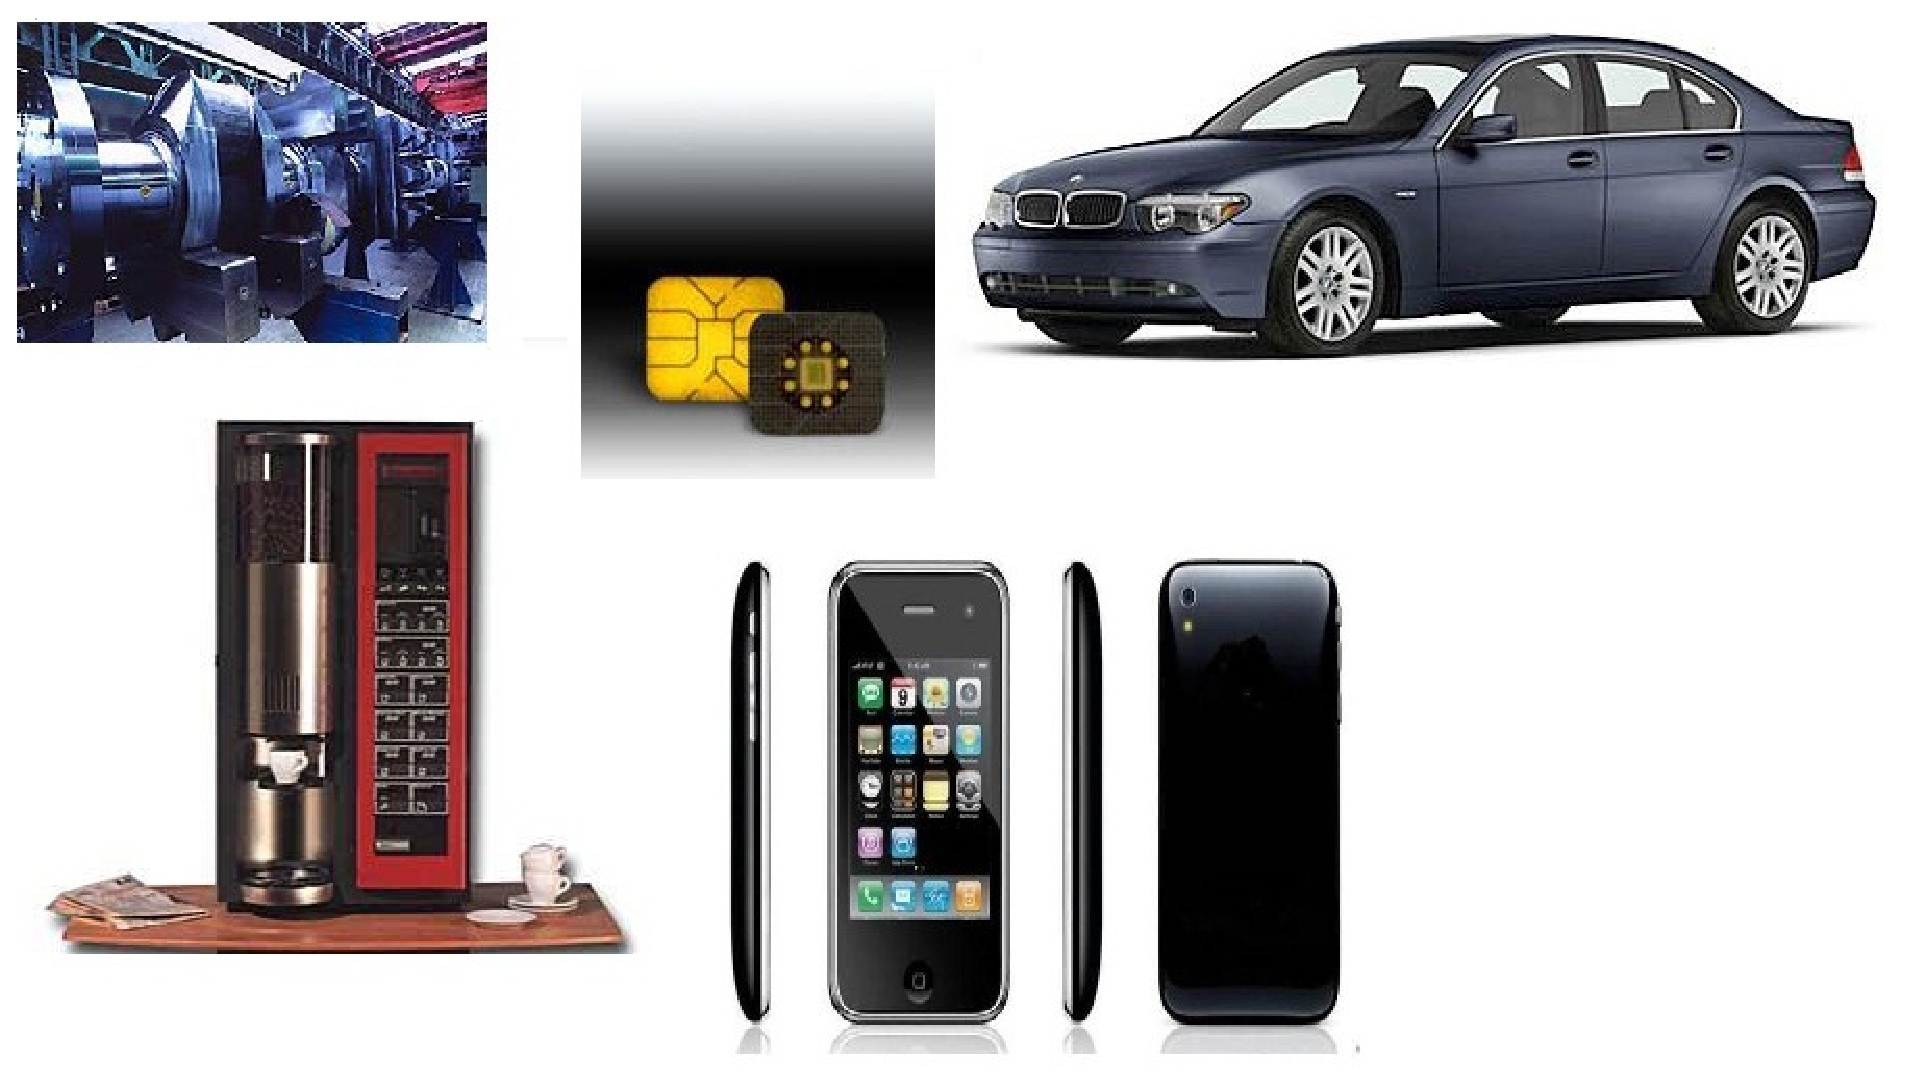
\includegraphics[scale=0.5, width =\columnwidth]{Figures/usos}
\end{center}
  \caption{Example of systems where formal methods are (can be) used .}
  \label{fig:uso}
\end{figure}

In the past, the use of formal techniques in practice seemed to be utopian and unrealizable. 
Among other causes, the notations used to require a high mathematical background in
mathematics and, therefore, they were too complicated for the uninitiated in the topic. 
The techniques did not allow the system to be scalable and the existing tools were
too difficult to use or understand or even there were no tools for a particular 
technique or formalism. In addition, case studies were not convincing enough and, 
therefore, developers could not appreciate the usefulness of formalization. 
However, in the early 90s, it started to glimpse a new way in this area. 
For the specification of software, the industry began to use the language Z \cite{Abrial80} 
in order to obtain rigorous specifications. For hardware verification, major 
companies such as Intel and AMD started to use formal techniques such as \emph{model checking} 
or \emph{theorem proving} to supplement tests on simulators. This led to the description of larger case studies,
which was benefitial for the advance of this area since other developers started to consider the possibility of 
introducing the use of formal techniques into their development processes.
In Figure \ref{fig:uso}, one can observe different systems in which these techniques are currently
used to ensure proper operation. For instance, big companies (e.g Boeing and Airbus)
use formal languages to specify the requirements of the equipment as well as they use 
formal methods to verify the most critical systems in the aircrafts. Moreover, automotive
companies verify the most critical systems ( e.g. brake or airbag systems) using \emph{model checking}. 

The main advantages of using formal methods are:

\begin{itemize}
\item The use of mathematics as a base gives this approach a certain rigour.
\item Identify ambiguity and inconsistencies.
\item Facilitates the construction of consistent and \emph{deadlock-free} systems.
\item Provides customer confidence in the system.
\item There are many tools that support the existing techniques.
\item Find bugs early should save money.
\end{itemize} 

The main disadvantages (or beliefs) that slow the progress of this area are:

\begin{itemize}
\item It is believed that the use of formal methods slows the development process.
\item Many developers think it is difficult to work with formal specifications.
\item It does not guarantee the correctness of the implemented code (only the model
it is based).
\item Increasing system complexity causes an exponential increase
the complexity of the verification.
\end {itemize}

As commented previously, companies can use formal methods along the entire
development lifecycle of a system, both hardware and software. 
Here, we will focus on software since this Thesis studies different standards for building software components. 
Next, we describe the different phases in which designers can apply any formal technique. 

One of the most important part in the development of a system is the requirements specification. 
A specification can be seen as a technical document where the features and services needed 
to build a product are stated. Nevertheless, it can also include information on 
subsequent steps such as verification, validation, testing, etc. Therefore, 
this should be the first part in which the participants should apply formal methods, taking the 
required time to correctly specify the system since a neat and correct specification will influence the 
rest of the proccess.
Anyway, make a proper specification does not guarantee the absence of errors because the 
presence of faults is an intrinsic characteristic of the systems. In this sense, 
the simple act of writing the document helps engineers to find errors in the early stages 
of the development process, helping the company to save  money and time. 
In Figure \ref{fig:coste}, one can observe what is the effect (in money) of finding a bug
in the different phases. As can be observed, the cost of fixing a bug increases as 
we advance in the lifecycle and, therefore, it is recommended to find these bugs as soon as possible. 
In this Thesis, we propose a formal language and its visual model to specify web service compositions 
with distributed resources, but this will be presented in Chapter \ref{chapter:c3}.

\begin{figure}
\begin{center}
  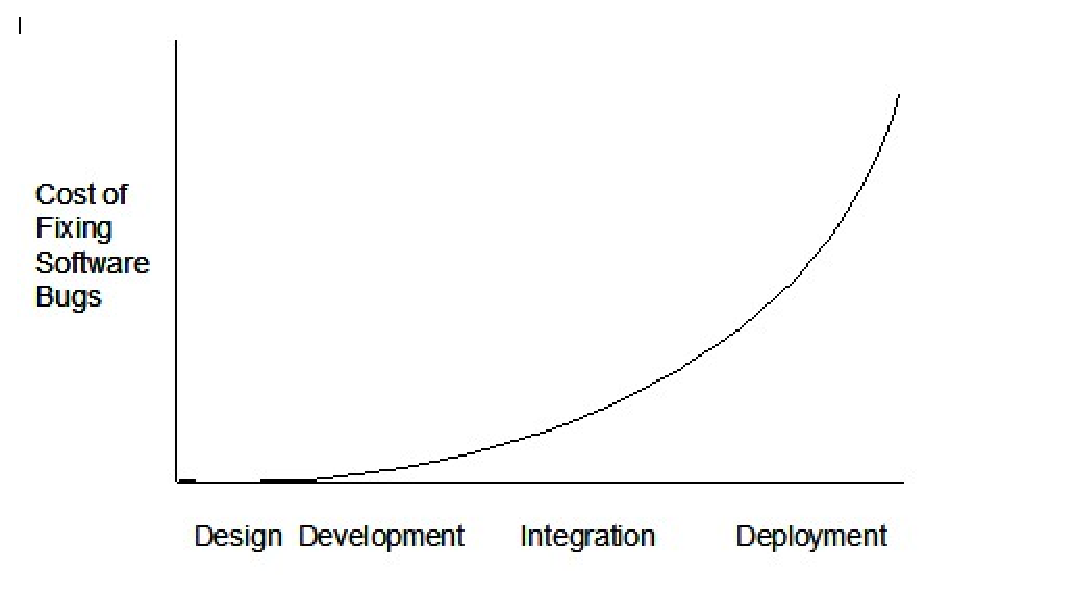
\includegraphics[scale=0.5, width =\columnwidth]{Figures/coste}
\end{center}
  \caption{Cost evolution of fixing a bug.}
  \label{fig:coste}
\end{figure}

In the classic life cycle, the verification and validation phases are performed after the implementation phase, 
but as we have seen in Figure \ref{fig:coste}, it is advisable to detect these errors as soon as possible. 
As expected, it is practically impossible to verify completely all the behaviour of a complex 
system so that the goal of researchers in this area is to check whether certain properties hold in the model. 
The properties of interest will be related to the classical problems of concurrency (\emph{deadlock, mutual exclusion,\ldots}) 
and some aspects directly related to the system itself such as check 
the adherence of it to certain time constraints. For example, in a banking system, 
it is mandatory to ensure that transactions meet the stipulated time for completion 
because if you exceed these restrictions some security issues could come out.

In this sense, one can follow two different ways to perform 
the verification of a system: \emph{Human-directed proof or Automated proof}.
The first one is used when you want to strengthen the knowledge of the system 
rather than completely ensure the correctness of it, and, therefore, it is a person who check the properties manually. 
This variant improves the knowledge of the system, but it is time-consuming and 
error-prone due to the entire process is conducted for a human being. 
In the second approach (\emph{automated proof}) there are also two variants: \emph{automated theorem proving and model checking}. 
The \emph{automated theorem proving } is conducted by a program that tries 
to produce a formal proof of a system from scratch, giving a description of it, 
a set of logical axioms and a set of inference rules. On the other hand, model checking \cite{Clarke99} 
is a technique for verifying finite state concurrent systems. It has a number of advantages 
over traditional approaches that are based on simulation, testing, and deductive reasoning. 
In particular, model checking is normally automatic and usually quite fast. Also, if the design contains an error, 
model checking will produce a counterexample that can be used to pinpoint the source of the error. 
Here, the specification can be expressed in propositional temporal logic propositional 
normally LTL \cite{Pnueli77} or CTL \cite{Henzinger94} or some of its variants, 
and the system is represented as a graph of transitions between states. 
The main challenge in model checking is dealing with the state space explosion problem. 
When dealing with web systems, this problem occurs in systems with many components that can interact with 
each other or systems with data structures that have many different values. 
In such cases the number of global states can be enormous. 
Researchers have made considerable progress on this problem over the last ten years. 
% Typically , the client only available to the engineer high-level representation of the system (usually in natural language ) and the specification of the same , also in natural language. So any \ emph { model checker } ( Spin \cite{Holz04} , UPPAAL \cite {Larsen97}, etc.) Exits with an affirmative answer if the proposed design meets the specification or provides a counterexample to locate where it has the error.

 
\section{Web Services modelling}

Although the Web was initially intended for the exclusive use of human beings, 
many experts believe that it needs to evolve (probably through modular design 
and construction services) to better support for the automation of many tasks. 
The concept of \emph{service} provides a higher level of abstraction to organize 
large-scale applications and build more open environments, helping to develop 
applications with improved productivity and quality with respect to other approaches. 
As services are only a mean for building distributed applications, 
it is required to evaluate the different existing approaches in this area. 
Figure \ref{arch} shows an example of service-based architecture, 
where there are three main parts: a consumer, a provider (the servers) and a set of records, 
where the services are stored. The role of the providers is to publish and/or advertise the 
services offered in the records, where consumers can find and invoke them. 
Current standards that support interactions between web services provide a 
solid foundation for service-oriented architecture. 
The web architecture is a framework that can be reinforced with more 
powerful representations and techniques inherited from other approaches.

\begin{figure}
\begin{center}
  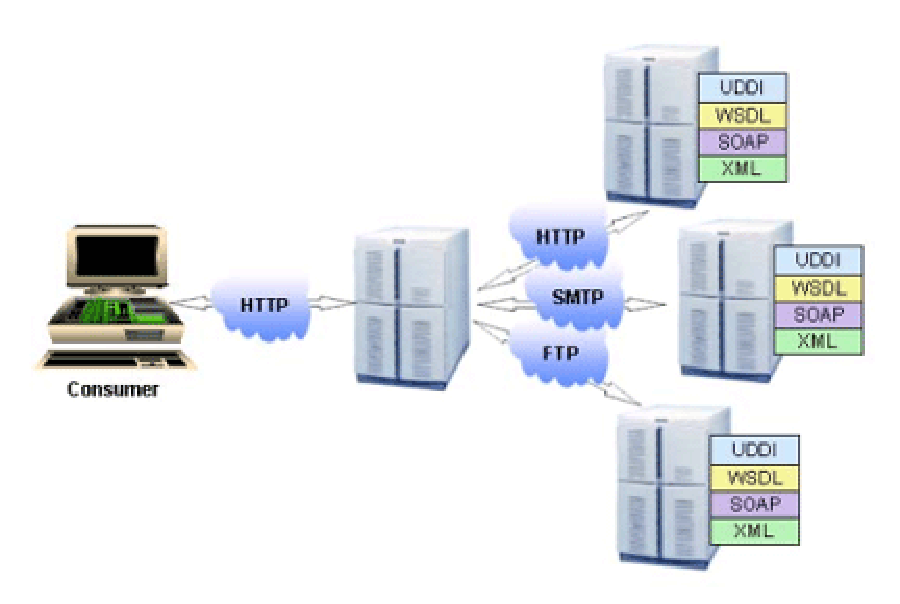
\includegraphics[width =\columnwidth]{Figures/clientserver.eps}
\end{center}
  \caption{Client-server web architecture}
  \label{arch}
\end{figure}

In this way, Service-Oriented Computing (SOC) paradigm promotes the use of services 
for the development of massively distributed applications, trying to achieve the creation of fast, 
low-cost, flexible and scalable applications \cite{Papazoglou2007}. 
Services are the main building block of this paradigm, being these services self-describing and platform-independent. 
Thanks to the use of standards for the description, publication, discovery and invocation, 
the services can be integrated without taking care of the low-level implementation 
details of each service. The aim of SOC is to make possible 
the creation of dynamic business processes and agile applications 
by providing an easy way to assemble application components into a loosely coupled network of services.

To reach the goals of SOC, a Service-Oriented Architecture (SOA) is defined. 
SOA is a software architecture based on the utilization of services, 
being these services provided to the user of the application or to other services in the network. 
This is possible by the use of service interfaces that can be published and discovered. 
SOA is based on a model of roles where every service can play multiple roles. 
For example, a service can offer certain functionality to a user and, at the same time, 
being the consumer of the functionality provided by some other services. 
Such model reduces the complexity of applications and increases their flexibility. 
Although at the beginning of SOA there were several architectures aspiring 
to become SOA standards \cite{Karp2000,Sun1999}, the most successful one was the architecture based on Web Services.

W3C defines a Web Service (WS) in the following way:

\begin{quotation}
	``A Web Service is a software system designed to support interoperable machine-to-machine interaction over a network. It has
an interface described in a machine-processable format (specifically WSDL). Other systems interact with the Web Service in a manner prescribed by its description using SOAP-messages, typically conveyed using HTTP with an XML serialization in conjunction with other Web-related standards.''
\end{quotation}

We can see in this definition that there are two basic standards 
related to Web Services: Web Service Description Language (WSDL) for the definition 
of the service functionality and its properties \cite{W3C2001}, 
and Simple Object Access Protocol (SOAP) for the exchange of 
XML messages between services \cite{W3C2007}. 
There is also an additional standard called Universal Description, Discovery and Integration (UDDI) 
used to create Web Service directories and to search for services 
in the network \cite{OASIS2004}, but this is a bit out of date. The use of these standard protocols is 
the key point to improve the integration between different parties in a web service architecture.

In Figure \ref{Figure1} a possible representation of the web service architecture stack is shown. 
One can see that the three standards described above are only a small part of the stack. 
One also need protocols to define security aspects (ensuring that exchanges of information 
are not modified or forgotten in a verifiable manner and that parties can be authenticated), 
to provide reliable messaging for the exchange of information between parties, 
to specify the collaboration between services when we compose them, 
to individually describe the behaviour of each service in a business process, etc. 
The problem is that whereas the standards for basic services (WSDL and SOAP) 
are widely adopted for their respective purposes, the situation is not very 
clear when we talk about composing services, 
having multiple protocols aspiring to become a standard in this layer.

\begin{figure}[h]
\begin{center}
\psfig{file=Figures/ws-stack.eps,scale=.55}
\end{center}
\caption{Web Service architecture stack.}
\label{Figure1}
\end{figure}

Two different approaches can be followed when we designing web service compositions. 
They are called \textit{orchestration} and \textit{choreography}. 
The former describes the individual business process followed by 
each one of the participants in the composition, 
while the latter describes the composition from a global viewpoint, 
defining the interactions (exchange of messages) happening between the parties, that is, 
how they collaborate in the composition. In Figure \ref{orch}, it is depicted graphically what it the role
of each of them if they are compared with the musicians in an orchestra. Despite these differences, the ideal solution would 
be fusing both approaches in a single language and environment \cite{Papazoglou2007}.

\begin{figure}[h]
\begin{center}
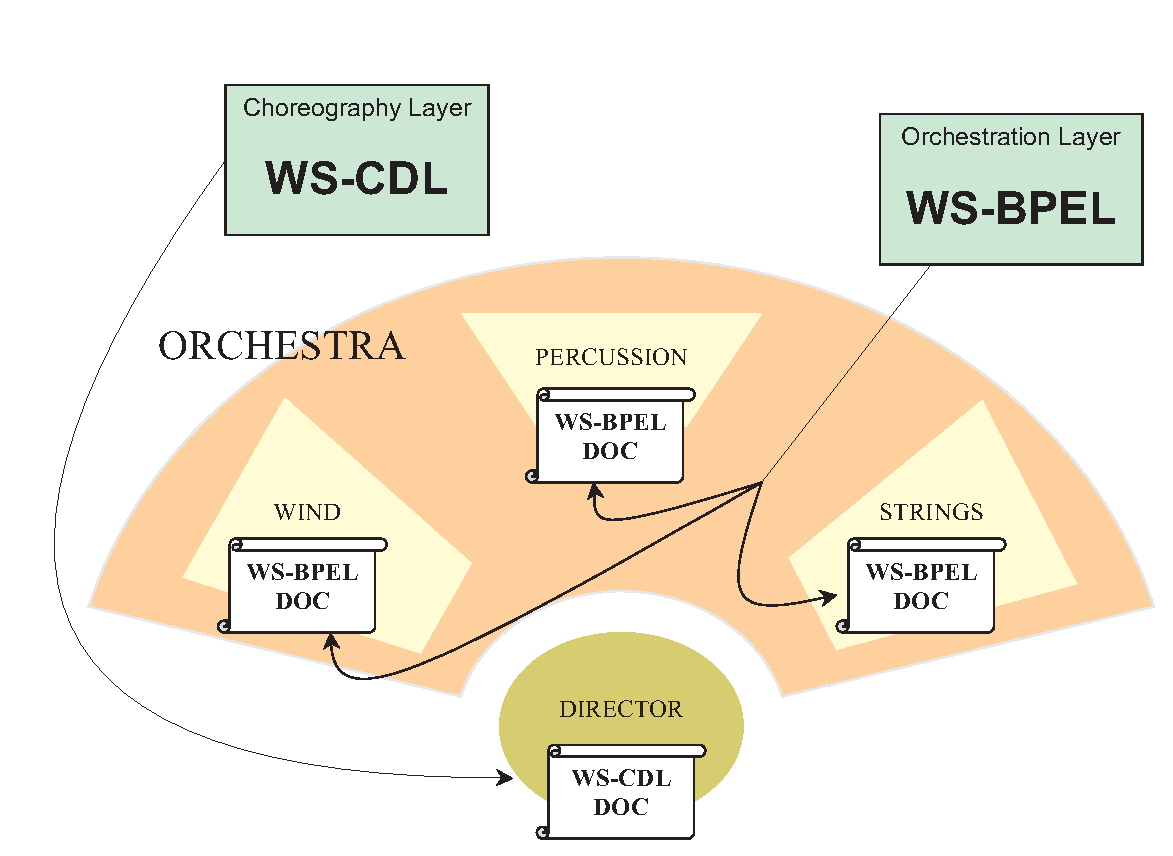
\psfig{file=Figures/orchestra.eps,scale=.5}
\end{center}
\caption{Choreography vs. Orchestration}
\label{orch}
\end{figure}

Anyway, the languages we can use in both cases should accomplish some common goals: 
(i) the capacity of modelling service interactions, including control flow and data constraints, 
(ii) the possibility of specifying exceptional behaviour, 
indicating which errors can happen in the execution of the composition 
and the way of handling these errors, and (iii) the ability to model web service compositions at a high level, 
without taking care of the implementation details of each one of the services.

Regarding the choreography approach, there are several languages that 
have been designed for that purpose. One of the most popular languages 
is Web Services Choreography Description Language (WS-CDL), 
which specifies the common and complementary observable behaviour of 
all participants in a composition \cite{W3C2005}. 
It is based on XML and describes the peer-to-peer collaborations 
between the composite web services from a global point of view, that is, 
the exchange of messages to achieve a common business goal. 
The aim of this language is allowing the composition of any kind of web services, 
regardless of the platform hosting the service or the implementation language. 
Figure \ref{Figure2} is an example of how WS-CDL can be useful 
for the integration of different kinds of web services.

\begin{figure}[h]
\begin{center}
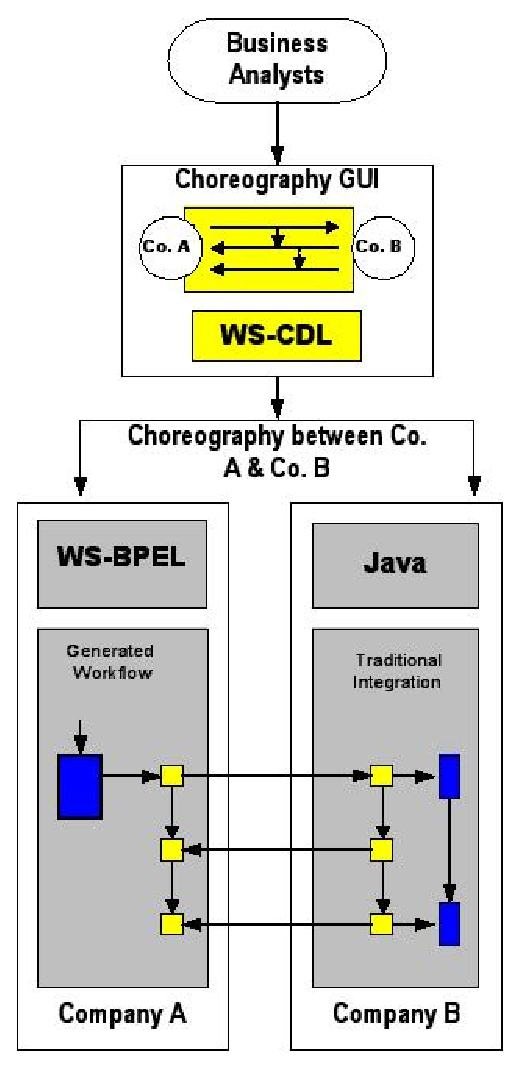
\psfig{file=Figures/WSCDL.eps,scale=.7}
\end{center}
\caption{Integration of Web Services using WS-CDL.}
\label{Figure2}
\end{figure}

A WS-CDL document defines a hierarchy of choreographies, where there is only one top-level choreography, marked explicitly as the \textit{root choreography}. The basic building block of a choreography is the \textit{interaction} element. It indicates information exchanges between participants, possibly including the synchronization of some information values. These interactions are performed when one participant sends a message to another participant in the choreography. When the message exchanges complete successfully, the interaction completes normally. 

We can distinguish two different kinds of \textit{complex activities} inside a choreography: the workunit element and the ordering structures. The \textit{workunit} element specifies a condition that must be fulfilled in order to perform some work and/or the repetition of some work. It completes successfully when the set of activities inside completes successfully. \textit{Ordering structures} are used to combine basic activities and other complex activities in a nested way, expressing the order in which actions are performed within the choreography. There are three ordering structures: The \textit{sequence} ordering structure expresses that the set of activities inside must be executed sequentially. The \textit{parallel} ordering structure indicates that the set of activities inside must be executed concurrently. It completes successfully when all the concurrent activities complete successfully. And the \textit{choice} ordering structure specifies that only one of multiple activities can be executed. If the choice have workunits inside, only the first one in lexical order with a ``true'' guard condition is selected. If there are other activities, there is no way to know which one is selected; it is considered as a non-observable decision.

Different types of exceptions are considered in WS-CDL. Exception workunits can be defined to handle all these exceptions. They may also be used as the mechanism to recover from the exceptions. At least one exception workunit must be defined. The guard of the workunit can be used to specify the particular type of exception we want to handle. Only one exception workunit can match each exception. If multiple exception workunits are defined, the order of evaluating them is based on the order in which the workunits have been defined. When the matching happens, the actions of the matched workunit are executed. If no matching happens and a default exception workunit exists, then the actions of this workunit are executed. Otherwise, the exception is raised in the parent choreography. WS-CDL also allows us to define finalization actions within a choreography that can confirm or cancel the effects of this choreography, so we can use this actions for compensation. 

\subsection {WS-BPEL}
In 2002, researchers and engineers of the main companies of the world (IBM, Microsoft, etc.)
realised that the new and rapidly emerging process-oriented approach required the definition of 
a neat and precise language for describing how a set of intecting web services can be included
in a business process. Traditional methods for integration and business process automation 
typically involve embedded logic inside of applications designed 
to meet a specific business need such as ERP, supply chain, or CRM. 
The development, testing, and deployment efforts required 
to change these applications make integration and process changes both costly and complex \cite{}.
To address these issues, proprietary products emerged 
to abstract integration and process automation into a new layer of software tools. 
These software products liberated integration and process tasks from 
the underlying business systems so they could be more effectively changed, managed, and optimized.
The idea and motivation behind almost each new technology and platform for
enterprise application development is to provide an environment where better
business applications can be developed with less effort and these business applications
should closely align to the business processes, which should not be too complex, and
which can be adapted to the changing nature of business processes without too much
effort. Within companies, business applications have to
interoperate and integrate. Integrating different
applications has always been a difficult task for various functional and technology
related reasons \cite{}.

The Business Process Execution Language for Web Services (BPEL4WS), for short BPEL, 
was first conceived in July, 2002 with the release of the BPEL4WS 
1.0 specification. This first draft was initially developed by just three companies, IBM, Microsoft, and BEA. 
This document proposed an orchestration language inspired 
by previous variations such as Web Services Flow Language (WSFL), developed by IBM and XLANG specification language developed
by Microsoft. WSFL was designed by IBM and is based on the concept of directed graphs.
XLANG was designed by Microsoft and is a block-structured language. BPEL combines
both approaches and provides a rich vocabulary for description of business processes. After this first attempt, other major companies such as SAP and Siebel Systems joined the former ones to write
the version 1.1 of the BPEL4WS specification that was released less than a year later, in May of 2003. 
Fortunately, this brand new version received much more attention and vendor support, 
leading to a number of commercially available BPEL4WS-compliant 
orchestration engines \cite{}. Before publishing this release, 
the BPEL4WS specification was submitted to an OASIS 
technical committee in order to be evaluated so that the specification could be developed into an official and open standard.
This technical committee was active from April 2003 to May 2007, 
and, during this time, a lot of contributions and improvements were received. 
In April 2007, WS-BPEL version 2.0 was approved as an OASIS standard. 
As a proof of maturity, more than 37 organizations collaborated to develop WS-BPEL, including representatives of Active Endpoints, Adobe Systems, BEA Systems, Booz Allen Hamilton, EDS, HP, Hitachi, IBM, IONA, Microsoft, NEC, Nortel, Oracle, Red Hat, Rogue Wave, SAP, Sun Microsystems, TIBCO, webMethods, and other members of OASIS \cite{}.
Finally, in January 2008, another OASIS technical committee started 
to define a WS-BPEL extension to emcompass the definition of 
human interactions (``human tasks'') as part of a WS-BPEL process. Figure \ref{bpelevolution} summarises this evolution-

\begin{figure}[h]
\begin{center}
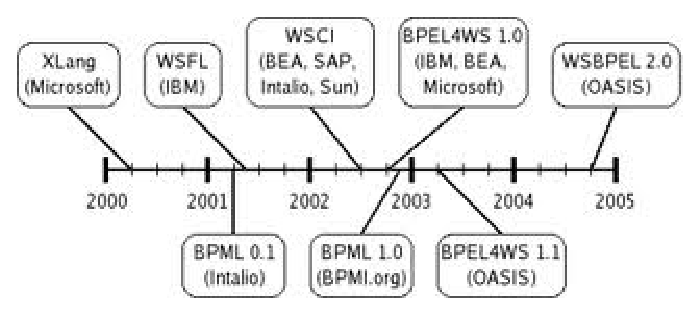
\psfig{file=Figures/bpelhistory.eps,scale=.7}
\end{center}
\caption{WS-BPEL evolution.}
\label{bpelevolution}
\end{figure}

Moreover, there were established ten original design goals associated with the definition of WS-BPEL \cite{wsbpelstandard}:
\begin{itemize}
\item Define business processes that interact with external entities 
through web service operations defined using WSDL, and that 
manifest themselves as web services defined using WSDL. 
\item Define business processes using an XML-based language. 
Do not define a graphical representation of processes or provide any particular design methodology for processes.
\item Define a set of web service orchestration concepts that are meant to be used by both the external (abstract) and internal (executable) views of a business process. Such a business process defines the behavior of a single autonomous entity, typically operating in interaction with other similar peer entities. 
%It is recognized that each usage pattern (i.e., abstract view and executable view) will require a few specialized extensions, but these extensions are to be kept to a minimum and tested against requirements such as import/export and conformance checking that link the two usage patterns.
\item Provide both hierarchical and graph-like control regimes, and allow their use to be blended as seamlessly as possible. This should reduce the fragmentation of the process modeling space.
\item Provide data manipulation functions for the simple manipulation of data needed to define process data and control flow.
\item Support an identification mechanism for process instances that allows the definition of instance identifiers at the application message level. Instance identifiers should be defined by partners and may change.
\item Support the implicit creation and termination of process instances as the basic lifecycle mechanism. Advanced lifecycle operations such as ``suspend'' and ``resume'' may be added in future releases for enhanced lifecycle management.
\item Define a long-running transaction model that is based on proven techniques like compensation actions and scoping to support failure recovery for parts of long-running business processes.
\item Use Web Services as the model for process decomposition and assembly.
\item  Build on Web services standards (approved and proposed) as much as possible in a composable and modular manner.
\end{itemize}

As a result, WS-BPEL along with web services technologies provide now a standardized integration interface 
and a standardized language for the integration of different services as well as for the automation of some tasks. 
Nevertheless, web scenarios are becoming more and more complex since they highly heterogeneous, that is, a lot of different
services from different companies interact jointly to perfom a particular task. In particular, it is known
that business processes change relatively often due to this heterogeneity. Therefore, designers 
do not need only a way to compose a set of services, rather they also
need a way to compose and modify them in the right order and in a relatively 
uncomplicated and straightforward way. Due to this, BPEL is sometimes compared 
to general purpose programming language, but it
is not as powerful as one of the well-known programming language \cite{}. However, 
it is simpler and better suited for business
process definition and, therefore, BPEL must be considered a supplement to
modern languages rather a replacement.

%The first version of BPEL has been developed in August 2002 by BEA, IBM, and
%Microsoft. Since then the majority of vendors have joined which has resulted in several
%modifications and improvements and adoption of version 1.1 in March 2003. In April
%2003, BPEL was submitted to OASIS (Organization for the Advancement of Structured
%Information Standards) for standardization purposes where the WSBPEL TC (Web
%Services Business Process Execution Language Technical Committee) has been formed
%since. This
%has led to even broader acceptance in industry.


%there are two possible ways to compose a set Choreography has not gained support from the
%industry which would be comparable to BPEL \cite{}.
%This is where the BPEL (Business Process Execution Language for Web Services, also
%WS-BPEL or BPEL4WS) becomes important. BPEL allows composition of web services
%and is thus the top-down approach to SOA ? the process oriented approach to SOA.
%Let us have a closer look at a typical BPEL process. First, the BPEL business process
%receives a request. To fulfill it, the process then invokes the involved web services and
%finally responds to the original caller. Because the BPEL process communicates with
%other web services, it relies heavily on the WSDL description of the web services
%invoked by the composite web service.

After briefly introduce its history and design goals, we discuss next its technical details. 
BPEL is therefore an orchestration
language in the sense that it is used to define the composition
of services from a local viewpoint, describing the individual
behaviour of each participant. Choreography is covered by other standards,
such as WS-CDL (commented previously). BPEL is designed to support the description of both behavioural service interfaces and executable
service-based processes \cite{OuyangVABDH07}. A behavioural interface (known as abstract process) is a specification of the
behaviour of a class of services, capturing constraints on the ordering of messages to be sent to and
received from a service. An executable process defines the execution
order of a set of activities (mostly communication activities), the partners involved in the process, the
messages exchanged between partners, and the events and exception handling specifying the behaviour
when specific events or faults occur. In Figure \ref{bpelexample}, we can observe an example of the typical business process
of a travel agency.

\begin{figure}[h]
\begin{center}
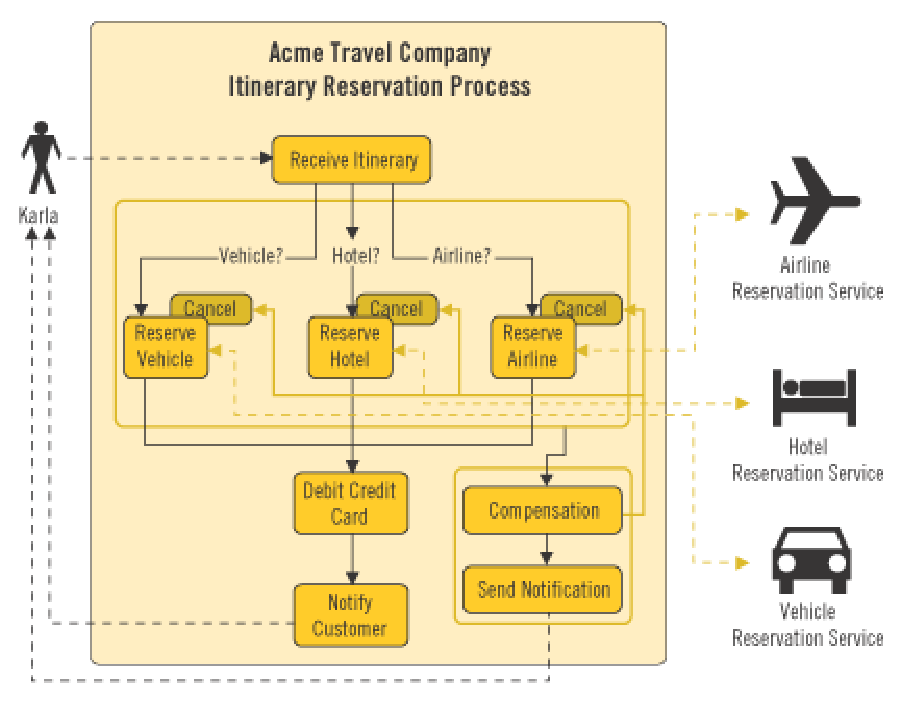
\psfig{file=Figures/bpelexample.eps,scale=.7}
\end{center}
\caption{Example of a business process workflow.}
\label{bpelexample}
\end{figure}

According to the standard of WS-BPEL, an  abstract process is a partially specified process that is not intended to be executed
and it must be explicitly declared as ``abstract''. As its name indicates, 
an abstract process may hide some of the required 
operational details expressed by an executable artifact.
All the constructs of executables processes are made available to abstract processes
and, consequently, they share the same expressive power \cite{}. 
Therefore, the main different between an abstract and a executable processes is 
that the second one contains the exact details of business processes and, consquently,
it is intended to be executed in an orchestration engine, whereas the first one serve a descriptive role,
defining the message exchange between the parties involved. Specifically, an abstract process is usually use to 
describe the observable behavior of some or all of the services offered by an
executable process and/or to define a process template that contains domain-specific best practices. 
Such a template can be seen as a design-time representation of the process logic, excluding execution details to be
completed when mapping to an executable process.
In most cases BPEL is used for
executable processes \cite{}.
Moreover, the definition of conceptual model in which one can define an abstract or an executable
process is a key feature of WS-BPEL since the processes execute and interact with their
partners in a consistent way regardless of the supporting platform or programming model used
by the implementation of the hosting environment, unlocking the potential of
web services because it allows the development of tools and other technologies that greatly
increase the level of automation and thereby lower the cost in establishing cross enterprise
automated business processes. In addition to this, abstract process ensures the level of privacy required by the 
companies since the implementation of the service is hidden to the other participants. 

In detail, WS-BPEL is an XML-based language which
supports the web services technology stack, including SOAP, WSDL, UDDI and so on. 
It defines a model and a grammar for describing the behavior of a business process
based on interactions between the process and its partners as well as the order of these interactions. 
The interaction with each partner is performed through web service interfaces, 
and the structure of the relationship at the interface level
is encapsulated in what is called a partnerLink. WS-BPEL also introduces 
mechanisms for dealing with business exceptions and faults. Moreover, WS-BPEL
introduces a mechanism to define how activities have to be compensated in cases 
where exceptions occur or a partner requests reversal.
A WS-BPEL process is a reusable definition that can be deployed in different ways and in
different scenarios, while maintaining a uniform application-level behavior across all of them.


\begin{figure}[h]
\begin{center}
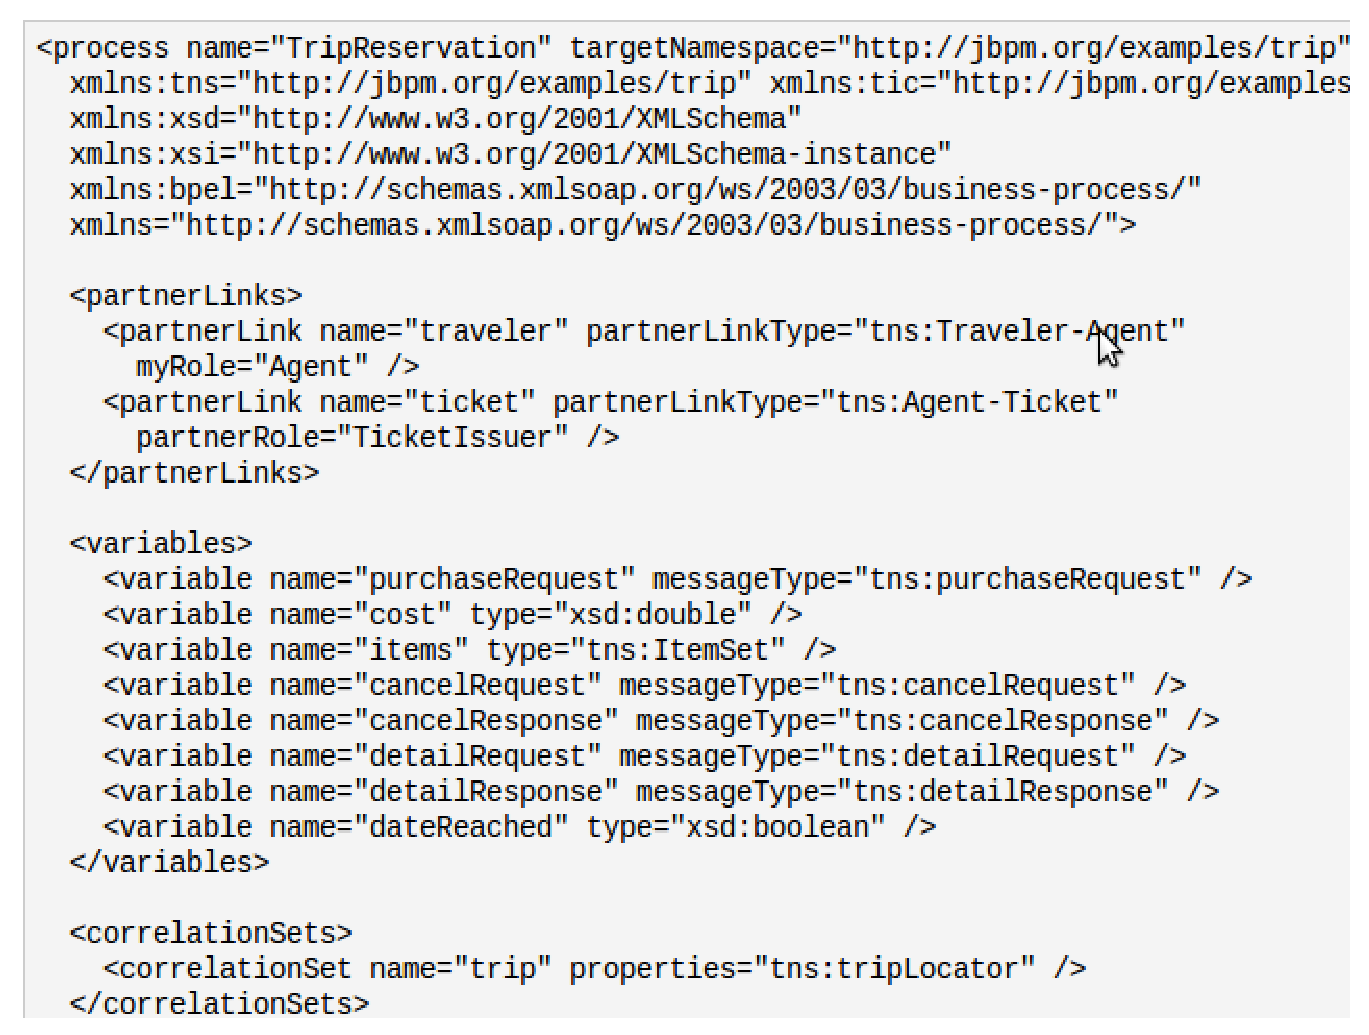
\psfig{file=Figures/bpelcode.eps,scale=.5}
\end{center}
\caption{WS-BPEL code.}
\label{bpelcode}
\end{figure}

In Figure \ref{bpelcode}, we can observe a piece of the BPEL code for a booking process. 
BPEL processes use {\em variables} to temporarily store 
data. Variables are therefore declared on a process or on a scope 
within that process. Also, 
it provides \emph{basic} or \emph{structured} to declare the process logic. 
\emph{Basic activities} are those which describe the elemental 
steps of the process behaviour \cite{}: 
\begin{itemize}
\item The activity \emph{assign} is used to assign data to the variables defined in the process. 
This activity can be used to copy data from one variable to another as well as to
populate new data in a variable using expressions. As usual, expressions are constructed using 
variables and constants. 
\item The activity \emph{empty} is devoted to be used as an activity that does nothing. For instance, one can
decide to capture an exception and do nothing to handle it. Another use of \emph{empty} is
to provide a synchronization point in a parallel activity.
\item The activity \emph{wait} specifies a particular delay or deadline. 
\item To invoke a web service of service provider, WS-BPEL offers the activity {\em invoke}. 
Normally, this activity is used to request an operation in a service. This operation is usually 
a basic activity in the provider. Operations can be of two types: request-response or one-way.
One-way consist of sending a message (some variables can be enclosed) so that no response is expected
as part of the operation, whereas a request-response invocation requires a message back. Evidently, this
response message can be used to notify the sender about a fault during the operation. A more detailed
explanation will be provided in Chapter \ref{chapter:c3}. 
\item A \emph{receive} activity is necesary to receive the message sent in the invoke activity.
messages, the portType (optional) and operation that it expects the partner to invoke. The
value of the partnerRole in the partnerLink is not used when processing a <receive> activity.
In addition, it specifies a variable, using the variable attribute, to
store the message the operation to be requested. In many cases, this activity is the first part of the process.
\item The \emph{reply} activity is used to respond to a request previously accepted through an
inbound message activity. For instance, it can be used in conjunction with the receive activity
to respond to the invocation of a service. Clearly, it is only meaningful
for request-response interactions, but a one-way ``response'' can be sent by invoking the
corresponding one-way operation on the sender. Finally, it may specify a
variable attribute that references the variable that contains the message data to be sent.
\item The activity \emph{throw} is used to signal an internal fault explicitly.
\item The activity \emph{exit} is used to immediately end the process instance.
\item WS-BPEL provides the user with the ability to declare new activities that are
not contemplated in the specification. This is done using the \emph{extension activities}. This
extension is not explicitly contemplated in the theory of this Thesis, although they are required
to implement the theory in an orchestration engine.
\item Finally, using the activity \emph{rethrow} in a fault handler, it is possible to rethrow a fault.
For instance, this activity is useful when the situation that causes the fault is not solved after
the completion of the fault handler and, therefore, it is needed to redo this handler to check if the
situation has been solved afterwards.
\end{itemize}  

On the other hand, \emph{Structured activities} encode the control-flow logic of the process.
The set of structured activities defined in the standard are the following:
\begin{itemize}
\item The activity \emph{sequence} includes a set of activities that are performed sequentially in the
order in which they appear in the structure. It ends
when the last activity in the sequence has finished.
\item The activity \emph{flow} provides concurrency and synchronization, creating 
a set of concurrent activities directly nested within the process and it enables
synchronization dependencies between activities that are nested to it. A more detailed explanation
of how this activity works is given in Chapter \ref{chapter:c3}.
\item The activity \emph{if} specifies conditional behavior. As usual, the activity consists of an ordered list of one or
more conditional branches defined by the ``if'' and optional ``elseif'' elements, followed by an
optional ``else'' element.
\item The activity \emph{while} provides conditional repetitive behaviour.
\item \emph{RepeatUntil} provides the repeated execution of a contained activity. The difference with
the activity while is that the inner activity is executed at least once.
\item The activity \emph{pick} waits for the occurrence of exactly one event from a set of events, and then
executes the activity associated with that event. After an event has been selected, the other events
are no longer accepted by that ``pick''. Moreover, a deadline for the occurrence of such events can be established
in such a way if this deadline experies the pick activity ends. This structure has some similarity the choice operator in
a process algebra althoudh with a predefined timeout. 
In WS-BPEL, it can be compared with a set of receive activities that run in parallel, where just only one can be executed,
and a common deadline for the execution of these receive activities is set (to this end, the wait activity can be used).
\item Lastly, the standard offeres an activity (forEach) to execute the contained activity a predefined number of times that
is expressed in the definition of the activity.
\end{itemize}

{\bf Comment}: Incluir foto orchesta y ventajas y desventajas choreographies and orchestations
Choreography on the other hand does not rely on a central coordinator. Rather, each
web service involved in the choreography knows exactly when to execute its operations
and whom to interact with. Choreography is a collaborative effort focused on exchange
of messages. All participants of the choreography need to be aware of the business
process, operations to execute, messages to exchange, and the timing of message
exchanges.
The most recent answer to the integration challenge is the Service Oriented
Architecture (SOA) and the web services technologies. The bottom-up view of the SOA
sees different business applications exposing their functionalities through web services.
Thus we can now access different functionalities of different legacy and new developed
applications in a standard way (through web services). Such access to functionalities is
important because typical companies have a large number of existing applications
which have to be integrated.

\section{Cloud Computing/Grid Computing}
Gracias a la r�pida evoluci�n que ha tenido la sociedad, servicios b�sicos para el desarrollo de la vida cotidiana son com�nmente suministrados a los ciudadanos, de tal manera, que cualquier persona puede tener acceso inmediato a ellos de forma f�cil. Hoy en d�a, estos servicios, conocidos en el mundo anglosaj�n como ``utility services'', engloban el suministro de agua, electricidad, gas y tel�fono, pero en los �ltimos tiempos est� cobrando fuerza una vieja idea que se intent� llevar a cabo sin �xito a finales de los a�os 60 y principios de los 70, el ``Utility Computing''. Este nuevo paradigma de computaci�n es normalmente confundido con Cloud o Grid Computing, pero hay ciertos matices que los diferencian. ``Utility Computing'' se puede entender como el modelo de negocio que subyace en una infraestructura Cloud o Grid, es decir, puede ser entendido como el medio de cobro de servicios computacionales similar al que se hace con la electricidad, por lo que el usuario pagar� s�lo por su consumo, mientras que los costes asociados a la producci�n y distribuci�n de potencia de c�mputo ser�n sufragados por las compa��as suministradoras. As�, las peque�as y medianas empresas podr�an competir en igualdad de condiciones con las grandes empresas, ya que no ser�a necesario hacer una gran inversi�n en datacenters para poder ofrecer un determinado servicio y se fomentar�a la creaci�n de empresas, ya que estos datacenters suponen una fuerte inversi�n inicial que muchos emprendedores no pueden acometer. Adem�s, el usuario final de las aplicaciones, servicios o infraestructuras tambi�n se beneficiar�a porque al reducir costes de producci�n se reduce el precio de los productos. Por seguir con el s�mil de la energ�a, podemos ver el cloud computing como una gran central generadora de energ�a que da suministro a millones de usuarios y que evita que dichos usuarios tengan que tener su propia central en casa para poder encender sus aparatos el�ctricos, mientras que el ``utility computing'' es la forma de tarificar el gasto de los usuarios o, de una forma m�s abstracta, podemos verlo como el contador que muestra el consumo energ�tico. Al igual que pasa con el software, los protocolos o cualquier paradigma relacionado con la inform�tica, Cloud Computing debe atravesar una serie de etapas para poder comprobar si toda esta publicidad que le est�n dando las empresas sirve de veras para ahorrar costes y favorecer la competitividad o solo es m�s una forma de aumentar ingresos o, en el caso de la investigaci�n, obtener nuevos fondos. En este sentido, algunos autores consideran que Cloud Computing no es mas que una nueva forma de nombrar lo que toda la vida se ha llamado Grid o Web Services y que realmente no supone ning�n avance en el campo de la inform�tica. Este art�culo tratar� de presentar m�s ampliamente la arquitectura y conceptos para comprender un sistema de computaci�n basado en la nube y mostrar� las diferencias entre dos enfoques cl�sicos de computaci�n (Grid y Web Services) y Cloud. Finalmente, se propondr� una serie de ideas que pueden llegar a convertirse en trabajos de investigaci�n en un futuro.         

\section{Introducci�n}

En 1943, el presidente de IBM, Thomas J. Watson, predijo:

\begin{center}
``I think there is a world market for about five computers''
\end{center}

Esta frase, tan comentada en el mundo de la inform�tica en los �ltimos tiempos, ha pasado de ser una predicci�n con poco fundamento a ser una realidad en la actualidad.\\

Cloud Computing, el viejo sue�o de ofrecer servicios de computaci�n como utilidad, tiene el potencial de transformar gran parte de la industr�a inform�tica, haciendo el software m�s atractivo al ofrecerlo como servicio y moldeando la forma en que se dise�a y compra el hardware. Con este nuevo enfoque, cualquier emprendedor con buenas ideas para ofrecer servicios a trav�s de Internet no necesitar� realizar grandes inversiones en equipamiento para llevar a cabo su proyecto ni necesitar� contratar inicialmente mucho personal que gestione y mantenga dicho equipamiento. Adem�s, no tiene que realizar complicados estudios previos para calcular el n�mero de usuarios potenciales y evitar, as�, unos de los principales quebraderos de cabeza de los jefes de proyecto: el sobre-aprovisionamiento o el infra-aprovisionamiento. Estos dos conceptos junto con la elasticidad de recursos pueden ser considerados como claves en computaci�n en la nube, ya que el objetivo de reducir costes es directamente proporcional a la correcta estimaci�n de recursos en ``tiempo real'' y esta correcta estimaci�n s�lo se puede proporcionar si el sistema cumple la propiedad de elasticidad, es decir, que en un intervalo de tiempo relativamente corto aumentas y disminuyes los recursos dedicados a una tarea con un coste econ�mico bajo. Este enfoque puede hacer que, a primera vista, no se perciba la posibilidad de utilizar m�todos formales con este tipo de sistemas, puesto que normalmente se utilizan t�cnicas formales en el dise�o de sistemas con tiempos de respuesta cr�ticos como sistemas de navegaci�n de un avi�n, transporte de materiales peligrosos, etc. De esta manera, se hace inviable el uso de la computaci�n en la nube cuando se exijan tiempos de respuesta muy bajos, ya que, por ejemplo, un sistema de navegaci�n de un avi�n no puede esperar varios minutos a que se le asignen nuevos recursos para tomar una decisi�n. Sin embargo, si que hay otro tipo de sistemas en los que los m�todos formales y el cloud computing pueden converger, los sistemas de alta disponibilidad.\\

As�, utilizando t�cnicas formales se pueden dise�ar este tipo de sistemas y verificar la ausencia de fallos en su construcci�n. Por ejemplo, una tienda de venta online podr�a pasar de tener cientos de usuarios simult�neamente a miles de ellos en periodos como las vacaciones de Navidad, de manera que necesitar�a mucha mayor potencia de computaci�n si quiere satisfacer a todos los clientes y no perder ingresos ni nuevos clientes por no poder atender esa demanda. Para satisfacer esta necesidad, har�a un estudio preliminar de cuantas visitas como m�ximo puede tener en ese per�odo y comprar�a los datacenters necesarios para no tener problemas de congesti�n, lo que supone una inversi�n grande en infraestructura por parte de la compa��a, sin embargo, una vez acaba la campa�a navide�a la demanda de usuarios vuelve a ser de unos cientos y la empresa se encuentra con que tiene una potencia de c�mputo que no va a necesitar y, por tanto, no est� amortizando econ�micamente la inversi�n realizada. En este sentido, si la compa��a en lugar de comprar los datacenters hubiese comprado capacidad de c�mputo a un proveedor entonces habr�a amortizado en mayor medida el dinero invertido y no tendr�a m�quinas en sus oficinas que ocupan bastante espacio y que tienen unos niveles de carga de trabajo muy bajos.  \\


Cloud Computing se refiere tanto a las aplicaciones que se ofrecen como servicios a trav�s de Internet como al hardware y software que est� presente en los datacenters que proveen dichos servicios. Estos servicios se han referido normalmente como Software as a Service (SaaS). El datacenter en s� es lo que se considera la nube (o cloud). Desde el punto de vista del hardware, hay tres aspectos novedosos en Cloud Computing: 

\begin{enumerate}
\item La ilusi�n de tener recursos ilimitados bajo demanda eliminando a los usuarios la necesidad de aprovisionarse antes de acometer una tarea.
\item La eliminaci�n de la inversi�n inicial en equipamiento permitiendo a las compa��as empezar con pocos recursos e ir aument�ndolos cuando las necesidades aumenten.
\item La posibilidad de pagar por el uso de recursos de computaci�n a corto plazo seg�n se necesiten (por ejemplo, procesadores por hora o capacidad de almacenamiento de datos por d�a) y poder liberarlos cuando no sean necesarios. 
\end{enumerate}

Cloud Computing podr�a tener el mismo impacto en la producci�n de software que el que tuvieron las fundiciones de metal en la industr�a del hardware. En principio, las compa��as fabricantes de hardware necesitaban tener sus propias instalaciones donde fabricar los componentes que compon�an sus productos, lo que les supon�a un gran esfuerzo econ�mico para construir y operar estas instalaciones y, por consiguiente, hac�a que el precio de los equipos se doblase en cada nueva generaci�n. Sin embargo, la aparici�n de compa��as que fabricasen componentes favoreci� que empresas m�s peque�as pudiesen entrar en el mercado del hardware, copado hasta aquel entonces por Intel o Samsung, que eran las �nicas que pod�an hacer frente a este gran esfuerzo econ�mico. De manera similar, la computaci�n en la nube podr�a jugar el papel que hicieron las fundiciones, favoreciendo la competencia y evitando monopolios de grandes empresas. \\

Debido a que muchas empresas usan servicios software como base para su modelo de negocio, se presentan, a continuaci�n, los actores que formar�n parte de este escenario. Los \emph{Services Providers}(SPs) hacen accesibles los servicios a los \emph{Service Users} por medio de interfaces que se comunican a trav�s de Internet. Dado que uno de los objetivos de la nube es externalizar la provisi�n de servicios, se necesita la aparici�n de otro actor que ofrezca esta infraestructura como ``servicio'' llamado \emph{Infrastructure Provider}, migrando los recursos desde los SPs al IPs y, as�, los SPs pueden ganar flexibilidad y reducir costes como se puede ver en la figura \ref{act}. 

\begin{figure}[bth]
  \center
    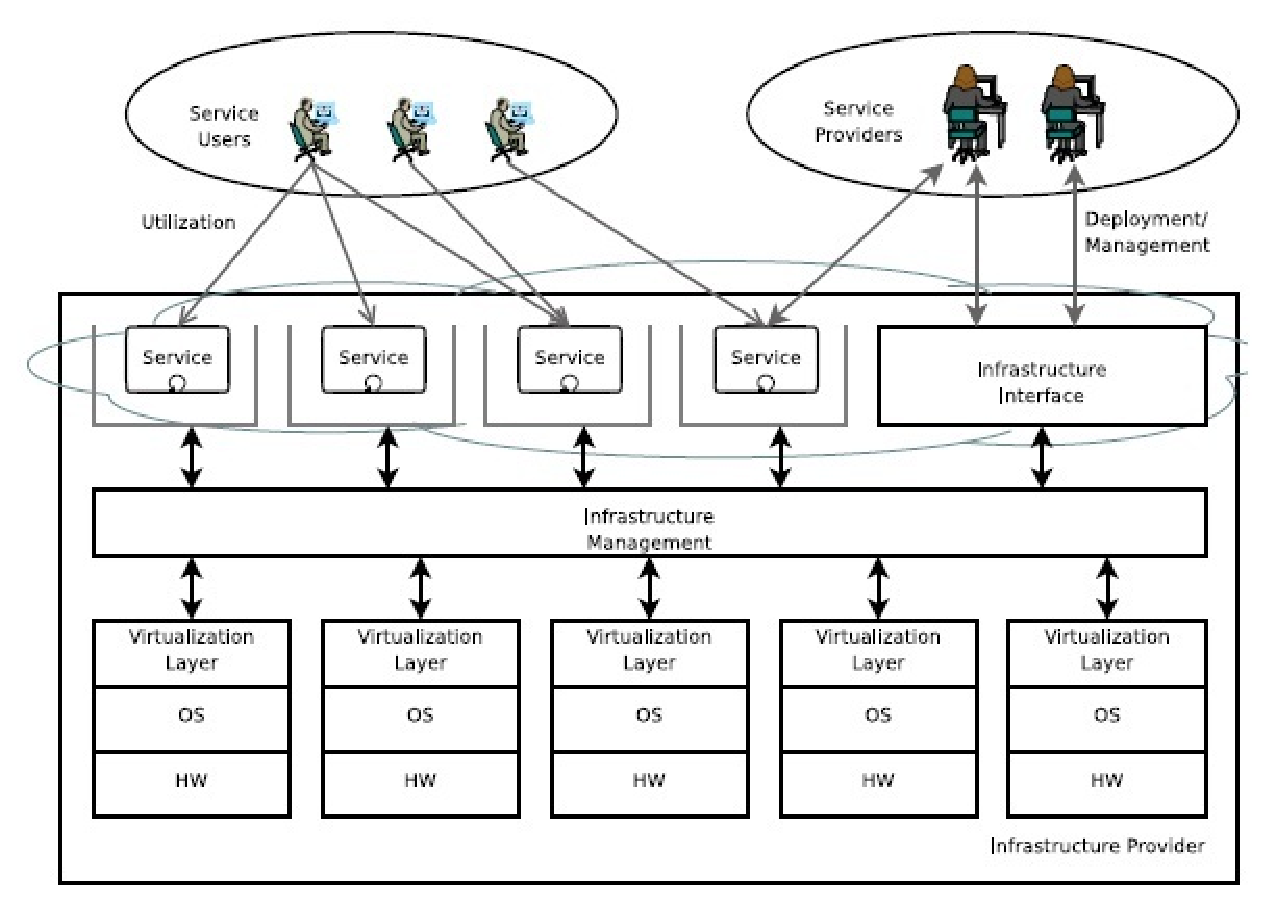
\includegraphics[scale=0.5]{Figures/actores}
  \caption{Actores en un sistema en la nube.}
  \label{act}
\end{figure}

\section{Comparaci�n entre servicios web y Grid computing/Cloud computing}

Como es sabido, nuestro grupo de investigaci�n ha centrado su investigaci�n en el desarrollo de una metodolog�a que permita construir y verificar sistemas con restricciones temporales mediante el uso de t�cnicas formales. En los �ltimos a�os, se ha aplicado esta metodolog�a en el �rea de los servicios web, m�s concretamente, en que estos servicios cumplan la tarea que se les encomienda y que se coordinen autom�ticamente para conseguir llevar a cabo un trabajo m�s general. El problema que est�n teniendo los servicios web es que como tuvieron un gran auge hace pocos a�os, muchos grupos de investigaci�n centraron sus estudios en este campo y, por tanto, hay muchos investigadores proponiendo nuevas aproximaciones y �sto ha llevado a que existen ciertas partes como BPEL o WS-CDL que est�n bastante estudiadas. De esta manera, esta surgiendo un sistema donde los m�todos formales pueden jugar un papel muy importante y donde nuestro grupo puede beneficiarse de su amplia experiencia tanto en formalizaci�n como en servicios web, el cloud computing. Este nuevo paradigma, como se ha expuesto anteriormente, est� viviendo su �poca de plenitud en este momento y grandes empresas como Google, IBM, Microsoft han decidido dar un paso al frente y apostar fuertemente por la computaci�n en la nube. Adem�s, muchos gobiernos est�n interesados en migrar sus servicios a la nube para abaratar costes y permitirles escalabilidad cuando les sea necesaria. Por ejemplo, hay que preguntarse si es necesario para la Agencia Tributaria tener grandes centros de datos cuando la demanda de servicios por parte de los ciudadanos s�lo crece en la �poca de la declaraci�n de la renta. Probablemente la respuesta sea afirmativa porque s� necesita almacenar todos esos datos y dar cierta confianza de que tus datos fiscales no van a caer en manos de gente con no muy buenas intenciones, pero toda la necesidad de c�lculo si que se puede externalizar para ahorrar costes en equipamiento o incluso podr�an crear una nube privada entre todos los organismos que colaboren con la agencia p�blica para compartir recursos e informaci�n. En este sentido, este tipo de sistemas donde la seguridad, privacidad y la disponibilidad son un requisito innegociable es donde podemos centrar parte de nuestras investigaciones e intentar mejorar alguno de los componentes de la arquitectura cloud expuesta en el apartado anterior. Por ejemplo, la mayor�a de grupos de investigaci�n desarrollan herramientas, pero la fase de pruebas o no existe o se le dedica poco tiempo. La semana pasada nos reunimos con uno de los grandes investigadores en el campo del Grid/Cloud Computing, Karim Djemame, y nos cont� que el principal problema que ten�a era ese que no sab�an concretamente porque funcionaba bien su herramienta y que estaba bastante interesado en la verificaci�n de su herramienta. \\


Por otro lado, a continuaci�n se enumeran algunas diferencias entre servicios web y grid/cloud computing para ver donde es posible aplicar nuestra experiencia en este sistema. En primer lugar, podemos considerar que los servicios web son en s� software que se ofrece como servicio (SaaS), aunque existan ciertas diferencias entre ambos enfoques, por ejemplo, la estandarizaci�n. Por tanto, este software podr�a estar compuesto de un conjunto de servicios, probablemente comunicados a trav�s de Internet, y que se coordinan para realizar una determinada tarea. Hasta el momento, nada nuevo, pero la principal diferencia reside en la virtualizaci�n, ya que los diferentes servicios que ofrece la nube se realizan en m�quinas virtuales en lugar de directamente sobre un servidor como puede ser el caso del servicio web, de manera que la concurrencia en el sistema es mayor. \\

Otra diferencia es la persistencia de los datos. Si queremos coordinar varios servicios web para que realicen sumas la �nica posibilidad de que �stos puedan almacenar el resultado es guard�ndolo en la base de datos, sin embargo, existe una aproximaci�n llamada WSRF (Web Services Resources Framework) que ha sido estandarizada y que resuelve este problema. En este framework cada servicio web lleva asociado un recurso o varios del sistema de manera que puedes interactuar con el servicio y decidir a que recurso acceder. La principal ventaja que tiene es que todos los servicios se definen con WSDL (Web Services Description Language) y que la comunicaci�n, direccionamiento, etc. est� estandarizado, de manera que la colaboraci�n entre sistemas de este tipo es sencilla. Otra ventaja es que el usuario tiene la posibilidad de decidir con que recursos interact�a. As�, podr�amos a�adir una capa inferior en nuestra metodolog�a que permitiese la definici�n de servicios web con recursos y una vez verificado que el sistema es correcto, desplegar estos servicios web en las m�quinas f�sicas. Este enfoque encajar�a perfectamente con nuestra investigaci�n, ya que utiliza servicios web con recursos y estos recursos tienen restricciones temporales para evitar que un usuario abarque todo el sistema. \\   

Tambi�n, podemos observar que cloud computing podr�a verse como una capa que se colocar�a debajo de los servicios web, ya que se puede utilizar �stos para acceder a los recursos, pero hay que resaltar que la nube no es solo ofrecer software como servicio, sino que tambi�n hay infraestructura y plataforma como servicio, cosa que los servicios web no pueden abarcar. Es decir, una parte del cloud computing (SaaS) puede compararse directamente con los servicios web, pero las otras dos partes no tienen nada que ver, por lo que ser�a como comparar el protocolo TCP/IP con la arquitectura de un PC, aunque es necesario que ambas aproximaciones (servicios web y cloud computing) converjan para el crecimiento de ambos paradigmas, igual que grid computing y servicios web convergieron en WSRF. \\

Por �ltimo, a modo de curiosidad la principal diferencia entre un sistema grid y uno cloud reside en la virtualizaci�n, ya que en grid el usuario no comparte en tiempo real los recursos que tiene asignados, mientras que en cloud es indispensable la virtualizaci�n de recursos para conseguir dar servicio a m�s clientes y conseguir ese ahorro que prometen los proveedores.

\section{Web Services Resource Framework(WSRF)}

La arquitectura que presentan los servicios web ha sido ampliamente aceptada como medio para estructurar las interacciones existentes entre los servicios que forman parte de un sistema distribuido y que colaborar para conseguir un objetivo com�n. En la actualidad, los desarrolladores requieren a los entornos una mayor estandarizaci�n para facilitar interoperatividad adicional entre dichos servicios, pero hasta mediados de 2004 ning�n grupo de investigaci�n o grupo de expertos se hab�a planteado seriamente la idea de proponer un est�ndar para modelar la comunicaci�n entre servicios web que poseen recursos persistentes asociados. As�, en Enero de ese a�o, varios miembros de la organizaci�n \emph{Globus Alliance} y de la multinacional inform�tica IBM definieron, con la ayuda de expertos de empresas como HP, SAP, Akamai, etc., la especificaci�n de los documentos que deber�an producirse en este modelo y la base de una arquitectura inicial. Estos documentos fueron enviados a la organizaci�n encargada de su estandarizaci�n, OASIS, en Marzo de 2004. En un principio, se formaron dos comit�s que se encargar�an del estudio y desarrollo de ciertas partes de este nuevo est�ndar. Por un lado, estaba el \emph{WSRF Technical Committee} que gestionaba cuatro especificaciones: \emph{WS-ResourceProperties, WS-ResourceLifetime, WS-ServiceGroup, y WS-BaseFaults}. Por otro lado, el \emph{WSN Technical Committee} se encargaba de las especificaciones: \emph{WS-BaseNotification, WS-Topics, y WS-BrokeredNotification}. \\

WS-Resource Framework est� inspirado en el trabajo realizado previamente por el \emph{Global Grid Forum's Open Grid Services Infrastructure (OGSI) Working Group} \cite{Foster03}. M�s concretamente, puede ser visto como una sencilla refactorizaci�n de los conceptos e interfaces desarrollados en la especificaci�n \emph{OGSI V1.0}, de manera que explota los recientes desarrollos en el �rea de los servicios web (por ejemplo, WS-Addressing). \\

El objetivo de este trabajo es introducir los conceptos fundamentales para la gesti�n y destrucci�n de servicios web persistentes, es decir, servicios web que llevan asociados recursos donde guardar los estados de los mismos, ya que hasta la aparici�n de esta aproximaci�n, los servicios web eran considerados ``\emph{stateless}'' y, por tanto, no pod�an almacenar temporalmente datos o resultados de sus operaciones de una manera sencilla para el usuario, ya que era necesario almacenarlos en una base de datos ajena al servicio. En este enfoque, es necesario codificar la relaci�n entre el servicio y el recurso en t�rminos de patrones utilizando una serie de tecnolog�as ampliamente estudiadas, como, por ejemplo, el WS-Addressing y, tambi�n, ser� necesario hacer sus propiedades accesibles desde el exterior a trav�s de un interfaz. En este sentido, llamaremos \emph{WS-Resource} a la asociaci�n entre un servicio web y un recurso persistente.  


\subsection{Introducci�n}

WS-Resource Framework \cite{Ban06} es una especificaci�n, desarrollada por OASIS y algunas de las empresas inform�ticas m�s pioneras, cuyo prop�sito es definir un marco gen�rico para el modelado y acceso a recursos asociados a servicios web, as� como las relaciones entre dichos recursos en un entorno Grid/Cloud. Esta aproximaci�n est� compuesta por un conjunto de especificaciones que definen la representaci�n del WS-Resource en los t�rminos que especifican los mensajes intercambiados y los documentos XML relacionados. Asimismo, incluye mecanismos que describen el medio para consultar el estado de un recurso y la descripci�n del servicio, que forman conjuntamente la definici�n de un WS-Resource. Adem�s, definen los pasos necesarios para hacer el estado de un servicio web accesible a trav�s de su interfaz (descrita en WSDL).\\

Normalmente, las interfaces de los servicios web proporcionan al usuario la posibilidad de acceder y manipular el estado del mismo, como, por ejemplo, valores de datos que evolucionan por la interacci�n entre varios servicios. En otras palabras, los intercambios de mensajes que se implementan en el comportamiento de los servicios tienen como objetivo permitir el acceso a estos recursos persistentes. Sin embargo, la noci�n de recursos persistentes que subyace en la implementaci�n de los servicios no es tan evidente en la definici�n de la interfaz \cite{Fost04}. Los mensajes que estos servicios env�an y reciben implican (o animan al programador a inferir) la existencia de un tipo de recurso asociado. Por tanto, es deseable que se definan est�ndares que permitan el descubrimiento, creaci�n, introspecci�n, interacci�n y destrucci�n de dichos recursos y que la forma elegida para llevar a cabo esta misi�n sea lo m�s interoperable posible. Estas observaciones han motivado la aparici�n de la propuesta comentada anteriormente, WS-Resource, para modelar estados en el contexto de los servicios web. Un WS-Resource se define como la composici�n de un servicio web y sus recursos persistentes asociados, esto es, \emph{(i)} expresado como una asociaci�n de un documento XML con un tipo definido con uno o varios \emph{portTypes} (un servicio podr� jugar un determinado rol si implementa todos los \emph{portTypes} que comprenden ese rol) y \emph{(ii)} direccionado y accedido de acuerdo al patr�n del recurso impl�cito, una derivaci�n de las \emph{Endpoint References} del WS-Addressing. Una \emph{Endpoint Reference} estar� compuesta por: Uniform Resource Identifier (URI), par�metros del mensaje que se envi� para solicitar el env�o de la \emph{Endpoint Reference} y datos relativos a la interfaz que se usa. En este intercambio, el identificador del recurso persistente es encapsulado en una \emph{Endpoint Reference} y usado para identificar al recurso en cualquier intercambio de mensajes entre los servicios que formen la coreograf�a. As�, WSRF permite declarar, acceder, monitorizar y destruir WS-Resources mediante mecanismos convencionales, lo que facilita la tarea de gesti�n, ya que no es necesario hacer m�s dif�cil la l�gica de decisi�n del servicio propietario del recurso para procesar los mensajes de gesti�n. Estos mecanismos convencionales componen cinco especificaciones t�cnicas que definen los medios por los cuales:

\begin{itemize}
\item Se destruye un WS-Resource, ya sea de manera s�ncrona con respecto a una petici�n expl�cita de destrucci�n o, a trav�s de un mecanismo basado en tiempos (scheduled). Adem�s, es posible declarar unas caracter�sticas espec�ficas  de los recursos (WS-ResourceProperties) que podr�an ser utilizadas para inspeccionar y monitorizar el tiempo de vida de dicho WS-Resource (WS-ResourceLifetime).
\item  Se definen los tipos de WS-Resource, que est�n compuestos por la interfaz de la descripci�n del servicio web (WSDL) y por un documento XML de propiedades del recurso. Por otro lado, el estado del WS-Resource puede ser consultado y modificado a trav�s del intercambio de mensajes (WS-ResourceProperties)
\item Un Endpoint Reference (WS-Addressing) puede ser renovado cuando su informaci�n de direccionamiento ha caducado o ha dejado de ser v�lida por alg�n error (WS-RenewableReferences).
\item Adem�s, se define la capacidad de implementar entornos heterog�neos como colecciones de servicios web, sean o no WS-Resources (WS-ServiceGroups).
\item La notificaci�n de errores puede ser m�s estandarizada al usar tipos XML Schema para definir los fallos base y definir reglas que muestren c�mo esos fallos son usados y extendidos (WS-BaseFaults).
\end{itemize}   

\subsection{WS-ResourceProperties}

Como se ha comentado anteriormente, WSRF utiliza una especificaci�n concreta para definir las propiedades del WS-Resource. Este recurso estar� compuesto por la definici�n de la interfaz en WSDL y un documento XML (Resource Properties Document) que especifica las propiedades del mismo, por ejemplo, el tama�o de disco, la capacidad del procesador, etc., de tal manera que si queremos acceder, modificar o actualizar este documento debemos utilizar una serie de mensajes preestablecidos en la especificaci�n. Las operaciones que se pueden hacer son las siguientes:

\subsubsection{GetResourceProperty}
Esta operaci�n como su propio nombre indica permite al servicio web que realiza la petici�n recuperar el valor de una {\bf �nica} propiedad del documento de propiedades. Para aclarar m�s los conceptos se define el siguiente ejemplo. \\


Dado el documento de propiedades:

\lstset{language=XML, numbersep=5pt,basicstyle=\small, frame=single}
\begin{lstlisting}
...
<GenericDiskDriveProperties 
xmlns: tns=``http://example.com/diskDrive'' >
  <tns:NumberOfBlocks>22</tns:NumberOfBlocks>
  <tns:BlockSize>1024</tns:BlockSize>
  <tns:Manufacturer>DrivesRUs</tns:Manufacturer>
</GenericDiskDriveProperties>
...
\end{lstlisting}

Una posible petici�n puede ser:

\lstset{language=XML, numbersep=5pt,basicstyle=\small, frame=single}
\begin{lstlisting}
...
<s12:Body>
  <wsrp:GetResourceProperty 
    xmlns:tns=``http://example.com/diskDrive''>
     tns:NumberOfBlocks
  </wsrp: GetResourceProperty>
</s12:Body>...
\end{lstlisting}

\subsubsection{GetMultipleResourceProperties}
Este m�todo es equivalente al anterior, pero para acceder a m�s de una propiedad del documento en el mismo mensaje, es decir, se utiliza para evitar congestionar la red. El mensaje enviado ser�a:


\lstset{language=XML, numbersep=5pt,basicstyle=\footnotesize ,frame=single}
\begin{lstlisting}
...
<wsrp:GetMultipleResourceProperties
 xmlns:tns=``http://example.com/diskdrive''>
 <wsrp:ResourceProperty>tns:NumberOfBlock</wsrp:ResourceProperty>
 <wsrp:ResourceProperty>tns:BlockSize</wsrp:ResourceProperty>
</wsrp:GetMultipleResourceProperties>
...
\end{lstlisting}

\subsubsection{SetResourceProperties}
Este m�todo se utiliza para realizar cambios en el documento de propiedades. Existen 3 tipos de cambios:

\begin{itemize}
\item Insert: Permite a�adir nuevas propiedades en el documento.
\item Update: Se utiliza para actualizar el valor de alguna propiedad.
\item Delete: Elimina propiedades del documento.
\end{itemize}

Un posible ejemplo de petici�n ser�a:

\lstset{language=XML, numbersep=5pt, basicstyle=\small,frame=single}
\begin{lstlisting}
...
<s12:Body>
 <wsrpw:SetResourceProperties
        xmlns:tns=``http://example.com/diskdrive''>
   <wsrp:Update>
    <tns:NumberOfBlocks>143</tns:NumberOfBlocks>
   </wsrp:Update>

   <wsrp:Delete resourceProperty=``tns:Manufacturer''/>

   <wsrp:Insert>
    <tns:someElement>42</tns:someElement>
   </wsrp:Insert>

 </wsrp:SetResourceProperties>
</s12:Body>
...
\end{lstlisting}


El documento de propiedades quedar�a con el siguiente formato:

\lstset{language=XML, numbersep=5pt, frame=single}
\begin{lstlisting}
...
<GenericDiskDriveProperties
  xmlns:tns=``http://example.com/diskDrive''>
  
  <tns:NumberOfBlocks>143</tns:NumberOfBlocks>
  <tns:BlockSize>1024</tns:BlockSize>
  <tns:someElement>42</tns:someElement>

</GenericDiskDriveProperties>
...
\end{lstlisting}

\subsubsection{QueryResourceProperties}
Como su propio nombre indica, este m�todo se utiliza para realizar consultas sobre propiedades del recurso. Por ejemplo si queremos saber si el n�mero de bloques es mayor que 20 y el tama�o de bloque es 1024 realizar�amos la siguiente consulta:

\lstset{language=XML, numbersep=5pt, frame=single}
\begin{lstlisting}
...
<s12:Body>
 <wsrp:QueryResourceProperties>
  <wsrp:QueryExpression
   Dialect=``http://www.w3.org/REC-xpath-19991116''>
    boolean(/*/NumberOfBlocks>20 and /*/BlockSize=1024)
  </wsrp:QueryExpression>
 </wsrp:QueryResourceProperties>
</s12:Body>
...
\end{lstlisting}

\newpage
La respuesta que env�a el otro servicio es:


\lstset{language=XML, numbersep=5pt, frame=single}
\begin{lstlisting}
...
<s12:Body>
 <wsrp:QueryResourcePropertiesResponse>
   true
 </wsrp:QueryResourcePropertiesResponse>
</s12:Body>
...
\end{lstlisting}


\subsection{WS-Base Faults}
El dise�ador de un servicio web normalmente utiliza interfaces definidas por otros, por lo que un m�todo que estandarizase el formato de los mensajes de notificaci�n de errores facilitar�a la labor de los desarrollares. �ste es el objetivo de WS-BaseFaults. Los mensajes de fallos en WSRF tienen el siguiente formato:


\lstset{language=XML, numbersep=5pt, frame=single}
\begin{lstlisting}
...
<BaseFault> 
  <Timestamp>xsd:dateTime</Timestamp> 
  <OriginatorReference> 
    wsa:EndpointReferenceType 
  </OriginatorReference> ? 
  <ErrorCode dialect=``anyURI''>xsd:string</ErrorCode>? 
  <Description>xsd:string</Description> * 
  <FaultCause>wsbf:BaseFault</FaultCause> * 
</BaseFault>
...
\end{lstlisting}
donde:

\begin{itemize}
\item Timestamp: Hora exacta cuando el fallo ha ocurrido.
\item OriginatorReference: Direcci�n en formato WS-Addressing del servicio que ha generado el fallo.
\item ErrorCode: C�digo de error para ser utilizado por sistemas de informaci�n de fallos, por ejemplo, POSIX errno.
\item Description: Explicaci�n de la causa del fallo (en lenguaje natural).
\item FaultCause: Causa t�cnica del fallo. 
\end{itemize}

\subsection{WS-ServiceGroup}
Esta especificaci�n permite crear grupos que comparten una serie de propiedades en com�n, es decir, agrupar diferentes servicios web que tienen comportamientos similares.

\subsection{WS-ResourceLifetime}

El tiempo de vida de un WS-Resource se define como el per�odo que transcurre entre su instanciaci�n y su destrucci�n. La misi�n de esta especificaci�n es estandarizar el proceso de destrucci�n de un recurso y definir mecanismos para monitorizar este ciclo de vida, pero lo que no se define es c�mo crear el WS-Resource. Generalmente, en los sistemas distribuidos, los clientes s�lo quieren tener un recurso por un determinado intervalo de tiempo, aunque en muchos escenarios es m�s apropiado para el cliente que se produzca la inmediata destrucci�n del recurso. Otro ejemplo claro de uso se presenta cuando el cliente quiere suscribirse a un servicio por un cierto tiempo y quiere que despu�s de este tiempo se destruya dicha uni�n. Como se coment� en la introducci�n, existen dos formas de destruir un recurso: inmediata, mediante un mensaje expl�cito o temporizada, mediante un mensaje que activa o gestiona un timer. 

\subsubsection{Destrucci�n inmediata}
Para la destrucci�n inmediata s�lo hace falta poner \emph{$<wsrl:Destroy/>$} dentro del cuerpo ($<Body>$) del mensaje SOAP que se env�a al servicio que gestiona el recurso y dicho servicio responder con \emph{$<wsrl:DestroyResponse/>$} dentro del cuerpo (\emph{$<Body>$}) del mensaje SOAP de respuesta.

\subsubsection{Destrucci�n temporizada}

En este caso, el WS-Resource tiene asociado un tiempo de terminaci�n que define el tiempo despu�s del cual se espera que el recurso haya sido destruido y, razonablemente, se espera que antes del mismo el recurso est� disponible. A continuaci�n se muestra un ejemplo de c�mo determinar el tiempo de terminaci�n de un recurso:

\lstset{language=XML, numbersep=5pt, frame=single}
\begin{lstlisting}
...
  <s12:Envelope
     <ex:ResourceDisambiguator>
      uuid:ba32-8680cace43f9
     </ex:ResourceDisambiguator>
     <s12:Body>
      <wsrl:SetTerminationTime>
       <wsrl:RequestedTerminationTime>
        2001-12-31T12:00:00
       </wsrl:RequestedTerminationTime>
     </wsrl:SetTerminationTime>
     </s12:Body>
  </s12:Envelope>
...
\end{lstlisting}



Como podemos observar el servicio que solicita la destrucci�n puede indicar la hora de destrucci�n y la hora actual (para evitar desajustes por la forma de representar la zona horaria). Una vez que CurrentTime alcanza el valor TerminationTime, el recurso se destruye sin ninguna intervenci�n m�s y se notifica al emisor del mensaje de destrucci�n que el recurso deja de estar disponible. Existe otro mensaje que se manda desde el receptor al emisor para comunicarle que ha recibido la petici�n de cambio.  \\

Sin embargo, puede darse la situaci�n de que haya m�s de un servicio utilizando el recurso que vaya a destruirse por lo que el propietario del recurso puede decidir o no (se deja a libre elecci�n del programador) implementar los mensajes WS-Notification para informar a los interesados que el recurso deja de estar disponible. Para llevar a cabo esta tarea debe crear este Topic: 

\newpage

\lstset{language=XML, numbersep=5pt, frame=single}
\begin{lstlisting}
...
<wstop:TopicSpace name=``ResourceLifetime''
   targetNamespace=
   http://docs.oasis-open.org/wsrf/2004/06/
   wsrf-WS-ResourceLifetime-1.2-draft-01.xsd
 
 <wstop:Topic name=``ResourceTermination''>
   <wstop:MessagePattern>
     <wsrp:QueryExpression
       dialect= http://www.w3.org/REC-xpath-19991116 >
        boolean(/*/TerminationNotification)
     </wsrp:QueryExpression>
 </wstop:MessagePattern>
...
\end{lstlisting}



Adem�s, el mensaje de notificaci�n asociado debe contener los siguientes campos: 


\lstset{language=XML, numbersep=5pt, frame=single}
\begin{lstlisting}
...
<wsrl:TerminationNotification>
 <wsrl:TerminationTime>xsd:dateTime</wsrl:TerminationTime>
 <wsrl:TerminationReason>xsd:any</wsrl:TerminationReason>?
</wsrl:TerminationNotification>
...
\end{lstlisting}
 
donde \emph{TerminationTime} informa de la fecha de destrucci�n y \emph{TerminationReason} contiene la explicaci�n de la destrucci�n.

\section{WS-Notification}

Esta especificaci�n permite a un \emph{NotificationProducer} enviar un mensaje de notificaci�n a un \emph{NotificationConsumer} de dos maneras diferentes:

\begin{enumerate}
\item El \emph{NotificationProducer} env�a un mensaje de notificaci�n al \emph{NotificationConsumer} sin seguir ning�n formalismo.
\item El \emph{NotificationProducer} utiliza el formalismo que se describe a continuaci�n para enviar las notificaciones. 
\end{enumerate} 

La opci�n a utilizar la elegir� el suscriptor cuando mande la petici�n de suscripci�n. En este sentido, la segunda opci�n permite al usuario recibir un amplio rango de mensajes de notificaci�n, ya que la informaci�n que se env�a en estos mensajes se obtiene de un �rbol de Topics (temas) y, por tanto, se permite enviar sub�rboles en un mismo mensaje para informar de diferentes Topics. En la Figura \ref{12} vemos un ejemplo:


\begin{figure}[h!]
  \center
    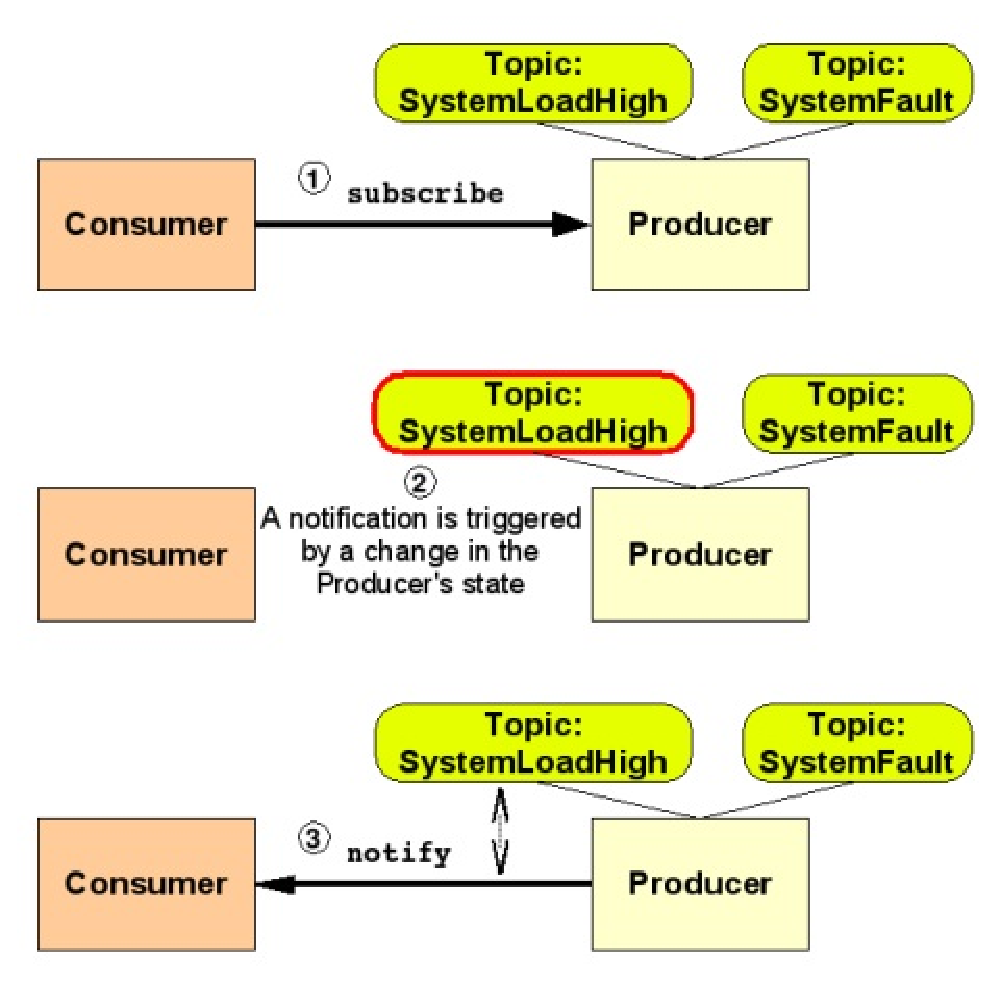
\includegraphics[scale=0.45]{Figures/12}
     \caption{Ejemplo de uso de WS-Notification sin broker.}
  \label{12}
\end{figure}
 
Este caso muestra un ejemplo de interacci�n entre un consumidor y un productor de notificaciones, en el caso de que el suscriptor y el consumidor sean la misma entidad. El sistema es simple ya que tenemos un consumidor y un productor que publica 2 topics: SystemLoadHigh y SystemFault. Los pasos necesarios son: 

\begin{enumerate}
\item En primer lugar, el consumidor se suscribe al topic SystemLoadHigh, por lo que internamente se crea un \emph{Subscription resource} con la informaci�n de la suscripci�n. El productor debe implementar un m�todo \emph{Subscribe} y el consumidor un m�todo \emph{Notify}.  
\item Despu�s, el productor debe enviar una notificaci�n cuando el sistema sobrepase una determinada carga de trabajo. Por ejemplo, nuestro sistema enviar� notificaciones cuando la carga de trabajo sea mayor de 50\%.
\item Por �ltimo, el productor env�a la notificaci�n invocando la operaci�n \emph{Notify} en el consumidor.
\end{enumerate}
   
Un ejemplo de mensaje \emph{Notify} es:
 
\lstset{language=XML, numbersep=5pt, frame=single}
\begin{lstlisting}
...
<wsnt:Notify>
    <wsntw:NotificationMessage>
     <wsnt:Topic Dialect= xsd:anyURI >
       {any}
     </wsnt:Topic>
     <wsnt:ProducerReference>?
      wsa:EndpointReference
     </wsnt:ProducerReference>
     <wsnt:Message>xsd:any</wsnt:Message>
    <wsnt:NotificationMessage>+
</wsnt:Notify>
...
\end{lstlisting}

Como podemos observar el mensaje \emph{Notify} contiene uno o varios mensajes de notificaci�n (\emph{NotificationMessages}). Los campos dentro de �stos son: 

\begin{itemize}
\item Topic: La informaci�n del topic que se env�a.
\item Dialect: El dialecto usado para expresar el topic anterior, es decir, el lenguaje utilizado para expresarlo.
\item ProducerReference: Direcci�n del productor.
\item Message: Una copia de la carga �til (payload) del mensaje actual.
\end{itemize}

A continuaci�n, se muestra el mensaje que manda el suscriptor para registrar su inter�s en uno o m�s topics:


\lstset{language=XML, numbersep=5pt, frame=single}
\begin{lstlisting}
...
<wsnt:Subscribe>
  <wsnt:ConsumerReference>
    wsa:endpointReference
  </wsnt: ConsumerReference>
  <wsnt:TopicExpression Dialect = xsd:anyURI >
    {any}
  </wsnt:TopicExpression>
  <wsnt:UseNotify>xsd:boolean</wsnt:UseNotify>?
  <wsnt:Precondition>wsrp:QueryExpression</Precondition>?
  <wsnt:Selector>wsrp:QueryExpression</wsnt:Selector>?
  <wsnt:SubscriptionPolicy>{any}</wsnt:SubscriptionPolicy>?
  <wsnt:InitialTerminationTime>
    xsd:dateTime
  </wsnt:InitialTerminationTime>?
</wsnt:Subscribe>

...
\end{lstlisting}


Los conceptos importantes en este mensaje son \emph{UseNotify} que se utiliza para decidir si el mensaje de notificaci�n sigue el formalismo WS-Notification o se manda sin formato, \emph{Precondition} que es la condici�n que genera mensajes de notificaci�n, es decir, si se cumple esta condici�n se generan mensajes, pero debe cumplirse tambi�n la condici�n \emph{selector} para enviarlos a los destinatarios que es la que se usa para decidir si se transmiten o no los mensajes generados. Adem�s, \emph{SubscriptionPolicy} se podr�a utilizar para controlar el ratio de env�o de mensajes(por ejemplo, no m�s de 3 por segundo) y \emph{InitialTerminationTime} contiene una sugerencia del tiempo de vida de la suscripci�n. WSRF tambi�n incluye mensajes para detener la suscripci�n, reanudarla o para que un servicio que acaba de unirse a una suscripci�n pueda obtener un historial de notificaciones sobre un determinado topic.



\subsection{WS-BrokeredNotification}

Un \emph{NotificationBroker} es un intermediario que, entre otras cosas, permite el env�o de mensajes entre uno o varios \emph{Publishers} y uno o varios \emph{NotificationConsumers}. La misi�n del \emph{Publisher} es observar ciertas situaciones y crear mensajes de notificaci�n para informar de esas situaciones, mientras que el broker es el encargado de distribuir estos mensajes. \\

En este caso, se pueden dar tres relaciones entre las partes: \emph{simple publishing}, \emph{composable publishing} y \emph{demand-based publishing}. En el primer caso, el \emph{Publisher} es el encargado de observar las situaciones y notificarlas al broker que ser� el encargado de transmitirlas a los interesados. En el segundo caso, el papel del \emph{Publisher} lo realizar� una entidad que implementa una serie de servicios especificados en WS-Notification (NotificationProducer). En este caso, el mensaje de notificaci�n puede llegar a otros consumidores que estuviesen suscritos al productor. En ambos casos, el broker puede pedir al \emph{Publisher} que se registre para poder publicar mensajes sobre un topic determinado. El �ltimo enfoque (\emph{demand-based publishing}) requiere que el \emph{Publisher} sea un \emph{NotificationProducer} y, as�, acepte mensajes de suscripci�n. El objetivo es reducir el n�mero de mensajes de notificaci�n haciendo que �stos solo se manden cuando se soliciten expresamente.





\subsection{Formal models of concurrency}\label{formalmodels}





\section{Summary}\label{sumArt}
\markright{~\ref{sumArt} Summary}

This chapter has described the state of the art of Service-Oriented Computing (SOC), the formalization of Web Service compositions, and the specification of electronic contracts (e-contracts).

The development of systems based on Web Services allows the creation of fast, low-cost, flexible and scalable applications, where the integration is possible thanks to the definition of multiple standard protocols (WSDL, SOAP, UDDI). However, the correct composition of Web Services is still an open problem, where different approaches can be followed, such as orchestration (BPEL) and choreography (WS-CDL, WSCI, OWL-S). The formal analysis of Web Service compositions by means of formal methods is therefore necessary to guarantee the correct composition.

Several formal techniques can be used for the analysis of Web Service compositions, being model checking one of the most popular. This is an automated technique consisting of the construction of a finite-state model of the system to check if
some properties are satisfied. Different specification formalisms can be used in model checking (process algebras, Petri nets, automata) and there are several tools supporting each one of these formalisms (CWB-NC, CPN Tools, UPPAAL).



%\chapter[Estado del Arte]{Estado del Arte}

En este cap�tulo se presenta el estado del arte en el campo de la especificaci�n, formalizaci�n y verificaci�n de servicios web, as� como los formalismos y herramientas necesarias para la comprensi�n y elaboraci�n de una futura tesis doctoral. El objetivo es mostrar al lector unas nociones b�sicas en formalizaci�n y servicios web que le facilitar�n la tarea de comprensi�n de la presente memoria.

\section{Introducci�n/Motivaci�n}

A lo largo de la historia de la computaci�n, los ingenieros han usado diferentes m�todos formales para mejorar la calidad del hardware y software. Estos sistemas con el incesante avance tecnol�gico en t�cnicas de integraci�n y metodolog�as de programaci�n crecer�n inevitablemente en escalabilidad y complejidad. Debido a esta complejidad, la probabilidad de error es mayor y, adem�s, alguno de estos errores pueden ocasionar incalculables p�rdidas econ�micas, de tiempo o, incluso, la p�rdida de vidas humanas. Por tanto, el principal objetivo de los ingenieros es facilitar a los desarrolladores la tarea de construir sistemas que tengan un �nfimo ratio de errores y que entren dentro de los m�rgenes comerciales de las empresas. Sin embargo, este tarea no es trivial porque necesitamos asegurar la correcci�n de las especificaciones y necesitamos proporcionar t�cnicas que ayuden a la detecci�n de errores y a la verificaci�n de los modelos desarrollados. Una de las v�as que los ingenieros han venido utilizando para conseguir este objetivo, como se ha comentado anteriormente, es la utilizaci�n de t�cnicas formales, que pueden definirse como el conjunto de procedimientos y herramientas basados en lenguajes matem�ticos que aseguran pr�cticamente la correcci�n de un sistema \cite{Clarke96} porque aumentan el nivel de conocimiento de un sistema, revelando inconsistencias y ambig�edades que no podr�an detectarse con otras t�cnicas, es decir, los m�todos formales ofrecen un mayor grado de refinamiento del modelo que otros m�todos. \\

\begin{figure}
\begin{center}
  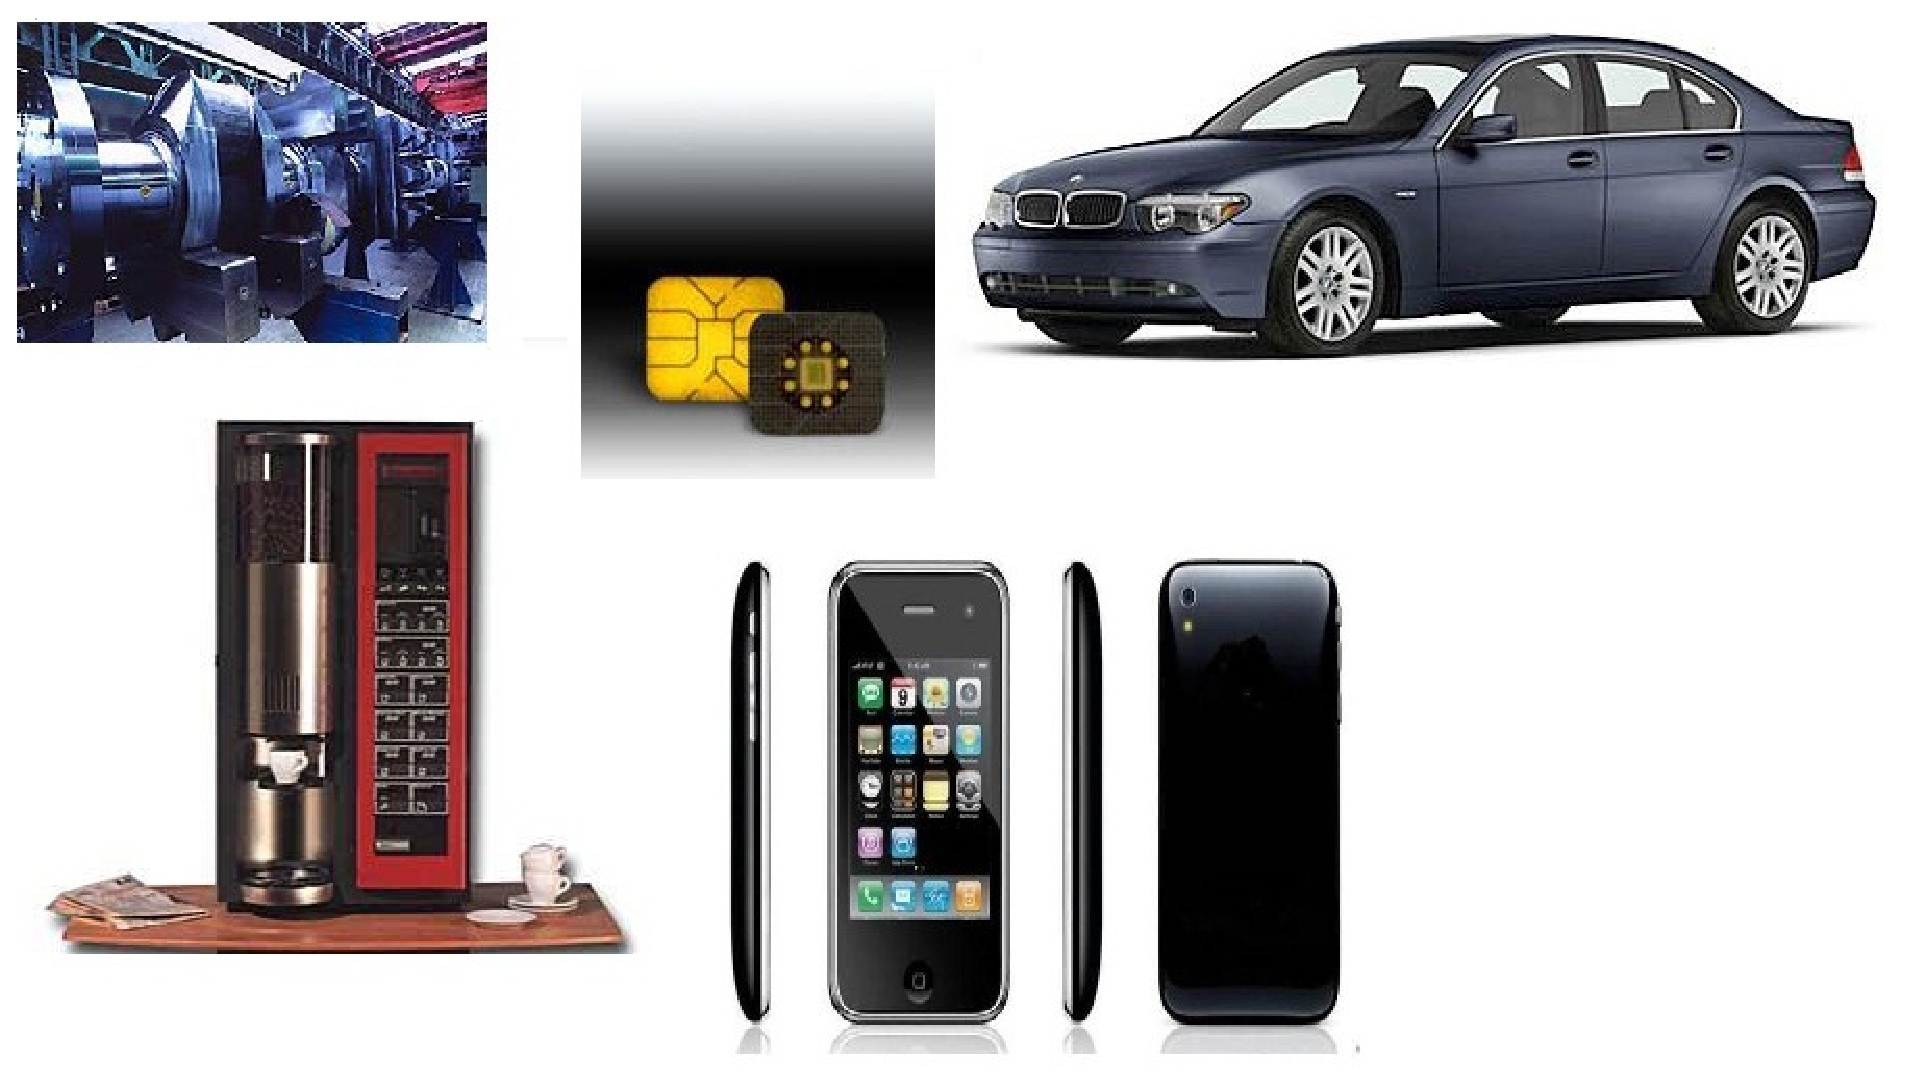
\includegraphics[scale=0.5, width =\columnwidth]{Figures/usos}
\end{center}
  \caption{Ejemplos de sistemas donde se usa la formalizaci�n.}
  \label{uso}
\end{figure}

En el pasado, el uso de t�cnicas formales en la pr�ctica parec�a no tener esperanzas porque las notaciones utilizadas eran demasiado complicadas para los no iniciados en la materia, las t�cnicas no permit�an que el sistema fuese escalable y las herramientas existentes eran demasiado dif�ciles de manejar o, incluso, no exist�an herramientas que modelasen una determinada t�cnica o formalismo. Adem�s, los casos de estudio que exist�an no convenc�an a los desarrolladores sobre la utilidad de la formalizaci�n. Sin embargo, a principios de los a�os 90, se empez� a vislumbrar un nuevo camino en este �rea. Para la especificaci�n de software, la industria empez� a utilizar el lenguaje Z \cite{Abrial80} para obtener especificaciones m�s rigurosas. Para la verificaci�n del hardware, las principales empresas del sector como Intel o AMD utilizan t�cnicas como el \emph{model checking} o \emph{theorem proving}  como complemento a las pruebas realizadas en los simuladores. En ambas �reas, tanto investigadores como desarrolladores est�n describiendo casos de estudio de mayor tama�o, lo que est� beneficiando a que otros desarrolladores est�n plante�ndose la posibilidad de implantar el uso de t�cnicas formales en sus procesos de desarrollo. En la Figura \ref{uso} podemos ver distintos sistemas donde se utilizan actualmente estas t�cnicas para asegurar el correcto funcionamiento de los mismos. Por ejemplo, las compa��as que fabrican aviones utilizan lenguajes formales para especificar los requisitos de los aparatos y las compa��as automovil�sticas verifican los sistemas m�s cr�ticos, en cuanto a seguridad se refiere, utilizando \emph{model checking}. \\

Las principales ventajas de utilizar t�cnicas formales son:

\begin{itemize}
\item El uso de las matem�ticas como base dota a este enfoque de cierto rigor.
\item Identifica la ambig�edad y las inconsistencias.
\item Facilita la construcci�n de sistemas consistentes y libres de \emph{deadlocks}.
\item Otorga confianza al cliente del sistema.
\item Existen multitud de herramientas que dan soporte a las distintas t�cnicas.
\item Encuentra fallos en etapas tempranas que ahorran mucho dinero.
\end{itemize} 

\newpage

Las principales desventajas (o creencias) que ralentizan el avance de este �rea son:

\begin{itemize}
\item Se cree que el uso de formalismos ralentiza el desarrollo.
\item Muchos desarrolladores piensan que es dif�cil trabajar con especificaciones formales.
\item No garantiza la correcci�n del c�digo implementado (s�lo la del modelo
en que se basa).
\item El aumento de la complejidad del sistema provoca un aumento exponencial
de la complejidad de la verificaci�n.
\end{itemize}

Una de las partes m�s importante en el desarrollo de un sistema es la especificaci�n de requisitos. En el �rea de la ingenier�a, una especificaci�n puede verse como un documento t�cnico donde se describen las caracter�sticas y servicios necesarios para construir un producto, aunque tambi�n puede incluir informaci�n sobre etapas posteriores como la verificaci�n, validaci�n, etc., por tanto, si queremos desarrollar sistemas correctos y de calidad debemos dedicar el tiempo necesario a la especificaci�n. De todos modos, realizar la especificaci�n no garantiza la ausencia de errores porque la presencia de fallos es una caracter�stica intr�nseca de los sistemas. En este sentido, el simple hecho de escribir el documento ayuda a los ingenieros a encontrar errores en fases tempranas del desarrollo ahorrando mucho dinero y tiempo al proyecto como puede verse en la Figura \ref{coste}. 

\begin{figure}
\begin{center}
  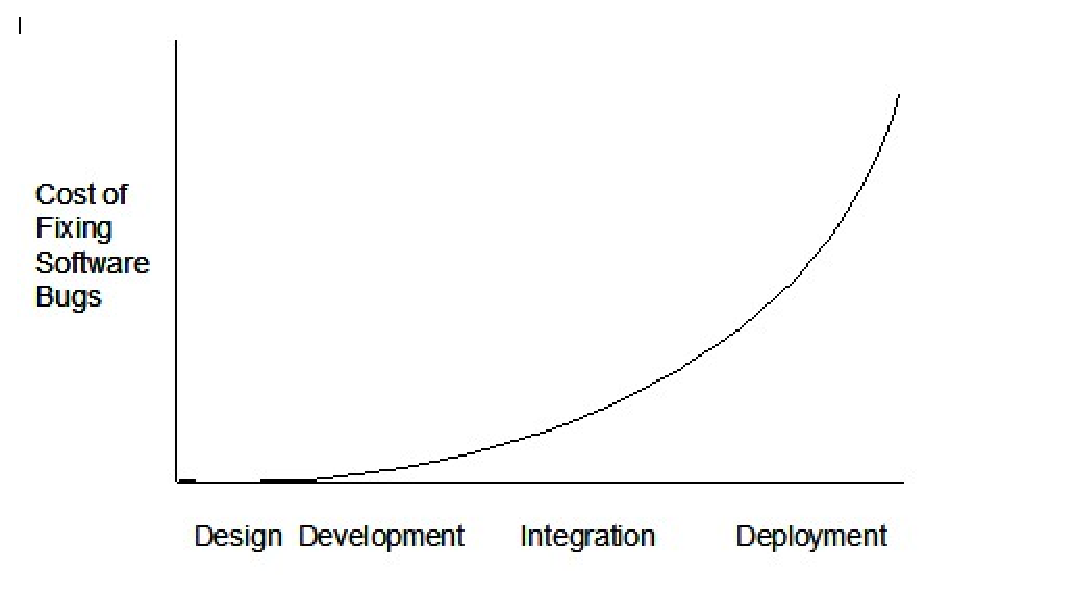
\includegraphics[scale=0.5, width =\columnwidth]{Figures/coste}
\end{center}
  \caption{Evoluci�n del coste de reparaci�n de un fallo.}
  \label{coste}
\end{figure}

\newpage

 
Otra fase del desarrollo donde se utilizan formalismos es en la etapa de \emph{Verificaci�n}. Se puede definir \emph{Verificaci�n} como la etapa donde se comprueba que el producto fabricado cumple con la especificaci�n de requisitos realizada previamente, es decir, en el caso de la inform�tica, que nuestro sistema cumple las propiedades que se describen en la especificaci�n. El objetivo de esta tarea puede resumirse en una de las frases m�s celebres de uno de los padres de los m�todos formales: \\
\begin{center}
\emph{``La verificaci�n de un programa s�lo muestra la presencia de errores, pero nunca garantiza la ausencia de los mismos''}
\end{center}
\vspace{-0.9cm}
\begin{flushright}
Edsger Wybe Dijkstra 
\end{flushright} 

En el ciclo de vida cl�sico, las fases de verificaci�n y validaci�n se realizan despu�s de la fase de implementaci�n, pero, como hemos visto en la Figura \ref{coste}, es necesario detectar estos errores en las fases tempranas del desarrollo. Como es de esperar, es pr�cticamente imposible verificar un sistema completo, por lo que el objetivo de los m�todos formales y de este trabajo de investigaci�n es comprobar si se cumplen ciertas propiedades en el modelo. Las propiedades de inter�s que es necesario verificar estar�n relacionadas con los problemas cl�sicos de concurrencia (\emph{deadlock, exclusi�n mutua, \ldots}), as� como algunos aspectos relacionados directamente con el sistema que se est� construyendo como puede ser comprobar si se cumplen ciertas restricciones temporales. Por ejemplo, en un sistema bancario es necesario verificar si las transacciones cumplen los tiempos estipulados para su realizaci�n, ya que si exceden estas restricciones podr�an ocasionarse problemas de seguridad en el sistema, lo que har�a perder mucho dinero al banco en cuesti�n. Otro ejemplo podr�a ser el sistema de reservas de una aerol�nea, ya que no podemos permitir que un usuario reserve un asiento durante un largo per�odo de tiempo porque podr�a no comprarlo finalmente y evitar que otro lo pudiera adquirir, con el consiguiente perjuicio para la compa��a. \\

Asimismo, se pueden seguir dos v�as para realizar la verificaci�n de un sistema: \emph{Human-directed proof o Automated proof}. El primer caso se utiliza cuando se quiere afianzar el conocimiento sobre el sistema en lugar de asegurar completamente la correcci�n del mismo, por lo que es una persona la que realiza de forma manual la verificaci�n. En la segunda aproximaci�n (\emph{automated proof}) tenemos dos variantes: \emph{automated theorem proving y model checking}. El \emph{automated theorem proving} consiste en que un programa trata de producir una prueba formal de un sistema desde el principio, dando una descripci�n del mismo, un conjunto de axiomas l�gicos y una serie de reglas de inferencia. Model checking \cite{Clarke99} es una t�cnica autom�tica para verificar sistemas reactivos de estados finitos. En esta aproximaci�n, la especificaci�n est� expresada en l�gica proposicional temporal, normalmente LTL \cite{Pnueli77} o CTL \cite{Henzinger94} o algunas de sus variantes, y el sistema se representa como un grafo de transiciones entre estados conocido como \emph{aut�mata}. En esta t�cnica debe utilizarse un eficiente m�todo de b�squeda para determinar si el aut�mata satisface la especificaci�n. El \emph{model checking} tiene numerosas ventajas sobre \emph{automated theorem proving}, pero la m�s importante es que el proceso tiene m�s partes que se pueden automatizar, por lo que la fase de prueba (\emph{testing}) dentro del ciclo de vida del sistema es m�s r�pida. Normalmente, el cliente s�lo pone a disposici�n del ingeniero una representaci�n a alto nivel del sistema (generalmente, en lenguaje natural) y la especificaci�n del mismo, tambi�n en lenguaje natural. As�, cualquier \emph{model checker} (Spin \cite{Holz04}, UPPAAL \cite{Larsen97}, etc.) termina el proceso con una respuesta afirmativa si el modelo propuesto satisface la especificaci�n o proporciona un contraejemplo para localizar d�nde se ha producido el error.
 

\section{Model Checking para Sistemas de Tiempo Real}

Los sistemas donde el tiempo juega un papel crucial para su funcionamiento y evoluci�n son conocidos como ``Sistemas de Tiempo Real (Real-Time Systems)''. Este tipo de sistemas son el n�cleo que controla la mayor�a de sistemas industriales, financieros y gubernamentales, donde el tiempo de respuesta determina el grado de correcci�n, la eficiencia, la satisfacci�n del usuario y otras variables de calidad, por lo que su correcto funcionamiento es vital para evitar errores que pueden ocasionar grandes p�rdidas. Sin embargo, dentro de estos sistemas existe otro tipo, donde las restricciones temporales juegan un papel realmente crucial, conocido como ``strong time restrictions''. En este entorno es necesario verificar completamente que el sistema tiene un ratio de error �nfimo porque un simple fallo podr�a ocasionar que el sistema dejara de funcionar. Otra informaci�n �til es la probabilidad de fallo cuando �ste no se puede eliminar. Esta medida sirve para dar confianza a los clientes, ya que un sistema con baja probabilidad de error aumenta el grado de satisfacci�n y confianza en el mismo. Esta informaci�n permite medir la necesidad de redise�ar el sistema o de mantenerlo en funcionamiento. En este caso, el fallo se debe a un factor externo que el sistema no puede manejar, como, por ejemplo, el tiempo, las leyes f�sicas o desastres naturales. Todos estos factores tienen en com�n que su aparici�n es incontrolable, pero es posible predecir su aparici�n con una razonable probabilidad. As�, existen sistemas donde la combinaci�n de ambas caracter�sticas, ``tiempo'' y ``probabilidad'', determinan las caracter�sticas principales del mismo, por lo que las t�cnicas de verificaci�n no s�lo tienen que tener en cuenta las restricciones temporales sino que deben considerar la probabilidad de que ocurran sucesos inesperados.      


\section[UPPAAL]{UPPAAL - Una herramienta para la verificaci�n autom�tica de Sistemas de Tiempo Real}

UPPAAL es una herramienta para la verificaci�n autom�tica de dos propiedades cruciales en los sistemas inform�ticos: \emph{safety} y \emph{liveness}, es decir, debemos asegurar que nuestro sistema es consistente (seguro) ante posible ataques o fallos y que permanecer� funcionando ante estos contratiempos \cite{Alur94}. El motor de UPPAAL transforma una clase de sistemas lineales h�bridos en redes de aut�matas temporizados e implementa t�cnicas basadas en la resoluci�n de restricciones. UPPAAL tambi�n ofrece valiosa informaci�n de diagn�stico en el caso de que la verificaci�n falle. Las siguientes secciones se centrar�n en aspectos formales de la herramienta.\\

La versi�n actual de la herramienta puede encontrarse en \textsf{http://www.uppaal.com}. A pesar de que fue desarrollada en 1995, actualmente cuenta con muchas caracter�sticas (probabilidades, costes, energ�a, etc.), gracias a la labor de investigaci�n realizada durante estos a�os. Debido a este alto grado de madurez y a la facilidad para conseguir informaci�n por las colaboraciones del grupo ReTiCS con la universidad de Aalborg, se ha seleccionado esta herramienta en lugar de otras. 




\section{Services Oriented Computing (SOC)}

Aunque la Web fue inicialmente concebida para el uso exclusivo del ser humano, muchos expertos consideran que tiene que evolucionar (probablemente a trav�s del dise�o y construcci�n de servicios modulares) para soportar mejor la automatizaci�n de muchas tareas. El concepto de \emph{servicio} proporciona un mayor nivel de abstracci�n para organizar las aplicaciones a gran escala y construir entornos m�s abiertos, ayudando a desarrollar aplicaciones con mejor productividad y calidad que las que podr�amos fabricar con otros enfoques. Puesto que los servicios son s�lo un medio para la construcci�n de aplicaciones distribuidas, no podemos hablar de ellos sin hablar de las aplicaciones basadas en servicios, en concreto, c�mo se construyen y c�mo los servicios deben funcionar conjuntamente dentro de ellas. La Figura \ref{arq} muestra un ejemplo de arquitectura basada en servicios, donde como puede observarse hay tres partes principales: un proveedor, un consumidor y un registro. 

\begin{figure}
\begin{center}
  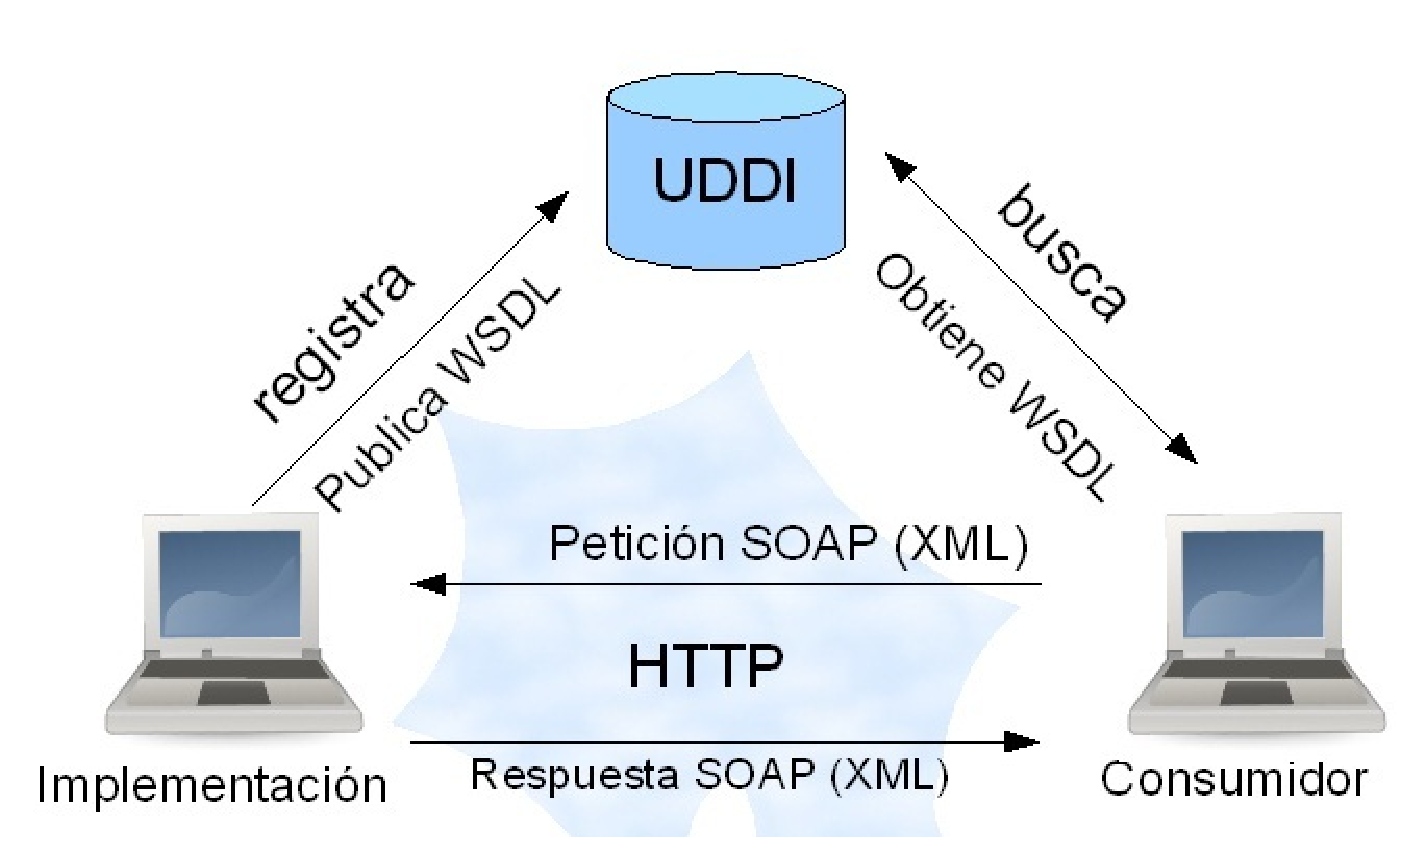
\includegraphics[width =\columnwidth]{Figures/arquitecturaWS}
\end{center}
  \caption{Arquitectura cliente-servidor para servicios web.}
  \label{arq}
\end{figure}

La funci�n de los proveedores es publicar o anunciar los servicios que ofrece en los registros, donde los consumidores pueden encontrarlos y, posteriormente, invocarlos. Los actuales est�ndares que sustentan las interacciones entre servicios web proporcionan una base s�lida para la arquitectura orientada a servicios, pero no soportan servicios esenciales para su funcionamiento completo. De hecho, aunque los servicios web proporcionan una fuente de ejemplos pr�cticos, son innecesariamente limitados. La arquitectura web es un marco que puede ser reforzado con representaciones m�s poderosas y t�cnicas tomadas de otros enfoques. Muchos profesionales utilizan estas representaciones, a pesar de que se omiten en la mayor�a de los libros. 

\section{Cloud Computing/Grid Computing}
Gracias a la r�pida evoluci�n que ha tenido la sociedad, servicios b�sicos para el desarrollo de la vida cotidiana son com�nmente suministrados a los ciudadanos, de tal manera, que cualquier persona puede tener acceso inmediato a ellos de forma f�cil. Hoy en d�a, estos servicios, conocidos en el mundo anglosaj�n como ``utility services'', engloban el suministro de agua, electricidad, gas y tel�fono, pero en los �ltimos tiempos est� cobrando fuerza una vieja idea que se intent� llevar a cabo sin �xito a finales de los a�os 60 y principios de los 70, el ``Utility Computing''. Este nuevo paradigma de computaci�n es normalmente confundido con Cloud o Grid Computing, pero hay ciertos matices que los diferencian. ``Utility Computing'' se puede entender como el modelo de negocio que subyace en una infraestructura Cloud o Grid, es decir, puede ser entendido como el medio de cobro de servicios computacionales similar al que se hace con la electricidad, por lo que el usuario pagar� s�lo por su consumo, mientras que los costes asociados a la producci�n y distribuci�n de potencia de c�mputo ser�n sufragados por las compa��as suministradoras. As�, las peque�as y medianas empresas podr�an competir en igualdad de condiciones con las grandes empresas, ya que no ser�a necesario hacer una gran inversi�n en datacenters para poder ofrecer un determinado servicio y se fomentar�a la creaci�n de empresas, ya que estos datacenters suponen una fuerte inversi�n inicial que muchos emprendedores no pueden acometer. Adem�s, el usuario final de las aplicaciones, servicios o infraestructuras tambi�n se beneficiar�a porque al reducir costes de producci�n se reduce el precio de los productos. Por seguir con el s�mil de la energ�a, podemos ver el cloud computing como una gran central generadora de energ�a que da suministro a millones de usuarios y que evita que dichos usuarios tengan que tener su propia central en casa para poder encender sus aparatos el�ctricos, mientras que el ``utility computing'' es la forma de tarificar el gasto de los usuarios o, de una forma m�s abstracta, podemos verlo como el contador que muestra el consumo energ�tico. Al igual que pasa con el software, los protocolos o cualquier paradigma relacionado con la inform�tica, Cloud Computing debe atravesar una serie de etapas para poder comprobar si toda esta publicidad que le est�n dando las empresas sirve de veras para ahorrar costes y favorecer la competitividad o solo es m�s una forma de aumentar ingresos o, en el caso de la investigaci�n, obtener nuevos fondos. En este sentido, algunos autores consideran que Cloud Computing no es mas que una nueva forma de nombrar lo que toda la vida se ha llamado Grid o Web Services y que realmente no supone ning�n avance en el campo de la inform�tica. Este art�culo tratar� de presentar m�s ampliamente la arquitectura y conceptos para comprender un sistema de computaci�n basado en la nube y mostrar� las diferencias entre dos enfoques cl�sicos de computaci�n (Grid y Web Services) y Cloud. Finalmente, se propondr� una serie de ideas que pueden llegar a convertirse en trabajos de investigaci�n en un futuro.         

\section{Introducci�n}

En 1943, el presidente de IBM, Thomas J. Watson, predijo:

\begin{center}
``I think there is a world market for about five computers''
\end{center}

Esta frase, tan comentada en el mundo de la inform�tica en los �ltimos tiempos, ha pasado de ser una predicci�n con poco fundamento a ser una realidad en la actualidad.\\

Cloud Computing, el viejo sue�o de ofrecer servicios de computaci�n como utilidad, tiene el potencial de transformar gran parte de la industr�a inform�tica, haciendo el software m�s atractivo al ofrecerlo como servicio y moldeando la forma en que se dise�a y compra el hardware. Con este nuevo enfoque, cualquier emprendedor con buenas ideas para ofrecer servicios a trav�s de Internet no necesitar� realizar grandes inversiones en equipamiento para llevar a cabo su proyecto ni necesitar� contratar inicialmente mucho personal que gestione y mantenga dicho equipamiento. Adem�s, no tiene que realizar complicados estudios previos para calcular el n�mero de usuarios potenciales y evitar, as�, unos de los principales quebraderos de cabeza de los jefes de proyecto: el sobre-aprovisionamiento o el infra-aprovisionamiento. Estos dos conceptos junto con la elasticidad de recursos pueden ser considerados como claves en computaci�n en la nube, ya que el objetivo de reducir costes es directamente proporcional a la correcta estimaci�n de recursos en ``tiempo real'' y esta correcta estimaci�n s�lo se puede proporcionar si el sistema cumple la propiedad de elasticidad, es decir, que en un intervalo de tiempo relativamente corto aumentas y disminuyes los recursos dedicados a una tarea con un coste econ�mico bajo. Este enfoque puede hacer que, a primera vista, no se perciba la posibilidad de utilizar m�todos formales con este tipo de sistemas, puesto que normalmente se utilizan t�cnicas formales en el dise�o de sistemas con tiempos de respuesta cr�ticos como sistemas de navegaci�n de un avi�n, transporte de materiales peligrosos, etc. De esta manera, se hace inviable el uso de la computaci�n en la nube cuando se exijan tiempos de respuesta muy bajos, ya que, por ejemplo, un sistema de navegaci�n de un avi�n no puede esperar varios minutos a que se le asignen nuevos recursos para tomar una decisi�n. Sin embargo, si que hay otro tipo de sistemas en los que los m�todos formales y el cloud computing pueden converger, los sistemas de alta disponibilidad.\\

As�, utilizando t�cnicas formales se pueden dise�ar este tipo de sistemas y verificar la ausencia de fallos en su construcci�n. Por ejemplo, una tienda de venta online podr�a pasar de tener cientos de usuarios simult�neamente a miles de ellos en periodos como las vacaciones de Navidad, de manera que necesitar�a mucha mayor potencia de computaci�n si quiere satisfacer a todos los clientes y no perder ingresos ni nuevos clientes por no poder atender esa demanda. Para satisfacer esta necesidad, har�a un estudio preliminar de cuantas visitas como m�ximo puede tener en ese per�odo y comprar�a los datacenters necesarios para no tener problemas de congesti�n, lo que supone una inversi�n grande en infraestructura por parte de la compa��a, sin embargo, una vez acaba la campa�a navide�a la demanda de usuarios vuelve a ser de unos cientos y la empresa se encuentra con que tiene una potencia de c�mputo que no va a necesitar y, por tanto, no est� amortizando econ�micamente la inversi�n realizada. En este sentido, si la compa��a en lugar de comprar los datacenters hubiese comprado capacidad de c�mputo a un proveedor entonces habr�a amortizado en mayor medida el dinero invertido y no tendr�a m�quinas en sus oficinas que ocupan bastante espacio y que tienen unos niveles de carga de trabajo muy bajos.  \\


Cloud Computing se refiere tanto a las aplicaciones que se ofrecen como servicios a trav�s de Internet como al hardware y software que est� presente en los datacenters que proveen dichos servicios. Estos servicios se han referido normalmente como Software as a Service (SaaS). El datacenter en s� es lo que se considera la nube (o cloud). Desde el punto de vista del hardware, hay tres aspectos novedosos en Cloud Computing: 

\begin{enumerate}
\item La ilusi�n de tener recursos ilimitados bajo demanda eliminando a los usuarios la necesidad de aprovisionarse antes de acometer una tarea.
\item La eliminaci�n de la inversi�n inicial en equipamiento permitiendo a las compa��as empezar con pocos recursos e ir aument�ndolos cuando las necesidades aumenten.
\item La posibilidad de pagar por el uso de recursos de computaci�n a corto plazo seg�n se necesiten (por ejemplo, procesadores por hora o capacidad de almacenamiento de datos por d�a) y poder liberarlos cuando no sean necesarios. 
\end{enumerate}

Cloud Computing podr�a tener el mismo impacto en la producci�n de software que el que tuvieron las fundiciones de metal en la industr�a del hardware. En principio, las compa��as fabricantes de hardware necesitaban tener sus propias instalaciones donde fabricar los componentes que compon�an sus productos, lo que les supon�a un gran esfuerzo econ�mico para construir y operar estas instalaciones y, por consiguiente, hac�a que el precio de los equipos se doblase en cada nueva generaci�n. Sin embargo, la aparici�n de compa��as que fabricasen componentes favoreci� que empresas m�s peque�as pudiesen entrar en el mercado del hardware, copado hasta aquel entonces por Intel o Samsung, que eran las �nicas que pod�an hacer frente a este gran esfuerzo econ�mico. De manera similar, la computaci�n en la nube podr�a jugar el papel que hicieron las fundiciones, favoreciendo la competencia y evitando monopolios de grandes empresas. \\

Debido a que muchas empresas usan servicios software como base para su modelo de negocio, se presentan, a continuaci�n, los actores que formar�n parte de este escenario. Los \emph{Services Providers}(SPs) hacen accesibles los servicios a los \emph{Service Users} por medio de interfaces que se comunican a trav�s de Internet. Dado que uno de los objetivos de la nube es externalizar la provisi�n de servicios, se necesita la aparici�n de otro actor que ofrezca esta infraestructura como ``servicio'' llamado \emph{Infrastructure Provider}, migrando los recursos desde los SPs al IPs y, as�, los SPs pueden ganar flexibilidad y reducir costes como se puede ver en la figura \ref{act}. 

\begin{figure}[bth]
  \center
    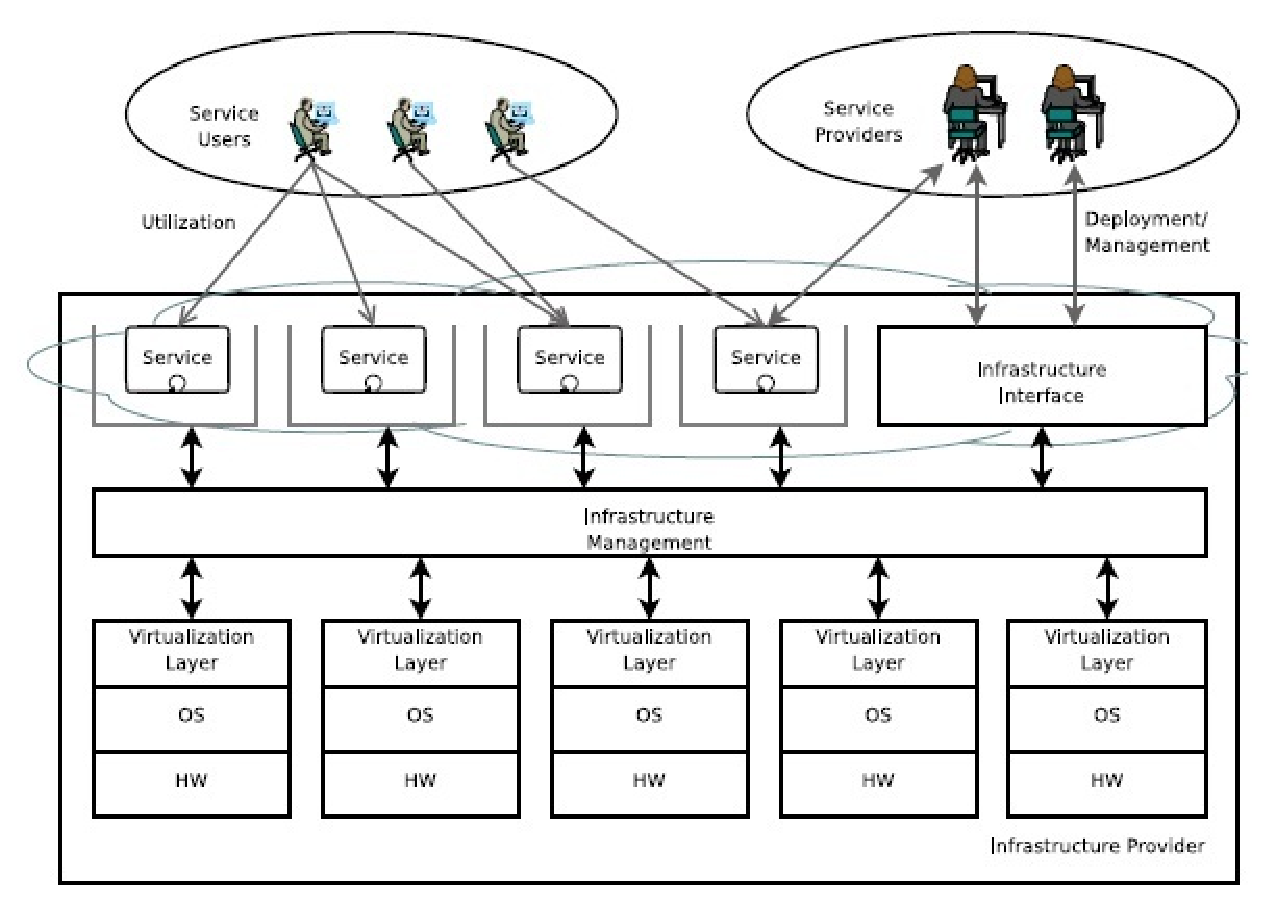
\includegraphics[scale=0.5]{Figures/actores}
  \caption{Actores en un sistema en la nube.}
  \label{act}
\end{figure}

\section{Comparaci�n entre servicios web y Grid computing/Cloud computing}

Como es sabido, nuestro grupo de investigaci�n ha centrado su investigaci�n en el desarrollo de una metodolog�a que permita construir y verificar sistemas con restricciones temporales mediante el uso de t�cnicas formales. En los �ltimos a�os, se ha aplicado esta metodolog�a en el �rea de los servicios web, m�s concretamente, en que estos servicios cumplan la tarea que se les encomienda y que se coordinen autom�ticamente para conseguir llevar a cabo un trabajo m�s general. El problema que est�n teniendo los servicios web es que como tuvieron un gran auge hace pocos a�os, muchos grupos de investigaci�n centraron sus estudios en este campo y, por tanto, hay muchos investigadores proponiendo nuevas aproximaciones y �sto ha llevado a que existen ciertas partes como BPEL o WS-CDL que est�n bastante estudiadas. De esta manera, esta surgiendo un sistema donde los m�todos formales pueden jugar un papel muy importante y donde nuestro grupo puede beneficiarse de su amplia experiencia tanto en formalizaci�n como en servicios web, el cloud computing. Este nuevo paradigma, como se ha expuesto anteriormente, est� viviendo su �poca de plenitud en este momento y grandes empresas como Google, IBM, Microsoft han decidido dar un paso al frente y apostar fuertemente por la computaci�n en la nube. Adem�s, muchos gobiernos est�n interesados en migrar sus servicios a la nube para abaratar costes y permitirles escalabilidad cuando les sea necesaria. Por ejemplo, hay que preguntarse si es necesario para la Agencia Tributaria tener grandes centros de datos cuando la demanda de servicios por parte de los ciudadanos s�lo crece en la �poca de la declaraci�n de la renta. Probablemente la respuesta sea afirmativa porque s� necesita almacenar todos esos datos y dar cierta confianza de que tus datos fiscales no van a caer en manos de gente con no muy buenas intenciones, pero toda la necesidad de c�lculo si que se puede externalizar para ahorrar costes en equipamiento o incluso podr�an crear una nube privada entre todos los organismos que colaboren con la agencia p�blica para compartir recursos e informaci�n. En este sentido, este tipo de sistemas donde la seguridad, privacidad y la disponibilidad son un requisito innegociable es donde podemos centrar parte de nuestras investigaciones e intentar mejorar alguno de los componentes de la arquitectura cloud expuesta en el apartado anterior. Por ejemplo, la mayor�a de grupos de investigaci�n desarrollan herramientas, pero la fase de pruebas o no existe o se le dedica poco tiempo. La semana pasada nos reunimos con uno de los grandes investigadores en el campo del Grid/Cloud Computing, Karim Djemame, y nos cont� que el principal problema que ten�a era ese que no sab�an concretamente porque funcionaba bien su herramienta y que estaba bastante interesado en la verificaci�n de su herramienta. \\


Por otro lado, a continuaci�n se enumeran algunas diferencias entre servicios web y grid/cloud computing para ver donde es posible aplicar nuestra experiencia en este sistema. En primer lugar, podemos considerar que los servicios web son en s� software que se ofrece como servicio (SaaS), aunque existan ciertas diferencias entre ambos enfoques, por ejemplo, la estandarizaci�n. Por tanto, este software podr�a estar compuesto de un conjunto de servicios, probablemente comunicados a trav�s de Internet, y que se coordinan para realizar una determinada tarea. Hasta el momento, nada nuevo, pero la principal diferencia reside en la virtualizaci�n, ya que los diferentes servicios que ofrece la nube se realizan en m�quinas virtuales en lugar de directamente sobre un servidor como puede ser el caso del servicio web, de manera que la concurrencia en el sistema es mayor. \\

Otra diferencia es la persistencia de los datos. Si queremos coordinar varios servicios web para que realicen sumas la �nica posibilidad de que �stos puedan almacenar el resultado es guard�ndolo en la base de datos, sin embargo, existe una aproximaci�n llamada WSRF (Web Services Resources Framework) que ha sido estandarizada y que resuelve este problema. En este framework cada servicio web lleva asociado un recurso o varios del sistema de manera que puedes interactuar con el servicio y decidir a que recurso acceder. La principal ventaja que tiene es que todos los servicios se definen con WSDL (Web Services Description Language) y que la comunicaci�n, direccionamiento, etc. est� estandarizado, de manera que la colaboraci�n entre sistemas de este tipo es sencilla. Otra ventaja es que el usuario tiene la posibilidad de decidir con que recursos interact�a. As�, podr�amos a�adir una capa inferior en nuestra metodolog�a que permitiese la definici�n de servicios web con recursos y una vez verificado que el sistema es correcto, desplegar estos servicios web en las m�quinas f�sicas. Este enfoque encajar�a perfectamente con nuestra investigaci�n, ya que utiliza servicios web con recursos y estos recursos tienen restricciones temporales para evitar que un usuario abarque todo el sistema. \\   

Tambi�n, podemos observar que cloud computing podr�a verse como una capa que se colocar�a debajo de los servicios web, ya que se puede utilizar �stos para acceder a los recursos, pero hay que resaltar que la nube no es solo ofrecer software como servicio, sino que tambi�n hay infraestructura y plataforma como servicio, cosa que los servicios web no pueden abarcar. Es decir, una parte del cloud computing (SaaS) puede compararse directamente con los servicios web, pero las otras dos partes no tienen nada que ver, por lo que ser�a como comparar el protocolo TCP/IP con la arquitectura de un PC, aunque es necesario que ambas aproximaciones (servicios web y cloud computing) converjan para el crecimiento de ambos paradigmas, igual que grid computing y servicios web convergieron en WSRF. \\

Por �ltimo, a modo de curiosidad la principal diferencia entre un sistema grid y uno cloud reside en la virtualizaci�n, ya que en grid el usuario no comparte en tiempo real los recursos que tiene asignados, mientras que en cloud es indispensable la virtualizaci�n de recursos para conseguir dar servicio a m�s clientes y conseguir ese ahorro que prometen los proveedores.

\section{Web Services Resource Framework(WSRF)}

La arquitectura que presentan los servicios web ha sido ampliamente aceptada como medio para estructurar las interacciones existentes entre los servicios que forman parte de un sistema distribuido y que colaborar para conseguir un objetivo com�n. En la actualidad, los desarrolladores requieren a los entornos una mayor estandarizaci�n para facilitar interoperatividad adicional entre dichos servicios, pero hasta mediados de 2004 ning�n grupo de investigaci�n o grupo de expertos se hab�a planteado seriamente la idea de proponer un est�ndar para modelar la comunicaci�n entre servicios web que poseen recursos persistentes asociados. As�, en Enero de ese a�o, varios miembros de la organizaci�n \emph{Globus Alliance} y de la multinacional inform�tica IBM definieron, con la ayuda de expertos de empresas como HP, SAP, Akamai, etc., la especificaci�n de los documentos que deber�an producirse en este modelo y la base de una arquitectura inicial. Estos documentos fueron enviados a la organizaci�n encargada de su estandarizaci�n, OASIS, en Marzo de 2004. En un principio, se formaron dos comit�s que se encargar�an del estudio y desarrollo de ciertas partes de este nuevo est�ndar. Por un lado, estaba el \emph{WSRF Technical Committee} que gestionaba cuatro especificaciones: \emph{WS-ResourceProperties, WS-ResourceLifetime, WS-ServiceGroup, y WS-BaseFaults}. Por otro lado, el \emph{WSN Technical Committee} se encargaba de las especificaciones: \emph{WS-BaseNotification, WS-Topics, y WS-BrokeredNotification}. \\

WS-Resource Framework est� inspirado en el trabajo realizado previamente por el \emph{Global Grid Forum's Open Grid Services Infrastructure (OGSI) Working Group} \cite{Foster03}. M�s concretamente, puede ser visto como una sencilla refactorizaci�n de los conceptos e interfaces desarrollados en la especificaci�n \emph{OGSI V1.0}, de manera que explota los recientes desarrollos en el �rea de los servicios web (por ejemplo, WS-Addressing). \\

El objetivo de este trabajo es introducir los conceptos fundamentales para la gesti�n y destrucci�n de servicios web persistentes, es decir, servicios web que llevan asociados recursos donde guardar los estados de los mismos, ya que hasta la aparici�n de esta aproximaci�n, los servicios web eran considerados ``\emph{stateless}'' y, por tanto, no pod�an almacenar temporalmente datos o resultados de sus operaciones de una manera sencilla para el usuario, ya que era necesario almacenarlos en una base de datos ajena al servicio. En este enfoque, es necesario codificar la relaci�n entre el servicio y el recurso en t�rminos de patrones utilizando una serie de tecnolog�as ampliamente estudiadas, como, por ejemplo, el WS-Addressing y, tambi�n, ser� necesario hacer sus propiedades accesibles desde el exterior a trav�s de un interfaz. En este sentido, llamaremos \emph{WS-Resource} a la asociaci�n entre un servicio web y un recurso persistente.  


\subsection{Introducci�n}

WS-Resource Framework \cite{Ban06} es una especificaci�n, desarrollada por OASIS y algunas de las empresas inform�ticas m�s pioneras, cuyo prop�sito es definir un marco gen�rico para el modelado y acceso a recursos asociados a servicios web, as� como las relaciones entre dichos recursos en un entorno Grid/Cloud. Esta aproximaci�n est� compuesta por un conjunto de especificaciones que definen la representaci�n del WS-Resource en los t�rminos que especifican los mensajes intercambiados y los documentos XML relacionados. Asimismo, incluye mecanismos que describen el medio para consultar el estado de un recurso y la descripci�n del servicio, que forman conjuntamente la definici�n de un WS-Resource. Adem�s, definen los pasos necesarios para hacer el estado de un servicio web accesible a trav�s de su interfaz (descrita en WSDL).\\

Normalmente, las interfaces de los servicios web proporcionan al usuario la posibilidad de acceder y manipular el estado del mismo, como, por ejemplo, valores de datos que evolucionan por la interacci�n entre varios servicios. En otras palabras, los intercambios de mensajes que se implementan en el comportamiento de los servicios tienen como objetivo permitir el acceso a estos recursos persistentes. Sin embargo, la noci�n de recursos persistentes que subyace en la implementaci�n de los servicios no es tan evidente en la definici�n de la interfaz \cite{Fost04}. Los mensajes que estos servicios env�an y reciben implican (o animan al programador a inferir) la existencia de un tipo de recurso asociado. Por tanto, es deseable que se definan est�ndares que permitan el descubrimiento, creaci�n, introspecci�n, interacci�n y destrucci�n de dichos recursos y que la forma elegida para llevar a cabo esta misi�n sea lo m�s interoperable posible. Estas observaciones han motivado la aparici�n de la propuesta comentada anteriormente, WS-Resource, para modelar estados en el contexto de los servicios web. Un WS-Resource se define como la composici�n de un servicio web y sus recursos persistentes asociados, esto es, \emph{(i)} expresado como una asociaci�n de un documento XML con un tipo definido con uno o varios \emph{portTypes} (un servicio podr� jugar un determinado rol si implementa todos los \emph{portTypes} que comprenden ese rol) y \emph{(ii)} direccionado y accedido de acuerdo al patr�n del recurso impl�cito, una derivaci�n de las \emph{Endpoint References} del WS-Addressing. Una \emph{Endpoint Reference} estar� compuesta por: Uniform Resource Identifier (URI), par�metros del mensaje que se envi� para solicitar el env�o de la \emph{Endpoint Reference} y datos relativos a la interfaz que se usa. En este intercambio, el identificador del recurso persistente es encapsulado en una \emph{Endpoint Reference} y usado para identificar al recurso en cualquier intercambio de mensajes entre los servicios que formen la coreograf�a. As�, WSRF permite declarar, acceder, monitorizar y destruir WS-Resources mediante mecanismos convencionales, lo que facilita la tarea de gesti�n, ya que no es necesario hacer m�s dif�cil la l�gica de decisi�n del servicio propietario del recurso para procesar los mensajes de gesti�n. Estos mecanismos convencionales componen cinco especificaciones t�cnicas que definen los medios por los cuales:

\begin{itemize}
\item Se destruye un WS-Resource, ya sea de manera s�ncrona con respecto a una petici�n expl�cita de destrucci�n o, a trav�s de un mecanismo basado en tiempos (scheduled). Adem�s, es posible declarar unas caracter�sticas espec�ficas  de los recursos (WS-ResourceProperties) que podr�an ser utilizadas para inspeccionar y monitorizar el tiempo de vida de dicho WS-Resource (WS-ResourceLifetime).
\item  Se definen los tipos de WS-Resource, que est�n compuestos por la interfaz de la descripci�n del servicio web (WSDL) y por un documento XML de propiedades del recurso. Por otro lado, el estado del WS-Resource puede ser consultado y modificado a trav�s del intercambio de mensajes (WS-ResourceProperties)
\item Un Endpoint Reference (WS-Addressing) puede ser renovado cuando su informaci�n de direccionamiento ha caducado o ha dejado de ser v�lida por alg�n error (WS-RenewableReferences).
\item Adem�s, se define la capacidad de implementar entornos heterog�neos como colecciones de servicios web, sean o no WS-Resources (WS-ServiceGroups).
\item La notificaci�n de errores puede ser m�s estandarizada al usar tipos XML Schema para definir los fallos base y definir reglas que muestren c�mo esos fallos son usados y extendidos (WS-BaseFaults).
\end{itemize}   

\subsection{WS-ResourceProperties}

Como se ha comentado anteriormente, WSRF utiliza una especificaci�n concreta para definir las propiedades del WS-Resource. Este recurso estar� compuesto por la definici�n de la interfaz en WSDL y un documento XML (Resource Properties Document) que especifica las propiedades del mismo, por ejemplo, el tama�o de disco, la capacidad del procesador, etc., de tal manera que si queremos acceder, modificar o actualizar este documento debemos utilizar una serie de mensajes preestablecidos en la especificaci�n. Las operaciones que se pueden hacer son las siguientes:

\subsubsection{GetResourceProperty}
Esta operaci�n como su propio nombre indica permite al servicio web que realiza la petici�n recuperar el valor de una {\bf �nica} propiedad del documento de propiedades. Para aclarar m�s los conceptos se define el siguiente ejemplo. \\


Dado el documento de propiedades:

\lstset{language=XML, numbersep=5pt,basicstyle=\small, frame=single}
\begin{lstlisting}
...
<GenericDiskDriveProperties 
xmlns: tns=``http://example.com/diskDrive'' >
  <tns:NumberOfBlocks>22</tns:NumberOfBlocks>
  <tns:BlockSize>1024</tns:BlockSize>
  <tns:Manufacturer>DrivesRUs</tns:Manufacturer>
</GenericDiskDriveProperties>
...
\end{lstlisting}

Una posible petici�n puede ser:

\lstset{language=XML, numbersep=5pt,basicstyle=\small, frame=single}
\begin{lstlisting}
...
<s12:Body>
  <wsrp:GetResourceProperty 
    xmlns:tns=``http://example.com/diskDrive''>
     tns:NumberOfBlocks
  </wsrp: GetResourceProperty>
</s12:Body>...
\end{lstlisting}

\subsubsection{GetMultipleResourceProperties}
Este m�todo es equivalente al anterior, pero para acceder a m�s de una propiedad del documento en el mismo mensaje, es decir, se utiliza para evitar congestionar la red. El mensaje enviado ser�a:


\lstset{language=XML, numbersep=5pt,basicstyle=\footnotesize ,frame=single}
\begin{lstlisting}
...
<wsrp:GetMultipleResourceProperties
 xmlns:tns=``http://example.com/diskdrive''>
 <wsrp:ResourceProperty>tns:NumberOfBlock</wsrp:ResourceProperty>
 <wsrp:ResourceProperty>tns:BlockSize</wsrp:ResourceProperty>
</wsrp:GetMultipleResourceProperties>
...
\end{lstlisting}

\subsubsection{SetResourceProperties}
Este m�todo se utiliza para realizar cambios en el documento de propiedades. Existen 3 tipos de cambios:

\begin{itemize}
\item Insert: Permite a�adir nuevas propiedades en el documento.
\item Update: Se utiliza para actualizar el valor de alguna propiedad.
\item Delete: Elimina propiedades del documento.
\end{itemize}

Un posible ejemplo de petici�n ser�a:

\lstset{language=XML, numbersep=5pt, basicstyle=\small,frame=single}
\begin{lstlisting}
...
<s12:Body>
 <wsrpw:SetResourceProperties
        xmlns:tns=``http://example.com/diskdrive''>
   <wsrp:Update>
    <tns:NumberOfBlocks>143</tns:NumberOfBlocks>
   </wsrp:Update>

   <wsrp:Delete resourceProperty=``tns:Manufacturer''/>

   <wsrp:Insert>
    <tns:someElement>42</tns:someElement>
   </wsrp:Insert>

 </wsrp:SetResourceProperties>
</s12:Body>
...
\end{lstlisting}


El documento de propiedades quedar�a con el siguiente formato:

\lstset{language=XML, numbersep=5pt, frame=single}
\begin{lstlisting}
...
<GenericDiskDriveProperties
  xmlns:tns=``http://example.com/diskDrive''>
  
  <tns:NumberOfBlocks>143</tns:NumberOfBlocks>
  <tns:BlockSize>1024</tns:BlockSize>
  <tns:someElement>42</tns:someElement>

</GenericDiskDriveProperties>
...
\end{lstlisting}

\subsubsection{QueryResourceProperties}
Como su propio nombre indica, este m�todo se utiliza para realizar consultas sobre propiedades del recurso. Por ejemplo si queremos saber si el n�mero de bloques es mayor que 20 y el tama�o de bloque es 1024 realizar�amos la siguiente consulta:

\lstset{language=XML, numbersep=5pt, frame=single}
\begin{lstlisting}
...
<s12:Body>
 <wsrp:QueryResourceProperties>
  <wsrp:QueryExpression
   Dialect=``http://www.w3.org/REC-xpath-19991116''>
    boolean(/*/NumberOfBlocks>20 and /*/BlockSize=1024)
  </wsrp:QueryExpression>
 </wsrp:QueryResourceProperties>
</s12:Body>
...
\end{lstlisting}

\newpage
La respuesta que env�a el otro servicio es:


\lstset{language=XML, numbersep=5pt, frame=single}
\begin{lstlisting}
...
<s12:Body>
 <wsrp:QueryResourcePropertiesResponse>
   true
 </wsrp:QueryResourcePropertiesResponse>
</s12:Body>
...
\end{lstlisting}


\subsection{WS-Base Faults}
El dise�ador de un servicio web normalmente utiliza interfaces definidas por otros, por lo que un m�todo que estandarizase el formato de los mensajes de notificaci�n de errores facilitar�a la labor de los desarrollares. �ste es el objetivo de WS-BaseFaults. Los mensajes de fallos en WSRF tienen el siguiente formato:


\lstset{language=XML, numbersep=5pt, frame=single}
\begin{lstlisting}
...
<BaseFault> 
  <Timestamp>xsd:dateTime</Timestamp> 
  <OriginatorReference> 
    wsa:EndpointReferenceType 
  </OriginatorReference> ? 
  <ErrorCode dialect=``anyURI''>xsd:string</ErrorCode>? 
  <Description>xsd:string</Description> * 
  <FaultCause>wsbf:BaseFault</FaultCause> * 
</BaseFault>
...
\end{lstlisting}
donde:

\begin{itemize}
\item Timestamp: Hora exacta cuando el fallo ha ocurrido.
\item OriginatorReference: Direcci�n en formato WS-Addressing del servicio que ha generado el fallo.
\item ErrorCode: C�digo de error para ser utilizado por sistemas de informaci�n de fallos, por ejemplo, POSIX errno.
\item Description: Explicaci�n de la causa del fallo (en lenguaje natural).
\item FaultCause: Causa t�cnica del fallo. 
\end{itemize}

\subsection{WS-ServiceGroup}
Esta especificaci�n permite crear grupos que comparten una serie de propiedades en com�n, es decir, agrupar diferentes servicios web que tienen comportamientos similares.

\subsection{WS-ResourceLifetime}

El tiempo de vida de un WS-Resource se define como el per�odo que transcurre entre su instanciaci�n y su destrucci�n. La misi�n de esta especificaci�n es estandarizar el proceso de destrucci�n de un recurso y definir mecanismos para monitorizar este ciclo de vida, pero lo que no se define es c�mo crear el WS-Resource. Generalmente, en los sistemas distribuidos, los clientes s�lo quieren tener un recurso por un determinado intervalo de tiempo, aunque en muchos escenarios es m�s apropiado para el cliente que se produzca la inmediata destrucci�n del recurso. Otro ejemplo claro de uso se presenta cuando el cliente quiere suscribirse a un servicio por un cierto tiempo y quiere que despu�s de este tiempo se destruya dicha uni�n. Como se coment� en la introducci�n, existen dos formas de destruir un recurso: inmediata, mediante un mensaje expl�cito o temporizada, mediante un mensaje que activa o gestiona un timer. 

\subsubsection{Destrucci�n inmediata}
Para la destrucci�n inmediata s�lo hace falta poner \emph{$<wsrl:Destroy/>$} dentro del cuerpo ($<Body>$) del mensaje SOAP que se env�a al servicio que gestiona el recurso y dicho servicio responder con \emph{$<wsrl:DestroyResponse/>$} dentro del cuerpo (\emph{$<Body>$}) del mensaje SOAP de respuesta.

\subsubsection{Destrucci�n temporizada}

En este caso, el WS-Resource tiene asociado un tiempo de terminaci�n que define el tiempo despu�s del cual se espera que el recurso haya sido destruido y, razonablemente, se espera que antes del mismo el recurso est� disponible. A continuaci�n se muestra un ejemplo de c�mo determinar el tiempo de terminaci�n de un recurso:

\lstset{language=XML, numbersep=5pt, frame=single}
\begin{lstlisting}
...
  <s12:Envelope
     <ex:ResourceDisambiguator>
      uuid:ba32-8680cace43f9
     </ex:ResourceDisambiguator>
     <s12:Body>
      <wsrl:SetTerminationTime>
       <wsrl:RequestedTerminationTime>
        2001-12-31T12:00:00
       </wsrl:RequestedTerminationTime>
     </wsrl:SetTerminationTime>
     </s12:Body>
  </s12:Envelope>
...
\end{lstlisting}



Como podemos observar el servicio que solicita la destrucci�n puede indicar la hora de destrucci�n y la hora actual (para evitar desajustes por la forma de representar la zona horaria). Una vez que CurrentTime alcanza el valor TerminationTime, el recurso se destruye sin ninguna intervenci�n m�s y se notifica al emisor del mensaje de destrucci�n que el recurso deja de estar disponible. Existe otro mensaje que se manda desde el receptor al emisor para comunicarle que ha recibido la petici�n de cambio.  \\

Sin embargo, puede darse la situaci�n de que haya m�s de un servicio utilizando el recurso que vaya a destruirse por lo que el propietario del recurso puede decidir o no (se deja a libre elecci�n del programador) implementar los mensajes WS-Notification para informar a los interesados que el recurso deja de estar disponible. Para llevar a cabo esta tarea debe crear este Topic: 

\newpage

\lstset{language=XML, numbersep=5pt, frame=single}
\begin{lstlisting}
...
<wstop:TopicSpace name=``ResourceLifetime''
   targetNamespace=
   http://docs.oasis-open.org/wsrf/2004/06/
   wsrf-WS-ResourceLifetime-1.2-draft-01.xsd
 
 <wstop:Topic name=``ResourceTermination''>
   <wstop:MessagePattern>
     <wsrp:QueryExpression
       dialect= http://www.w3.org/REC-xpath-19991116 >
        boolean(/*/TerminationNotification)
     </wsrp:QueryExpression>
 </wstop:MessagePattern>
...
\end{lstlisting}



Adem�s, el mensaje de notificaci�n asociado debe contener los siguientes campos: 


\lstset{language=XML, numbersep=5pt, frame=single}
\begin{lstlisting}
...
<wsrl:TerminationNotification>
 <wsrl:TerminationTime>xsd:dateTime</wsrl:TerminationTime>
 <wsrl:TerminationReason>xsd:any</wsrl:TerminationReason>?
</wsrl:TerminationNotification>
...
\end{lstlisting}
 
donde \emph{TerminationTime} informa de la fecha de destrucci�n y \emph{TerminationReason} contiene la explicaci�n de la destrucci�n.

\section{WS-Notification}

Esta especificaci�n permite a un \emph{NotificationProducer} enviar un mensaje de notificaci�n a un \emph{NotificationConsumer} de dos maneras diferentes:

\begin{enumerate}
\item El \emph{NotificationProducer} env�a un mensaje de notificaci�n al \emph{NotificationConsumer} sin seguir ning�n formalismo.
\item El \emph{NotificationProducer} utiliza el formalismo que se describe a continuaci�n para enviar las notificaciones. 
\end{enumerate} 

La opci�n a utilizar la elegir� el suscriptor cuando mande la petici�n de suscripci�n. En este sentido, la segunda opci�n permite al usuario recibir un amplio rango de mensajes de notificaci�n, ya que la informaci�n que se env�a en estos mensajes se obtiene de un �rbol de Topics (temas) y, por tanto, se permite enviar sub�rboles en un mismo mensaje para informar de diferentes Topics. En la Figura \ref{12} vemos un ejemplo:


\begin{figure}[h!]
  \center
    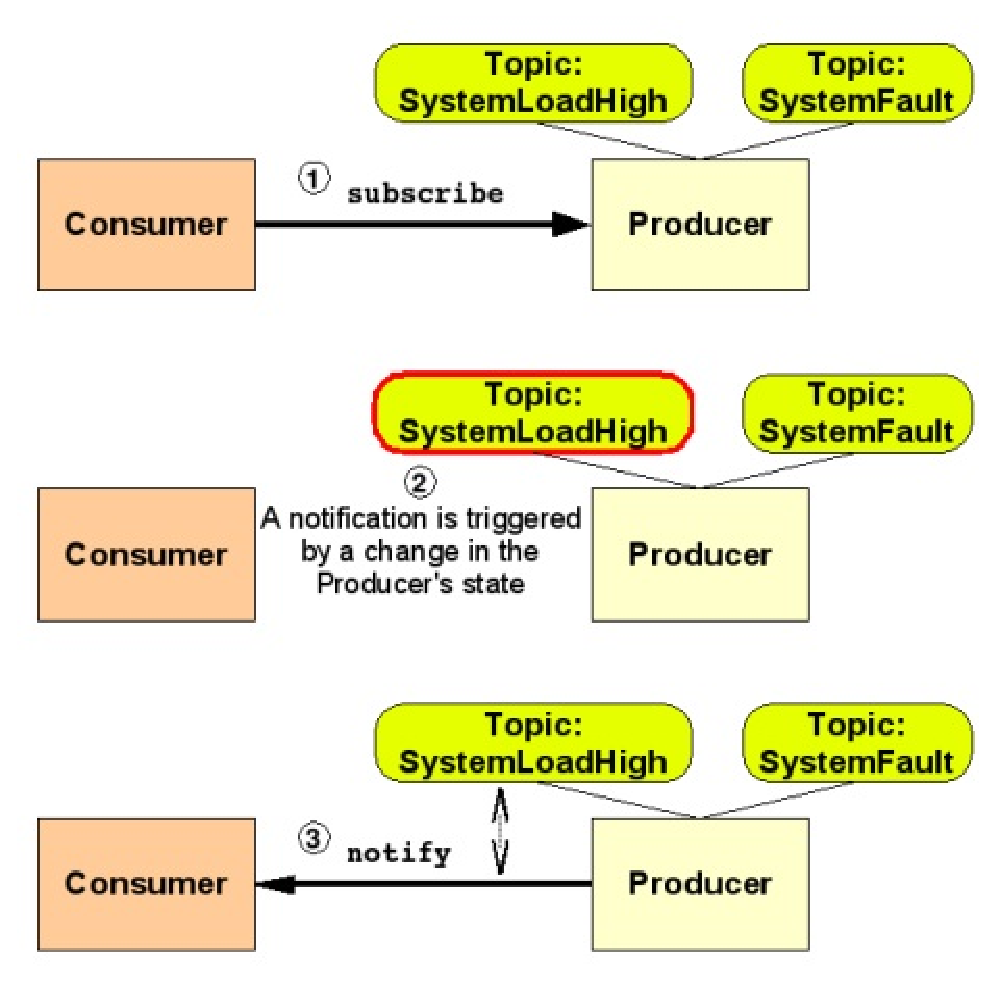
\includegraphics[scale=0.45]{Figures/12}
     \caption{Ejemplo de uso de WS-Notification sin broker.}
  \label{12}
\end{figure}
 
Este caso muestra un ejemplo de interacci�n entre un consumidor y un productor de notificaciones, en el caso de que el suscriptor y el consumidor sean la misma entidad. El sistema es simple ya que tenemos un consumidor y un productor que publica 2 topics: SystemLoadHigh y SystemFault. Los pasos necesarios son: 

\begin{enumerate}
\item En primer lugar, el consumidor se suscribe al topic SystemLoadHigh, por lo que internamente se crea un \emph{Subscription resource} con la informaci�n de la suscripci�n. El productor debe implementar un m�todo \emph{Subscribe} y el consumidor un m�todo \emph{Notify}.  
\item Despu�s, el productor debe enviar una notificaci�n cuando el sistema sobrepase una determinada carga de trabajo. Por ejemplo, nuestro sistema enviar� notificaciones cuando la carga de trabajo sea mayor de 50\%.
\item Por �ltimo, el productor env�a la notificaci�n invocando la operaci�n \emph{Notify} en el consumidor.
\end{enumerate}
   
Un ejemplo de mensaje \emph{Notify} es:
 
\lstset{language=XML, numbersep=5pt, frame=single}
\begin{lstlisting}
...
<wsnt:Notify>
    <wsntw:NotificationMessage>
     <wsnt:Topic Dialect= xsd:anyURI >
       {any}
     </wsnt:Topic>
     <wsnt:ProducerReference>?
      wsa:EndpointReference
     </wsnt:ProducerReference>
     <wsnt:Message>xsd:any</wsnt:Message>
    <wsnt:NotificationMessage>+
</wsnt:Notify>
...
\end{lstlisting}

Como podemos observar el mensaje \emph{Notify} contiene uno o varios mensajes de notificaci�n (\emph{NotificationMessages}). Los campos dentro de �stos son: 

\begin{itemize}
\item Topic: La informaci�n del topic que se env�a.
\item Dialect: El dialecto usado para expresar el topic anterior, es decir, el lenguaje utilizado para expresarlo.
\item ProducerReference: Direcci�n del productor.
\item Message: Una copia de la carga �til (payload) del mensaje actual.
\end{itemize}

A continuaci�n, se muestra el mensaje que manda el suscriptor para registrar su inter�s en uno o m�s topics:


\lstset{language=XML, numbersep=5pt, frame=single}
\begin{lstlisting}
...
<wsnt:Subscribe>
  <wsnt:ConsumerReference>
    wsa:endpointReference
  </wsnt: ConsumerReference>
  <wsnt:TopicExpression Dialect = xsd:anyURI >
    {any}
  </wsnt:TopicExpression>
  <wsnt:UseNotify>xsd:boolean</wsnt:UseNotify>?
  <wsnt:Precondition>wsrp:QueryExpression</Precondition>?
  <wsnt:Selector>wsrp:QueryExpression</wsnt:Selector>?
  <wsnt:SubscriptionPolicy>{any}</wsnt:SubscriptionPolicy>?
  <wsnt:InitialTerminationTime>
    xsd:dateTime
  </wsnt:InitialTerminationTime>?
</wsnt:Subscribe>

...
\end{lstlisting}


Los conceptos importantes en este mensaje son \emph{UseNotify} que se utiliza para decidir si el mensaje de notificaci�n sigue el formalismo WS-Notification o se manda sin formato, \emph{Precondition} que es la condici�n que genera mensajes de notificaci�n, es decir, si se cumple esta condici�n se generan mensajes, pero debe cumplirse tambi�n la condici�n \emph{selector} para enviarlos a los destinatarios que es la que se usa para decidir si se transmiten o no los mensajes generados. Adem�s, \emph{SubscriptionPolicy} se podr�a utilizar para controlar el ratio de env�o de mensajes(por ejemplo, no m�s de 3 por segundo) y \emph{InitialTerminationTime} contiene una sugerencia del tiempo de vida de la suscripci�n. WSRF tambi�n incluye mensajes para detener la suscripci�n, reanudarla o para que un servicio que acaba de unirse a una suscripci�n pueda obtener un historial de notificaciones sobre un determinado topic.



\subsection{WS-BrokeredNotification}

Un \emph{NotificationBroker} es un intermediario que, entre otras cosas, permite el env�o de mensajes entre uno o varios \emph{Publishers} y uno o varios \emph{NotificationConsumers}. La misi�n del \emph{Publisher} es observar ciertas situaciones y crear mensajes de notificaci�n para informar de esas situaciones, mientras que el broker es el encargado de distribuir estos mensajes. \\

En este caso, se pueden dar tres relaciones entre las partes: \emph{simple publishing}, \emph{composable publishing} y \emph{demand-based publishing}. En el primer caso, el \emph{Publisher} es el encargado de observar las situaciones y notificarlas al broker que ser� el encargado de transmitirlas a los interesados. En el segundo caso, el papel del \emph{Publisher} lo realizar� una entidad que implementa una serie de servicios especificados en WS-Notification (NotificationProducer). En este caso, el mensaje de notificaci�n puede llegar a otros consumidores que estuviesen suscritos al productor. En ambos casos, el broker puede pedir al \emph{Publisher} que se registre para poder publicar mensajes sobre un topic determinado. El �ltimo enfoque (\emph{demand-based publishing}) requiere que el \emph{Publisher} sea un \emph{NotificationProducer} y, as�, acepte mensajes de suscripci�n. El objetivo es reducir el n�mero de mensajes de notificaci�n haciendo que �stos solo se manden cuando se soliciten expresamente.


\cleardoublepage

\chapter{BPELRF}\label{chapter:c3}
\markboth{Chapter~\ref{chapter:c3}. Design and Verification of Web Service Compositions}{}
%
%This chapter presents a methodology called \textit{Correct-WS} for the creation of correct Web Service compositions including time constraints. Some of the model translations needed among the different phases of this methodology are described in detail and a tool that we have developed to automate these translations of the methodology is also introduced. Next, a case study showing a Web Service composition for an Internet purchase process is presented, where the tool is applied for the development of a correct composition. Finally, the remaining translations of the methodology and other parallel works are briefly referenced.
%
\section{Introduction}
The development of software systems is becoming more complex with the 
appearance
of new computational paradigms such as Service-Oriented  Computing  (SOC), 
Grid Computing and Cloud Computing. Grid/Cloud environments are characterized by a dynamic environment due to the heterogeneity and volatility of resources. In these systems, the service provider needs to ensure some levels of 
quality and privacy to the final
user in a way that had never been raised. It is therefore necessary to develop new techniques to benefit from the advantages 
of recent approaches, such as Web service compositions. %Formal models of concurrency have been widely used for the description and analysis of concurrent and distributed systems. SI LO PONGO SERIA CON CITAS
 There are two complementary views to composite Web services: Choreography and Orchestration. The choreography view describes the observable interactions among services and it can
be  defined  by  using  specific  languages such as Web  Services
Choreography  Description  Language  (WS-CDL) %\cite{WSCDL}
or  by using more general languages like UML Messages Sequence
Charts (MSC). On the other hand, orchestration concerns
the internal behaviour of a Web service in terms of invocations
to  other  services.  Web Services Business Process Execution Language (WS-BPEL) \cite{BPEL4WS} is in general used 
to describe Web service orchestrations, and, consequently, this
is considered the de-facto standard language for describing Web services
in terms of Web service compositions.

In addition, complex Web systems are composed by smaller services where each one carries out different tasks. Thus, to model such systems, specification languages should offer designers the constructions required to compose and discovery those basic services. Web service compositions could be modelled by using one of the two standards previously presented (WS-CDL or WS-BPEL). Service discovery is the process of finding a suitable Web service for a given task, and, normally, its definition is implementation-dependent. %In this work, we have formalised some constructions to represent the discovery and composition of services.

While Web service implementations are typically stateless, 
their interfaces frequently provide users with the ability
to access and manipulate states, i.e., data values that persist
across, and evolve as a result of Web service interactions. In
other words, the message exchanges that Web services implement
are frequently intended to enable access to stateful
resources. Besides, the messages that the services send
and receive imply (or programmers infer) the existence of
an associated resource type. Therefore, it is desirable to define Web
service conventions to enable the discovery of, introspection on, 
and interaction with stateful resources in standard
and interoperable ways. Most important, such an approach
improves the robustness of design time selection of services
during application assembly, and runtime binding to specific
resource instances \cite{Czajkowski2004}.
%This commonality of purpose
%has motivated the Open Grid Services Architecture
%to identify state modeling and
%management as a fundamental requirement for
%service-oriented architectures.
%Such considerations have led to the development
%of four specifications known collectively as the Web
%Services Resource Framework (WSRF [2]) which
%define conventional interfaces and behaviors for
%representing, abstracting, and manipulating state in a
%Web services framework. Three related WS-
%Notification 
%specifications define interfaces
%and behaviours that allow clients to subscribe to
%changes in state, thus providing for push-mode access
%to state components.
To facilitate additional interoperability among services, more standardization is required to deal with distributed resources. In January of 2004, several members of the \emph{Globus Alliance} organization and the computer multinational \emph{IBM} with the help of experts from companies such as \emph{HP, SAP, Akamai, etc.} defined the basis architecture and the initial specification documents of a new standard for that purpose, Web Services Resource Framework (WSRF)~\cite{Foster2004}.

Likewise, it is important to define a mechanism to state how the users are notified when important situations occur. To this end, a publish/subscribe architecture might be implemented, which is based on information preferences expressed in advance. Thus, whenever new content is available on one resource, the publisher would send that information to the subscriber. As far as this work is concerned, services might express its disposition to receive notifications when certain conditions hold. As WSRF specifications encourage, the present work utilizes WS-Notification as basis to cope with publish-subscribe architecture.

After introducing the relevant concepts, let us remark the main contributions of this work. The integration of WS-BPEL and WSRF is not new, since, in the literature, one can find some works defining this integration from a technical point of view. Some of these works will be presented in the Related Work section. Surprisingly, to the best of our knowledge, this is the first work, which taking as a starting point WSRF and WS-BPEL, defines a complete and formal language to model and analyse stateful Web service compositions. In addition to this, the necessary formal machinery to build a publish-subscribe architecture is also provided here improving the expressiveness of the language, and a formal primitive to discover new services is defined. It is worthwhile to mention that the aim of this paper is not to provide yet another WS-BPEL semantics since WS-BPEL has received much attention in recent years when many operational semantics for it have arisen. As opposed to this, the main aim here is to gather the benefits of putting together WS-BPEL and WSRF to manage stateful Web services workflows by using existing formalisms in distributed systems. Additionally, in order to deal with WSRF in a proper way, we have realised that it would be better to consider a semantic model with the appropriate ``tools'' to cope with all the relevant aspects of WSRF such as notifications and resources time-outs. To particularise and motivate our approach, we introduce now an ideal scenario.
The scenario, where our approach might be applicable, is a \textsl{group buying}, also known as collective buying.
This scenario consists of a group of sellers and buyers, where offers are interpreted as resources created by sellers. Buyers subscribe to those offers, and they are notified when the offers/resources
meet their expectations. This simple scenario will allow us to show readers how the situation can be managed
with what we consider a very simple and succinct language.
The rest of the paper is organised as follows. In Section \ref{rWork}, we present the basic concepts for a better understanding of this paper and some related works. In Section \ref{ops}, we define the language itself and its operational semantics, whereas, in Section \ref{cs}, we illustrate by means of a case study how it works. Finally, Section \ref{conclusions} presents some conclusions and possible future directions to improve the present work.

\section{Background and Related Work}\label{rWork}

{\bf Overview of BPEL/WSRF.} WSRF~\cite{Banks2006} is a resource specification language developed by OASIS and some of the most pioneering computer companies, whose purpose is to define a generic framework for modelling Web services with stateful resources (WS-Resource), as well as the relationships among these services in a Grid/Cloud environment. This approach consists of a set of specifications that define the representation of the WS-Resource in the terms that specify the messages exchanged and the related XML documents. These specifications allow the programmer to declare and implement the association between a service and one or more resources. It also includes mechanisms to describe the means to check the status and the service description of a resource, which together form the definition of a WS-Resource. This WS-Resource is accessible through its unique identifier, 
\emph{EndPoint Reference (EPR)}, which is defined by using WS-Addressing.

On the other hand, Web services are becoming more and more important as a platform
for Business-to-Business integration.  Web service compositions have appeared
as a natural and elegant way to provide new value-added services
as a combination of several established Web services.
Services provided by different suppliers can act together
to provide another service; in fact, they can be written in different
languages and can be executed on different platforms. As we noticed in the introduction, we can use Web service compositions as a way to construct Web service systems where each service is an autonomous entity which can offer a series of operations to the other services conforming a whole system. In this way, it is fairly necessary to establish a consistent manner to coordinate the system participants since each of them may use a different approach, and, consequently, it is common to use specific languages such as WS-BPEL to manage the system workflow. WS-BPEL, for short BPEL, is an OASIS orchestration language to specify actions within Web service business processes. These actions are represented by the execution of two types of activities (\emph{basic} and \emph{structured}) that perform the process logic. \emph{Basic activities} are those which describe elemental steps of the process behaviour and \emph{structured activities} encode control-flow logic, and can therefore contain other basic and/or structured activities recursively~\cite{BPEL4WS}.

The WSRF elements considered in our language are\footnote{In WSRF there are some additional technical elements to 
increase the modelling
power that due to its technical nature
are not considered in our framework.}:

\begin{itemize}
\item {\bf WS-ResourceProperties}: There is a explicit specification 
to define WS-Resource properties, based on 
a Resource Properties Document (RPD),  which
defines the properties of the associated resource
(disk size, processor capacity, etc.).
Nevertheless, for simplicity, we only consider a single property
for each resource, which is an integer value.
Among the operations allowed by the standard are \linebreak
\emph{GetResourceProperty} 
and \emph{SetResourceProperty}, which are used to manipulate 
the resource property values.
%
%The developer 
%typically uses a Web service interface defined by others, so a 
%method to standardise the format for reporting error messages 
%facilitates the work.
%
%
\item {\bf WS-ResourceLifetime}: The WSRF specification does not 
provide a standard way to create resources. However,
resources have an associated lifetime, which means that once
this time has elapsed, the resource is considered to be destroyed,
and the subscribers are correspondingly notified.
%
We have then included, for completeness, an operation to publish
resources, {\em publishResource}, in which the initial value
of the resource, its lifetime, a textual identifier in order to allow
users to discover it, and the activity that must
be launched upon its destruction are indicated. We also have
an operation in order to modify the current resource lifetime,
{\em setTimeout}. 

\item {\bf WS-Notification}: Clients can subscribe to WSRF
resources in order to be notified about some topics (resource
conditions). We therefore include the {\em subscribe} operator 
for a customer to subscribe to a resource, indicating the
condition under which it must be notified, and the activity that
must be executed 
upon that event.


\end{itemize}

{\bf Related Work.} WS-BPEL has been extensively studied with many formalisms, such as
Petri nets, Finite State Machines and process algebras, but
there are only a few works considering WS-BPEL enriched with
WSRF, and they only show a description of this union,
without a formalization of the model.
In \cite{Slomiski:2006} Slomiski uses BPEL4WS in Grid environments and discusses the
benefits and challenges of extensibility in the particular case of OGSI workflows
combined with WSRF-based Grids. Other two works centered around Grid environments are
\cite{Leymann:2006} and \cite{Ezenwoye:2007}. The first justifies
the use of BPEL extensibility to allow the combination of different GRIDs, whereas
Ezenwoye et al.~\cite{Ezenwoye:2007} share their experience on BPEL to integrate,
create and manage WS-Resources that implement the factory/instance pattern.

On the other hand, Ouyang et al. \cite{Ouyang:2007} define the necessary elements for translating BPEL processes into Petri nets. Thus, they
cover all the important aspects in the standard such as exception handling, dead path elimination and so on. The model they consider differs from ours in that we formalize the whole
system as a composition of orchestrators with resources associated, whereas they describe the system as a general scope with nested sub-scopes leaving aside the possibility of administering resources. Furthermore, we have also formalized the event handling and notification mechanisms.
Another extensive semantics for BPEL 2.0
is presented in \cite{Dumas:2008} by Dumas et al, which introduces two new interesting improvements. They define several patterns to simplify some huge nets and introduce the semantics for the WS-BPEL 2.0 new patterns. Related to $\pi$-calculus semantics, Dragoni and Mazzara \cite{Dragoni:2009}
propose a theoretical scheme focused on dependable composition for the  WS-BPEL recovery
framework. In this approach, the recovery framework is simplified
and analysed via a conservative extension of $\pi$-calculus. The
aim of this approach clearly differs from ours, but it helps us to have
a better understanding of the WS-BPEL recovery framework. Other work focused on the BPEL
recovery framework is \cite{Qiu:2005}. Although this is more focused in the compensation handler, they describe the corresponding rules
that manage a Web service composition. Our work is therefore quite complete as we define rules for nearly all possible activities. In addition, we also consider time constraints. Finally, we would like to highlight the works of Farahbod et al.~\cite{Farahbod:2005} and Busi et al. \cite{Busi:2005}. In the first one, the authors extract an abstract operational semantics for BPEL based on abstract state machines (ASM) defining the framework BPEL$_{AM}$ to manage the agents who perform the workflow activities. In this approach time constraints are considered, but they do not formalize the timed model. On the other hand, the goal of the latter one is fairly similar to ours. They also define a $\pi$-calculus operational semantics for BPEL and describe a conformance notion. They present all the machinery to model Web service compositions (choreographies and orchestrations). The main difference with our work is that we deal with distributed resources. In a similar fashion Luchi and Mazzara in \cite{Lucchi07} presents other $\pi$-calculus operational semantic, \textit{web}$\pi_{\infty}$, which is centred on the idea of event notification as the unique error handling mechanism. It is clear that this proposal differs from ours since they focus their attention in the error handling mechanism, however their claiming of simplifying the error handling using only the notification mechanism can be performed in our proposal since this is the mechanism used in the resource framework and therefore a technique shared by WS-BPEL and WS-RF.
% % % % DESDE AQUI HE CORTADOOOOOOOOOOOOOOOOOOOOOO
For further details about the formalization of service oriented languages we would like to encourage the reader to review the works presented at the SENSORIA project in \cite{Wirsing2011bis}. Here, an extensive work is presented from different international research groups aimed by the common goal of providing a rigorous software engineering view point for service-oriented system using as a cornerstone the formal specification of Web Services and WS-BPEL in particular. Works such as SOCK \cite{Wirsing2011bis}, CaSPiS \cite{Bettini2008}, COWS \cite{Lapadula2007}, B-lite \cite{Lapadula2008} or Orc \cite{Kitchin2009} are either presented or reviewed. The first one, SOCK (Service Oriented Computing Kernel \cite{Wirsing2011bis}), is a formal calculus which aims at characterizing the basic features of Service Oriented Computing and takes its inspiration from WS-BPEL, considered by the authors as the ``de facto" standard for Web Service technology. The second one, CaSPiS (Calculus of Services with Pipelines and Sessions \cite{Bettini2008}) uses the Java framework IMC. Authors take advantage of the already built-in IMC features such us session oriented and pattern matching communication mechanisms easing the task of implementing in Java all CaSPiS abstractions. Other one, COWS (Calculus for Orchestration of Web Services \cite{Lapadula2007}), is a new foundational language for SOC whose design has been influenced by WS-BPEL. COWS combines a number of elements from process calculi, e.g. asynchronous communication, polyadic synchronization, pattern matching, protection, delimited receiving and killing activities. 
%Other one reviewed also in this book is B lite \cite{Lapadula2008}. This is a lightweight language for web services orchestration designed around some of WS-BPEL peculiar features like partner links, process termination, message correlation, long-running business transactions and compensation handlers aiding to clarify some ambiguous aspects of the WS-BPEL specification. The last one, Orc \cite{Kitchin2009}, is not influenced by any other language used for orchestration purposes like WS-BPEL. The authors define the language as a novel language for distributed and concurrent programming which provides uniform access to computational services, including distributed communication and data manipulation, through sites. Using four simple concurrency primitives, the programmer orchestrates the invocation of sites to achieve a goal, while managing timeouts, priorities, and failures. This language uses as a basic activity the information published by a site and therefore each site invocation always finishes with one or more either nested or parallel publications.

\section{Syntax and semantics of BPEL+RF}\label{ops}
We use the following notation: {\it ORCH} is the set of orchestrators in the system, {\it VAR} is the set of integer variable names, {\it PL} is the set of necessary partnerlinks, {\it OPS} is the set of operations names that can be performed, {\it EPRS} is the set of resource identifiers (${\it EPRS\subseteq\nat}$), and {\it A} is the set of basic or structured activities that can form the body of a process. The specific algebraic language that we use
for the activities is defined by the following BNF-notation:
%
\[\begin{array}{l}
  A ::=  {\it throw} \;|\;           % go to the exception block
         {\it receive}(pl,op,v) \;|\;  % receive basic activity,
         {\it invoke}(pl,op,v_1) \;|\;
         {\it exit}\;|\;
         {\it reply}(pl,op,v)\;|\;\\  % reply basic activity
         {\it \overline{reply}(pl,op,v_2)}\;|\;
         {\it assign}(expr,v_1) \;|\;
                %~~~~~~~
         {\it empty}\;|\;
         \,\,A \,; A \,\, \;|\, % Sequence
         \;A \,\| \, A \;\,|\,   % parallel
         {\it while}(cond,A)\;|\ \\
         {\it wait}(timeout)\hspace{-0.1cm}\;|\;
         {\it pick}(\{(pl_i,op_i,v_i,A_i)\}_{i=1}^n,A,timeout)\;|\;
         {\it getProp}(vEPR,v_1)\hspace{-0.1cm}\;|\;\\
         {\it getTimeout}(vEPR,v_1)\;|\;
         {\it publishResource}(O,val,timeout,tag,vEPR,A)\;|\;
         {\it discover}(tag,vEPR)\;|\;\\
         {\it setProp}(vEPR,expr)\;|\;
         {\it setTimeout}(vEPR,timeout)\;|\;
         {\it subscribe}(O,vEPR,cond',A)
\end{array}
\]

 \hspace{0.4cm}where ${\it O \in ORCH, pl,pl_{i} \in PL, op,op_{i}}$ ${\it \in OPS, timeout \in \nat}$, {\it  expr} is an arithmetic expression constructed by using the variables in {\it VAR} and integers; ${\it v,v_1,v_2,v_i}$ range over {\it VAR}, {\it tag} is a string used to identify and discover resources that match a certain pattern, and $val \in \entero$. A variable $vEPR$ is used to store temporarily the resource identifier ({\it EPR}). A condition {\it cond} is a predicate constructed by using conjunctions, disjunctions, and negations over the set of variables {\it VAR} and integers, whereas {\it cond'} is a predicate constructed by using the variable {\it vEPR}, as representative of the resource value, and integers. \\%When in a condition or in an expression appears the variable {\it vEPR}, we suppose that the evaluation of this variable is not the resource identifier, but the value of this resource.\\
%Notice that \emph{getProp} contains a parameter {\it prop}, $prop \in \{\textrm{``value'',``timeout''}\}$, in order to distinguish between the two properties of the resource (its value and its termination time). On the contrary, the activity \emph{setProp} does not contain such a property since, as the WSRF specification says, the only way to change the termination time is by using the activity \emph{setTimeout}.
%We therefore use its EPR as representative of this property, as
%we already observed in the introduction.
BPEL basic activities leveraged in our model are: \emph{invoke} to request services offered by service providers, \emph{receive} and \emph{reply} to provide services to partners, \emph{throw} to signal an internal fault explicitly, \emph{wait} to specify a delay, \emph{empty} to do nothing, \emph{exit} to end the business process and \emph{assign}, which is used to assign a variable value. The \emph{structured activities} are: \emph{sequence} (represented here as ;), which contains two activities that are performed sequentially, \emph{while} to provide a (conditional) repeated execution of one activity, \emph{pick} that waits for the occurrence of exactly one event from a set of events (including an alarm event) executing then the activity associated with that event, and, finally, \emph{flow} ($\|$ operator in our syntax) to express concurrency. Another family of control flow constructs in BPEL includes event, fault and compensation handlers. An event handler is enabled when
its associated event occurs, being executed concurrently with the main orchestrator activity. Fault handlers are performed when some failure has occurred, so the control is transferred to them. In this work, we only cover the fault and event handling, leaving compensation as a matter of future research. Besides, we do not take into consideration other advanced constructions such as correlation sets, dynamic partnerlinks or instance creation. However, an important aspect in current services technology is that of publishing and discovering of resources, which is considered in our framework. The correspondence among the syntax of WS-BPEL, WSRF, WS-Notification and our model is shown in Table \ref{BPELsyntax}.
%ell as with the inclusion of structured variables, instead of just considering
%all variables as integers.
An orchestration is here defined as a pair ${\it O= (A,A_f)}$, where $A$ and $A_f$ are activities defined by the previous syntax. Specifically, $A$ represents the normal workflow (and possible event handling activities which run in parallel with it), and $A_f$ is the orchestrator fault handling activity.

Before we begin, we introduce some notations and definitions needed to describe the operational semantics.
\begin{definition}[State] %\label{states}
We define a state as a pair s=($\sigma, \rho$), where $\sigma$ represents the variable values in the system and $\rho$ captures the global resource state. We characterise $\sigma$ as a global function in ${\it \entero^\textrm{VAR}}$, but, in practice, each orchestrator will manage its own local variables. Furthermore, $\it{ \rho=\{(O_i,EPR_i,v_i,Subs_i,}$ $\it{ t_i,tag_i,A_{e{_i}})\}_{i=1}^r}$, where $r$ is the number of resources in the system. Each resource has an owner (publisher), ${\it O_i}$, a unique identifier, ${\it EPR_i}$, and, at each state, a particular value, $v_i$, and a lifetime, $t_i$, initialized with the activity {\it publishResource}, which can be changed by using the function {\it setTimeout}. $A_{e{_i}}$ is the activity that must be run when it expires, whereas ${\it tag_i}$ is used as a textual description for discovery purposes. The resources in $\rho$ are therefore published by means of the {\em publishResource} activity, and potential subscribers must discover the resource identifier (EPR) by using the {\it discover} activity. %This identifier will be stored temporarily in a variable $v$ that will be used to access such a resource.  %whereas the resource information ($\rho$) will be shared by all the orchestrators, i.e., any change introduced in $\rho$ by any orchestrator will be visible to others.
Moreover, $\it{Subs_i=\{(O_{i_{j}},cond'_{i_{j}},A_{e{_{_i{_{_j}}}}})\}_{j=1}^{{s_i}}}$, $i \in \{1,...,r\}$, is the set of resource subscribers, their associated delivery conditions and the event handling activity ${\it A_{e{_{_i{_{_j}}}}}}$ that must be thrown in the case that ${\it cond'_{i_{j}}}$ holds; $s_i$ is the number of orchestrators currently subscribed to this resource and ${\it O_{i_{j}} \in ORCH}$ are the subscriber identifiers.
\end{definition}

{\bf Notation.} Along the following lines, we introduce some notation used in the operational semantics. Given a state $s=(\sigma,\rho)$, a variable $v$ and an expression $e$, we denote by $s'=(\sigma[e/v],\rho)$ the state obtained from $s$
by changing the value of $v$ for the evaluation of $e$, and ${\it s{^+}=(\sigma,\rho')}$, where ${\it \rho'=\{(O_i,EPR_i,v_i,Subs_i,t_i-1,tag_i,A_{e{_i}})|}$ ${\it t_i>1\}_{i=1}^r}$. Let the function {\it Subs(s)}, which return the state {\it s} removing from each ${\it Subs_i}$ those subscriptions whose associated condition has held at {\it s}. %, then $s''=s' \setminus Subs(N(O,s))$, being the operator $\setminus$ the typical set subtraction operator. Note that this function avoids infinite executions over the same subscription even though a service could subscribe again with the same condition. 
We omit its formal definition since it is straightforward.

A partnerlink is here considered as a pair $(O_i,O_j)$ representing the two roles in communication: sender and receiver. Furthermore, $\it{\sigma(vEPR_i) \in \rho}$ and $\it{tag_i \in \rho}$ will denote that there is a tuple $\it{(O_i,EPR_i,}$ ${\it v_i,Subs_i,t_i,tag_i,A_{e{_i}}) \in \rho}$, where $\it{\sigma(vEPR_i)=EPR_i}$. Given a predicate $\it{cond}$, we use the function $\it{cond(s)}$ to mean the resulting value of this predicate at the current state {\it s}, {\it $sel(\rho,tag)$} to return a randomly selected ${\it EPR \in \rho}$ among those whose tag attribute is {\em tag} , ${\it val(\rho,tag)}$ to return the current value of the resource, ${\it time(\rho,vEPR)}$ to return its lifetime and, finally, {\it getEPR()} to generate non-repeated resource identifiers. Let ${\it \sigma(vEPR)=EPR}$, ${\it \rho[w/vEPR]_1}$ is used to denote that the new value in $\rho$ of the resource $\it{EPR}$ is $\it{w}$, $\it{\rho[t/vEPR]_2}$ denotes a change of the resource lifetime, and the function $\it{Add\_subs(\rho,vEPR_i,O_{i_{j}},cond'_{i_{j}},A_{e{_i{_{_j}}}})}$ denotes that $\it{(O_{i_{j}},cond'_{i_{j}},A_{e{_i{_{_j}}}})}$ is added to the subscribers of the resource $\it{EPR_i \in \rho}$ or ${\it cond'=cond'_{i_{j}}}$ in the case that $\it{O_{i_{j}}}$ was already in ${\it Subs_i}$.
At the same time, we need an additional function to launch the corresponding activities %in parallel with the normal workflow
when the subscriber condition holds at the current state ${\it s}$. Let s=($\sigma, \rho$) with $\it{ \rho=\{(O,EPR_i,v_i,Subs_i,t_i,tag_i,A_{e{_i}})\}_{i=1}^r}$, we define the function ${\it N(O,s)=||\{A_{e{_i{_{_j}}}}|(O_{i{_j}},cond'_{i_{j}},A_{e{_i{_{_j}}}}) \in Subs_i,}$
${\it O_{i}=O, cond'_{i_{j}}(s)=true\}_{i=1}^r}$, with $j \in \{1,...,s_i\}$.

% % %Hemos eliminado por simplicidad el que cuando se elimine el recurso se notifique al dueño
%\\ The other function is used to launch the event handling activities when the resource lifetime expires:\\ {\scriptsize ${\it T(O,s)=\{ A_{e{_{_i}}}|(EPR_i,v_i,O,Subs_i,1,tag_i,A_{e{_{_i}}}) \in \rho\}_{i=1}^r}$}.
%\vspace{0.1cm}
The operational semantics for this language is defined at three levels, the internal one corresponds to the evolution of one activity as a single entity. In the second one, we define
the transition rules which establish the orchestrator evolution, whereas the third level corresponds to the composition
of different orchestrators and resources to conform a choreography.
\newpage
{\renewcommand{\arraystretch}{0.85}
\begin{table}[!h]
{
\tiny

\begin{center}
\begin{tabular}{|p{9cm}|p{5cm}|}
\hline
\cellcolor[gray]{.9}~ & \cellcolor[gray]{.9}~ \\
%\rowcolor[gray]{.9}
%\multicolumn{1}{>{\rowcolor[gray]{.9}}c|}{WS-CDL Syntax} & Metamodel\\
\cellcolor[gray]{.9}\hspace*{3.3cm}WS-BPEL/WSRF/WS-Notification Syntax & \cellcolor[gray]{.9}\hspace*{1.7cm}Model\\
\cellcolor[gray]{.9}~ & \cellcolor[gray]{.9}~ \\
\hline

\begin{flushleft}
\vspace{-0.2cm}
$<$process ...$>$\\
~~$<$partnerLinks$>$ ... $<$/partnerLinks$>$?\\
~~$<$Variables$>$ ... $<$/Variables$>$?\\
~~$<$faultHandlers$>$ ... $<$/faultHandlers$>$?\\
~~$<$eventHandlers$>$ ... $<$/eventHandlers$>$?\\
~~~~~(activities)*\\
$<$/process$>$\\
%~
\end{flushleft}
&
\begin{center}
\vspace{0.4cm}
(A,A$_f$)
\end{center}\\
\hline

\begin{tabular}{l}
~\\
$<$throw/$>$/any fault
\end{tabular}
& \begin{center}
\vspace{-0.2cm}
throw
\end{center}\\
\hline


\begin{tabular}{l}
~\\
$<$receive partnerLink=``pl''
operation=``op''
variable=``v''
createInstance=``no''$>$
$<$/receive$>$\\
~\end{tabular}
&
\begin{center}
\vspace{-0.3cm}
receive(pl,op,v)
\end{center}\\
\hline


\begin{tabular}{l}
~\\
$<$reply partnerLink=``pl'' operation=``op'' variable=``v''$>$
$<$/reply$>$\\
~\end{tabular}
&
\begin{center}
\vspace{-0.3cm}
reply(pl,op,v)
\end{center}\\
\hline


\begin{tabular}{l}
~\\
$<$invoke partnerLink=``pl'' operation=``op''inputVariable=``v$_{1}$''\\
outputVariable=``v$_{2}$''?$>$
$<$/invoke$>$\\
~\end{tabular}
&

\begin{center}
\vspace{-0.3cm}
invoke(pl,op,v$_{1}$);
$[\overline{reply}$(pl,op,v$_2$)]\\

\end{center}\\
\hline

\begin{tabular}{l}
~\\
$<$empty$>$~\ldots~$<$/empty$>$\\
~\end{tabular}
& \begin{center}\vspace{-0.3cm}empty\end{center}\\
\hline

\begin{tabular}{l}
~\\
$<$exit$>$~\ldots~$<$/exit$>$\\
~\end{tabular}
& \begin{center}\vspace{-0.3cm}exit \end{center}\\
\hline


\begin{tabular}{l}
~\\
$<$assign$>$$<$copy$>$$<$from$>$expr$<$/from$>$$<$to$>$v$_1$$<$/to$>$$<$/copy$>$$<$/assign$>$\\
~\\
\end{tabular}
&
\begin{center}
\vspace{-0.3cm}
assign(expr,v$_{1}$)
\end{center}\\
\hline

\begin{tabular}{l}
~\\
$<$wait$>$$<$for$>$timeout$<$/for$>$ $<$/wait$>$\\
~\end{tabular}
&
\begin{center}
\vspace{-0.3cm}
wait(timeout)
\end{center}\\
\hline


% SEQUENCE AND PARALLEL
%
\begin{tabular}{c|c}
%
% SEQUENCE
\begin{tabular}{l}
~\\
$<$sequence$>$\\
~~~activity$_1$\\
~~~activity$_2$\\
$<$/sequence$>$\\
~
\end{tabular}
&
% PARALLEL
%
~~\begin{tabular}{l}
~\\
$<$flow$>$\\
~~~activity$_1$\\
~~~activity$_2$\\
$<$/flow$>$\\
~
\end{tabular}~~
\end{tabular}
&
\begin{tabular}{c}
~\\
\hspace{1.5cm}A$_1 \,; \,$ A$_2$\\
~\\
\hspace{1.5cm}-----------------
~\\
\hspace{1.5cm}A$_1 \,\| \,$ A$_2$\\
~\\
\end{tabular}\\
\hline



\begin{tabular}{l}
~\\
$<$while$>$$<$condition$>$cond$<$/condition$>$activity$_1$$<$/while$>$\\
~\end{tabular}
& \begin{center}\vspace{-0.3cm}while(cond,A)\end{center}\\
\hline


\begin{tabular}{l}
~\\
$<$pick createInstance=``no''$>$\\
~~$<$onMessage partnerLink=``pl'' operation=``op''variable=``v''$>$\\
~~~~activity$_1$\\
~~$<$/onMessage$>$\\
~~$<$onAlarm$>$$<$for$>$timeout$<$/for$>$activity$_1$$<$/onAlarm$>$ \\
$<$/pick$>$\\
~\end{tabular}
& \begin{center}\vspace{-0.3cm}pick($\{(pl_i,op_i,v_i,A_i)\}_{i=1}^n,A$,timeout)\end{center}\\
\hline

\begin{tabular}{l}
~\\
$<$invoke partnerLink=``Factory''operation=``CreateResource''\\
inputVariable=``O,val,timeout,tag'' outputVariable=``vEPR''$>$\\
$<$/invoke$>$$<$assign$>$$<$copy$>$$<$from variable=``EPR''$>$part=``ref''\\
query=``/test:CreateOut/wsa:endpointreference''$<$/from$>$\\
$<$to$>$ partnerlink=``Factory''$<$/to$>$$<$/copy$>$$<$/assign$>$\\
~\end{tabular}
& \begin{center}\vspace{-0.3cm}publishResource(O,val,timeout,tag,vEPR,A)\end{center}\\
\hline

\begin{tabular}{l}
~\\
$<$wsrp:GetResourceProperty$>$\\
~~$<$wsa:Address$>$vEPR$</$wsa:Address$>$\\
~~~~~~~~~~~~tns:value\\
~~~~~~~variable\_identifier1\\
$<$/wsrp:GetResourceProperty$>$\\
~
\end{tabular}
& \begin{center}\vspace{-0.3cm}getProp(vEPR,$v_1$)\end{center}\\
\hline
\begin{tabular}{l}
~\\
$<$wsrp:GetResourceProperty$>$\\
~~$<$wsa:Address$>$vEPR$</$wsa:Address$>$\\
~~~~~~~~~~~~tns:timeout\\
~~~~~~~variable\_identifier1\\
$<$/wsrp:GetResourceProperty$>$\\
~
\end{tabular}
& \begin{center}\vspace{-0.3cm}getTimeout(vEPR,$v_1$)\end{center}\\
\hline
\begin{tabular}{l}
~\\
$<$wsrp:SetResourceProperties$>$\\
~~$<$wsa:Address$>$vEPR$</$wsa:Address$>$\\
~~$<$wsrp:Update$>$expression$<$/wsrp:Update$>$ \\
$<$/wsrp:SetResourceProperties$>$\\
~
\end{tabular}
&
\begin{center}\vspace{-0.3cm}setProp(vEPR,expr)\end{center}\\
\hline

\begin{tabular}{l}
~\\
$<$wsrl:SetTerminationTime$>$\\
~~$<$wsa:Address$>$vEPR$</$wsa:Address$>$\\
~~$<$wsrl:RequestedTerminationTime$>$\\
~~~~timeout\\
~~$<$/wsrl:RequestedTerminationTime$>$\\
$<$/wsrl:SetTerminationTime$>$\\
~
\end{tabular}
& \begin{center}\vspace{-0.3cm}setTimeout(vEPR,timeout)\end{center}\\
\hline

\begin{tabular}{l}
~\\
$<$wsnt:Subscribe$>$\\
~~$<$wsnt:ConsumerReference$>$O$<$/wsnt: ConsumerReference$>$\\
~~$<$wsnt:ProducerReference$>$vEPR$<$/wsnt: ProducerReference$>$\\
~~$<$wsnt:Precondition$>$cond$'$$<$/Precondition$>$\\
%~~$<$wsnt:InitialTerminationTime$>$timeout$<$/wsnt:InitialTerminationTime$>$\\
$<$/wsnt:Subscribe$>$\\
~
\end{tabular}
& \begin{center}\vspace{-0.3cm}subscribe(O,vEPR,cond$'$,A)\end{center}\\
\hline
%
%% Notify esta dentro del metamodelo?¿?
%
\begin{tabular}{l}
~\\
$<$wsnt:Notify$>$\\
~$<$wsnt:NotificationMessage$>$\\
~~$<$wsnt:SubscriptionReference$>$O$<$/wsnt:SubscriptionReference$>$\\
~~$<$wsnt:ProducerReference$>$$EPR$$<$/wsnt:ProducerReference$>$\\
~~$<$wsnt:Message$>$~~...~~$<$/wsnt:Message$>$\\
~$<$/wsnt:NotificationMessage$>$\\
$<$/wsnt:Notify$>$\\
~
\end{tabular}
& \hspace{0.6cm}Spawn the associated event handler activity\\
\hline

\begin{tabular}{l}
~\\
$<$invoke partnerLink=``pl'' operation=``discover''inputVariable=``tag1''
outputVariable=``vEPR''$>$
$<$/invoke$>$
~\end{tabular}
&
\begin{center}
\vspace{-0.2cm}
discover(tag,vEPR)
\end{center}\\
\hline
\end{tabular}
\end{center}
}
%}% Fin de fbox
\vspace{-0.3cm}
\caption{\label{BPELsyntax}Conversion table}
\end{table}}
\newpage


%\newpage
\begin{definition}[Activity Operational semantics]
We define the activity operational semantics by using two types of transition:

\begin{enumerate}
\item \hspace{0.1cm}(A,s)$\xrightarrow{a}(A',s')$, a $\in$ Act \hspace{0.3cm}(Action transitions).
\item \hspace{0.1cm}(A,s)$\xrightarrow{}_1(A',s^+)$ \hspace{1.45cm}(Delay transitions).
\end{enumerate}

\noindent where Act is the set of actions that can be performed. This set can be easily deduced from the rules in Table \ref{tran1}.
\end{definition}
%\vspace{-0.75cm}
Notice that we have included a ${\it \tau}$-action that represents an empty movement in order to represent the unobservable behaviour. \emph{Action transitions} capture a state change by the execution of an action $a \in Act$, which can be empty ($\tau$). \emph{Delay transitions} capture how the system state changes when one time unit has elapsed. In Tables \ref{tran1},\ \ref{tran2} we show the rules for these transitions.

Next, we only introduce a short explanation of some rules
of Table \ref{tran1}. As can be observed, for the basic
activities ({\em throw, exit, invoke, receive, reply, \ldots}), when the
corresponding action is performed we reach the {\it empty} activity. With regard to the communication among
services, our language is endowed with five activities to carry out this task. The model we use here is based on the invoke and
receive (or pick) operations, as well as the reply activity that uses a server to reply to
a client. We have also added a barred version of the reply activity to synchronise with
the response from the client.

\begin{table}[!h]
{\scriptsize
\framebox[16.4cm]{
\begin{tabular}{l}

\hspace{1.5cm}\textbf{(Throw)}
${ % Consecuente
(throw,s)
\xrightarrow{throw}
(empty, s)
}$


\hspace{4.6cm}\textbf{(Exit)}
$ % Consecuente
(exit,s)
\xrightarrow{exit}
(empty,s)
$
\\

%[0.2cm]

\textbf{(Invoke)}
$
{ % Consecuente
(invoke(pl,op,v_1),s)
\xrightarrow{invoke(pl,op,\sigma(v_1))}
(empty,s)
}$
%where ${\it v_1, v_2 \in Var, op \in OPS}$, and $\it{pl \in PL}$.

%\\%[0.2cm]

\hspace{1.5cm}${\bf (\overline{Reply})}$
$
{ % Consecuente
(\overline{reply}(pl,op,v_2),s)
\xrightarrow{\overline{reply}(pl,op,m)}
(empty,s')
}$\\
\hspace{9.2cm}{\tiny where  ${\it v_2 \in VAR, m \in \entero, pl \in PL, op \in OPS}$}, and {\tiny ${\it s'=(\sigma[m/v_2],\rho)}$}.
\\

\textbf{(Receive)}
${ % Consecuente
(receive(pl,op,v),s)
\xrightarrow{receive(pl,op,m)}
(empty, s')
}$

\hspace{1.8cm}\textbf{(Reply)}
$
{ % Consecuente
(reply(pl,op,v), s)
\xrightarrow{reply(pl,op,\sigma(v))}
(empty,s)
}$
\\
\hspace{0.1cm}{\tiny where  ${\it v \in VAR, m \in \entero, op \in OPS, pl \in PL}$, and ${\it s'=(\sigma[m/v],\rho)}$}
\\
\textbf{(Assign)}
$
{ % Consecuente
(assign(expr,v_1),s)
\xrightarrow{assign(expr,v_1)}
(empty,s')
}$

\hspace{2cm}\textbf{(Seq1)}
$\reglaa{ % Antecedente
(A_1,s)\xrightarrow{a}(A'_1,s'), a\neq exit, a\neq throw
}
{ % Consecuente
(A_1;A_2,s)
\xrightarrow{a}
(A'_1;A_2,s')
}{5}$
\\[-0.3cm]
\hspace{0.1cm}{\tiny where ${\it v_1 \in VAR, expr}$ is an arithmetic expression, and ${\it s'=(\sigma[expr/v_1],\rho)}$.}


\\[0.2cm]

\textbf{(Seq2)}
$\reglaa{ % Antecedente
(A_1,s)\xrightarrow{a}(empty,s'), a\neq exit,  a\neq throw
}
{ % Consecuente
(A_1;A_2,s)
\xrightarrow{a}
(A_2,s')
}{5.5}$

%where ${\it s'=(\sigma',\rho)}$ or ${\it s'=(\sigma,\rho')}$.\\


\hspace{2.4cm}\textbf{(Seq3)}
$\reglaa{ % Antecedente
(A_1,s)\xrightarrow{a}(empty,s), (a=throw \vee a=exit)
}
{ % Consecuente
(A_1;A_2,s)
\xrightarrow{a}
(empty,s)
}{5.5}$

\\[0.4cm]

\textbf{(Par1)}
$\reglaa{ % Antecedente
(A_1,s)\xrightarrow{a}(A'_1,s'), a\neq exit, a\neq throw
}
{ % Consecuente
(A_1||A_2,s)
\xrightarrow{a}
(A'_1||A_2,s')
}{5}$

%where ${\it s'=(\sigma',\rho)}$ or ${\it s'=(\sigma,\rho')}$.\\

\hspace{3cm}\textbf{(Par2)}
$\reglaa{ % Antecedente
(A_2,s)\xrightarrow{a}(A'_2,s'), a\neq exit, a\neq throw
}
{ % Consecuente
(A_1||A_2,s)
\xrightarrow{a}
(A_1||A'_2,s')
}{5}$

%where ${\it s'=(\sigma',\rho)}$ or ${\it s'=(\sigma,\rho')}$.\\

\\[0.4cm]

\textbf{(Par3)}
$\reglaa{ % Antecedente
(A_1,s)\xrightarrow{a}(empty,s), (a=throw \vee a=exit)
}
{ % Consecuente
(A_1||A_2,s)
\xrightarrow{a}
(empty,s)
}{6}$



\hspace{2cm}\textbf{(Par4)}
$\reglaa{ % Antecedente
(A_2,s)\xrightarrow{a}(empty,s), (a=throw \vee a=exit)
}
{ % Consecuente
(A_1||A_2,s)
\xrightarrow{a}
(empty,s)
}{5.7}$


\\[0.4cm]
\textbf{(Par5)}
${ % Consecuente
(empty||empty,s)
\xrightarrow{\tau}
(empty,s)
}$


\hspace{4cm}\textbf{(While1)}
$\reglaa{ % Antecedente
cond(s)
}
{ % Consecuente
(while(cond,A),s)
\xrightarrow{\tau}
(A ; while(cond,A),s)
}{5.5}$

\\[0.3cm]

\textbf{(While2)}
$\reglaa{ % Antecedente
\neg cond(s)
}
{ % Consecuente
(while(cond,A),s)
\xrightarrow{\tau}
(empty,s)
}{4}$

\hspace{2cm}\textbf{(Pick)}
$(pick(\{(pl_i,op_i,v_i,A_i)\}_{i=1}^n ,A,t),s)
\xrightarrow{pick(pl_i,op_i,m,A_i)}
(A_i,s')$

\\[-0.2cm]
\hspace{8cm}{\tiny $\textrm{where}\ {\it t \geq 1, v_i \in VAR, m \in \entero, pl_i \in PL,}\ \textrm{and} \ {\it s'=(\sigma[m/v_i],\rho), \forall i \in \{1..n\}}.$}
\\[0.2cm]

\hspace{2cm}\textbf{(PublishResource)}
$(publishResource(O,val,t,tag,vEPR,A),s)
\xrightarrow{publishResource(O,val,t,tag,e,A)}
(empty,s')
$\\
\hspace{2.4cm}{\tiny $\textrm{where}\ {\it t\geq 1, O \in ORCH, val \in \entero, vEPR \in VAR, e=getEPR()}\ \textrm{and}\ \it{s'=(\sigma[e/vEPR], \rho \cup \{O,e,val,\emptyset,t,tag,A\})}$.}

\\[0.2cm]

\textbf{(GetP)}\hspace{-0.3cm}
$\reglaa{ % Antecedente
{\it s=(\sigma,\rho), \sigma(vEPR) \in \rho}
}
{ % Consecuente
(getProp(vEPR,v_1),s)
\xrightarrow{getProp(\sigma(vEPR),val(\rho,vEPR))}
(empty,s')
}{7.7}$
\hspace{-0.3cm}\textbf{(GetT2)}\hspace{-0.2cm}
$\reglaa{ % Antecedente
{\it s=(\sigma,\rho), \sigma(vEPR) \notin \rho}
}
{ % Consecuente
(getTimeout(vEPR,v_1),s)
\xrightarrow{throw}
(empty,s)
}{5.8}$\\
\hspace{0.1cm}{\tiny where  ${\it vEPR,v_1 \in VAR}$ and ${\it s'=(\sigma[val(\rho,vEPR)/v_1],\rho)}$.}

\\[0.2cm]

\textbf{(GetT)}\hspace{-0.7cm}
$\reglaa{ % Antecedente
{\it s=(\sigma,\rho), \sigma(vEPR) \in \rho}
}
{ % Consecuente
(getTimeout(vEPR,v_1),s)
\xrightarrow{getTimeout(\sigma(vEPR),time(\rho,vEPR))}
(empty,s')
}{8.2}$
\hspace{-0.3cm}\textbf{(GetP2)}\hspace{-0.3cm}
$\reglaa{ % Antecedente
{\it s=(\sigma,\rho), \sigma(vEPR) \notin \rho}
}
{ % Consecuente
(getProp(vEPR,v_1),s)
\xrightarrow{throw}
(empty,s)
}{5}$
\\
\hspace{0.1cm}{\tiny where  ${\it vEPR,v_1 \in VAR}$ and ${\it s'=(\sigma[time(\rho,vEPR)/v_1],\rho)}$.}
\\[0.2cm]

\textbf{(SetP)}\hspace{-0.2cm}
$\reglaa{ % Antecedente
{\it s=(\sigma,\rho), \sigma(vEPR) \in \rho}
}
{ % Consecuente
(setProp(vEPR,expr),s)
\xrightarrow{setProp(\sigma(vEPR),expr)}
(empty,s')
}{8}$

\hspace{0.1cm}\textbf{(SetP2)}\hspace{-0.2cm}
$\reglaa{ % Antecedente
{\it s=(\sigma,\rho), \sigma(vEPR) \notin \rho}
}
{ % Consecuente
(setProp(vEPR,expr),s)
\xrightarrow{throw}
(empty,s)
}{5.5}$
\\
\hspace{0.1cm}{\tiny where  ${\it vEPR \in VAR}$ and ${\it s'=(\sigma,\rho[expr/vEPR]_1)}$.}\\[0.2cm]
\textbf{(SetT)}\hspace{-0.2cm}
$\reglaa{ % Antecedente
{\it s=(\sigma,\rho), \sigma(vEPR) \in \rho}
}
{ % Consecuente
(setTimeout(vEPR,t), s)
\xrightarrow{setTimeout(\sigma(vEPR),t)}
(empty,s')
}{7.5}$
\hspace{-0.1cm}\textbf{(Subs2)}\hspace{-0.4cm}
$\reglaa{ % Antecedente
{\it s=(\sigma,\rho), \sigma(vEPR) \notin \rho}
}
{ % Consecuente
(subscribe(O,vEPR,cond',A),s)
\xrightarrow{throw}
(empty,s')
}{6}$\\
\hspace{0.1cm}{\tiny where  ${\it t\geq1}$,$\ {\it s'=(\sigma,\rho[t/vEPR]_2)}$.}
\\[0.2cm]

%\textbf{(SetTime3)}
%$\reglaa{ % Antecedente
%{\it s=(\sigma,\rho), \sigma(v) \in \rho}
%}
%{ % Consecuente
%(setTimeout(v,0), s)
%\xrightarrow{throw}
%(empty,s)
%}{5}$

\textbf{(Subs)}\hspace{-0.6cm}
$\reglaa{ % Antecedente
{\it s=(\sigma,\rho), \sigma(vEPR) \in \rho}
}
{ % Consecuente
(subscribe(O,vEPR,cond',A),s)
\xrightarrow{subscribe(O,\sigma(vEPR),cond',A)}
(empty,s')
}{8.5}$
\hspace{-0.3cm}\textbf{(SetT2)}\hspace{-0.5cm}
$\reglaa{ % Antecedente
{\it s=(\sigma,\rho), \sigma(vEPR)\notin \rho}
}
{ % Consecuente
(setTimeout(vEPR,t), s)
\xrightarrow{throw}
(empty,s)
}{5}$
\\
\hspace{0.1cm}{\tiny where ${\it s'=(\sigma,Add\_subs(\rho,vEPR,O,cond',A))}$}
\\[0.2cm]

\textbf{(D1)}\hspace{-0.3cm}
$\reglaa{ % Antecedente
{\it s=(\sigma,\rho), tag \in \rho}
}
{ % Consecuente
(discover(tag,vEPR),s)
\xrightarrow{discover(tag,sel(\rho,tag))}
(empty,s')
}{7}$

\hspace{0cm}\textbf{(D2)}\hspace{-0.2cm}
$\reglaa{ % Antecedente
{\it s=(\sigma,\rho), tag \notin \rho}
}
{ % Consecuente
(discover(tag,vEPR),s)
\xrightarrow{discover(tag,-1)}
(empty,s')
}{7}$
\\
\hspace{0.1cm}{\tiny where ${\it vEPR \in VAR, s'=(\sigma[sel(\rho,tag)/vEPR],\rho))}$} \hspace{4cm}
{\tiny where ${\it vEPR \in VAR, s'=(\sigma[-1/vEPR],\rho))}$}

\end{tabular}
}
}
\vspace{-0.3cm}
\caption{\label{tran1}Action transition rules.}
\vspace{-0.5cm}
\end{table}
%\vspace{-0.6cm}


\begin{table}[!ht]
{\scriptsize

\framebox[16cm]{
\begin{tabular}{ll}

\textbf{(Wait1D)}
$\reglaa{ % Antecedente
t>1
}
{ % Consecuente
(wait(t),s)
\xrightarrow{}_1
(wait(t-1), s^{+})
}{4}$


\hspace{3.5cm}\textbf{(Wait2D)}
$
{ % Consecuente
(wait(1),s)
\xrightarrow{}_1
(empty, s^{+})
}$

\\[0.4cm]
\textbf{(SequenceD)}
$\reglaa{ % Antecedente
(A_1,s)\xrightarrow{}_1(A'_1,s^{+})
}
{ % Consecuente
(A_1;A_2,s)
\xrightarrow{}_1
(A_1';A_2,s^{+})
}{4}$

\hspace{3.1cm}\textbf{(EmptyD)}
$
{ % Consecuente
(empty,s)
\xrightarrow{}_1
(empty, s^{+})
}$

\\[0.4cm]

\textbf{(ParallelD)}
$\reglaa{ % Antecedente
(A_1,s)\xrightarrow{}_1(A'_1,s^{+}) \wedge  (A_2,s)\xrightarrow{}_1(A'_2,s^{+})
}
{ % Consecuente
(A_1||A_2,s)
\xrightarrow{}_1
(A'_1||A'_2,s^{+})
}{5}$


%\multicolumn{2}{c}{
%}
\hspace{1.3cm}\textbf{(InvokeD)}
$
{ % Consecuente
(invoke(pl,op,v_1),s)
\xrightarrow{}_1
(invoke(pl,op,v_1), s^{+})
}$
\\[0.4cm]

\textbf{(ReceiveD)}
${
(receive(pl,op,v),s)
\xrightarrow{}_1
(receive(pl,op,v), s^{+})
}$
\hspace{1.3cm}\textbf{(PickD)}
$
{ % Consecuente
(pick(\{(pl_i,op_i,v_i,A_i)\}_{i=1}^n ,A,1),s)
\xrightarrow{}_1
(A,s^{+})
}$
\\[0.3cm]

\hspace{1.7cm}\textbf{(Pick2D)}
$\reglaa{ % Antecedente
t>1
}
{ % Consecuente
(pick(\{(pl_i,op_i,v_i,A_i)\}_{i=1}^n ,A,t),s)
\xrightarrow{}_1
(pick(\{pl_i,op_i,v_i,A_i\}_{i=1}^n ,A,t-1),s^{+})
}{10}$\\
\end{tabular}
}
}
\vspace{-0.3cm}
\caption{\label{tran2}Delay transition rules without notifications.}
\end{table}

We have therefore introduced this last activity
in our semantics to deal with the synchronous or asynchronous nature of
the invoke activity (one-way or request-response operation, respectively), so the
reply activity is optional in the syntax depicted in Table \ref{BPELsyntax}. Below, a toy example 
is depicted to explain how it works.
\begin{example}\label{ex1} 
In this example, there are two actors: a customer and a
seller. The customer contacts a seller in order to gather information about a specific product identified by \emph{id1}. The seller checks the stock and send the requested information to the customer. Let the orchestrations ${\it O_{c}= (A_{c},empty)}$ and ${\it O_{s}= (A_{s},empty)}$ , the BPEL-RF code for the primary activity of both participants is:
\vspace{0.3cm}
\begin{flushleft}
\hspace{1cm}${\it A_{c}= invoke(pl_1,info,id1);\overline{reply}(pl_1,info,id3)}$\\
\hspace{1cm}${\it A_{s}= receive(pl_2,info,id2);reply(pl_1,info,id4)}$
\end{flushleft}
\end{example}

According to rules {\bf invoke}, {\bf receive}, {\bf reply} and {\bf $\overline{{\bf reply}}$} in Table \ref{tran1},  the customer sends ${\it \sigma(id1)}$, which represents the product identifier, and starts the activity ${\it \overline{reply}}$ to receive the response in {\it id3}. Seller stores product identifier in its variable {\it id2}, and, therefore, ${\it s'=(\sigma[m/id2],\rho)}$, with ${\it m=\sigma(id1)}$. Finally, seller sends the product information ${\it \sigma(id4)}$ to the customer, which stores it in {\it id3}, leading to ${\it s''=(\sigma[m/id3],\rho)}$.

Rules for the sequence and parallel operators are straightforward, but notice that when one of the
arguments performs either the \emph{throw} action or the \emph{exit} action, the composite
activity also performs this action conducting the workflow to the empty activity (rules {\bf Seq3}, {\bf Par3} and {\bf Par4}). As regards resource, rule {\bf publishResource} states that the resource and its information is added to the resource set, whereas the resource identifier (e) for this newly created resource is stored in variable vEPR, resulting in the new state $\it{s'=(\sigma[e/vEPR], \rho \cup \{O,e,val,\emptyset,t,tag,A\})}$. Time elapsing is captured by rules in Table \ref{tran2}, notice that the activities for which the passage of time is allowed are {\em wait, empty, receive, invoke} and {\em pick}.

% but if $(A || (A_{ej1} ( \ldots || A_{ejm})))$ then, those event handling activities that were already in $A$ will not be spawned twice.
%We therefore introduce the rules by using the following syntax for the activities in execution: $\it{(A,\mathcal{A}_e)}$, where ${\it A}$ represents the normal orchestrator workflow, and ${\it \mathcal{A}_e=\{A_{e_{i}}\}_{i=0}^m}$ are the handling activities in execution. Given any activity ${\it A}$, we write for short ${\it A||\mathcal{A}_e}$ to denote ${\it (A || (A_{e{_1}} ||( \ldots || A_{e{_m}})))}$. Important to note that when an event handling activity is executed the subscription condition is removed so as to avoid infinite executions on the same condition. This does not affect the expressiveness of the language since the orchestrator, which is notified, can subscribe again with the same condition
% % % % % Diferencia con el WS-FM y queda más limpio
%We assume in this operator that those event handling activities that were already in $\mathcal{A}_e$ will not be spawned twice.

%Esto ya se metera donde se necesite
%Initially, s=($A, \emptyset$), where $A$ is the initial activity of the orchestration and the set of event handling activities is empty.
%\newpage

At the orchestrator level (Table \ref{tab:noti}), we will require to identify the orchestrator that executes the activity as well as its mode of operation, which can be normal or failure. A superscript {\it m} is used to indicate the current operation mode, which can be either empty (normal) or 'f' (failure). An orchestrator enters into the failure mode when an exception has occurred. In the case of a double exception, the orchestrator terminates its execution as rule {\bf ORCH3} in Table \ref{tab:noti} captures.
\begin{definition}[Orchestration Operational semantics]
The transitions in this level have the following form:

\begin{enumerate}
\item \hspace{0.1cm}$(O:(A,s)^{m})\xrightarrow{a}(O:(A',s')^{m'})$, a $\in$ Act. %(Action transitions).
%\item \hspace{0.1cm}$(O:(A,A_e),s)\xrightarrow{a}(O:(A,A'_e),s')$, a $\in$ Act  %\hspace{0.3cm}(Action transitions).
\item \hspace{0.1cm}$(O:(A,s)^{m})\xrightarrow{}_1(O:(A',s^+)^{m})$. %\hspace{1.5cm}(Delay transitions).
\end{enumerate}
where ${\it O= (A,A_f)}$.
\vspace{-0.4cm}
\end{definition}
\vspace{0.2cm}
%Below, we introduce the rules that govern the evolution of the system. Table \ref{tran1} contains the rules for a system without notifications, whereas Table \ref{tab:noti} defines the rules for notification semantics. Finally, Table \ref{tab:coreo} shows the operational semantics at the choreography level.
\begin{table*}[!ht]
\centering
{\scriptsize
\framebox[16cm]{
\begin{tabular}{l}

\textbf{(ORCH1)}
$\reglaa{ % Antecedente
(A,s)\xrightarrow{a}(A',s'), a\neq exit, a\neq throw
}
{ % Consecuente
(O:(A,s)^{m})
\xrightarrow{a}
(O:(A',s')^{m})
}{5}$

\textbf{(ORCH2)}
$\reglaa{ % Antecedente
(A,s)\xrightarrow{throw}(empty,s)
}
{ % Consecuente
(O:(A,s)^{})
\xrightarrow{throw}
(O:(A_f,s)^{f})
}{5}$

\\[0.5cm]
\textbf{(ORCH3)}
$\reglaa{ % Antecedente
(A,s)\xrightarrow{throw}(empty,s)
}
{ % Consecuente
(O:(A,s)^{f})
\xrightarrow{throw}
(O:(empty,s)^{f})
}{5}$


\textbf{(ORCH4)}
$\reglaa{ % Antecedente
(A,s)\xrightarrow{exit}(empty,s)
}
{ % Consecuente
(O:(A,s)^{m})
\xrightarrow{exit}
(O:(empty,s)^{m})
}{5}$
\\[0.5cm]

\hspace{4cm}\textbf{(ORCH5)}
$\reglaa{ % Antecedente
(A,s)\xrightarrow{}_1(A',s^{+})
}
{ % Consecuente
(O:(A,s)^{m})
\xrightarrow{}_1
(O:(A',s^{+})^{m})
}{5}$
\\[0.2cm]
\end{tabular}
}}
\caption{\label{tab:noti}Action and delay transition rules for orchestrators.}
\vspace{-0.8cm}
\end{table*}
\newpage

Finally, the outermost semantic level corresponds to the choreography level, which is defined upon the two previously levels. In Table \ref{tab:coreo}, we define the corresponding transition rules for the choreography semantics. Observe that Table \ref{tab:coreo} includes rules with negatives premises, which, in principle, could pose decidability problems. Nevertheless, these premises are all observable from the syntax of the involved terms.

\begin{definition}[Choreography operational semantics]
A choreography is defined as a set of orchestrators that run in parallel exchanging messages: $C=\{O_i\}_{i=1}^c$, where $c$ is the number of orchestrators
presented in the choreography. A {\it choreography state} is then defined as follows:
$S_c=\{(O_i:(A_i, s)^{m_i})\}_{i=1}^c$, where $A_i$ is the activity being performed by $O_i$, $m_{i}$ its \emph{mode}, and $s$ is the current global state.
\vspace{0.1cm}
\end{definition}

\begin{table*}[!ht]
\centering
{\scriptsize
\framebox[14cm]{
\begin{tabular}{l}

\hspace{0.6cm}\textbf{(Chor1)}
$\reglaa{ % Antecedente
(O_i:(A_i,s)^{m_i}) \xrightarrow{exit} (O_i:(empty,s)^{m_i})
}
{ % Consecuente
\{(O_k:(A_k,s)^{m_k})\}_{k=1}^c
\xrightarrow{exit}
\{(O_k:(A'_k,s)^{m_k})\}_{k=1}^c
}{10}$
\\[0.4cm]
\hspace{2.cm}where \it{if} $k\neq i, A'_k=A_k$. %If $k=i, A'_k=empty$. %Finally, $\forall k\in \{1,...,c\},\ m'_k=m_k$.
\\[0.3cm]

\hspace{0.6cm}\textbf{(Chor2)}
$\reglaa{ % Antecedente
(O_i:(A_i,s)^{m_i}) \xrightarrow{throw} (O_i:(A'_i,s)^{m'_i})
}
{ % Consecuente
\{(O_k:(A_k,s)^{m_k})\}_{k=1}^c
\xrightarrow{throw}
\{(O_k:(A'_k,s)^{m'_k})\}_{k=1}^c
}{10}$
\\[0.4cm]
\hspace{2.cm}where \it{if} $k\neq i, A'_k=A_k,\ \textrm{and}\ m'_k=m_k$. %\it{If} $k=i$, $A'_k=A'_i\ \textrm{and}\ m'_k=m'_i$.
\\[0.3cm]

\hspace{0.6cm}\textbf{(Chor3)}
$\reglaa{ % Antecedente
(O_i:(A_i,s)^{m_i}) \xrightarrow{a} (O_i:(A'_i,s')^{m'_i}),\ a\neq exit,\ a\neq throw,\ a\neq receive,\ a\neq invoke,\ \\ \hspace{2.7cm} a\neq reply,\ a\neq \overline{reply},\ a\neq pick
}
{ % Consecuente
\{(O_k:(A_k,s)^{m_k})\}_{k=1}^c
\xrightarrow{a}
\{(O_k:(A'_k||N(O_k,s'),s'')^{m'_k})\}_{k=1}^c
}{10.5}$\\[0.5cm]
\hspace{2.cm}where \it{if} $k\neq i, A'_k=A_k,m'_k=m_k$ {\it and} $s''=Subs(s')$ .

\\[0.4cm]

\hspace{0.6cm}\textbf{(Chor4)}
$\reglaa{ % Antecedente
(O_i:(A_i,s)^{m_i}) \xrightarrow{}_1 (O_i:(A'_i,{s}^{+})^{m_i}),\ \forall i \in \{1,\ldots, c\}, \textrm{and rules chor5,\ chor6,}\\ \hspace{7cm}
\textrm{chor7 are not applicable}
}
{ % Consecuente
\{(O_k:(A_k,s)^{m_k})\}_{k=1}^c
\xrightarrow{}_1
\{(O_k:(A'_k,{s}^+)^{m_k})\}_{k=1}^c
}{10}$

%\hspace{0.5cm}such that $A'_i=A_i,\ {\mathcal{A}''_e}^i={\mathcal{A}_e}^i$.

\\[0.7cm]

\hspace{0.6cm}\textbf{(Chor5)}
$\reglaa{ % Antecedente
(O_i:(A_i,s)^{m_i}) \xrightarrow{invoke(pl,op,n)} (O_i:(A'_i,s)^{m_i}),\ pl=(O_i,O_j),\\
(O_j:(A_j,s)^{m_j}) \xrightarrow{receive(pl,op,n)} (O_j:(A'_j,s')^{m_j})
}
{ % Consecuente
\{(O_k:(A_k,s)^{m_k})\}_{k=1}^c
\xrightarrow{invoke(pl,op,n)}
\{(O_k:(A'_k,s')^{m'_k})\}_{k=1}^c
}{10}$
\\[0.7cm]
\hspace{2.cm}where  \it{if} $k\neq i,k\neq j, A'_k=A_k,m'_k=m_k$.

\\[0.2cm]

\hspace{0.6cm}\textbf{(Chor6)}
$\reglaa{ % Antecedente
(O_i:(A_i,s)^{m_i}) \xrightarrow{reply(pl,op,n)} (O_i:(A'_i,s)^{m_i}),\ pl=(O_i,O_j),\\
(O_j:(A_j,s)^{m_j}) \xrightarrow{\overline{reply}(pl,op,n)} (O_j:(A'_j,s')^{m_j})
}
{ % Consecuente
\{(O_k:(A_k,s)^{m_k})\}_{k=1}^c
\xrightarrow{reply(pl,op,n)}
\{(O_k:(A'_k,s')^{m'_k})\}_{k=1}^c
}{10}$\\[0.7cm]
\hspace{2.cm}where  \it{if} $k\neq i,k\neq j, A'_k=A_k,m'_k=m_k$.

\\[0.2cm]

\hspace{0.6cm}\textbf{(Chor7)}
$\reglaa{ % Antecedente
(O_i:(A_i,s)^{m_i}) \xrightarrow{invoke(pl,op,n)} (O_i:(A'_i,s)^{m_i}),\ pl=(O_i,O_j),\\
(O_j:(A_j,s)^{m_j}) \xrightarrow{pick(pl,op,n,A)} (O_j:(A'_j,s')^{m_j})
}
{ % Consecuente
\{(O_k:(A_k,s)^{m_k})\}_{k=1}^c
\xrightarrow{invoke(pl,op,n)}
\{(O_k:(A'_k,s')^{m'_k})\}_{k=1}^c
}{10}$\\[0.7cm]
\hspace{2.cm}where  \it{if} $k\neq i,k\neq j, A'_k=A_k,m'_k=m_k$.
\\[0.4cm]

\end{tabular}
}}
\caption{\label{tab:coreo}Choreography transition rules.}
\vspace{-0.7cm}
\end{table*}
\newpage
\begin{definition}[Labelled transition system]

For a choreography $C$, we define the
semantics of $C$ as the labelled transition system
obtained by the application of rules in Table \ref{tab:coreo}, starting at the state ${s_0}_c$:
\[
  {\it lts}(C) = (\mathcal{Q}, {s_0}_c,  \rightarrow)
\]
%
\noindent
where $\mathcal{Q}$ is the set of reachable choreography states, ${s_0}_c$ is the initial state where all the variables in $\sigma$ are initialised to 0 and $\rho$ is empty, and
$\rightarrow \,\,= \,\,\rightarrow_1 \,\cup\, \{ \flecha{a}\,|\,$
for all basic activity $a$, or $a=\tau \,\}$.
\vspace{0.1cm}
\end{definition}

%As commented when we defined the types of transitions, our operational semantics evolves at three levels, the internal one corresponds to the evolution of one activity without notifications. In the second one, we state the transitions which yield the evolution of the system in the case that some notifications are triggered, whereas the third level corresponds to the composition of different orchestrators and resources. The former two parts have been covered with the operational semantics described above. Hereby, we are going to explain in the following lines how the system evolves as a whole. In the following we will denote choreography as a composition of orchestrations and their associated web services resources.
%


%\newpage

%The rule {\it Cor1}\ allows the passage of time on the
%orchestration activity in execution and in the event handling activity, whereas
%{\it Cor2-3}\, allow the evolution of the activity in execution,
%except in the case of failure. In that case, rule {\it Cor4}\,
%are used to activate the fault handling activity.

\vspace{-0.5cm}
\section{Case Study: Automatic management system for stock market investments}\label{cs}
The case study concerns a typical automatic management system for stock market investments, which consists of {\em 3} participants:
the online stock market system and {\em 2} interested investors, A$_1$ and A$_2$. Here, the resource will be the stocks of a company (a bank, for instance) that the investors want to buy just in case the price falls below an established limit. This threshold is fixed previously by means of subscriptions, i.e., an investor subscribes to the resource (the stocks) with a certain guard (the value of the stocks he/she want to pay for it). The lifetime {\em lft} will be determined by the stock market system and the resource price will be fluctuating to simulate the rises/drops of the stocks. We do not take into account the stock buy process since our aim is to model an investors' information system. Thus, the participants will be notified either when their bids hold or the resource lifetime expires.
Let us consider the choreography ${\it C=(O_{sys},O_1,O_2)}$, where
\mbox{${\it O_k=(PL_k,Var_k,A_k,A_{f{_k}},\mathcal{A}_{e{_k}}),A_{f{_k}}=exit}$,~k=sys,~1,~2;}\\~\mbox{${\it Var_{sys}=}$}${\it \{at,vEPR,epr\}, Var_i= \{epr_i,vEPR_i,at_i\}, i=1,2}$. Hence, variables $epr,epr_1,$ $epr_2$ are used to store the identifier of the resource in each of the participants, whereas variables $vEPR,vEPR_1,vEPR_2$ contain its value. Obviously, $epr$ is initialized internally when the resource is \emph{published}, and $epr_1$ and $epr_2$ are \emph{discovered} by the buyers. Finally, $at,at_1,at_2$ control the period of time in which the auction is active. Suppose that all the variables are initially $0$:
%\vspace{-0.3cm}
\begin{flushleft}
\small{
${\it Asys=assign(24,at);publishResource(1000,24,\textrm{``bank''},empty);while(actualTime()<=at,Abid)}$\\
${\it Abid=getProp(epr,\textrm{``value''},vEPR);assign(vEPR+bid(),vEPR);setProp(epr,vEPR);wait(1,2)}$\\% Este wait es para forzar que pase el tiempo si no el while se queda en un bucle infinito
${\it A_1=discover(\textrm{``bank''},epr_1);getProp(epr_1,\text{``timeout''},at_1);subscribe(O_1,epr_1,value<980,}$\\% En Ws-Notification seria la condicion epr_1:value<980
\hspace{0.9cm}${\it invoke(pl_1,buy,vEPR));pick((pl_1,buy,vEPR_1,empty),empty,at_1)}$\\
${\it A_2=discover(\textrm{``bank''},epr_2);getProp(epr_2,\textrm{``timeout''},at_2);subscribe(O_2,epr_2,value<990,}$\\% En Ws-Notification seria la condicion epr_1:value<980
\hspace{0.9cm}${\it invoke(pl_2,buy,vEPR));pick((pl_2,buy,vEPR_2,empty),empty,at_2)}$\\}
\end{flushleft}

Here, the function {\it bid} is used to increase/decrease the stocks value simulating the fluctuation of the stocks price.
%\section{Case study: Online auction service}\label{cs}
%The case study concerns a typical online auction process, which consists of three participants:
%the online auction system and two buyers, A$_1$ and A$_2$. A seller owes a good that wants to sell to the highest possible price. Therefore, he introduces the product
%in an auction system for a certain time. Then, buyers (or bidders) may place bids for the product and, when time runs out, the highest bid wins. In our case, we suppose the resource is the product for auction, the value of the resource property is the current price (only the auction system can modify it), the resource subscribers will be the buyers, their subscription conditions hold when the current product value is higher than their bid, and the resource lifetime will be the time in which the auction is active. Finally, when the lifetime has expired, the auction system sends a notification to the buyers with the result of the process (the identifier of the winner, $v_w$) and, after that, all the processes finish. Let us consider the choreography ${\it C=(O_{sys},O_1,O_2)}$, where
%${\it O_i=(PL_i,Var_i,A_i,A_{f{_i}},\mathcal{A}_{e{_i}})}$,~i=1,2,~${\it Var_{sys}=\{v_w,v_{EPR},}$
%${\it end\_bid\}}$,~${\it Var_1=\{v_1,}$ ${\it v_{w{_1}}\},\ Var_2=\{v_2,v_{w_{2}}\},\ A_{f{_1}}=exit,}$ and
%${\it A_{f{_2}}=exit}$. Variable $v_{EPR}$ serves to temporarily store the value of the resource property before being sent; $v_1$, $v_2$, $v_{w_{}}$, $v_{w_{1}}$, $v_{w_{2}}$ are variables used for the interaction among participants, and, finally, $end\_bid$ is used to terminate the auction. Suppose ${\it s_{0{_{sys}}}, s_{0{_1}}}$ and ${\it s_{0{_2}}}$ are the initial states of $O_{sys}$, $O_1$ and $O_2$, respectively, and all the variables are initially $0$: \\[-0.2cm]
%
%\vspace{-0.201cm}
%
%\small
%
%\noindent ${\it A_{sys}=assign(1,end\_bid);createResource(EPR,25,48,O_{sys},A_{not});}$ \\ \indent \hspace{0.35cm} ${\it while(end\_bid > 0,A_{bid})}$\\
%${\it A_1=subscribe(O_1,EPR,EPR>=0,A_{cond_{1}});while(v_{w{_1}}==0,A_{pick_{1}})}$\\
%%${\it pick((pl_1,bid\_up,v_1,reply(pl_1,v_1+rand())),(pl_1,bid\_finish,v_w,empty),empty,timeout))}$\\ and
%${\it A_2=subscribe(O_2,EPR,EPR>=0,A_{cond_{2}});while(v_{w{_2}}==0,A_{pick_{2}})}$, being:\\
%${\it A_{not}=assign(0,end\_bid);getProp(EPR,v_w);}$\\
%\indent \hspace{0.35cm} ${\it((invoke(pl_3,bid\_finish_1,v_w)||invoke(pl_4,bid\_finish_2,v_w))}$\\
%${\it A_{bid}=getProp(EPR,v_{EPR});}$ \\
%\indent  \hspace{0.35cm} ${\it  pick((pl_1,cmp,v_1,while(v_1>v_{EPR},assign(v1,v_{EPR});setProp(EPR,v_{EPR}))),}$ \\ \indent ${\it (pl_2,cmp,v_2,while(v_2>v_{EPR},assign(v2,v_{EPR}),setProp(EPR,v_{EPR}))),%}$\\\indent \hspace{0.6cm}${\it
%empty,48)}$\\
%${\it A_{cond_{1}}=getProp(EPR,v_{EPR});invoke(pl_1,{bid\_up}_1,v_{EPR})}$\\
%${\it A_{cond_{2}}=getProp(EPR,v_{EPR});invoke(pl_2,{bid\_up}_2,v_{EPR})}$\\
%${\it A_{pick_{1}}= pick((pl_1,bid\_up_1,v_1,assign(v_1,v_1+random());invoke(pl_1,cmp,v_1);}$ \\\indent \hspace{0.35cm}${\it subscribe(O_1,EPR,EPR>=v_1,A_{cond_{1}})),}$
%${\it(pl_3,bid\_finish_1,v_{w_1},empty),empty,48)}$\\
%${\it A_{pick_{2}}= pick((pl_2,bid\_up_2,v_2,assign(v_2,v_2+random());invoke(pl_2,cmp,v_2);} $\\\indent \hspace{0.35cm}${\it  subscribe(O_2,EPR,EPR>=v_2,A_{cond_{2}})),}$
%${\it(pl_4,bid\_finish_2,v_{w_2},empty),empty,48)}$\\
%%${\it A_{pick_{2}}= pick((pl_2,bid\_up_2,v_2,reply(pl_2,v_2)),}$\\
%%\indent \hspace{1cm}${\it (pl_2,bid\_finish_2,v_2,empty),empty,48)}$\\
%\\
%
%\normalsize
%\vspace{-0.7cm}
%
%Let us note that the operations $bid\_up_{1}$ and $bid\_up_{2}$ are used to increase the current bid by means of a random function, the operations $bid\_finish_{1}$, $bid\_finish_{2}$ update the value of $v_w$ to finish both buyers. Finally, $cmp$ is an auction system operation that receives the bids, $v_i$, and if the variable value is greater than the current value of $v_{EPR}$, then $v_{EPR}$ is updated. As well, by means of the activity $setProp(EPR,v_{EPR})$, we update the resource property.
%
%In the appendix Fig. \ref{auct} shows a part of the labeled transition system of $C$. This figure shows a trace sample where after creating the resource EPR both bidders $O_1$ and $O_2$ subscribe to this resource. Afterwards, both bidders are able to increase theirs bids by means of $bid\_up_i$ operations and therefore the auction starts. The auction process is depicted here by the states $Chor_{5}^{+n}$, $Chor_{6}^{+n}$, $Chor_{7}^{+n}$, $Chor_{8}$, $Chor_{9}$ and $Chor_{10}$. In these states, there are several actions running in parallel: $A_{bid}$, $A_{pick1}$ and $A_{pick2}$ representing the communication over the partnerlinks, $A_{cond1}$ and $A_{cond2}$ representing the bidding and $A_{not}$ to finalize the auction. The states indexed by $+n$ have a self-loop to symbolize the passage of time, whereas the transitions labeled with condition expressions control whether the timeout has expired finishing the auction with $A_{not}$.
\subsection{Related Work}

%LLL PENDIENTE
WS-BPEL has been extensively studied with many formalisms, such as
Petri nets, Finite State Machines and process algebras, but 
there are only a few works considering WS-BPEL enriched with 
WSRF, and they only show a description of this union, 
without a formalization of the model.
In \cite{Slomiski:2006} Slomiski uses BPEL4WS in Grid environments and discusses the
benefits and challenges of extensibility in the particular case of OGSI workflows
combined with WSRF-based Grids. Other two works centred around Grid environments are 
\cite{Leymann:2006} and \cite{Ezenwoye:2007}. The first justifies 
the use of BPEL extensibility to allow the combination of different GRIDs, whereas
Ezenwoye et al.~\cite{Ezenwoye:2007} share their experience on BPEL to integrate,
create and manage WS-Resources that implement the factory/instance pattern.

On the other hand, Ouyang et al. \cite{Ouyang:2007} define the necessary elements for translating BPEL processes into Petri nets. Thus, they
cover all the important aspects in the standard such as exception handling, dead path elimination and so on. The model they consider differs from ours in that we formalize the whole
system as a composition of orchestrators with resources associated, whereas they describe the system as a general scope with nested sub-scopes leaving aside the possibility of administering resources. Furthermore, we have also formalized the event handling and notification mechanisms.  
Another extensive semantics for BPEL 2.0
is presented in \cite{Dumas:2008} by Dumas et al, which introduces two new interesting improvements. They define several patterns to simplify some huge nets and introduce the semantics for the WS-BPEL 2.0 new patterns. Related to $\pi$-calculus semantics, Dragoni and Mazzara \cite{Dragoni:2009} 
propose a theoretical scheme focused on dependable composition for the  WS-BPEL recovery
framework. In this approach, the recovery framework is simplified
and analysed via a conservative extension of $\pi$-calculus. The
aim of this approach clearly differs from ours, but it helps us to have
a better understanding of the WS-BPEL recovery framework. Other work focused on the BPEL
recovery framework is \cite{Qiu:2005}. Although this is more focused in the compensation handler, they describe the corresponding rules
that manage a Web service composition. Our work is therefore quite complete as we define rules for nearly all possible activities. In addition, we also consider time constraints. Finally, we would like to highlight the works of Farahbod et al.~\cite{Farahbod:2005} and Busi et al. \cite{Busi:2005}. In the first one, the authors extract an abstract operational semantics for BPEL based on abstract state machines (ASM) defining the framework BPEL$_{AM}$ to manage the agents who perform the workflow activities. In this approach time constraints are considered, but they do not formalize the timed model. On the other hand, the goal of the latter one is fairly similar to ours. They also define a $\pi$-calculus operational semantics for BPEL and describe a conformance notion. They present all the machinery to model Web service compositions (choreographies and orchestrations). The main difference with our work is that we deal with distributed resources. %In a similar fashion Luchi and Mazzara in \cite{Lucchi07} presents other $\pi$-calculus operational semantic, \textit{Web}$\pi_{\infty}$, which is focused on the idea of event notification as the unique error handling mechanism. It is clear that this proposal differs from ours since they focus their attention in the error handling mechanism, however their claiming of simplifying the error handling using only the notification mechanism can be performed in our proposal since this is the mechanism used in the resource framework and therefore a technique shared by WS-BPEL and WS-RF.

For further details about the formalization of service oriented languages we would like to encourage the reader to review the works presented at the SENSORIA project in \cite{Wirsing2011bis}. Here, an extensive work is presented from different international research groups aimed by the common goal of providing a rigorous software engineering view point for service-oriented system using as a cornerstone the formal specification of Web Services and WS-BPEL in particular.% Works such as SOCK \cite{Wirsing2011bis}, CaSPiS \cite{Bettini2008}, COWS \cite{Lapadula2007}, B-lite \cite{Lapadula2008} or Orc \cite{Kitchin2009} are either presented or reviewed. The first one, SOCK (Service Oriented Computing Kernel \cite{Wirsing2011bis}), is a formal calculus which aims at characterizing the basic features of Service Oriented Computing and takes its inspiration from WS-BPEL, considered by the authors as the ``de facto" standard for Web Service technology. The second one, CaSPiS (Calculus of Services with Pipelines and Sessions \cite{Bettini2008}) uses the Java framework IMC. Authors take advantage of the already built-in IMC features such us session oriented and pattern matching communication mechanisms easing the task of implementing in Java all CaSPiS abstractions. Other one, COWS (Calculus for Orchestration of Web Services \cite{Lapadula2007}), is a new foundational language for SOC whose design has been influenced by WS-BPEL. COWS combines a number of elements from process calculi, e.g. asynchronous communication, polyadic synchronization, pattern matching, protection, delimited receiving and killing activities. Other one reviewed also in this book is B lite \cite{Lapadula2008}. This is a lightweight language for Web services orchestration designed around some of WS-BPEL peculiar features like partner links, process termination, message correlation, long-running business transactions and compensation handlers aiding to clarify some ambiguous aspects of the WS-BPEL specification. The last one, Orc \cite{Kitchin2009}, is not influenced by any other language used for orchestration purposes like WS-BPEL. The authors define the language as a novel language for distributed and concurrent programming which provides uniform access to computational services, including distributed communication and data manipulation, through sites. Using four simple concurrency primitives, the programmer orchestrates the invocation of sites to achieve a goal, while managing timeouts, priorities, and failures. This language uses as a basic activity the information published by a site and therefore each site invocation always finishes with one or more either nested or parallel publications.
\section{Prioritised-Timed Coloured Petri Nets}\label{petrinet}

In this section we introduce the specific model of prioritised-timed
coloured Petri net that we consider for the translation. 
\section{Prioritised-Timed Coloured Petri Net Semantics for WS-BPEL+WSRF}\label{semantics}

\subsection{Prioritised-Timed Coloured Petri Nets}

We use prioritised-timed coloured Petri nets, 
which are
a prioritised-timed extension of coloured Petri nets~\cite{Jensen2009},
the well-known model supported by CPN Tools\footnote{Official web page: http://cpntools.org/}.
%In this model, places have an associated colour set (data types). 
%Each token then  has  an attached data value
%({\em token colour}),
%which belongs to the colour to which the token is
%associated.

\begin{definition} (Prioritised-Timed Coloured Petri Nets)\\
We define a prioritised-timed coloured Petri net (PTCPN)
as a tuple  
$(P,T,A,V, \linebreak G,E,\lambda,D,\pi)$, where\footnote{
We use the classical notation on Petri nets to denote the
precondition and postcondition of both places and transitions:
%
\[ \forall x \in P\,\cup\,T\,:\,
\precond{x} = \{ y \,|\, (y,x) \in A\}~~~~~
   x^{\bullet} = \{ y \,|\, (x,y) \in A\}
\]
}:
%
\begin{itemize}
\item $P$ is a finite set of {\em coloured places}.
Colours used in this semantics will be introduced progressively,
as we define the PTCPNs corresponding to each activity. 
We will use timed and untimed coloured tokens, so timed tokens will 
have associated a time stamp, according to the CPNTools
interpretation~\cite{Jensen2009}. 
%
\item $T$ is a finite set of {\em transitions} ($P\cap T = \emptyset$).
%
\item $A \subseteq (P\times T)\,\cup\,(T \times P)$ is a
set of directed {\em arcs}.
%
%
\item $V$ is a finite set of {\em integer variables}
i.e. ${\it Type}(v)$, for all $v \in V$.
We will assume that all variables have $0$ as initial value.
%
%
\item $G\,:\, T \longrightarrow {\it EXPR}_V$ is the
{\em guard function}, which assigns a Boolean
expression to each transition, i.e. ${\it Type}(G(t))={\it Bool}$.
${\it EXPR}_V$ denotes the
expressions constructed using the variables in $V$,
with the same syntax admitted by CPN Tools.
%
\item $E\,:\, A \longrightarrow {\it EXPR}_V$ is the
{\em arc expression function}, which assigns an expression
to each arc.
%
\item $\lambda$ is the {\em labelling function}, defined
both on places and transitions.
%
Transitions can be labelled with either activity names
or $\emptyset$. 
%
Places are labelled as
{\em entry places}, {\em output places}, {\em error places}, {\em exit places}, 
{\em internal places}, {\em variable places} and
{\em resource places},
which, respectively, correspond to the following labels:
$\{{\it in, ok, er, ex, i, v, r}\}$. In our specific model, a 
PTCPN will have an only {\em entry place} $p_{\it in}$, 
such that $\precond{p_{\it in}} = \emptyset$,
which will be
initially marked with a single token, whose colour value will be $0$.
% LLL Preguntar a Mere, a ver que opina de si poner o no
% la edad 0@0.
According to WS-BPEL and WSRF standards,
we can distinguish between two kind of termination: \emph{normal and abnormal}. On the one hand, the \emph{normal} mode
corresponds to the execution of a workflow without faults or without executing any \emph{exit} activity. Thus, in our net model, there is 
an {\em output place} $p_{\it ok}$, such that
$p^{\bullet}_{\it ok}=\emptyset$, which will be marked with 
one token of colour $0$ when the workflow ends normally. On the other hand, a workflow can finish abnormally by means of the execution of an explicit activity (exit or throw) as well as
the occurrence of an internal fault in the system. Each PTCPN has also a single {\em error place} $p_{\it er}$, 
which will become marked
with one token of colour $0$ in the event of a failure, then starting the fault handling activity.
In a similar way, the {\em exit place} will be marked when the {\em exit} is executed by an
orchestrator.% Notice that this construction 
%can cause two erroneous situations we need to manage. First, 
%event handling activities run concurrently with the normal flow of the process, so, 
%in the case of an {\em exit} activity is executed in one of them, the other branch
%could continue executing its activities without stopping leading to a wrong behaviour.
%According to this situation, we have endowed each transition
%with a {\em entry control} place, whose aim is to prevent the execution of 
%any activity in the system. LLL No me queda claro al final si necesitamos este place
%de control porque como los event handlers se ejecutan en paralelo en nuesto sistema con
%el flujo normal entonces se supone que se modelan con un paralelo y entonces no haria falta poner
%a todos este place de control LLL

Variable places are denoted by $p_{\it v}$, to mean that they 
capture the value of variable $v$. They contain a single token, whose colour is the variable
value.
% 
For any resource {\it r} in the system we will have two 
complementary resource places, $p_{\it r_i}$, $p_{\it r_a}$.
The first one will be marked with one token when the resource
has not been instantiated or has been released (due to a time-out
expiration), whereas the second one  
becomes marked when the resource is created, its token
colour being a tuple representing the resource identifier (EPR),
lifetime, value, %owner,
list of subscribers and activity to be executed upon
the time-out expiration.
All the remaining places will be considered as {\em internal}.
%
%
%
\item $D\,:\,T \longrightarrow \nat \times \nat${\em (delay function)}, which associates a time
interval to each transition. For $D(t)=[d_1,d_2]$,
this means that the time delay associated to ${\it t}$ can be any value in this interval, all of them with the same probability.
%
\item $\pi\,:\,T \longrightarrow \nat$ is the
{\em priority function}, which assigns a priority level
to each transition.
\end{itemize}
\vspace{-0.5cm}
\end{definition}
%The obtained PTCPNs is 1-safe,  which means that for every
%reachable marking we will have at most one token on every place.
%Furthermore, all of the generated PTCPNs will have one initial
%place $p_{\it in}$\footnote{This does not mean that this is the only initially
%marked place.}, which activates the PTCPN when it is marked, and three
%output places ($p_{\it ok}$, $p_{\it er}$, $p_{\it ex}$), which cannot be marked simultaneously.

Markings of PTCPNs are defined in the same way supported by CPNTools,
as well as the semantics of PTCPNs, so due to the lack of space
we omit the formal definitions. The interested reader may
see for instance \cite{Jensen2009}.%

% ===============================================================
%                          TRADUCCION
% ===============================================================

\subsection{PTCPN Semantics for WSRF/BPEL}

Before introducing the PTCPN semantics, we 
define the formal model that 
captures the integration of BPEL and WSRF.
%and afterwards we define the timed-coloured Petri net (PTCPN)
%semantics for this model. 

A system for our purposes consists of a set of orchestrators
that run in parallel using a set of distributed resources.
Orchestrators relate with one another by
invoking the services they respectively provide.
This set of orchestrators and resources is here called a {\em choreography}. We use the following notation: {\it ORCH} is the set of orchestrators in the system, {\it Var} is the set of integer variable names, {\it PL} is the set of partnerlinks, {\it OPS} is the set of operation names that can be performed, {\it EPRS} is the set of resource identifiers, and {\it A} is the set of basic or structured activities that can form the body of a process. 

An orchestrator $O$ is defined as a 
tuple ${\it O = ({\it PL}, {\it Vars}, A, A_f, \mathcal{A}_e)}$, 
where ${\it PL}$ are the partnerlinks this orchestrator 
uses to communicate with others, ${\it Vars}$ is the set of
local variables of this orchestrator,
$A$ and $A_f$ are activities of WS-BPEL and WSRF, 
and $\mathcal{A}_e$ is a set of activities. Specifically, $A$ 
represents the normal workflow, $A_f$ is the orchestrator fault 
handling activity and $\mathcal{A}_e=\{A_{e_{i}}\}_{i=1}^m$ are the 
event handling activities. 
{\renewcommand{\arraystretch}{0.8}
\begin{table}%[!ht]
{
\tiny
\begin{center}
\begin{tabular}{|p{8.5cm}|p{4.5cm}|}
\hline
\cellcolor[gray]{.9}~ & \cellcolor[gray]{.9}~ \\
%\rowcolor[gray]{.9}
%\multicolumn{1}{>{\rowcolor[gray]{.9}}c|}{WS-CDL Syntax} & Metamodel\\
\cellcolor[gray]{.9}\hspace*{3.3cm}WS-BPEL/WSRF Syntax & \cellcolor[gray]{.9}\hspace*{1.7cm}Model\\
\cellcolor[gray]{.9}~ & \cellcolor[gray]{.9}~ \\
\hline

\begin{flushleft}
\vspace{-0.2cm}
$<$process ...$>$\\
~~$<$partnerLinks$>$ ... $<$/partnerLinks$>$?\\
~~$<$Variables$>$ ... $<$/Variables$>$?\\
~~$<$faultHandlers$>$ ... $<$/faultHandlers$>$?\\
~~$<$eventHandlers$>$ ... $<$/eventHandlers$>$?\\
~~~~~(activities)*\\
$<$/process$>$\\
%~
\end{flushleft}
& 
\begin{center}
\vspace{0.2cm}
(PL,Var,A,A$_f$,$\mathcal{A}_e$)
\end{center}\\
\hline

\begin{tabular}{l}
~\\
$<$throw/$>$/any fault
\end{tabular}
& \begin{center}
\vspace{-0.4cm}
throw
\end{center}\\
\hline


\begin{tabular}{l}
~\\
$<$receive partnerLink=``pl'' 
operation=``op''
variable=``v''
createInstance=``no''$>$\\
$<$/receive$>$\\
~\end{tabular}
& 
\begin{center}
\vspace{-0.5cm}
receive(pl,op,v)
\end{center}\\
\hline


\begin{tabular}{l}
~\\
$<$reply partnerLink=``pl'' variable=``v''$>$
$<$/reply$>$\\
~\end{tabular}
& 
\begin{center}
\vspace{-0.5cm}
reply(pl,v)
\end{center}\\
\hline


\begin{tabular}{l}
~\\
$<$invoke partnerLink=``pl'' \\ 
operation=``op''\\
inputVariable=``v$_{1}$''\\
outputVariable=``v$_{2}$''?$>$
$<$/invoke$>$\\
~\end{tabular}
&

\begin{center}
\vspace{-0.5cm}
invoke(pl,op,v$_{1}$);
$[\overline{reply}$(pl,op,v$_2$)]\\

\end{center}\\
\hline

\begin{tabular}{l}
~\\
$<$empty$>$~\ldots~$<$/empty$>$\\
~\end{tabular}
& \begin{center}\vspace{-0.5cm}empty\end{center}\\
\hline

\begin{tabular}{l}
~\\
$<$exit$>$~\ldots~$<$/exit$>$\\
~\end{tabular}
& \begin{center}\vspace{-0.5cm}exit \end{center}\\
\hline


\begin{tabular}{l}
~\\
$<$assign$>$$<$copy$>$$<$from$>$expr$<$/from$>$$<$to$>$v$_1$$<$/to$>$$<$/copy$>$$<$/assign$>$\\
~\\
\end{tabular}
& 
\begin{center}
\vspace{-0.5cm}
assign(expr,v$_{1}$)
\end{center}\\
\hline

\begin{tabular}{l}
~\\
$<$wait$>$$<$from$>$a$<$/from$>$$<$to$>$b$<$/to$>$ $<$/wait$>$\\
~\end{tabular}
& 
\begin{center}
\vspace{-0.5cm}
wait(a,b)
\end{center}\\
\hline


% SEQUENCE AND PARALLEL
%
\begin{tabular}{c|c}
%
% SEQUENCE
\begin{tabular}{l}
~\\
$<$sequence$>$\\
~~~activity$_1$\\
~~~activity$_2$\\
$<$/sequence$>$\\
~
\end{tabular}
&
% PARALLEL
%
~~\begin{tabular}{l}
~\\
$<$flow$>$\\
~~~activity$_1$\\
~~~activity$_2$\\
$<$/flow$>$\\
~
\end{tabular}~~
\end{tabular}
&
\begin{tabular}{c}
~\\
\hspace{1.5cm}A$_1 \,; \,$ A$_2$\\
~\\
\hspace{1.5cm}-----------------
~\\
\hspace{1.5cm}A$_1 \,\| \,$ A$_2$\\
~\\
\end{tabular}\\
\hline



\begin{tabular}{l}
~\\
$<$while$>$$<$condition$>$cond$<$/condition$>$activity$_1$$<$/while$>$\\
~\end{tabular}
& \begin{center}\vspace{-0.5cm}while(cond,A)\end{center}\\
\hline


\begin{tabular}{l}
~\\
$<$pick createInstance=``no''$>$\\
~~$<$onMessage partnerLink=``pl'' operation=``op''variable=``v''$>$\\
~~~~activity$_1$\\
~~$<$/onMessage$>$\\
~~$<$onAlarm$>$$<$for$>$timeout$<$/for$>$activity$_1$$<$/onAlarm$>$ \\
$<$/pick$>$\\
~\end{tabular}
& \begin{center}\vspace{-0.5cm}pick($\{(pl_i,op_i,v_i,A_i)\}_{i=1}^n,A$,timeout)\end{center}\\
\hline

\begin{tabular}{l}
~\\
$<$invoke partnerLink=``Factory''operation=``CreateResource''\\
inputVariable=``val,timeout'' outputVariable=``EPR''$>$\\
$<$/invoke$>$$<$assign$>$$<$copy$>$$<$from variable=``EPR''$>$part=``ref''\\
query=``/test:CreateOut/wsa:endpointreference''$<$/from$>$\\ 
$<$to$>$ partnerlink=``Factory''$<$/to$>$$<$/copy$>$$<$/assign$>$\\
~\end{tabular}
& \begin{center}\vspace{-0.5cm}createResource(EPR,val,timeout,A)\end{center}\\
\hline

\begin{tabular}{l}
~\\
$<$wsrp:GetResourceProperty$>$\\
~~$<$wsa:Address$>$EPR$</$wsa:Address$>$\\
~~~~~~~~~~variable\_identifier\\
$<$/wsrp:GetResourceProperty$>$\\
\end{tabular}
& \begin{center}\vspace{-0.48cm}getProp(EPR,v)\end{center}\\
\hline

\begin{tabular}{l}
~\\
$<$wsrp:SetResourceProperties$>$\\
~~$<$wsa:Address$>$EPR$</$wsa:Address$>$\\
~~$<$wsrp:Update$>$expression$<$/wsrp:Update$>$ \\
$</$wsrp:SetResourceProperties$>$\\
~
\end{tabular}
&
\begin{center}\vspace{-0.5cm}setProp(EPR,expr)\end{center}\\
\hline

\begin{tabular}{l}
~\\
$<$wsrl:SetTerminationTime$>$\\
~~$<$wsa:Address$>$EPR$</$wsa:Address$>$\\
~~$<$wsrl:RequestedTerminationTime$>$\\
~~~~timeout\\
~~$<$/wsrl:RequestedTerminationTime$>$\\
$<$/wsrl:SetTerminationTime$>$\\
~
\end{tabular}
& \begin{center}\vspace{-0.5cm}setTimeout(EPR,timeout)\end{center}\\
\hline

\begin{tabular}{l}
~\\
$<$wsnt:Subscribe$>$\\
%~~$<$wsnt:ConsumerReference$>$O$<$/wsnt: ConsumerReference$>$\\
~~$<$wsnt:ProducerReference$>$EPR$<$/wsnt: ProducerReference$>$\\
~~$<$wsnt:Precondition$>$cond$'$$<$/Precondition$>$\\
%~~$<$wsnt:InitialTerminationTime$>$timeout$<$/wsnt:InitialTerminationTime$>$\\
$<$/wsnt:Subscribe$>$\\
~
\end{tabular}
& \begin{center}\vspace{-0.5cm}subscribe(EPR,cond$'$,A)\end{center}\\
\hline

% Notify esta dentro del metamodelo?¿?

\begin{tabular}{l}
~\\
$<$wsnt:Notify$>$\\
~$<$wsnt:NotificationMessage$>$\\
~~$<$wsnt:ProducerReference$>$$EPR$$<$/wsnt:ProducerReference$>$\\ 
~~$<$wsnt:Message$>$~~...~~$<$/wsnt:Message$>$\\
~$<$/wsnt:NotificationMessage$>$\\
$<$/wsnt:Notify$>$\\
~
\end{tabular}
& \hspace{0.2cm}Executes the associated event handler activity\\
\hline

\end{tabular}
\end{center}
}
\vspace{-0.2cm}
\caption{\label{BPELsyntax}Conversion table}
\vspace{-1cm}
\end{table}}

Activities in BPEL-WSRF follow the syntax defined by the following
BNF expression (see Table \ref{BPELsyntax} for the
equivalence with the XML syntax of BPEL and WSRF):
\vspace{-0.2cm}  
\[\begin{array}{l}
  A ::=  {\it throw} \;|\;           % go to the exception block
         {\it receive}(pl,op,v) \;|\;  % receive basic activity,
         {\it invoke}(pl,op,v_1) \;|\;
         {\it exit}\;|\;\\\
         {\it reply}(pl,v)\;|\;  % reply basic activity
         {\it \overline{reply}(pl,op,v_2)}\;|\; 
         {\it assign}(expr,v_1) \;|\;
                %~~~~~~~
         {\it empty}\;|\;\\
         \,\,A \,; A \,\, \;|\, % Sequence
         \;A \,\| \, A \;\,|\,   % parallel
         {\it while}(cond,A)\;|\
         {\it wait}(a,b)\hspace{-0.1cm}\;|\;\\
         {\it pick}(\{(pl_i,op_i,v_i,A_i)\}_{i=1}^n,A,timeout)\;|\;
         {\it getProp}(EPR,v)\hspace{-0.1cm}\;|\;\\
         {\it createResource}(EPR,val,timeout,A)\;|\;\\
         {\it setProp}(EPR,expr)\;|\;
         {\it setTimeout}(EPR,timeout)\;|\;\\
         {\it subscribe}(EPR,cond',A)
         %{\it notify}(EPR,A)
\end{array}
\]
\vspace{-0.1cm}
\noindent \hspace{0.4cm}where ${\it O \in ORCH, EPR \in EPRS , pl,pl_{i} \in PL, op,op_{i}}$ ${\it \in OPS, a,b \in \nat,a\leq b,} \\ {\it  expr}$ is an arithmetic expression constructed by using the variables in {\it Var} and integers; ${\it v,v_1,v_2,v_i}$ range over {\it Var}, and ${\it val \in \entero}$. A condition ${\it cond}$ is a predicate constructed by using conjunctions, disjunctions, and negations over the set of variables ${\it Var}$ and integers, whereas ${\it cond'}$ is a predicate constructed by using the corresponding ${\it EPR}$ (as the resource value) and integers. Notice that \emph{setProp} and \emph{getProp} do not contain the property name since, for simplicity, 
we are only considering a single property for each resource.
We therefore use its EPR as representative of this property. It is worth noting that we have previously presented an operational semantics for this language in the previous
work~\cite{wsfm2011}.

Let us call $N_A$, $N_{f}$ and $N_{e_i}$ the PTCPNs that
are obtained by applying the translation to each one of these
activities $A$, $A_f$, $A_{e_{i}},$ with $i\in\{1,m\}$:
%
\[
\begin{array}{lll}
N_A = (P_a, T_a, A_a, V_a, G_a, E_a, \lambda_a, D_a) &
\hspace*{0.6cm} & {\rm
(PTCPN~for~}A)\\
N_f = (P_f, T_f, A_f, V_f, G_f, E_f, \lambda_f, D_f)  &
\ & {\rm (PTCPN~for~}A_f)\\
N_{e_i} = (P_{e_i}, T_{e_i}, A_{e_i}, V_{e_i}, G_{e_i}, 
E_{e_i}, \lambda_{e_i}, D_{e_i})  &
\ & {\rm (PTCPN~for~}A_{e_i}\,)
\end{array}
\]

Let $p_{a_{\it in}}$, $p_{f_{\it in}}$ and $p_{{e_i}_{\it in}}$ be the initial places of
$N_A$, $N_f$ and $N_{e_i}$respectively; $p_{a_{\it ok}}$, $p_{f_{\it ok}}$ and $p_{{e_i}_{\it ok}}$ their {\em correct}\, output places, $p_{a_{\it er}},\, p_{f_{\it
er}}$ and $p_{{e_i}_{\it er}}$ their {\em error}\, places and, finally, $p_{a_{\it ex}},\, p_{f_{\it ex}}$ and $p_{{e_i}_{\it ex}}$ their {\em exit}\, places. The PTCPN for the
orchestrator is then constructed as indicated in Fig. \ref{orchestator}. This PTCPN is then activated by putting one token
$0$ on $p_{a_{\it in}}$. However, we can have other marked places, 
for instance, those associated with integer
variables or resources. The other places are initially unmarked.
%where we are joining the following places:
%
%\[\begin{array}{ l l l}
%p_{o_{\it in}} & = & p_{a_{\it in}} =  p_{{e_i}_{\it in}}\\
%
%p_{o_{\it er}} & = & p_{f_{\it ok}} = p_{f_{\it er}}\\
%
%p_{o_{\it ok}} & = & p_{a_{\it ok}} = p_{{e_i}_{\it ok}}\\
%
%p_{a_{\it er}} & = & p_{f_{\it in}}  =  p_{{e_i}_{\it er}}
%\end{array}
%\]
%
%and the remaining places, transitions and edges are the same as
%in $N_a$, $N_f$ and $N_{e_i}$.
% Marcado inicial:
%The PTCPN is then activated by putting one token
%$0$ on $p_{o_{\it in}}$. 
%
%
%as we mentioned when we introduced the PPTCPNs. 
The other places are initially unmarked.

\begin{figure}[!ht]
\vspace{-0.5cm}
\begin{center}
\fbox{ \parbox[t]{8cm}{ \center 
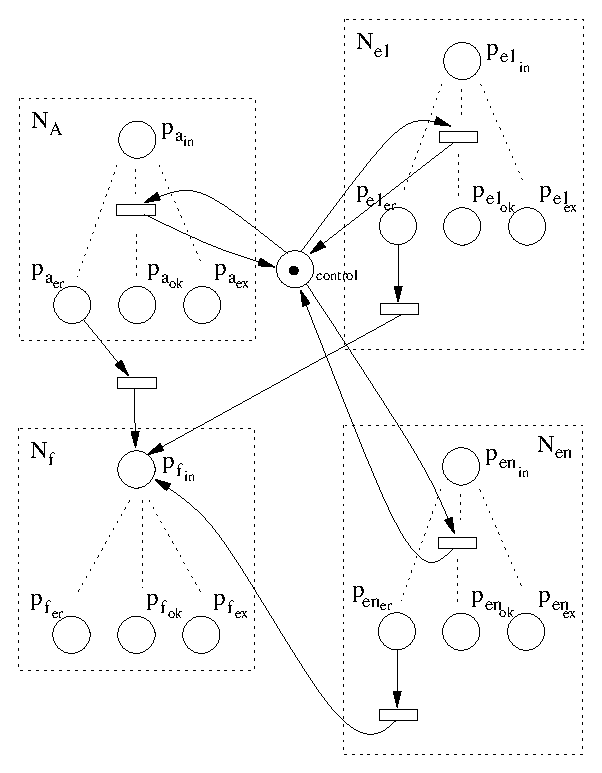
\includegraphics[scale=0.5]{Figures/orchestration.eps}
}}\end{center}
\vspace{-0.65cm}
\caption{Orchestration Translation}\label{orchestator}
\vspace{-0.5cm}
\end{figure}

%where \mbox{$e \in \nat$} is a natural value reserved to 
%represent that the variable has not yet been assigned.
 
%\item {\em Activities}\,:\, The translation for each one is shown in
%the following subsections.
%\end{itemize}


{\it Variables and resources}: There is one place for each variable, whose token value is the current variable value. As regards resources, there are two places associated to each resource, $p_{\it r_i}$, $p_{\it r_a}$. For
any resource {\it r}, ${\it p_{r_a}}$ becomes marked when the orchestrator executes the \emph{createResource} activity, whereas the second one, ${\it p_{r_i}}$, is marked as far as the orchestrator does not execute the \emph{createResource} activity. When the resource lifetime terminates, the resource is released, passing the token from ${\it p_{r_a}}$ to ${\it p_{r_i}}$. Observe that we can know in advance the number of resources in the system by reading the WS-BPEL/WSRF document.

%After presenting the places that conform our timed net, we are going to analyse thoroughly the activities that constitute the process logic. We will start with the basic activities.

% ======================================================================
%                            BASICAS 
%=======================================================================

\subsection{Basic activities}
\begin{itemize}
\item {\it Throw, Empty, Assign, Exit} and  {\it Wait} activities:\\
%
These are translated as indicated in \mbox{Fig.\ \ref{fig:basicas}},
by means of a single transition labelled
with the name of the corresponding activity linked with the corresponding terminating place. 
The time required  to execute 
{\it assign}, {\it empty}, {\it throw} and {\it exit} is negligible, so that the 
corresponding transitions have a null delay associated.
Notice that for the {\em assign} activity translation we use
a self loop between the transition and the
place associated with the variable ($p_{\it v}$)
in order to replace its previous value by the new one, being this new value obtained from an expression (exp) consisting of variables $p_{v1},\ldots,p_{vn}$ and integers. For the {\it wait}
activity, we have a time interval $[a,b]$ associated, so the delay is randomly selected
inside this interval.\\
Notice the use of a ``control'' place, to arrest all possible remaining activities in the system when either throw or exit are executed. Thus, the idea is that all transitions in the net must be connected with this place, as the different illustrations show.
\vspace{-1.3cm}
%\begin{figure}[!ht]
%\hspace*{1.0cm}
%\begin{center}
%\fbox{ \parbox[t]{12cm}{ \center
%\subfloat[Throw PTCPN]{\label{fig:throw}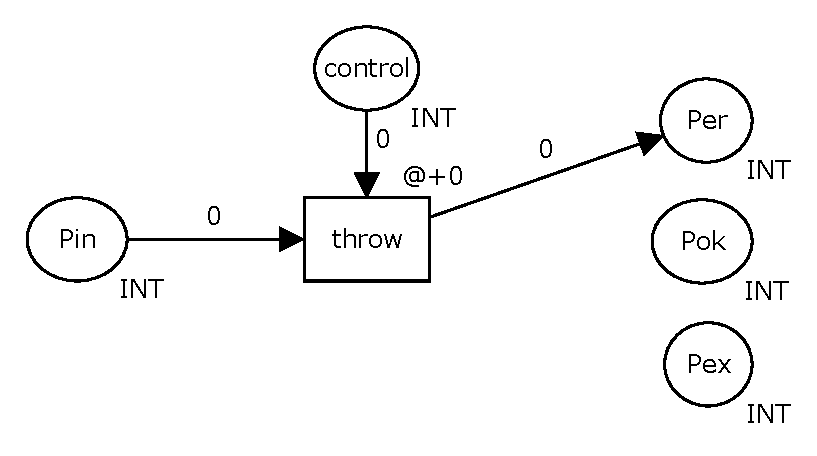
\includegraphics[scale=0.3]{Figures/throw.eps}}
%\subfloat[Exit PTCPN]{\label{fig:exit}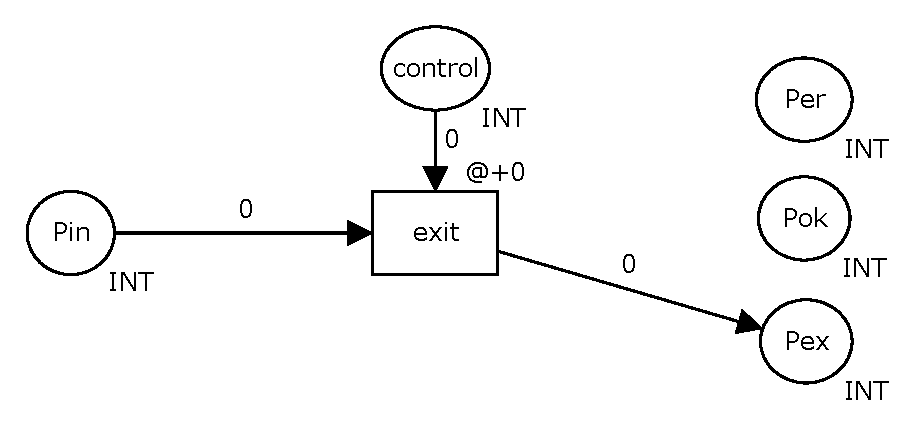
\includegraphics[scale=0.3]{Figures/exit.eps}}
%\subfloat[Empty PTCPN]{\label{fig:empty}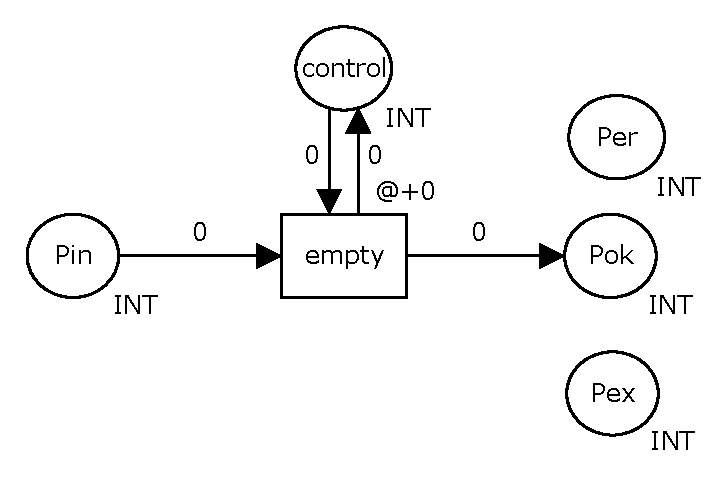
\includegraphics[scale=0.3]{Figures/empty.eps}}\\
%\subfloat[Wait PTCPN]{\label{fig:wait}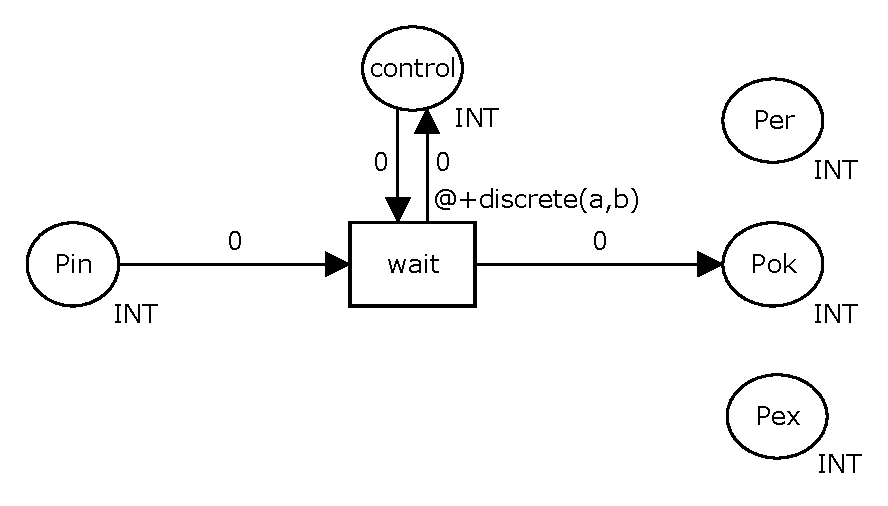
\includegraphics[scale=0.3]{Figures/wait.eps}}
%\ \ \ \ \subfloat[Assign PTCPN]{\label{fig:assign}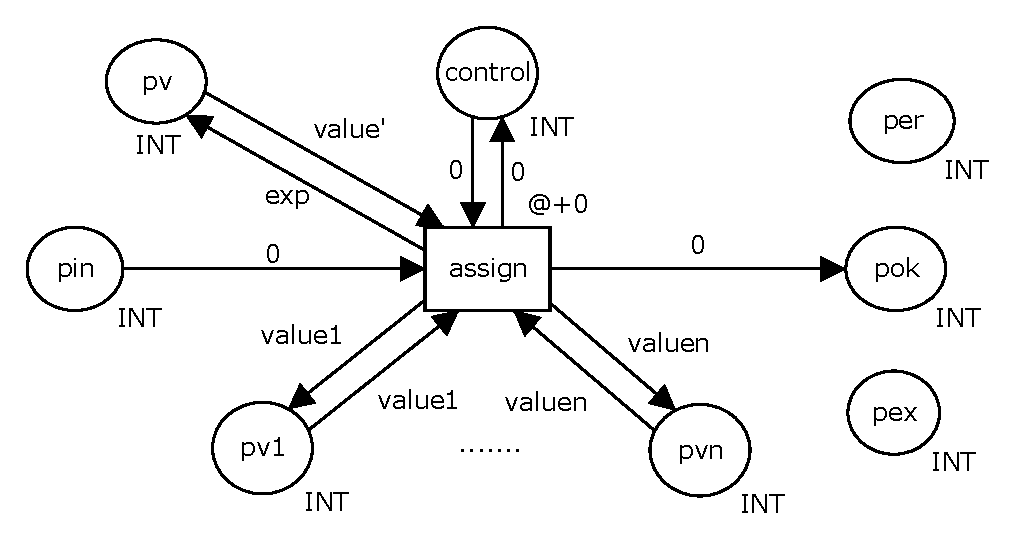
\includegraphics[scale=0.3]{Figures/assign.eps}}
%}}
%\end{center}
%\vspace{-0.6cm}
%\caption{\label{fig:basicas}Basic Activities
%Translation}
%\vspace{-0.5cm}
%\end{figure}
%\newpage

\item {\it Communication activities}:
The model we use is based on the invoke and receive operations, 
as well as the reply activity that uses a server to reply to a client. We have also added a barred version
of reply to synchronise with the response from the client. We have therefore introduced 
this last activity in our semantics to deal with the synchronous or asynchronous nature of invoke activity (one-way or request-response operation, respectively), so the $\overline{reply}$ activity is optional in the syntax depicted in Table \ref{BPELsyntax}. 
\vspace{-0.7cm}
%\begin{figure}[!ht]
%\vspace{-0.5cm}
%\hspace*{1.0cm}
%\begin{center}
%\fbox{ \parbox[t]{13cm}{ %\center 
%\hspace{-0.2cm}\subfloat[Invoke/Receive PTCPN]{\label{fig:comm1}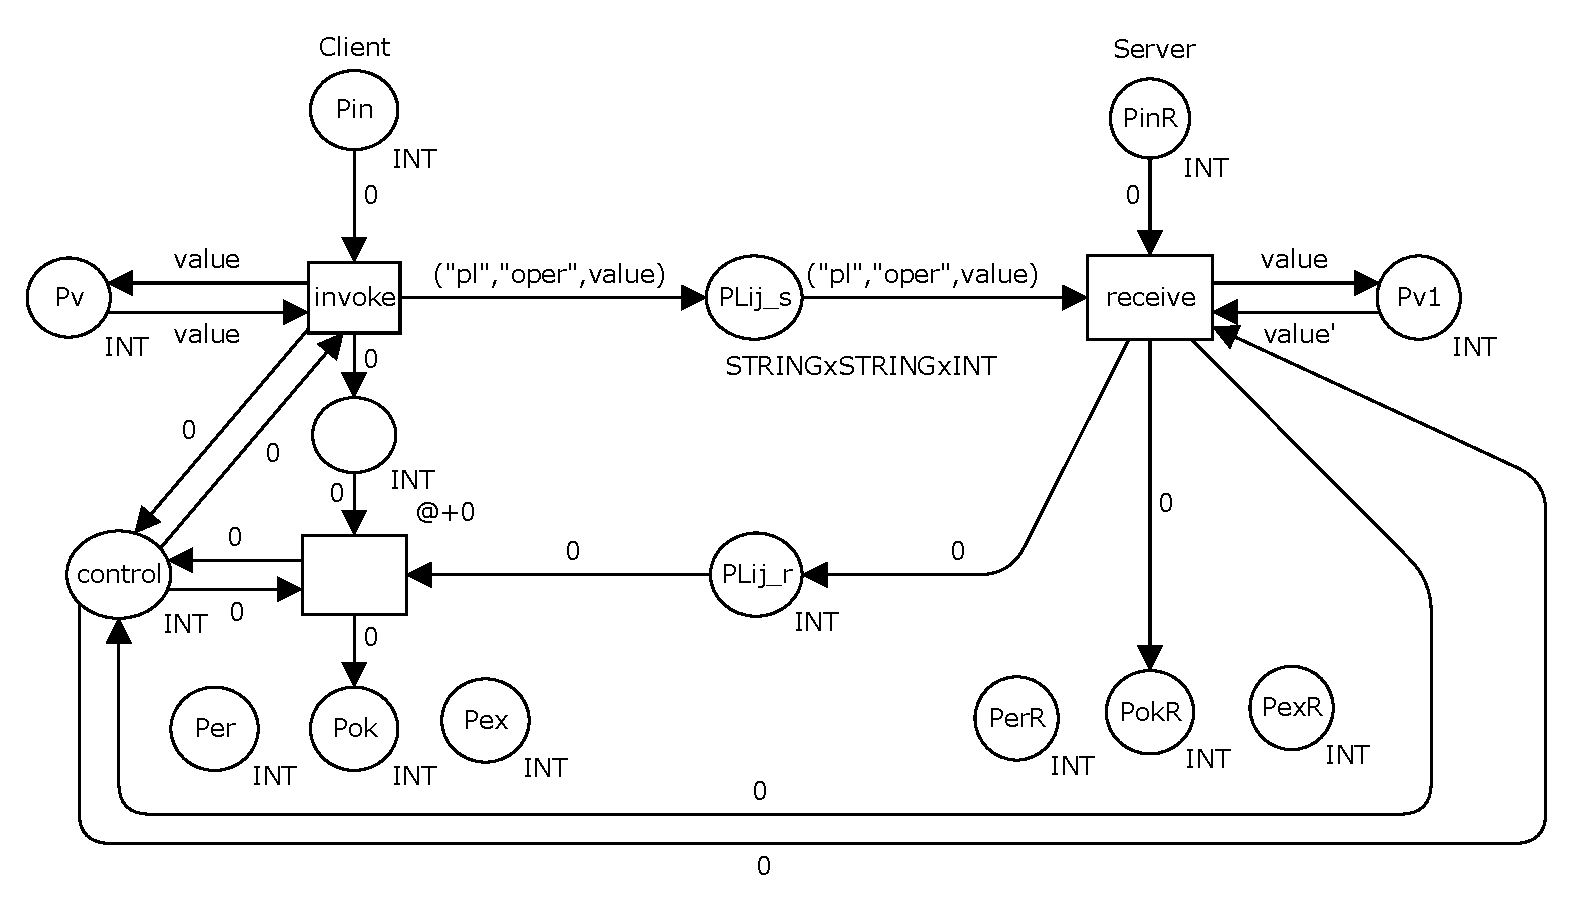
\includegraphics[scale=0.27]{Figures/communication.eps}}
%\subfloat[$\overline{Reply}$/Reply PTCPN]{\label{fig:comm2}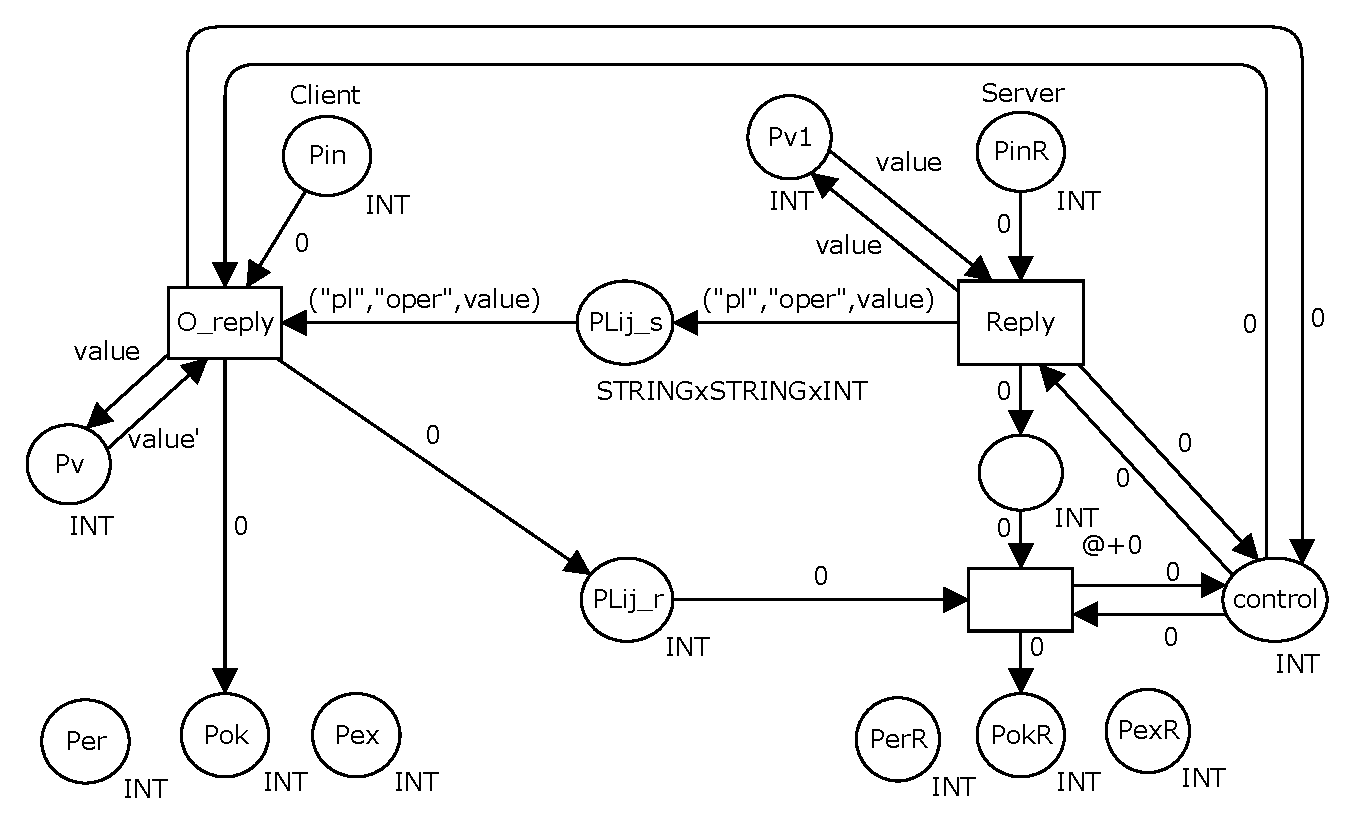
\includegraphics[scale=0.27]{Figures/communication_2.eps}}
%}}
%\end{center}
%\vspace{-0.62cm}
%\caption{\label{fig:comm}Invoke/Receive Activities
%Translation}% \vspace{1cm}
%\vspace{-0.5cm}
%\end{figure}

%In this case, we have added to our timed Petri net two specific places in order to manage the execution of invoke/receive and reply/$\overline{reply}$, $PLij\_s$ and $PLij\_r$. Thus, we only require two places to represent all the partnerlinks between two services since we will bind each one with its corresponding counterpart by using the colours of the tokens. Place $PLij\_s$ receives tokens with three parameters: $pl,op$ and $value$, whereas $PLij\_r$ is marked only when the activity has received the data, so this place is marked with the value 0. For the sake of simplicity, we exchange only the value of the variables, but this could be easily extended to any kind of data. We depict the Petri nets in Fig. \ref{fig:comm} that express the communication among partners. In Fig. \ref{fig:comm1}, the \emph{invoke} activity extracts the value to send from the variable place ${\it P_v}$ and mark the ``sending'' partnerlink with a token endowed with this information. Once this place is marked, the receive transition can be fired marking $PLij\_r$ to allow the invoke activity to continue, and storing directly the data exchanged in the corresponding variable place. The interpretation of Fig. \ref{fig:comm2} is analogous.  
Fig.~\ref{fig:comm} shows the translation for both the invoke/receive and the reply/$\overline{reply}$ pairs of activities. Part \ref{fig:comm1} of the figure corresponds to the invoke/receive translation, in which the net of the invoke activity is depicted on the left-hand-side part, whereas the receive activity is depicted on the right-hand-side part. There are two shared places, $PL_{ij{_s}}$ and $PL_{ij{_r}}$, which are used to implement the synchronisation between the invocation and reception of services. Both places are associated to the partnerlink used for this communication, denoted here by $(i,j)$, where $i$ and $j$ are the orchestrator identifiers performing those activities. Notice that the value of a single variable is transmitted, which is obtained from the corresponding variable place, $p_v$. In the same way, the receive activity stores this value in its own variable. The interpretation of Fig.~\ref{fig:comm2} is analogous.  
\end{itemize}
%
% ======================================================================
%                            ORDERING 
%=======================================================================
\subsection{Ordering structures}

%Structured activities prescribe the order in which a collection of activities is executed. They 
%describe how a business process is created; by composing the basic activities and the WSRF-compliant activities (presented previously)
%it performs into structures that express the control patterns, handling of 
%faults and external events, and coordination of message exchanges between process instances 
%involved in a business protocol.  
WS-BPEL defines structured activities for various control-flow patterns:
\begin{itemize} 
\item Sequential control between activities is provided by $<$sequence$>$, $<$if$>$, \linebreak $<$while$>$, 
$<$repeatUntil$>$, and the serial variant of $<$forEach$>$. 
\item Concurrency and synchronization between activities is provided by $<$flow$>$ and the 
parallel variant of $<$forEach$>$.  
\item Deferred choice controlled by external and internal events is provided by $<$pick$>$.  
\end{itemize}
The set of structured activities in WS-BPEL is not intended to be minimal \cite{BPEL4WS}, so there are cases where 
the semantics of one activity can be represented using another activity. Nevertheless, in order to reduce the complexity
of our translation, our approach omits many derived activities only dealing with the most important ones from the modelling viewpoint,
such as sequence, parallel and choice. For all these cases we provide the translation
by only considering two activities. However, the generalization
to a greater number of activities is straightforward in all
of them. 
\begin{itemize}

\item {\it Sequence}\,: A sequence of two activities $A_1;A_2$ (with PTCPNs $N_{A_1}$ and
      $N_{A_2}$, respectively)
      is translated in a simple
      way (Fig.\,\ref{seq}), by just collapsing in a 
      single place (this will be
      an internal place of the new PTCPN)
      the {\it output} place ${\it Pok}$ of $N_{A_1}$, and the
      {\it entry} place of $N_{A_2}$.  The {\it entry} place
      of the new PTCPN will
      be the {\it entry} place of $N_{A_1}$. The
      {\it output} place of the new PTCPN will
      be the {\it output} place of  $N_{A_2}$, and we also
      collapse the {\it exit}, {\it error} and {\it control}  places of both PTCPNs.

%\vspace{1cm}

\begin{figure}[!ht]
\vspace{-0.5cm}
\begin{center}
\fbox{\parbox[]{6cm}{\center
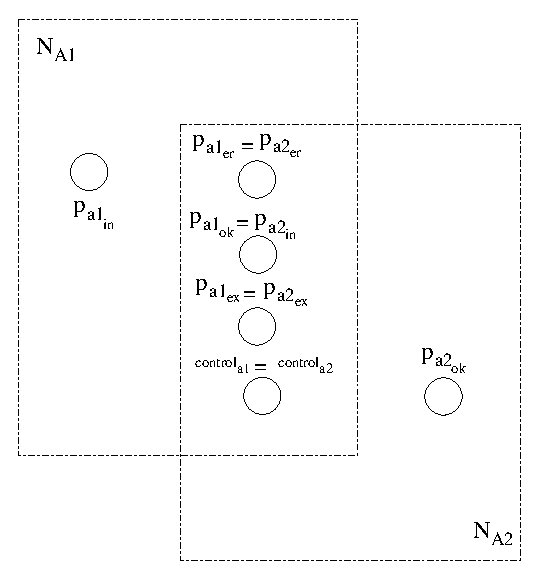
\includegraphics[scale=0.5]{Figures/sequence.eps}}}
\end{center}
\vspace{-0.65cm}
\caption{\label{seq} Sequence Translation}
\vspace{-0.6cm}
\end{figure}

\item {\it Parallel}\,: The translation for a parallel activity is depicted
in Fig.\,\ref{par}, which includes two new transitions $t1$ and
$t2$. The first to fork both parallel activities
and the second to join them when correctly terminated. 
Transition $t1$ thus puts one token on the initial places of both
PTCPNs, $N_{A_1}$ and $N_{A_2}$, in order to activate them,
and also puts one token on a new place, $p_c$, which is
used to stop the execution of one branch when the other has
failed or the exit activity is explicitly executed in one of them.
This place is therefore a precondition of every 
transition in both PTCPNs, and it is also a postcondition
of the non-failing transitions. However, in the event
of a failure or an exit activity, the corresponding {\em throw} or {\em exit}  transition
will not put the token back on $p_c$, thus
arresting the other parallel activity.

Notice also that the {\em error} places of ${N}_{A_{1}}$ and $N_{A_{2}}$
have been joined in a single error place ($p_{\it er}$),
which becomes marked with one token on
the firing of one {\em throw} transition. 
In this case, the other activity cannot execute any
more actions ($p_c$ is empty), so some dead tokens would
remain permanently on some places in the PTCPN.
However, these tokens cannot cause
any damage, since the control flow has been
transferred either to the fault handling activity of the PTCPN, 
once the place $p_{er}$ has become marked, or the whole system has terminated once 
the place $p_{ex}$ is marked. %A similar reasoning is done with the {\em exit} places.
%It is a need to remark we do not treat 
%some BPEL flow construction attributes such as join conditions,
%dead path elimination, etc., since is out of the scope of this paper.
\begin{figure}[!ht]
\vspace{-0.75cm}
\begin{center}
\fbox{\parbox[t]{12cm}
{\begin{center}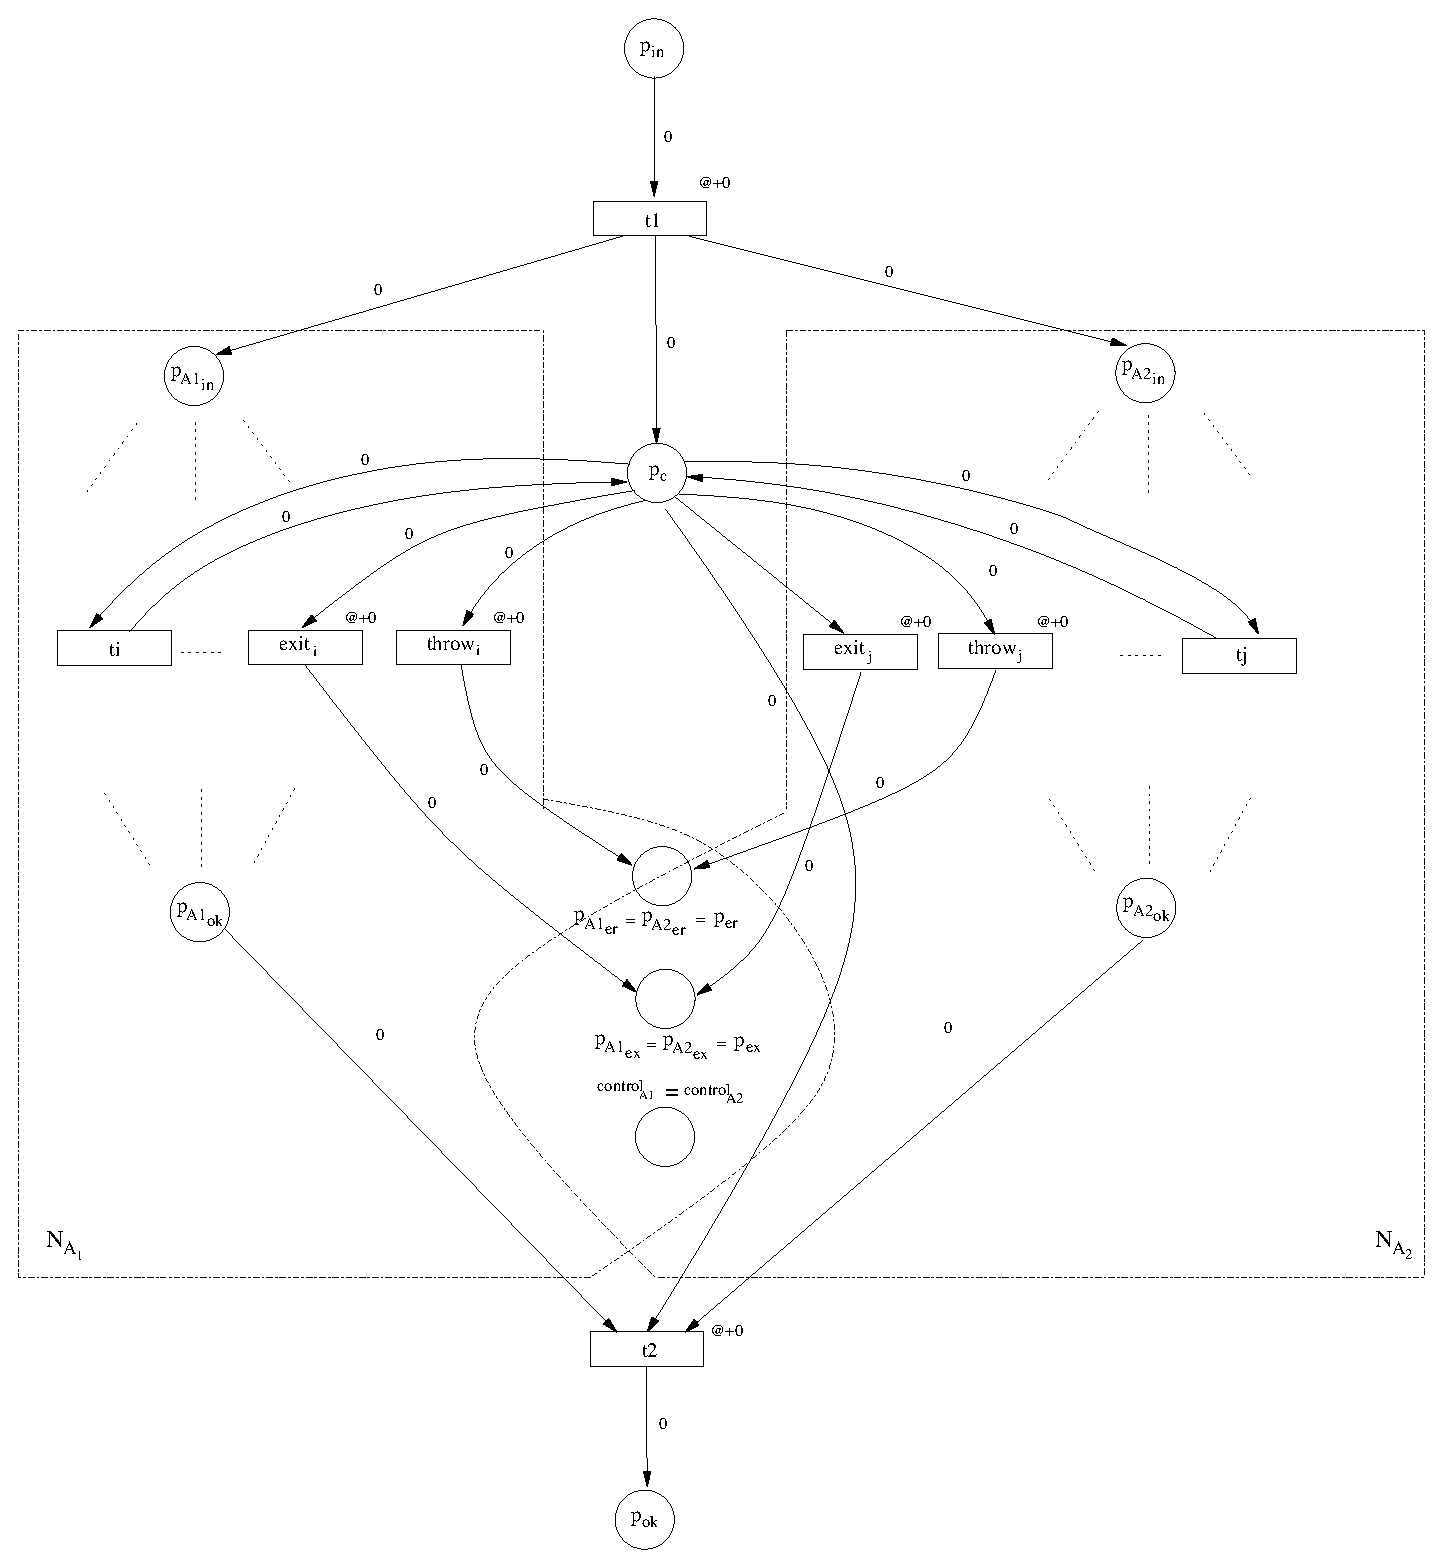
\includegraphics[height=10cm,width=12cm]
{Figures/paralelo.eps}\end{center}}}
\end{center}
\vspace{-0.7cm}
\caption{\label{par} Parallel Activity Translation.}
\vspace{-0.5cm}
\end{figure}

\item {\it Pick} $(\{(pl_i,op_i,v_i,A_i)\}_{i=1}^n,A,timeout)$: The $<$pick$>$ activity waits for the occurrence of exactly one event from a set of events, also establishing a
time-out for this selection. The translation is depicted in Fig.~\ref{pick} where a timer is implemented on the place {\it p\_a} in order to enforce the firing of transition {\it ta} when the timeout has elapsed, thus activating {\it N$_{A}$}. Notice also the use of both timed and untimed places in this figure, respectively called {\it INT} and {\it UINT}.  %The $<$pick$>$ activity completes when the selected activity finishes.
%, then 
%executes the activity associated with that event. After an event has been selected, the other events 
%are no longer accepted by that $<$pick$>$. The $<$pick$>$ activity is comprised of a set of branches, each containing an event-activity pair.  
 %The activities contained in this construction can come in two forms: 

%\begin{itemize}
%\item The $<$onMessage$>$ is similar to a $<$receive$>$ activity, in that it waits for the receipt of an 
%inbound message. 
%\item The $<$onAlarm$>$ corresponds to a timer-based alarm. If the specified duration value 
%is zero or negative, or a specified deadline has already been reached or 
%passed, then the $<$onAlarm$>$ event activity is executed immediately. 
%\end{itemize} 
% must act in a similar fashion, but adding a feature
%which permits the selection among some activities. This selection is easy to model with Petri nets since collapsing the input places of the possible branches
%it is impossible to execute more than one at the same {\em pick}. In our model, the place {\em PinA1..An} represents this behaviour. Finally, in the BPEL specification, 
%is encouraged the use of time-outs with {\em pick} activity, so we have included a timed transition with its corresponding timed guard in order to manage the execution of 
%an ``alarm activity'' only in the event the time-out expires. The meaning of the other places and transitions is the same as in the receive activity.  

\item {\it While} (cond,A): The machinery needed to model this construction is fairly straightforward since we only must check if the repetition condition holds or not in order to execute the contained activity or skip it. Fig.~\ref{while} shows this translation.
\end{itemize}
%The $<$while$>$ activity provides for repeated execution of a contained activity. The contained 
%activity is executed as long as the boolean condition evaluates to true at the beginning of 
%each iteration. The meaning of the places and transitions of the net represented in Fig. \ref{while} is fairly straightforward, so, due to space limitations, we are going to omit any explanation of its elements. 
%The meaning of the places and transitions are fairly straightforward, so, due to space limitations, we are going to omit any explanation of the elements contained in this net 
%\newpage

\begin{figure}[!ht]
%\vspace{-0.5cm}
\begin{center}
\fbox{\parbox[c]{12cm}{\begin{center}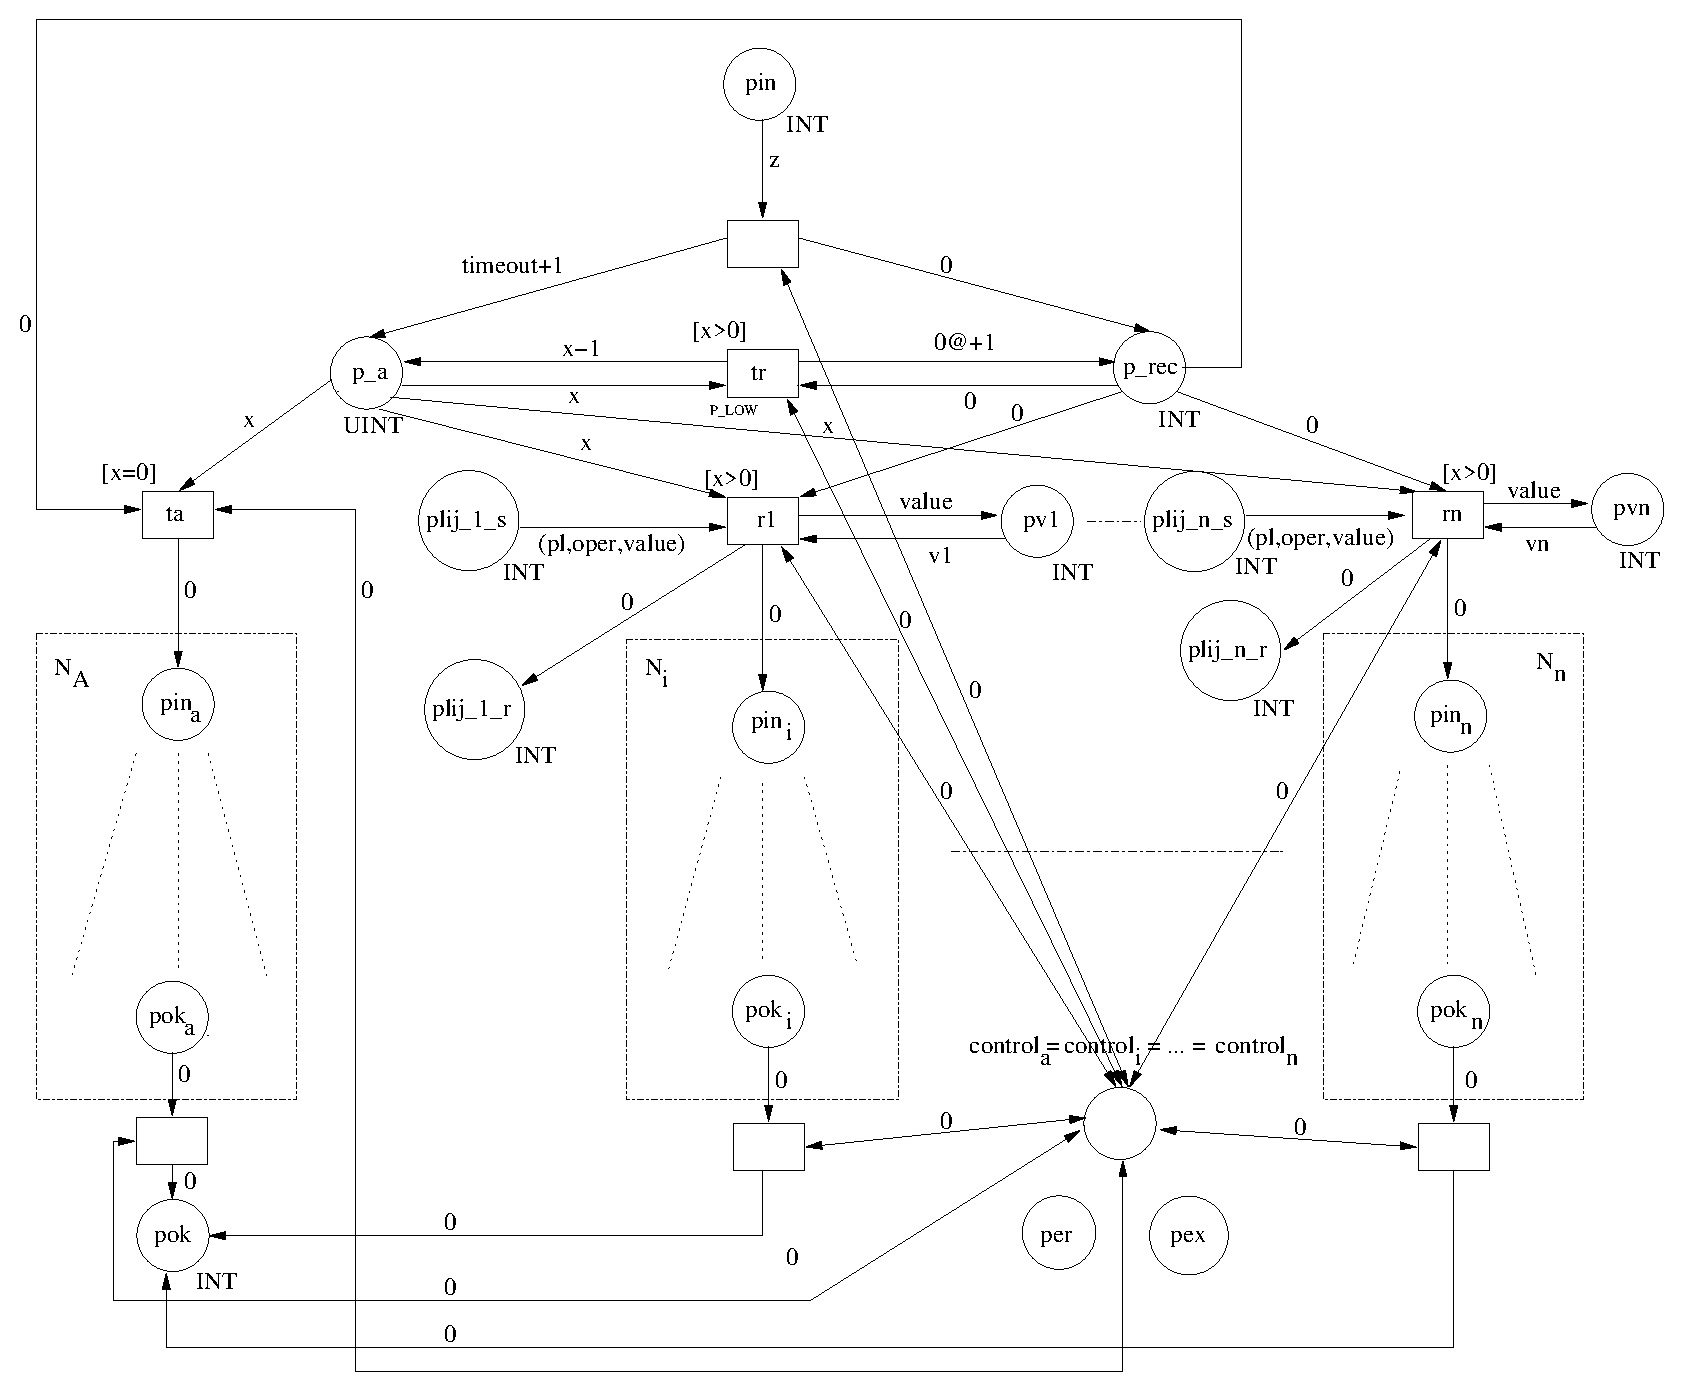
\includegraphics[scale=0.4]
{Figures/pick.eps}\end{center}}}
\end{center}
\vspace{-0.6cm}
\caption{\label{pick} Pick Activity Translation.}
%\vspace{-0.4cm}
\end{figure}

%\vspace{-1.3cm}

\begin{figure}[!ht]
%\vspace{-0.7cm}
\begin{center}
\fbox{\parbox[t]{11cm}{\begin{center}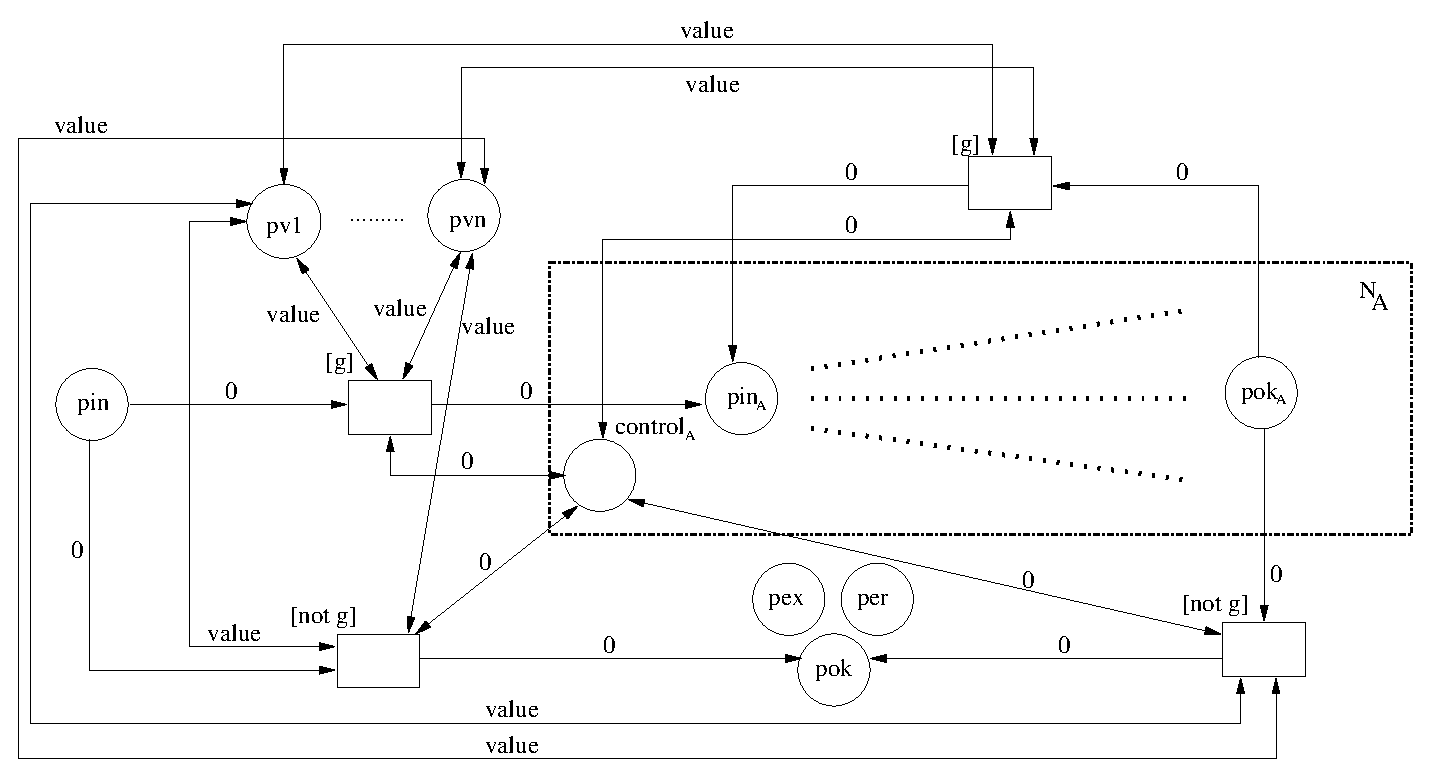
\includegraphics[scale=0.4]
{Figures/while.eps}\end{center}}}
\end{center}
\vspace{-0.65cm}
\caption{\label{while} While Activity Translation.}
\vspace{-0.7cm}
\end{figure}
\vspace{-0.5cm}
% ======================================================================
%                            WSRF 
%=======================================================================
\subsection{WSRF-compliant}
%In this section, we state the WSRF activities we have integrated with the BPEL activities in order to create a framework for modelling stateful workflows. It is worth noting that in recent years have appeared a new redefinition of workflow nets which deals with resources called Resource-Constrained Workflow Nets \ref{}. As commented in the Related Work section, this approach extends the well-known formalism, Workflow nets, with finite resources such as money, memory and so on, but the authors do not provide the machinery
%to create and destroy such resources, so this extension of Workflow nets matches with the idea of WSRF standard, i.e., the creation and destruction of resources is out of the scope of the specification. Nevertheless, our approach was devised to manage the whole lifetime of the resource from its creation until its destruction.


%To date, we have presented the activities corresponding to the ``BPEL'' activities part of our model. Next, we will state the counterpart of our approach, i.e., the activities, which permit the creation and modification of the resources as well as the management of the subscriptions to them following the indications of the standard WSRF. Notice that a novelty in our model is the creation of resources since WSRF does not specify how this creation is done.
%\begin{figure}[!ht]
%\vspace{-0.5cm}
%\begin{center}
%\fbox{\parbox[t]{12cm}{\begin{center}\includegraphics[scale=0.35]
%{Images/createResource.eps}\end{center}}}
%\end{center}
%\vspace{-0.7cm}
%\caption{\label{createresource} CreateResource Activity Translation.}
%\vspace{-1.5cm}
%\end{figure}

%To begin with, we depict the creation of resources in Fig. \ref{createresource}. In order to guarantee our PTCPNs are 1-safe, we opted as commented above to model each resource with two dedicated places,  $p_{\it r_i}$, and $p_{\it r_a}$, which represent the possible state of the resources, instantiated or not instantiated, respectively. Thus, when an orchestrator wants to create a resource, the firing of the transition {\it createResource} moves the token from the ``inactive'' ($p_{\it r_i}$) to the ``active'' place ($p_{\it r_a}$) making available this resource to the subscribers. Once the place $p_{\it r_a}$ is marked and an orchestrator executes the activity {\em subscribe}, our translation can automatically build the subscriptions nets. Here, a subscription net is formed by a transition, whose guard is the subscription condition, and the subnet which corresponds to the translation of the activity that the subscriber wants to be executed just in case the subscription condition ${\it gc_i}$ holds. Notice that WSRF allows the creation of multiple subscriptions to the same resources by the same orchestrator, so we will allow this restriction. Despite the {\em subscribe} construction will be presented later, just comment here we have endowed each resource with a list that represents its subscribers with their {\em id} and an integer, $0$ or $1$, to denote whether the orchestrator with identifier {\em id} is subscribed or not. Finally, in the leftmost part of Fig. \ref{createresource}, we depict the net that will be fired in the event of the resource lifetime expires. In this situation, we return the token from the active place to the inactive place and immediately execute the activity {\em $Activity_timeisup$}, which will be passed as an argument of the {\em createResource} activity. This argument is not included in the WSRF specification, but we have incorporated it to show the benefits of the integration of both standards.       

%Now, we describe the PTCPNs who corresponds to the manipulation of resource value and lifetime as well the subscription to a specific resource. On the left side of Fig. \ref{fig:getproperty},
%the PTCPN for the activity {\em getProperty} is depicted. Here, the resource {\em value} obtained from $p_{\it r_a}$ is stored in the place of the corresponding variable. The reasoning done in the construction of the PTCPNs for the activities {\em setProperty} and {\em setTimeout} in Fig. \ref{fig:setproperty} is quite similar, but updating the resource value or its lifetime, respectively. Important to note that if an orchestrator is trying to access to a resource not instantiated, the fault place  $p_{\it er}$ will be marked starting the execution of the fault activity. 
%\begin{figure}[!ht]
%\vspace{-0.5cm}
%\hspace*{1.0cm}
%\begin{center}
%\fbox{ \parbox[t]{12cm}{ \center
%  \subfloat[GetProperty and Subscribe Activities]{\label{fig:getproperty}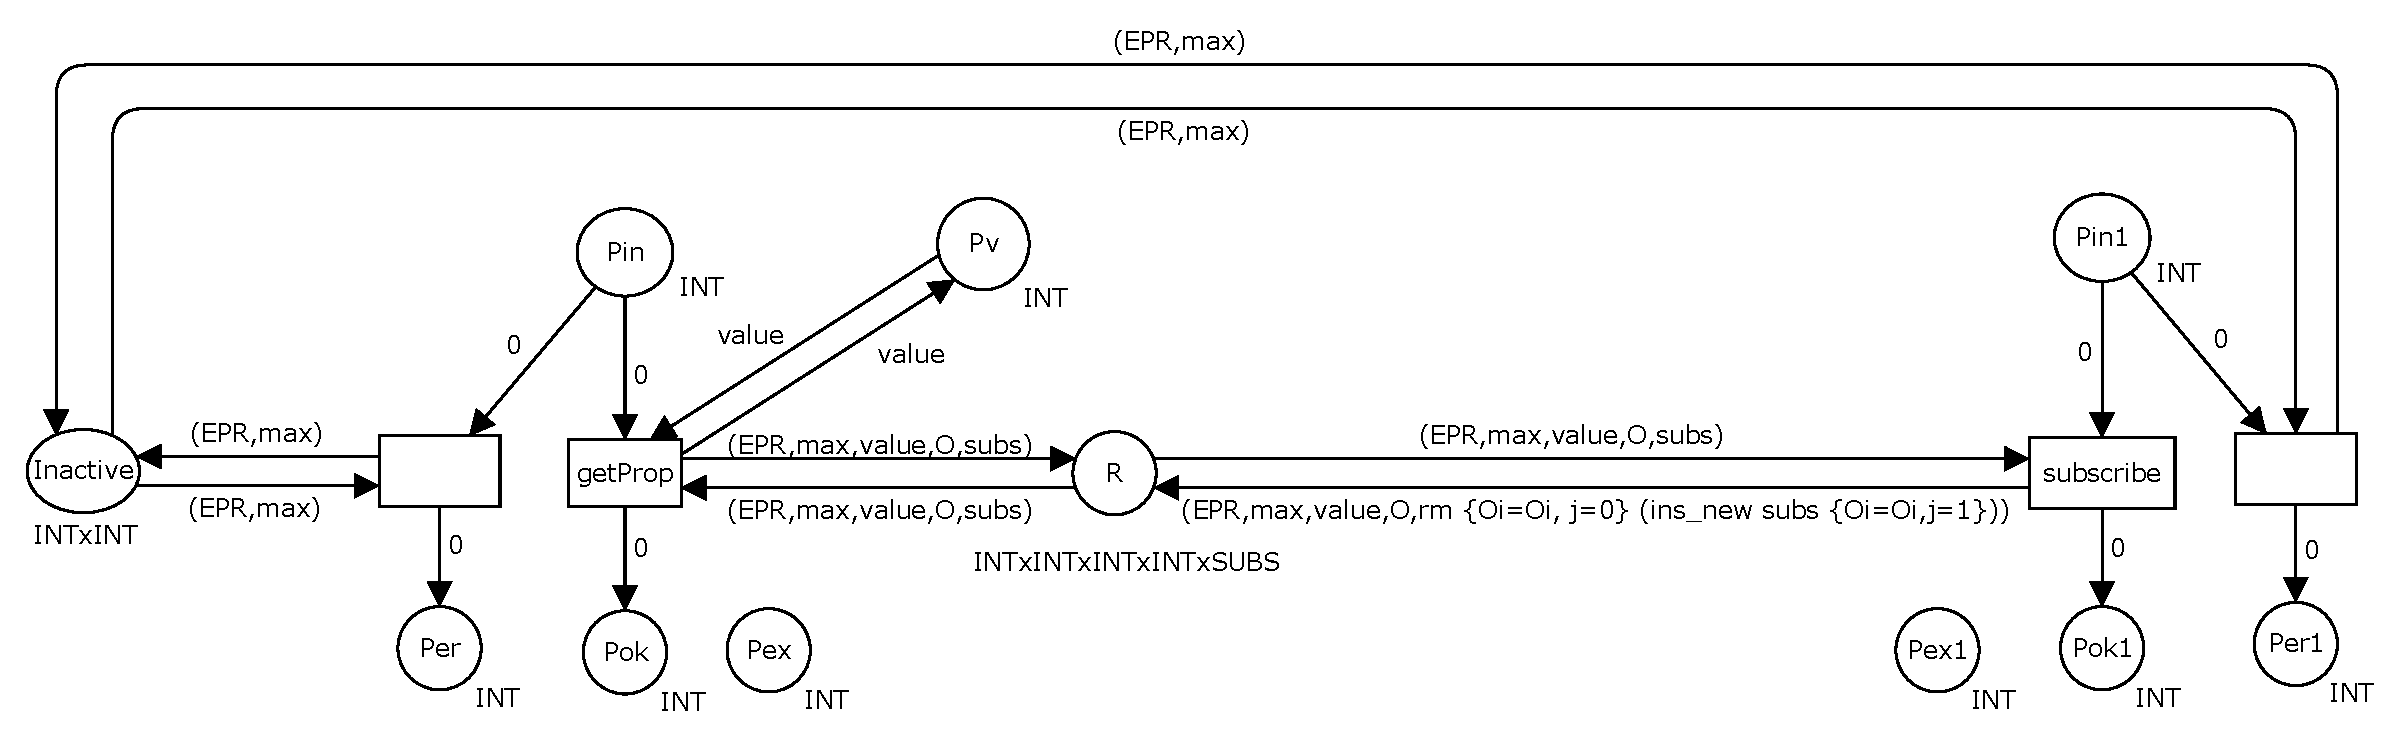
\includegraphics[scale=0.3]{Images/getProp+subscribe.eps}}\\
 % \subfloat[SetProperty and SetTimeout Activities]{\label{fig:setproperty}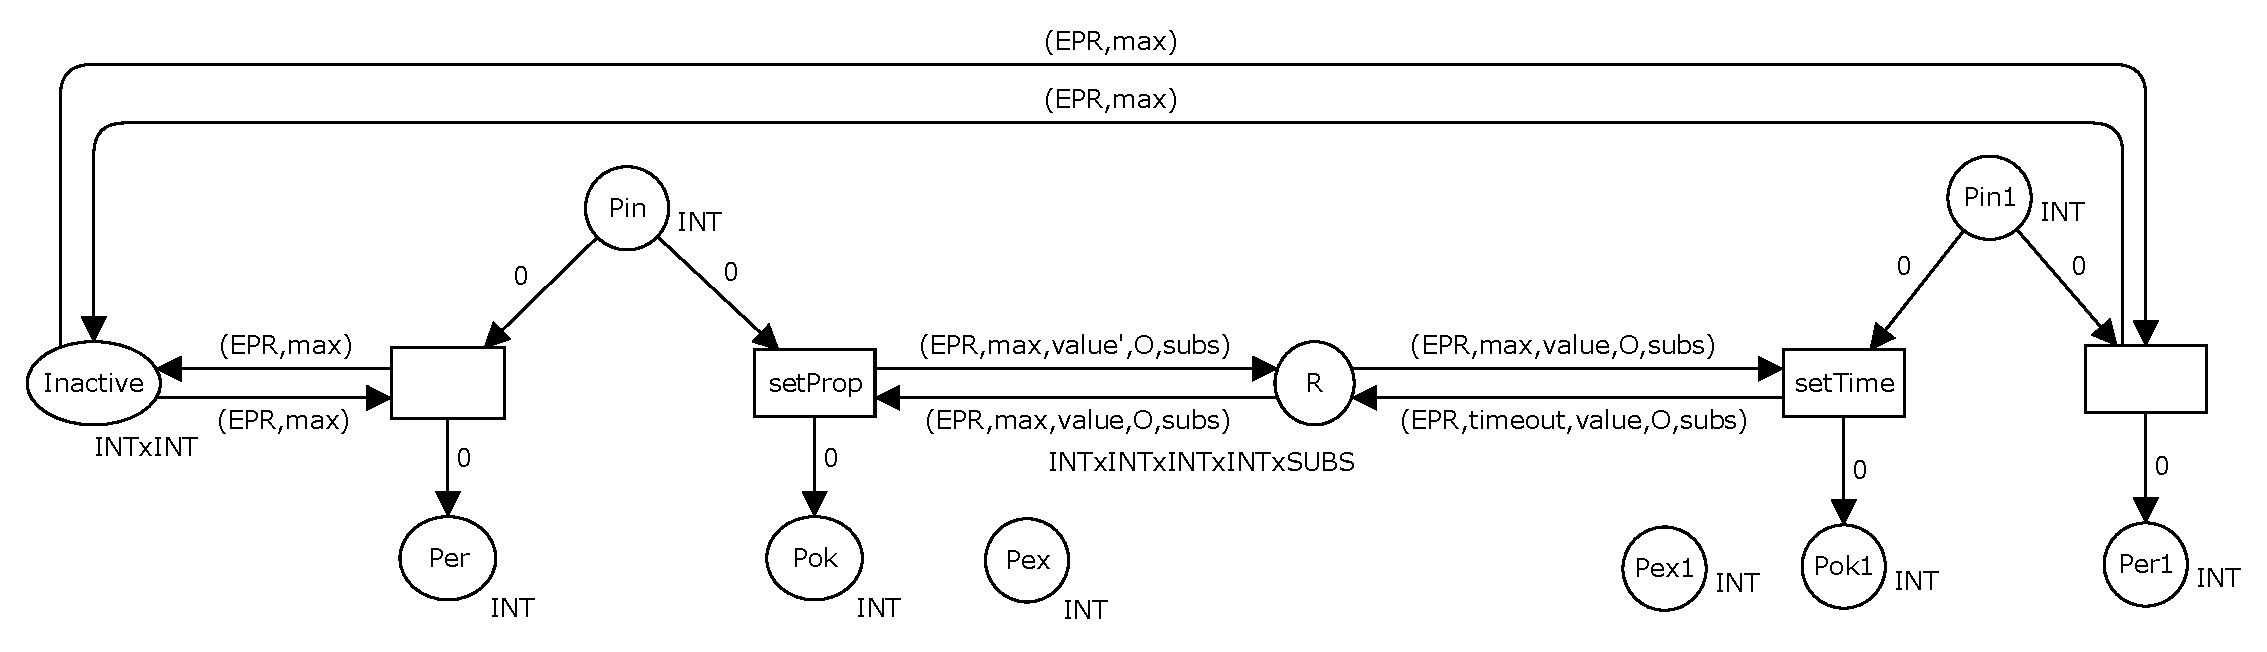
\includegraphics[scale=0.32]{Images/setProp+setTime.eps}}
 % }}
%\end{center}
%\vspace{-0.6cm}
%\caption{\label{fig_wsrf}WSRF Activities
%Translation}
%\vspace{-0.5cm}
%\end{figure}

%Finally, on the right side of Fig. \ref{fig:getproperty}, we show the PTCPN for the {\em subscribe} activity. Above, we have commented we have used a list to represent the subscribers of a resource. Since we have used CPNtools to build our nets, this ``registration stamp'' is modeled by using the record colour set provided by this tool. This record contains the identifier of the subscriber, {\em ID}, and integer variable {\em j}, whose value will be $0$ when the orchestrator is not subscribed and $1$ in the opposite case. This value will be checked in the guard of the first transition of the subscription net within the condition specified here in order to check if the orchestrator is subscribed and the condition holds. As in the previous cases, we run the fault activity if one orchestrator is trying to subscribe to non-instantiated resource.   

%\begin{figure}[!ht]
%\begin{center}
%\fbox{\parbox[t]{12cm}{\begin{center}\includegraphics[scale=0.35]
%{Images/setProp.eps}\end{center}}}
%\end{center}
%\vspace{-0.7cm}
%\caption{\label{setp} GetProperty Activity Translation.}
%\end{figure}

%\begin{figure}[!ht]
%\begin{center}
%\fbox{\parbox[t]{12cm}{\begin{center}\includegraphics[scale=0.35]
%{Images/getProp.eps}\end{center}}}
%\end{center}
%\vspace{-0.7cm}
%\caption{\label{setp} SetProperty Activity Translation.}
%\end{figure}

%\begin{figure}[!ht]
%\begin{center}
%\fbox{\parbox[t]{12cm}{\begin{center}\includegraphics[scale=0.35]
%{Images/setTime.eps}\end{center}}}
%\end{center}
%\vspace{-0.7cm}
%\caption{\label{settim} SetTimeout Activity Translation.}
%\end{figure}

%=============================Valentín================================
Let us now see the WSRF activities, and their corresponding translations.

\begin{itemize}
\item {\it CreateResource (EPR,val,timeout,A)}:
{\em EPR} is the resource identifier, for which we have two complementary places in Fig.~\ref{createresource}, ${\it p_{r_i}}$ and ${\it p_{r_a}}$, where the sub-index represents the state of the resource: $i$ when it is inactive and $a$ when it is active. The initial value is $val$, and $A$ is the activity that must be executed when the time-out indicated as third parameter has elapsed.

We can see in Fig.~\ref{createresource} how the transition $createResource$ removes the token from the {\em inactive} place, and puts a new token on the active place, whose colour contains the following information: resource identifier (EPR), its lifetime (max), and its value (val). %the owner (O) and the list of subscribers (initially, empty).
\begin{figure}[!ht]
\vspace{-0.7cm}
\begin{center}
\fbox{\parbox[t]{12cm}{\begin{center}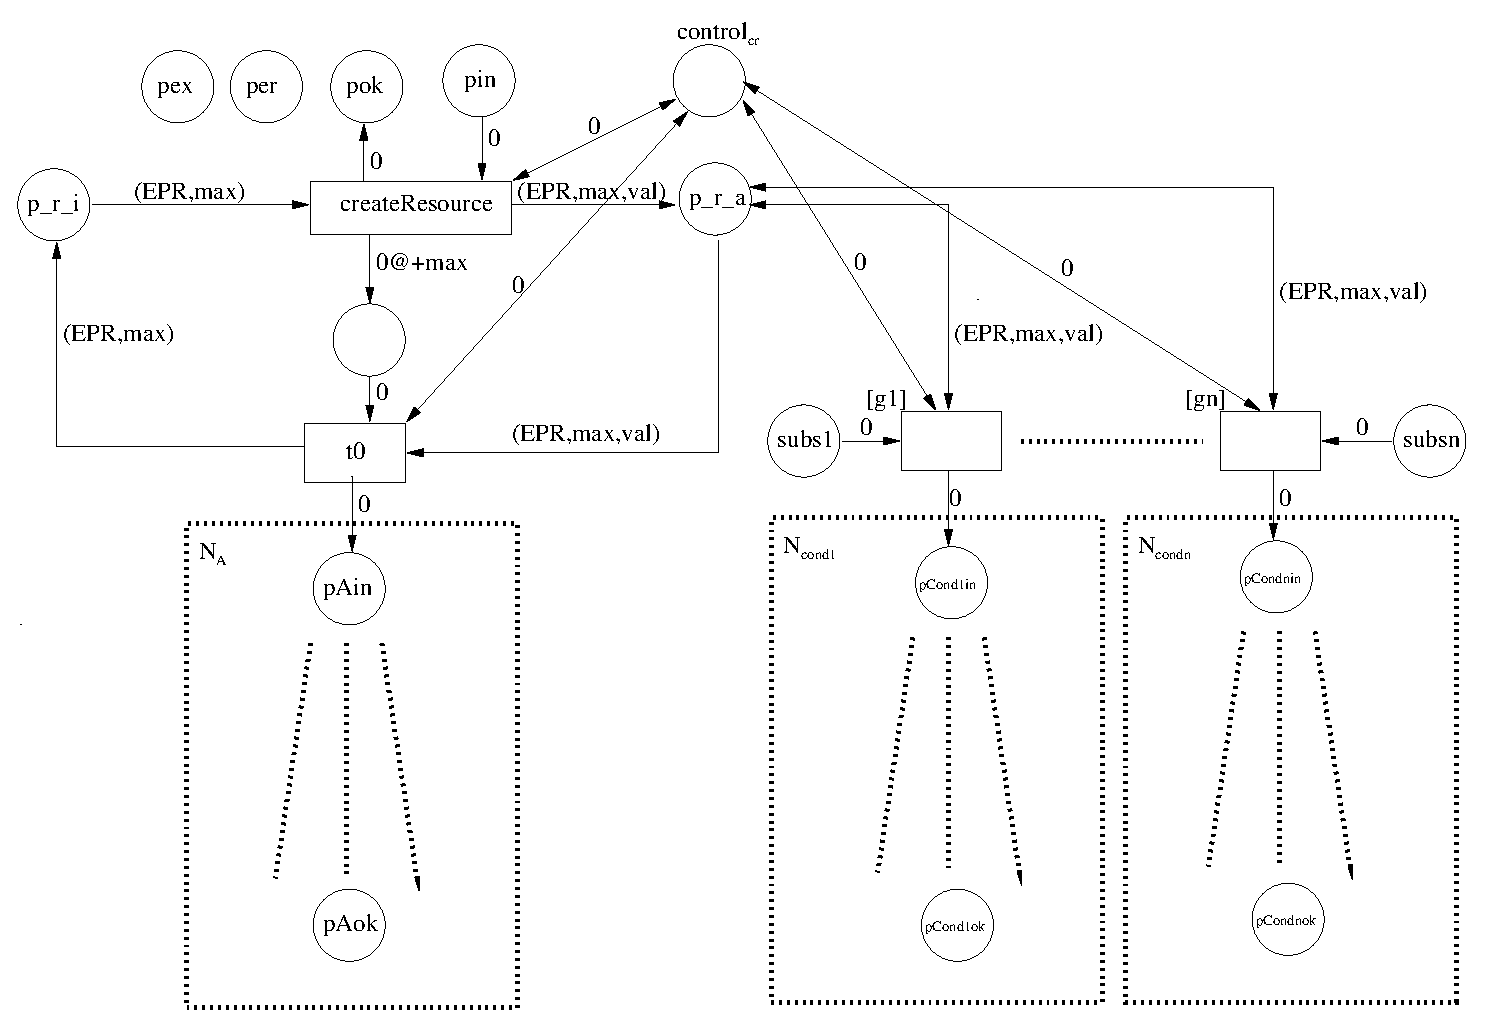
\includegraphics[scale=0.35]
{Figures/createResource.eps}\end{center}}}
\end{center}
\vspace{-0.7cm}
\caption{\label{createresource} CreateResource Activity Translation.}
\vspace{-0.5cm}
\end{figure}
Transition ${\it t}$0 is executed when the lifetime of the resource has expired, thus removing the token from the {\em active} place, marking again the {\em inactive} place, and activating $N_A$. We can also see that the {\em active} place is linked with a number of transitions, which correspond to the subscribers (we know in advance these possible subscribers from the WS-BPEL/WSRF document). These transitions can only become enabled if the corresponding places $subs_{i}$ are marked by performing the corresponding  activity {\em subscribe}. The PTCPNs ${\it Ncond_i}$ are the nets for the activities passed as parameter in the invocation of a subscribe activity.   
\item Subscribe (EPR,cond$'$,A):
In this case, an orchestrator subscribes to the resource $EPR$, with the associated condition $cond'$, upon which the activity $A$ must be performed. Fig.~\ref{subscribe} shows this translation, where we can observe that the associated place $subs_{i}$ is marked in order to allow the execution of the PTCPN for the activity $A$ if the condition $g_{i}$ holds. On the contrary, if the resource is not active, we will throw the fault handling activity.
%\begin{figure}[!ht]
%\vspace{-0.5cm}
%\hspace*{1.0cm}
%\begin{center}
%\fbox{ \parbox[t]{12cm}{ \center
%  \subfloat[GetProperty and Subscribe Activities]{\label{fig:getproperty}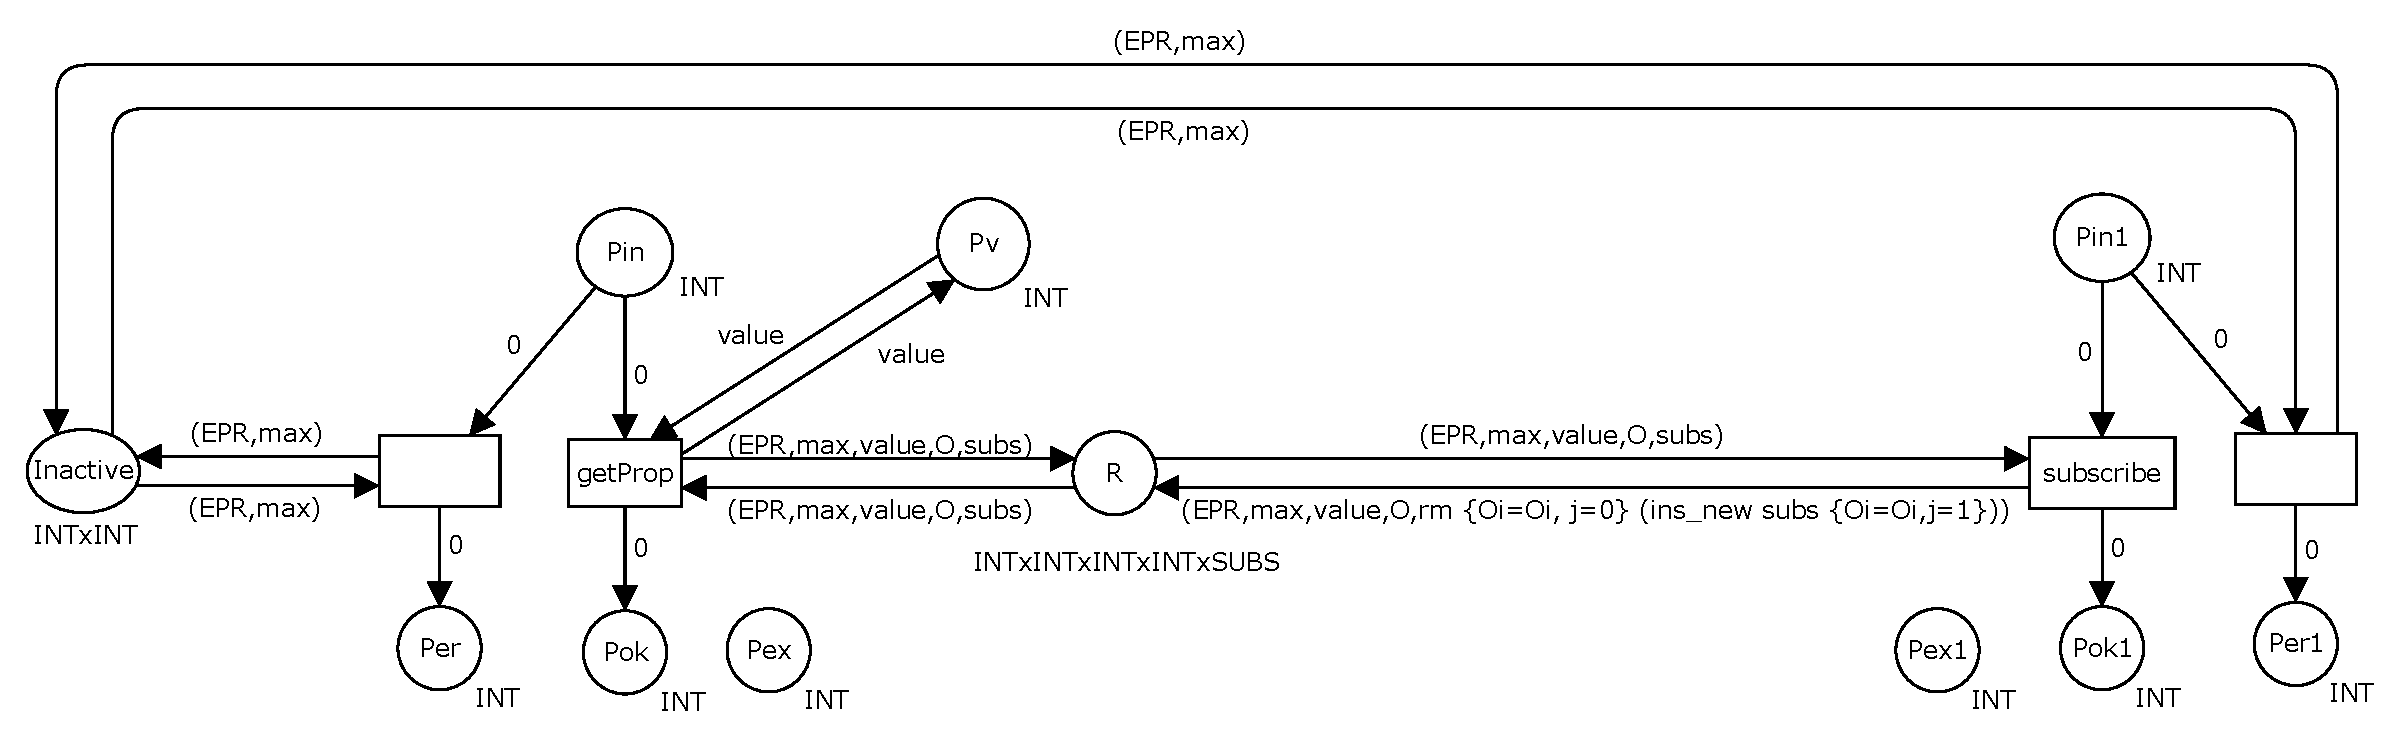
\includegraphics[scale=0.3]{Images/getProp+subscribe.eps}}\\
 % \subfloat[SetProperty and SetTimeout Activities]{\label{fig:setproperty}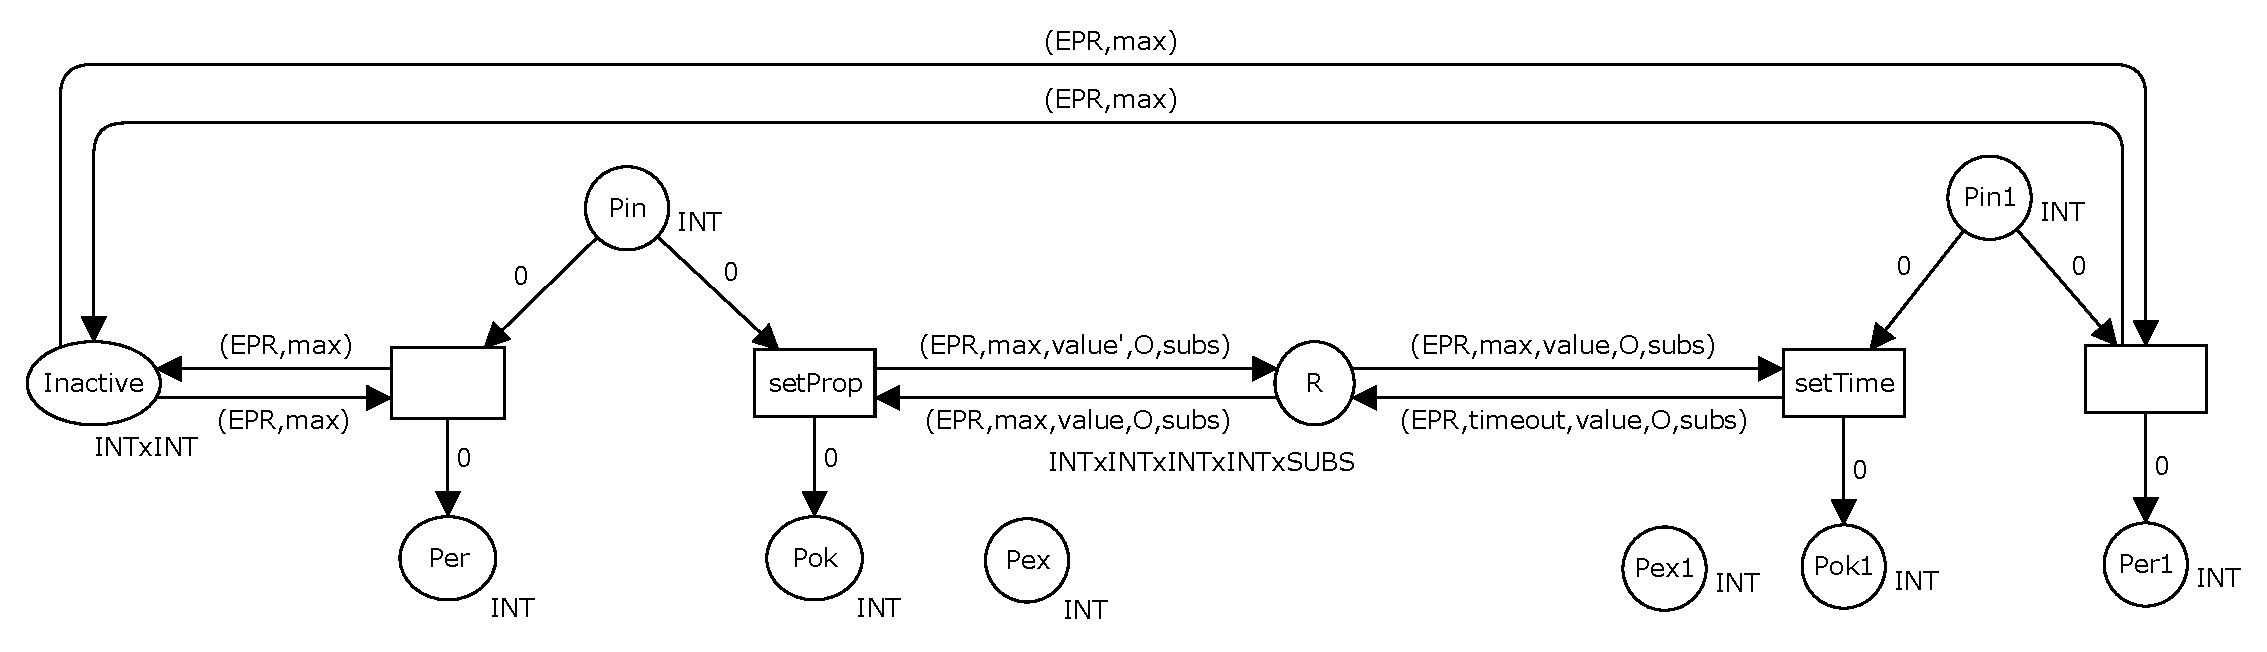
\includegraphics[scale=0.32]{Images/setProp+setTime.eps}}
 % }}
%\end{center}
%\vspace{-0.6cm}
%\caption{\label{fig_wsrf}WSRF Activities
%Translation}
%\vspace{-0.5cm}
%\end{figure}
\begin{figure}[!ht]
\vspace{1cm}
\begin{center}
\fbox{\parbox[t]{10cm}{\begin{center}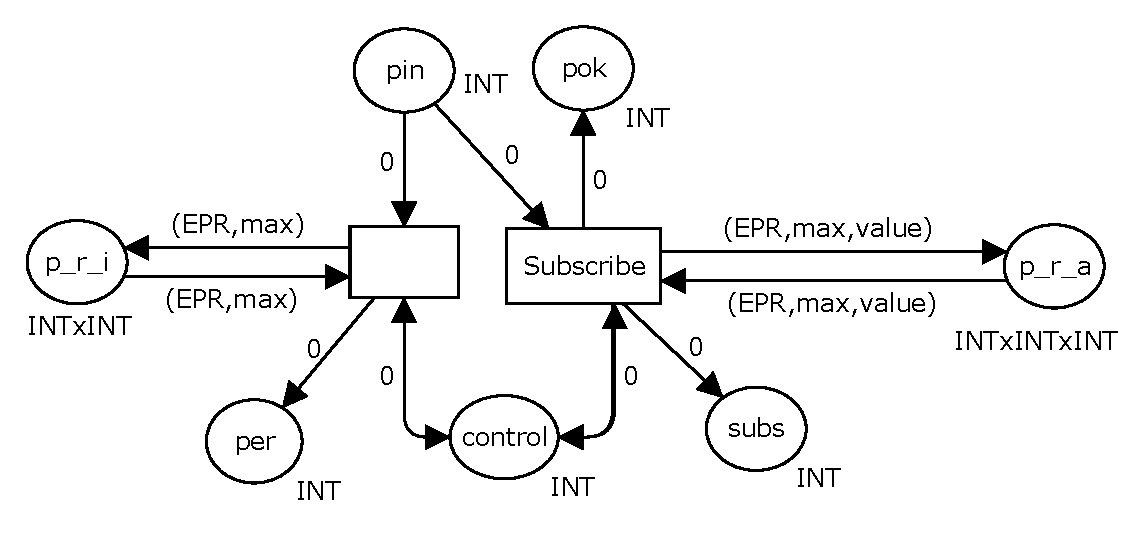
\includegraphics[scale=0.35]
{Figures/subscribe.eps}\end{center}}}
\end{center}
\vspace{-0.7cm}
\caption{\label{subscribe} Subscribe Activity Translation.}
\vspace{-0.5cm}
\end{figure}
\newpage
\item GetProp (EPR,v) and SetProp (EPR,expr):
These are easily translated, as shown in Figs.~\ref{getp} and \ref{setp}, where the resource value is obtained and assigned to variable $v$ (GetProp), or a new value is assigned to the resource (SetProp).
\vspace{-0.8cm}
\begin{figure}[!ht]
\begin{center}
\fbox{\parbox[t]{8.5cm}{\begin{center}\includegraphics[scale=0.35]
{Figures/getProp.eps}\end{center}}}
\end{center}
\vspace{-0.7cm}
\caption{\label{getp} GetProperty Activity Translation.}
\vspace{-0.7cm}
\end{figure}
%\begin{figure}[!ht]
%\vspace{-0.5cm}
%\hspace*{1.0cm}
%\begin{center}
%\fbox{ \parbox[t]{11cm}{ %\center 
%\hspace{-0.2cm}\subfloat[GetProperty Activity %Translation.]{\label{fig:get}\includegraphics[scale=0.4]{Images/getProp.eps}}\\
%\subfloat[SetProperty Activity %Translation]{\label{fig:set}\includegraphics[scale=0.4]{Images/setProp.eps}}\\
%\subfloat[SetTimeout Activity %Translation]{\label{fig:settime}\includegraphics[scale=0.4]{Images/setTime.eps}}
%}}
%\end{center}
%\vspace{-0.62cm}
%\caption{\label{fig:sg}GetProperty and SetProperty Activities
%Translation}% \vspace{1cm}
\vspace{-0.1cm}
%\end{figure}
%
%\newpage
\begin{figure}[!ht]
\begin{center}
\fbox{\parbox[t]{10cm}{\begin{center}\includegraphics[scale=0.35]
{Figures/setProp.eps}\end{center}}}
\end{center}
\vspace{-0.7cm}
\caption{\label{setp} SetProperty Activity Translation.}
\vspace{0.5cm}
\end{figure}

\item SetTimeout (EPR,timeout):
This activity is analogous to {\em SetProp} activity. In this case, the resource lifetime is updated with a new value. Fig.~\ref{setp} shows this translation. 
\begin{figure}[!ht]
\begin{center}
\vspace{-0.5cm}
\fbox{\parbox[t]{8.5cm}{\begin{center}\includegraphics[scale=0.35]
{Figures/setTime.eps}\end{center}}}
\end{center}
\vspace{-0.7cm}
\caption{\label{settim} SetTimeout Activity Translation.}
\vspace{-0.5cm}
\end{figure}
\end{itemize}


\section{Case study: Online auction service}\label{cs}

The case study concerns a typical online auction process, which consists of three participants:
the online auction system and two buyers, A$_1$ and A$_2$. A seller owes a good that wants to sell to the highest possible price. Therefore, he introduces the product
in an auction system for a certain time. Then, buyers (or bidders) may place bids for the product and, when time runs out, the highest bid wins. In our case, we suppose the resource is the product for auction, the value of the resource property is the current price (only the auction system can modify it), the resource subscribers will be the buyers, their subscription conditions hold when the current product value is higher than their bid, and the resource lifetime will be the time in which the auction is active. Finally, when the lifetime has expired, the auction system sends a notification to the buyers with the result of the process (the identifier of the winner, $v_w$) and, after that, all the processes finish. Let us consider the choreography ${\it C=(O_{sys},O_1,O_2)}$, where 
${\it O_i=(PL_i,Var_i,A_i,A_{f{_i}},\mathcal{A}_{e{_i}})}$,~i=1,2,~${\it Var_{sys}=\{v_w,v_1,v_2,v_{EPR},}$
${\it at,t\}}$,~${\it Var_1= }$ \\ ${\it \{at_1,v_1,v_{w{_1}}\},\ Var_2=\{at_2,v_2,v_{w_{2}}\},\ A_{f{_1}}=exit,}$ and
${\it A_{f{_2}}=exit}$. Variable $v_{EPR}$ serves to temporarily store the value of the resource property before being sent; $v_1$, $v_2$, $v_{w_{}}$, $v_{w_{1}}$, $v_{w_{2}}$ are variables used for the interaction among participants, and, finally, $at$, $at_1$ and $at_2$ are used to control the period of time in which the auction is active. In this example, we consider a period of 10 time units. Suppose ${\it s_{0{_{sys}}}, s_{0{_1}}}$ and ${\it s_{0{_2}}}$ are the initial states of $O_{sys}$, $O_1$ and $O_2$, respectively, and all the variables are initially $0$: \\[-0.2cm]


\noindent 
%
${\it A_{sys}=assign(10,at);
			createResource(EPR,25,11,A_{not});
			}$ \\\indent \hspace{0.6cm} ${\it
			while(actualTime()<=at,A_{bid})}$\\
%
${\it A_1=wait(1,1);
		subscribe(O_1,EPR,EPR>=0,A_{cond_{1}});
		}$ \\\indent \hspace{0.6cm} ${\it
		invoke(pl1,auction\_time_1,at1); 
		\overline{reply}(pl1,auction\_time_1,at1);
		}$ \\\indent \hspace{0.6cm} ${\it
		while(actualTime()<=at1,A_{bid_{1}})};
		receive(pl3,bid\_finish_1,vw_1,empty)$\\
%
${\it A_2=wait(1,1);
		subscribe(O_2,EPR,EPR>=0,A_{cond_{2}});
		}$ \\\indent \hspace{0.6cm} ${\it
		invoke(pl2,auction\_time_2,at2);\\ 
		\overline{reply}(pl2,auction\_time_2,at2);
		}$ \\\indent \hspace{0.6cm} ${\it
		while(actualTime()<=at2,A_{bid_{2}})};
		receive(pl4,bid\_finish_2,vw_2,empty)$\\ 
%being:\\
%
${\it A_{not}= %while(v_{EPR}==v1,assign(1,vw));
		%while(v_{EPR}==v2,assign(2,vw));
		%}$ \\\indent \hspace{0.6cm} ${\it
		((invoke(pl_3,bid\_finish_1,v_w)||
		invoke(pl_4,bid\_finish_2,v_w))}$\\
%
${\it A_{bid}= getprop(EPR,v_{EPR}); 
		pick(
			}$ \\\indent \hspace{0.6cm} ${\it
			(pl1,auction\_time1,t,reply(pl1,auction\_time1,at)),
			}$ \\\indent \hspace{0.6cm} ${\it
			(pl2,auction\_time2,t,reply(pl2,auction\_time2,at)),
			}$ \\\indent \hspace{0.6cm} ${\it
			(pl_1,cmp,v_1,while(v_1>v_{EPR},assign(v1,v_{EPR});
			}$ \\\indent \indent \hspace{0.6cm} ${\it
			setProp(EPR,v_{EPR});assign(1,vw))),
			}$ \\\indent \hspace{0.6cm} ${\it
			(pl_2,cmp,v_2,while(v_2>v_{EPR},assign(v2,v_{EPR});
			}$ \\\indent \indent \hspace{0.6cm}${\it 
			setProp(EPR,v_{EPR});assign(2,vw))),empty,1)}$\\
% 
${\it A_{cond_{1}}=getProp(EPR,v_{EPR});
		invoke(pl_1,{bid\_up}_1,v_{EPR})}$\\
%
${\it A_{cond_{2}}=getProp(EPR,v_{EPR});
		invoke(pl_2,{bid\_up}_2,v_{EPR})}$\\
%
${\it A_{bid_{1}}= receive(pl_1,bid\_up_1,v_1);
		assign(v_1+random(),v_1);
		}$ \\\indent \hspace{0.55cm} ${\it
		invoke(pl_1,cmp,v_1);
		subscribe(O_1,EPR,EPR>v_1,A_{cond_{1}});
		wait(1,1)}$\\
%
${\it A_{bid_{2}}= receive(pl_2,bid\_up_2,v_2);
		assign(v_2+random(),v_2);
		}$ \\\indent \hspace{0.55cm} ${\it
		invoke(pl_2,cmp,v_2);
		subscribe(O_2,EPR,EPR>v_2,A_{cond_{2}});
		wait(1,1)}$\\
\\
Regarding to the operations $auction\_time1$ and $auction\_time2$ inform buyers about the period of time in which the auction is active via variables $at$, $at1$ and $at2$, which are used in the while structures to control this period. The operations $bid\_up_{1}$ and $bid\_up_{2}$ are used to increase the current bid by adding a random amount to the corresponding variable $v_i$. The operation $cmp$ is an auction system operation that receives as parameter a variable of the buyers, $v_i$. If the value of this variable is greater than the current value of $v_{EPR}$, then $v_{EPR}$ is modified with this new value, that is, the new bid exceeds the current bid. After that, by means of the activity $setProp(EPR,v_{EPR})$, we can update the value of the resource property with the new bid. Finally, the operations $bid\_finish_{1}$, $bid\_finish_{2}$ update the value of $v_w$ to inform the buyers who is the winner once the auction has expired. 


In Fig.~\ref{casestudy}, we depict a simplified version of the PTCPN for the online auction system. The complete model can be accessed at the following web address: \url{http://www.dsi.uclm.es/retics/bpelrf/}. Here, we have constructed a hierarchical net relying on the notions of substitution transitions, sockets and ports offered by CPNTools~\cite{Jensen2009}. 
%Each substitution represents the PTCPN of the corresponding activity following the models presented in previous sections.
%As well, each orchestrator have its own exit and error places as well as its correct output places so that an error or an exit activity invocation only affects to the corresponding orchestrator allowing to the others orchestrators to continue their workflow without being interfered. %Finally, for the sake of clarity, we have reused the variables places for all participants despite each one has its own variables places.    
%Valent’n indica:
We have then simulated and analysed the system, and we have concluded that the system finalizes successfully, that is, the output place of the system ($p\_ok$) is reached in all the simulations. To check the consistency of the model, we have simulated the possibility of reaching an error place. For instance, if we delete the $wait(1,1)$ sentences from activities $A_1$ and $A_2$, then it would imply that the buyers could access to the resource, that is the bid, even before the resource has been created. This possibility would trigger the expected error. Furthermore, we have analysed the data output from an experiment consisting of 5000 simulations. From the analysis of these data, we observe that the system is fair, from the point of view of the buyers, since they have equal right to place a bid. Indeed, the average of placed bids from each buyer is similar. Other information gathered from these data shows that buyers can evenly place higher bids than their competitors. %Another experiment with 5000 simulations that considers removing the wait sentences shows us that the percentage of reaching $p\_ok$ is 23\% in opposite to a percentage of 77\% of reaching an error state.

\begin{figure}[!ht]
\begin{center}
\fbox{\parbox[t]{10cm}{\begin{center}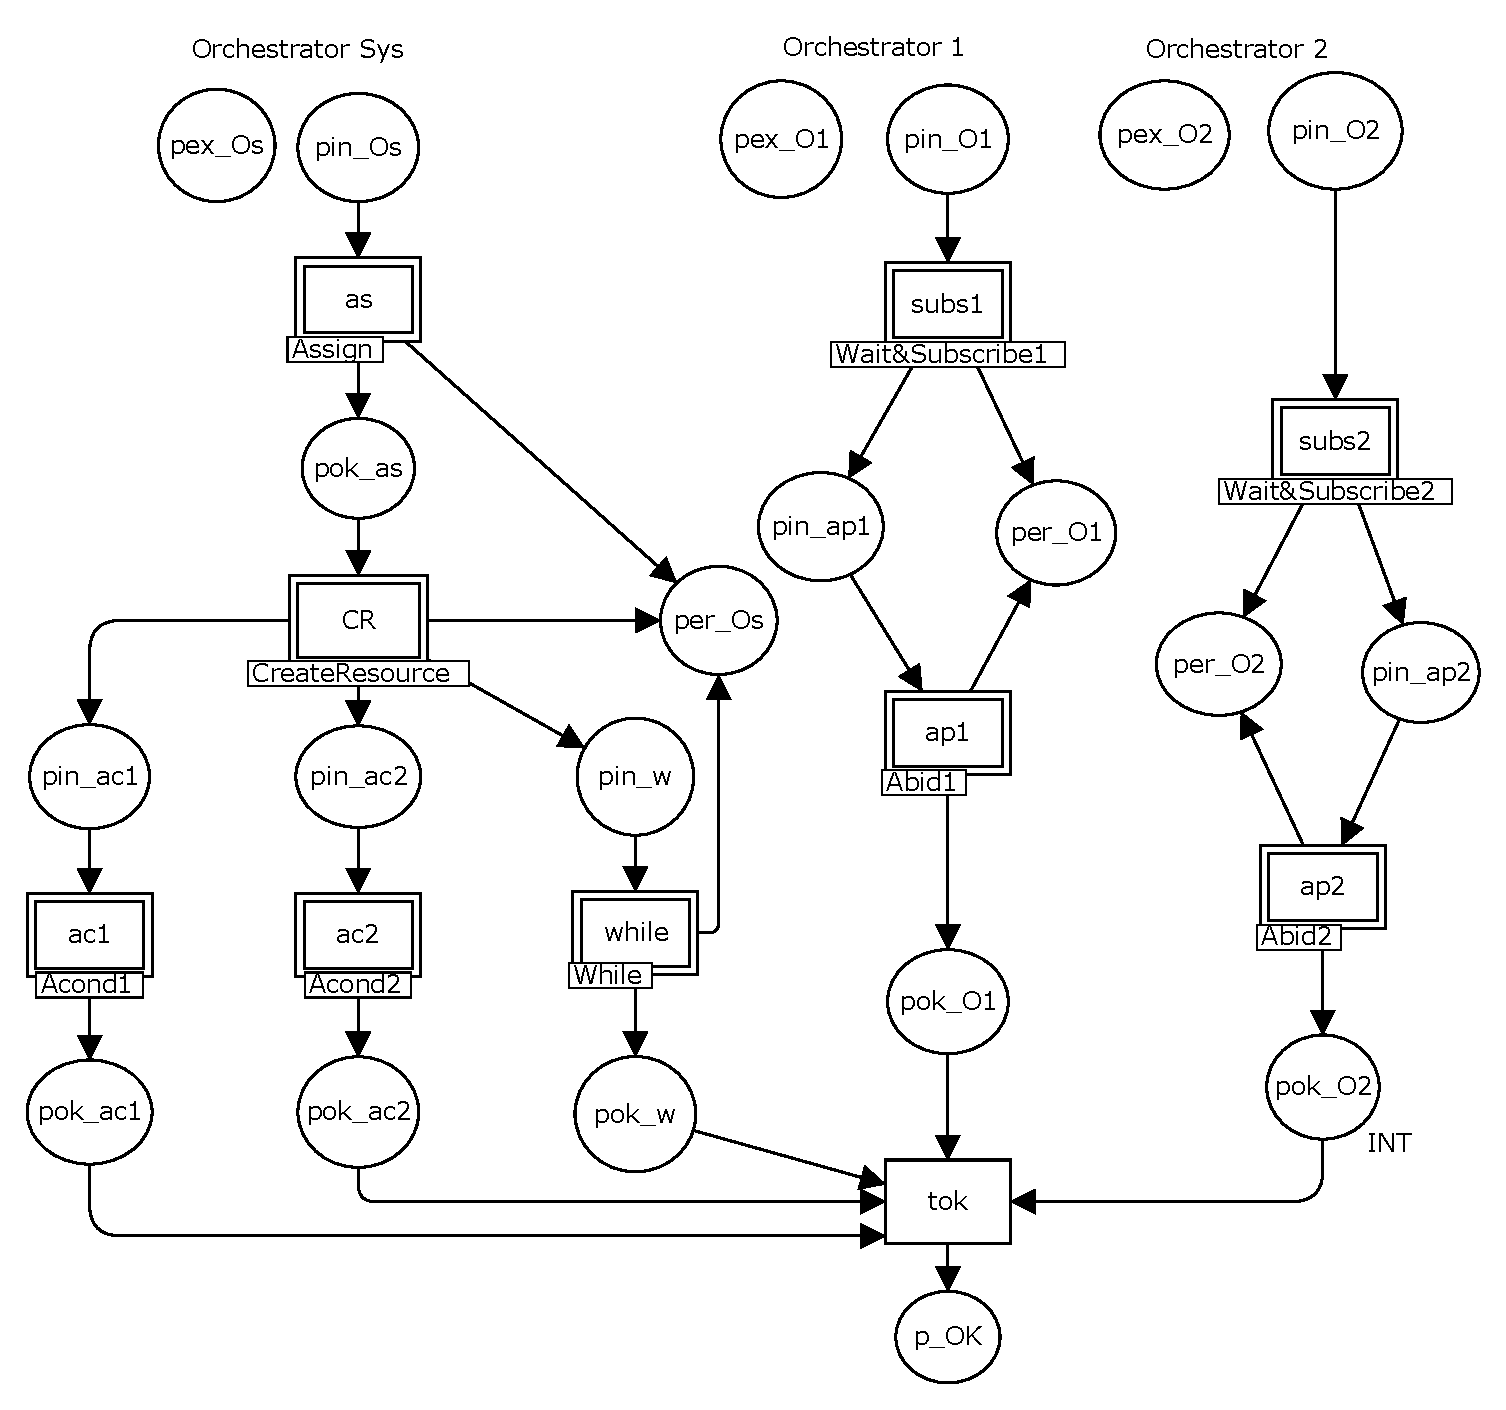
\includegraphics[scale=0.35]
{Figures/casestudy.eps}\end{center}}}
\end{center}
\vspace{-0.6cm}
\caption{\label{casestudy} A simplified PTCPN for the online auction system.}
\end{figure}

\section{Summary}\label{sumWebServ}
\markright{~\ref{sumWebServ} Summary}

This chapter has described a methodology called \textit{Correct-WS} for the design and verification of Web Service compositions and a tool called WST supporting several phases of this methodology. As a proof of concept the tool has been apply to an Internet purchase process case study. The chapter ends with a brief description of some parallel works which aim is also the development of correct Web Service compositions.

Although in this chapter sequence diagrams have been used to design the service composition behaviour in a proper way, sometimes we just have an electronic contract defining all the contractually correct behaviours of the system in a more general way. In these cases we would like to have a user-friendly representation of the e-contracts but having at the same time a formal background allowing us to verify the correctness of the e-contracts. That is what Chapter \ref{c4} is focused on.
\cleardoublepage

\chapter{Timed-arc workflow nets}\label{chapter:c4}
\markboth{Chapter~\ref{chapter:c4}. Contract-Oriented Diagrams (\codiag)}{}

%%This chapter presents a visual model for the representation of electronic contracts. It is based on a hierarchical tree diagram used to specify the contract clauses. We call this diagram \textit{Contract-Oriented Diagram} or \textit{C-O Diagram} for short. First, an informal description of the diagram is provided, describing the different elements that compose the model. Next, the diagram syntax and semantics are defined, where the semantics consists of a translation of the diagram into a network of timed automata, so the UPPAAL tool can be used for validation and verification of the e-contract model. A case study concerning an e-contract about an online auctioning process is presented, showing the usefulness of the approach. Finally, some alternative work related to \codiag\ is described.
%%
%%%%%Model description%%%
%%\section{\codiag\ Description}\label{Description}
%%\markright{~\ref{Description} \codiag\ Description}
%%
%%%%Basic Element%%
%%In Figure \ref{goal} we show the basic element of \codiag. It corresponds to a contract clause and we call it \textbf{box}. This box consists of four elements, allowing us to specify deontic norms, reparations and any restriction. There are also a name and an agent associated to the box. The \textit{name} is useful both to describe the clause and to reference the box from other clauses, so it cannot be repeated. The \textit{agent} can be used to indicate which one of the participants in the contract is affected by the clause in the box.
%%
%%\begin{figure}
%%\begin{center}
%%  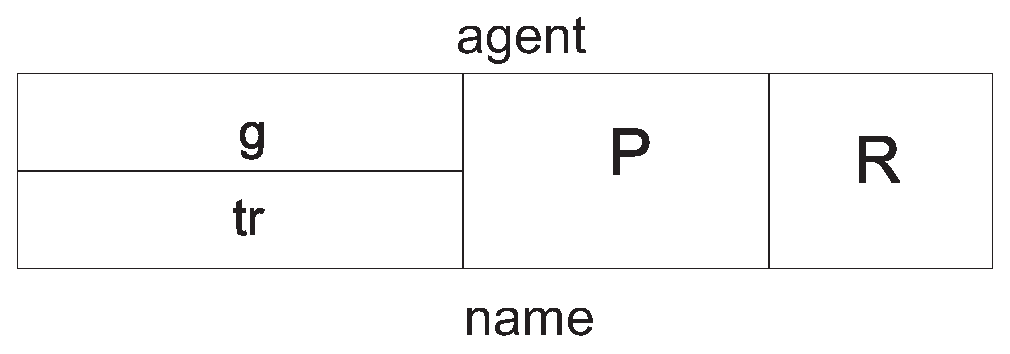
\includegraphics[width=7cm]{Figures/goal.eps}
%%\end{center}
%%  \caption{Box structure}
%%  \label{goal}
%%\end{figure}
%%
%%On the left-hand side of the box we specify the conditions and restrictions. The \textit{guard} \textbf{g} contains the conditions under which the contract clause must be taken into account. The \textit{time restriction} \textbf{tr} specifies the time frame in which the contract clause must be satisfied.
%%
%%The \textit{propositional content} \textbf{P}, on the centre, is the main element of the box, and it is used to specify deontic operators (obligations, permissions and prohibitions) that are applied over actions and the actions themselves.
%%
%%The last element of these boxes, on the right-hand side, is the \textit{reparation} \textbf{R}. This reparation, if specified by the contract clause, is another contract that must be satisfied in case the main norm is not satisfied, considering the clause eventually satisfied if this reparation is satisfied.
%%
%%%%Refinements%%
%%These basic elements of a \textit{C-O Diagram} can be refined by using AND/OR refinements, as shown in Figure \ref{refinem}, in the same way that we refine goals into subgoals in goal model diagrams \cite{Lamsweerde1993}. The aim of these refinements is to capture the hierarchical clause structure followed by most contracts. An \textbf{AND-refinement} means that all the subclauses must be satisfied in order to satisfied the parent clause. An \textbf{OR-refinement} means that it is only necessary to satisfy one of the subclauses in order to satisfy the parent clause, so we can choose which one to fulfil (exclusive or). In this way, we can build a hierarchical tree with the clauses defined by the contract, where the leaf clauses correspond to the atomic clauses, that is, to the clauses that cannot be divided into subclauses.
%%
%%\begin{figure}
%%\begin{center}
%%  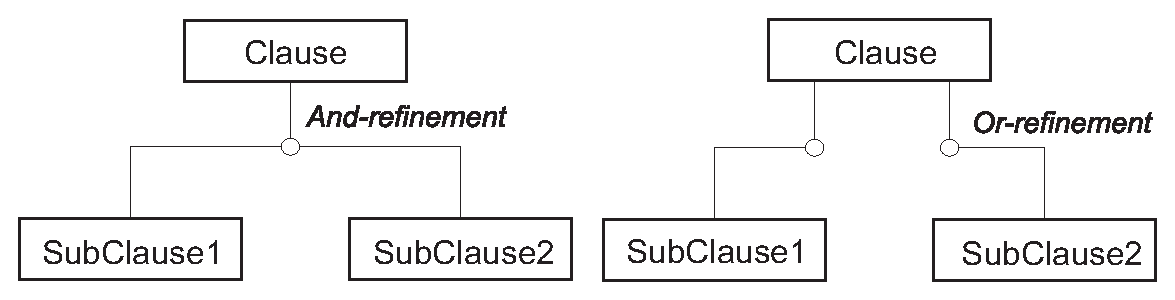
\includegraphics[width=10cm]{Figures/AndOrRefinement.eps}
%%\end{center}
%%  \caption{AND/OR refinements}
%%  \label{refinem}
%%\end{figure}
%%
%%It is also possible to use another refinement to specify a temporal relationship of sequence between the subclauses, as shown in Figure \ref{sequence}. We call it \textbf{SEQ-refinement} and it means that the norm specified in the target box (\textit{SubClause2} in Fig. \ref{sequence}) must be fulfilled after satisfying the norm specified in the source box (\textit{SubClause1} in Fig. \ref{sequence}).
%%
%%\begin{figure}
%%\begin{center}
%%  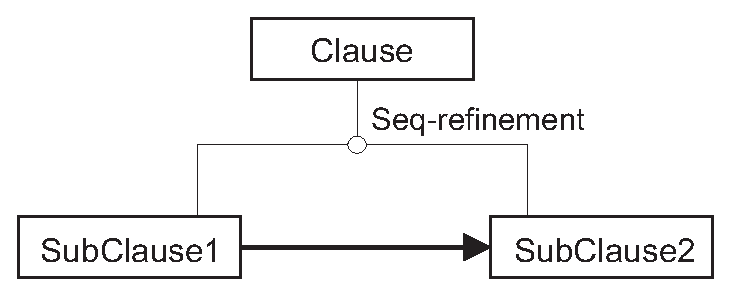
\includegraphics[width=7cm]{Figures/AndRefinementSequence.eps}
%%\end{center}
%%  \caption{Sequence refinement}
%%  \label{sequence}
%%\end{figure}
%%
%%Finally, there is another structure that can be used to model \textbf{repetition}, apart from the refinements previously defined. This structure is represented as an arrow going from a subclause to one of its ancestor clauses (or to itself), meaning the repetitive application of all the subclauses of the target clause after satisfying the source subclause. For example, in Figure \ref{Recursion} we have an \textbf{OR-refinement} with an arrow going from \textit{SubClause1} to \textit{Clause}. It means that after satisfying \textit{SubClause1} we apply \textit{Clause} again, but not after satisfying \textit{SubClause2}.
%%
%%\begin{figure}
%%\begin{center}
%%  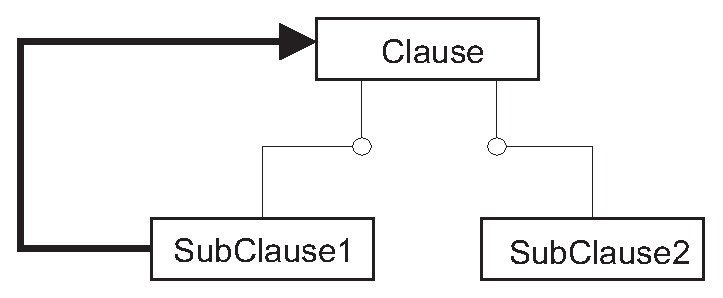
\includegraphics[width=7cm]{Figures/Recursion.eps}
%%\end{center}
%%  \caption{Repetition in \codiag}
%%  \label{Recursion}
%%\end{figure}
%%
%%%%Fields Description%%
%%In the next paragraphs we describe each one of the elements of a box/clause in more detail. For the sake of simplicity, we sometimes avoid writing all the elements of the boxes in the different figures, we just focus on the elements of interest in each case.
%%
%%\paragraph{\textbf{Propositional Content P}} This one is the main element of a box. It allows us to specify \textit{obligations}, \textit{permissions} and \textit{prohibitions} that the contract must satisfied. In this work, we follow an \textit{ought-to-do} approach \cite{Wright1999}, that is, these deontic operators are applied over \textit{actions} performed by the participants in the contract.
%%
%%We only consider the possibility of specifying \textit{atomic actions} in the \textbf{P} element of each one of the leaf clauses of our diagrams. These actions are denoted by lower case Latin letters (``a'',``b'',``c'', \ldots). We use a dash (``-'') to denote that there is no action specified in the no leaf clauses.
%%
%%The composition of actions can be achieved by means of the different kinds of refinement we have in \codiag. In this way, an AND-refinement can be used to model \textit{concurrency} ``\&'' between actions, an OR-refinement can be used to model a \textit{choice} ``+'' between actions, and a SEQ-refinement can be used to model \textit{sequence} ``;'' of actions. In Figure \ref{CompoundActions} we can see an example about how to model these compound actions through refinements, given two atomic actions \textit{a} and \textit{b}.
%%
%%\begin{figure}
%%\begin{center}
%%  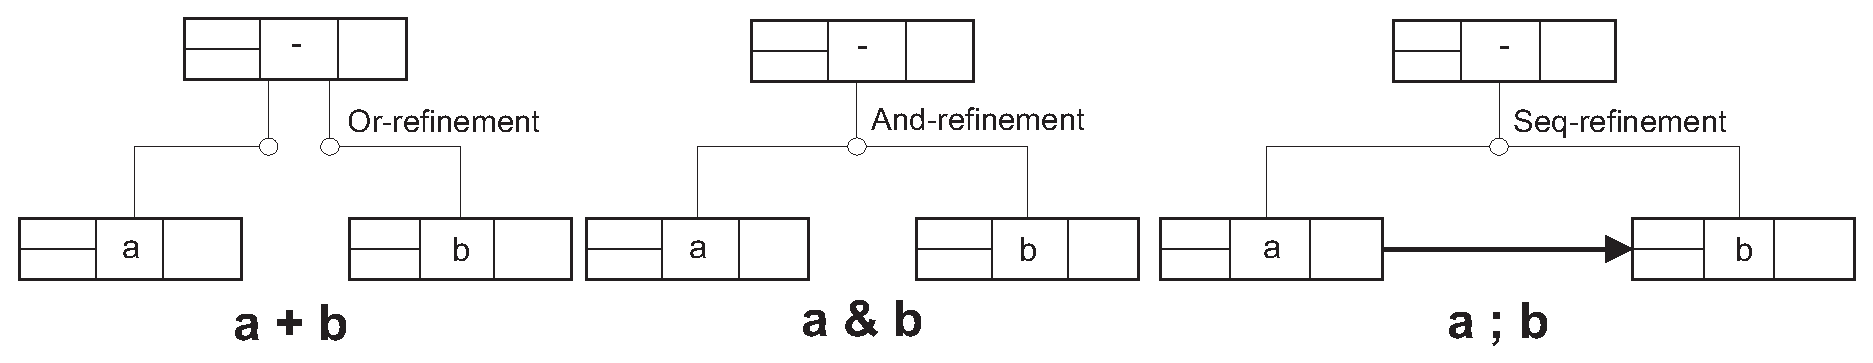
\includegraphics[width=12cm]{Figures/CompoundActions.eps}
%%\end{center}
%%  \caption{Compound actions in \codiag}
%%  \label{CompoundActions}
%%\end{figure}
%%
%%The \textit{deontic norms} (obligations, permissions and prohibitions) that are applied over these actions can be specified in any clause of our \codiag, affecting all the actions in the leaf clauses that are subclauses of this clause. If it is the case that the clause where we specify the deontic norm is a leaf clause, the norm only affects the atomic action we have in this clause. We use an upper case ``\textit{O}'' to denote an obligation, an upper case ``\textit{P}'' to denote a permission, and an upper case ``\textit{F}'' to denote a prohibition (forbidden). These letters are written in the top left corner of element \textbf{P} (Figure \ref{DeonticNorms}).
%%
%%\begin{figure}
%%\begin{center}
%%  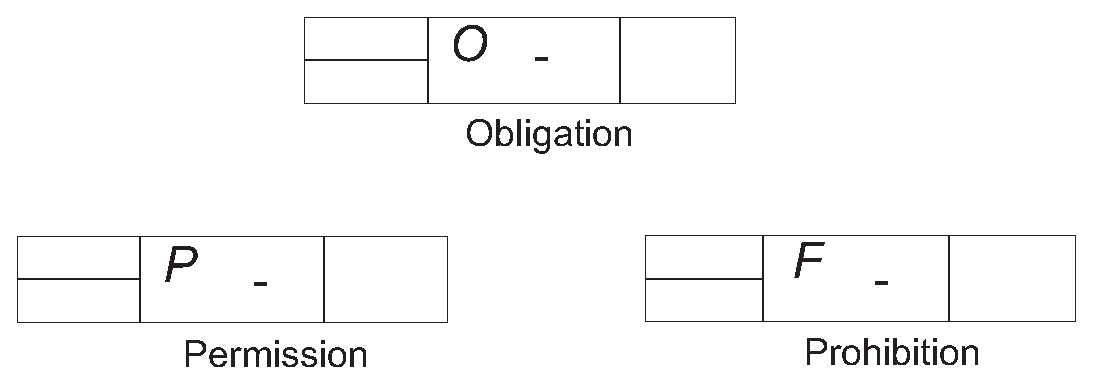
\includegraphics[width=8cm]{Figures/DeonticNorms.eps}
%%\end{center}
%%  \caption{Specification of deontic norms}
%%  \label{DeonticNorms}
%%\end{figure}
%%
%%The composition of deontic norms is also achieved by means of the different refinements we have in \codiag. Thus, an AND-refinement corresponds to the \textit{conjunction} operator ``$\wedge$'' between norms, an OR-refinement corresponds to the \textit{choice} operator ``$+$'' between norms, and a SEQ-refinement corresponds to the \textit{sequence} operator ``$;$'' between norms. For example, we can imagine having a leaf clause specifying the obligation of performing an action \textbf{a}, written as \textit{O}(a), and another leaf clause specifying the obligation of performing an action \textbf{b}, written as \textit{O}(b). These two norms can be combined in the three different ways mentioned before through the different kinds of refinement, as shown in Figure \ref{CompoundNorms}.
%%
%%\begin{figure}
%%\begin{center}
%%  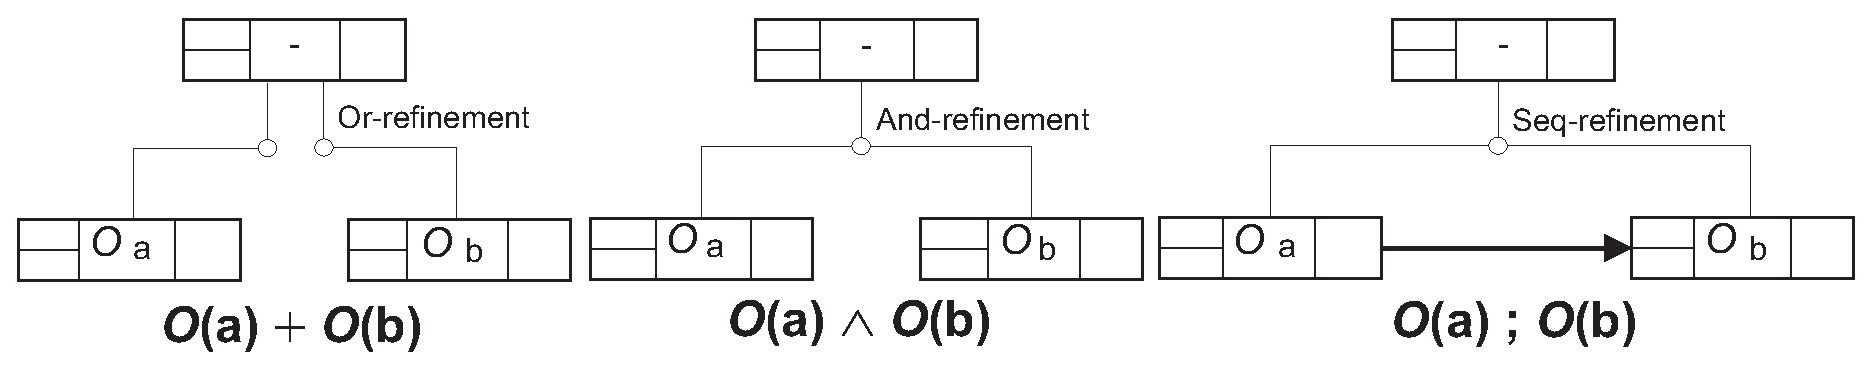
\includegraphics[width=12cm]{Figures/CompoundNorms.eps}
%%\end{center}
%%  \caption{Composition of deontic norms in \codiag}
%%  \label{CompoundNorms}
%%\end{figure}
%%
%%However, the specification of obligations, permissions and prohibitions in our diagrams must fulfil the following rules:
%%
%%{\renewcommand{\labelenumi}{\textit{\arabic{enumi}.}}
%%
%%\begin{enumerate}
%%
%%\item At least one deontic norm must be specified in each one of the branches of our hierarchical tree of clauses, i.e., we cannot have an action without a deontic norm applied over it.
%%
%%\item No more than one deontic norm can appear in each one of the branches of our hierarchical tree of clauses, i.e., we cannot have deontic norms applied over other deontic norms.
%%
%%\item The deontic norms we take into account to check restrictions \textit{1.} and \textit{2.} can be shared by several branches, i.e., when we have a deontic norm applied over a compound action, this norm is part of several branches of our hierarchical tree of clauses.
%%
%%\end{enumerate}
%%
%%}
%%
%%The \textit{repetition} of both, actions and deontic norms, can be achieved by means of the repetition structure we define in \codiag. The meaning of this structure is similar to the operator \textit{Kleene's star} ``$*$'' applied over the elements of the target clause of the arrow, but it is richer in the sense that the repetition can be conditioned to the satisfaction of the source clause of the arrow and not other alternative clause.
%%
%%To sum up, the content of element \textbf{P} in our \codiag\ change depending on the type of clause. In the \textit{leaf clauses} we must always specify an atomic action and we must also specify a deontic norm over this action if it has not been specified before in this branch of the diagram. In the \textit{no leaf clauses} we cannot specify actions, but we can specify a deontic norm whenever the rules listed before are not broken (there is not conflict with other norm and it is eventually applied over an action).
%%
%%\paragraph{\textbf{Reparation R}} This element of a box can state a \textit{new contract} that must be satisfied when the main proposition \textbf{P} is not satisfied (a \textit{prohibition} is violated or an \textit{obligation} is not fulfilled, there is not reparation for \textit{permission}). This new contract can be just a new norm, but it can also be a new hierarchical tree of clauses, including their own reparations. In this way, we are able to specify nested reparations in our \textit{C-O Diagram}.
%%
%%The element \textbf{R} is only allowed in the clauses of our diagrams where we specify a deontic norm of obligation or prohibition in element \textbf{P}, being forbidden in the rest of clauses. E.g., we can imagine a simple contract \textit{$C$} stating that we have the obligation of performing an atomic action \textit{a} and the prohibition of performing an atomic action \textit{b}. However, if we do not perform the obligatory action \textit{a}, we can compensate it by fulfilling another contract called \textit{$C_1$}, consisting of performing an action \textit{c} or an action \textit{d}, and if we perform the forbidden action \textit{b}, we can compensate it just by performing an action \textit{e}. This situation can be modelled in our diagrams as shown in Figure \ref{Reparations}.
%%
%%\begin{figure}
%%\begin{center}
%%  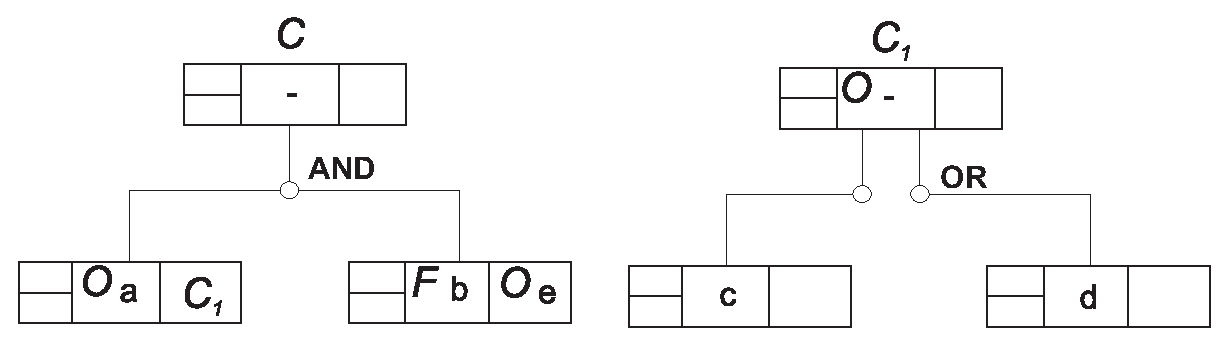
\includegraphics[width=10cm]{Figures/Reparations.eps}
%%\end{center}
%%  \caption{Reparations in \codiag}
%%  \label{Reparations}
%%\end{figure}
%%
%%At this point we can see clearly the difference between having a composition of obligations over atomic actions and having an obligation over a compound action. While the former allows us to specify a different reparation for each one of the atomic actions we are obliged to do, the latter only allows us to specify one reparation for the compound action that is under the obligation operator. For the first case, we can consider the diagrams we have in Figure \ref{CompoundNorms}, where it is possible to specify a different reparation in each one of the leaf clauses of the diagrams. For the second case, we can imagine having the diagrams shown in Figure \ref{ObligationCompoundActions}, where we can only specify reparations in the no leaf clauses where we have the obligations, covering these reparations the whole composition of actions.
%%
%%\begin{figure}
%%\begin{center}
%%  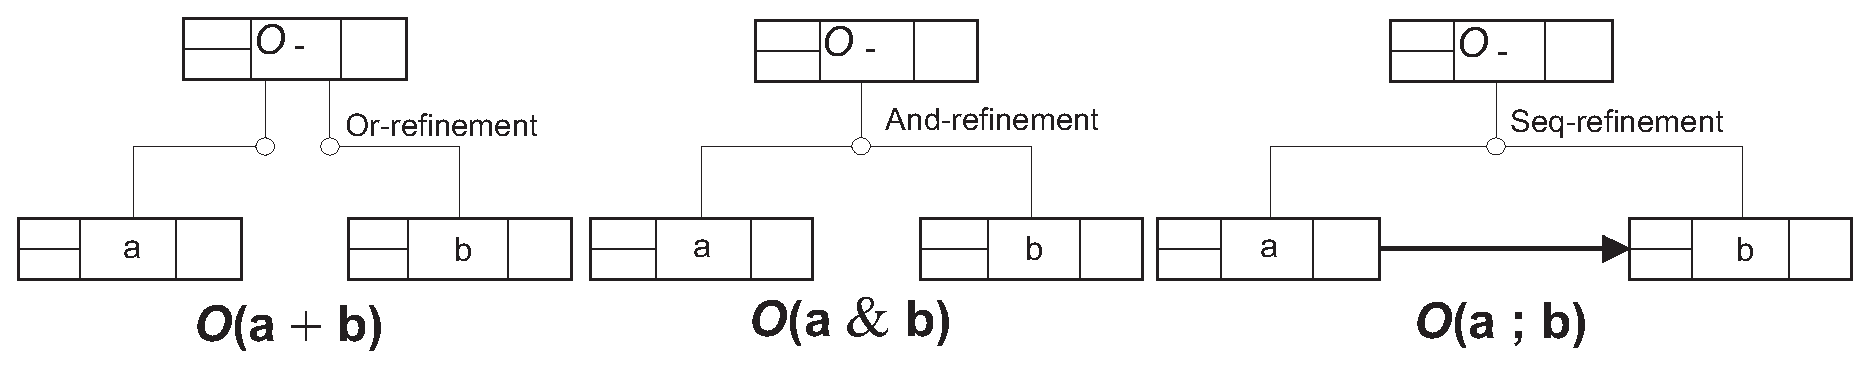
\includegraphics[width=12cm]{Figures/ObligationCompoundActions.eps}
%%\end{center}
%%  \caption{Obligations over compound actions}
%%  \label{ObligationCompoundActions}
%%\end{figure}
%%
%%This difference is a bit trickier if we consider prohibitions or permissions, because it not only concerns to the specification of reparations \cite{Pace2009}. For example, given two atomic actions \textit{a} and \textit{b}, the meaning of prohibiting the sequence of these two actions, written as \textit{F}(a$.$b), is different from the meaning of prohibiting action \textit{a}, and next prohibiting action \textit{b}, written as \textit{F}(a)$.$\textit{F}(b). In the first case, the sequence of actions starting with \textit{a} and continuing with any action different from \textit{b} is allowed, while in the second case any sequence of actions starting with \textit{a} is forbidden. In Figure \ref{ProhibitionActions} we can see how both cases are represented in our \codiag. Similar distinctions appear when we consider permissions instead of prohibitions.
%%
%%\begin{figure}
%%\begin{center}
%%  \includegraphics[width=12cm]{Figures/ProhibitionActions.eps}
%%\end{center}
%%  \caption{Prohibition of a sequence \textit{vs.} sequence of prohibitions}
%%  \label{ProhibitionActions}
%%\end{figure}
%%
%%\paragraph{\textbf{Guard g}} This element of a box is a \textit{boolean expression} that evaluates some information provided by the clause specification, telling us under which conditions the clause must be taken into account. For example, in a car insurance contract we can have a clause that is only applied to people who are under the age of 21. In that case, we must include in the box modelling this clause a guard similar to \textbf{age $<$ 21}, where \textbf{age} is a variable containing how old the client is and \textbf{21} is an integer value.
%%
%%Basically, a guard is a set of expressions that evaluate to a boolean (\textit{true} or \textit{false}) combined by means of conjunctions (\textit{and}), disjunctions (\textit{or}), and negations (\textit{not}). These expressions can include constant values, variables, and equality and inequality operators (\textit{$==$},\textit{$!=$},\textit{$<$},\textit{$>$}, \ldots). 
%%
%%The interpretation of these guards within the different kinds of refinement is the following:
%%
%%\begin{itemize}
%%
%%\item When the guard condition corresponding to a subclause of an \textbf{AND-refinement} or a \textbf{SEQ-refinement} evaluates to \textit{false}, the subclause is trivially satisfied, so we only must check the subclauses with a \textit{true} guard (or without guard).
%%
%%\item When the guard condition corresponding to a subclause of an \textbf{OR-refinement} evaluates to \textit{false}, we cannot satisfy that subclause in order to satisfy the parent clause, so it is necessary to satisfy one of the other subclauses with a \textit{true} guard (or without guard).
%%
%%\end{itemize}
%%
%%\paragraph{\textbf{Time restriction tr}} This element allows us to include timing aspects in the boxes of our diagram. In this way, we can associate deadlines, timeouts, etc. to the clauses of our contract. These real-time aspects are expressed in the boxes of our diagram by means of \textit{intervals} within \textbf{tr}. These intervals indicate the period of time in which the clauses must be satisfied.
%%
%%The time restrictions can be specified in two different ways within the boxes: we can specify the \textit{dates} binding the beginning and the end of the time frame corresponding to the clause (\textit{absolute time}), or we can specify a deadline saying the number of \textit{time units} that can elapse before the clause is satisfied from the moment at which another clause is satisfied or from the moment at which the contract comes into effect (\textit{relative time}). 
%%
%%For example, in the case of absolute time, we can model a contract stating that a clause must be satisfied in the \textbf{first five days of October}, as shown on the top of Figure \ref{TimeIntervals} (a). In the case of relative time, a contract can state that a clause must be satisfied not later than \textbf{five days after satisfying other clause}, as shown on the bottom of Figure \ref{TimeIntervals} (b), where \textit{SubClause3} must be satisfied before five days after satisfying \textit{SubClause1} (abridged as \textit{S.C.1}).
%%
%%\begin{figure}
%%\begin{center}
%%  \includegraphics[width=12cm]{Figures/TimeIntervals.eps}
%%\end{center}
%%  \caption{\codiag\ with time restrictions}
%%  \label{TimeIntervals}
%%\end{figure}
%%
%%When we have a time restriction specified in a clause of the diagram that is refined into subclauses, this restriction affects all the subclauses. That is, all the subclauses necessary to satisfy the parent clause must be satisfied in the time frame specified in this parent clause. Otherwise, the parent clause is considered unfulfilled.
%%
%%%%Evaluation of the model%%
%%\subsection{Evaluation of the Model}
%%
%%%%Qualitative evaluation%%
%%In this subsection we present a qualitative evaluation of the visual model proposed for the description of electronic contracts. For this evaluation we discuss how the model fits some of the most important principles for designing effective visual notations defined in \cite{Moody2009}.
%%
%%First, the principle of \textit{semiotic clarity} is accomplished by the model, as there is only one graphical structure corresponding to each semantic concept and vice versa.
%%
%%Second, the principle of \textit{perceptual discriminability} is taken into account to differentiate between refinements, having each kind of refinement a clearly distinct shape and using the text with the name of the refinement to complement the graphics (principle of \textit{dual coding}).
%%
%%We also have that the number of different graphical symbols in the model is under the upper limit of six categories for graphics complexity, so the principle of \textit{graphic economy} is accomplished.
%%
%%Finally, the principle of \textit{complexity management} is covered by the modularization of the diagrams, where different modules can be integrated by means of a same box appearing in several diagrams (principle of \textit{cognitive integration}).
%%
%%%%%Model syntax%%%
%%\section{\codiag\ Syntax}\label{Syntax}
%%\markright{~\ref{Syntax} \codiag\ Syntax}
%%
%%\bdfn\label{defCOSyntax} (C-O Diagrams Syntax) \\
%%
%%We consider a finite set of real-valued variables $\mathcal{C}$ standing for clocks, a finite set of non-negative integer-valued variables $\mathcal{V}$, a finite alphabet $\Sigma$ for atomic actions, a finite set of identifiers $\mathcal{A}$ for agents, and another finite set of identifiers $\mathcal{N}$ for names. The Greek letter $\epsilon$ means that an expression is not given, i.e., it is empty.
%%
%%We use $C$ to denote the contract modelled by a \textit{C-O Diagram}. The diagram is defined by the following EBNF grammar:
%%
%%\begin{center}
%%\begin{tabular}{rcl}
%%    $C$ & $:=$ &  \begin{array}[t]{l}
%%						      (agent,name,g,tr,O(C_2),R) \,|\,
%%									(agent,name,g,tr,P(C_2),\epsilon) \,|\,	      
%%						      \end{array} \\    
%%		&  &  \begin{array}[t]{l}		      
%%		      (agent,name,g,tr,F(C_2),R) \,|\,
%%					(\epsilon,name,g,tr,C_1,\epsilon)
%%		      \end{array} \\		
%%    $C_1$ & $:=$ &  \begin{array}[t]{l}
%%								      C \,(And \; C)^+\,|\,
%%								      C \,(Or \; C)^+\,|\,
%%								      C \,(Seq \; C)^+
%%								      \end{array} \\
%%		$C_2$ & $:=$ &  \begin{array}[t]{l}
%%											a \,|\,
%%								      C_3 \,(And \; C_3)^+\,|\,
%%								      C_3 \,(Or \; C_3)^+\,|\,
%%								      C_3 \,(Seq \; C_3)^+
%%								      \end{array} \\
%%    $C_3$ & $:=$ &  \begin{array}[t]{l}
%%								      (\epsilon,name,\epsilon,\epsilon,C_2,\epsilon)								      
%%								      \end{array} \\
%%		$R$ & $:=$ &  \begin{array}[t]{l}
%%						      C \,|\,
%%						      \epsilon
%%						      \end{array} \\		
%%\end{tabular}
%%\end{center}
%%\noindent where $a \in \Sigma$, $agent \in \mathcal{A}$ and $name \in \mathcal{N}$. Guard $g$ is $\epsilon$ or a conjunctive formula of atomic constraints of the form: $v \sim n$ or $v - w \sim n$, for $v,w\in \mathcal{V}$, $\sim \in \{\, \leq, <, =, >, \geq \, \}$ and $n \in \nat$, whereas timed restriction $tr$ is $\epsilon$ or a conjunctive formula of atomic constraints of the form: $x \sim n$ or $x -y \sim n$, for $x,y \in \mathcal{C}$, $\sim \in \{\, \leq, <, =, >, \geq \, \}$ and $n \in \nat$. $O$, $P$ and $F$ are the deontic operators corresponding to obligation, permission and prohibition, respectively, where $O(C_2)$ states the obligation of performing $C_2$, $F(C_2)$ states prohibition of performing $C_2$, and $P(C_2)$ states the permission of performing $C_2$. $And$, $Or$ and $Seq$ are the operators corresponding to the refinements we have in \codiag, AND-refinement, OR-refinement and SEQ-refinement, respectively.
%%
%%\edfn
%%
%%The most simple contract we can have in \codiag\ is that composed of only one box including the elements $agent$ and $name$. Optionally, we can specify a guard $g$ and a time restriction $tr$. We also have a deontic operator ($O$, $P$ or $F$) applied over an atomic action $a$, and in the case of obligations and prohibitions it is possible to specify another contract $C$ as a reparation. E.g., $C:=(Buyer,Example1,\epsilon,\epsilon,O(pay),C^\prime)$ (Figure \ref{GrammarExamples}, on the bottom left) is a very simple contract specifying for a buyer the obligation of paying, otherwise contract $C^\prime$ comes into effect.
%%
%%We use $C_1$ to define a more complex contract where we combine different deontic norms by means of any of the different refinements we have in \codiag. In the box where we have the refinement into $C_1$ we cannot specify an agent nor a reparation because these elements are always related to a single deontic norm, but we still can specify a guard $g$ and a time restriction $tr$ that affect all the deontic norms we combine. E.g., $C:=(\epsilon,Example2,\epsilon,x<5,C^\prime \, Or \, C^{\prime\prime},\epsilon)$ (Figure \ref{GrammarExamples}, on the top left) is a composed contract specifying that contract $C^\prime$ or contract $C^{\prime\prime}$ must be satisfied in order to satisfy $C$ within 5 time units.
%%
%%Once we write a deontic operator in a box of our diagram, we have two possibilities as we can see in the specification of $C_2$: we can just write a simple action $a$ in the box, being the deontic operator applied only over it, or we can refine this box in order to apply the deontic operator over a compound action. In this case we have that the subboxes ($C_3$) cannot define a new deontic operator as it has already been defined in the parent box (affecting all the subboxes). Then, these subboxes cannot specify an agent nor a reparation. For example, $C:=(Buyer,Example3,\epsilon,\epsilon,O(C^\prime \, Or \, C^{\prime\prime}),\epsilon)$, where we have that $C^\prime:=(\epsilon,Option1,\epsilon,\epsilon,pay\_cash,\epsilon)$ and $C^{\prime\prime}:=(\epsilon,Option2,\epsilon,\epsilon,pay\_card,\epsilon)$ (Figure \ref{GrammarExamples}, on the right), is a contract specifying for a buyer the obligation of paying by cash or by credit card.
%%
%%\begin{figure}
%%\begin{center}
%%  \includegraphics[width=9cm]{Figures/GrammarExamples.eps}
%%\end{center}  
%%  \caption{Syntax examples}
%%  \label{GrammarExamples}
%%\end{figure}
%%
%%%%%Model semantics%%%
%%\section{\codiag\ Semantics}\label{Semantics}
%%\markright{~\ref{Semantics} \codiag\ Semantics}
%%
%%%%Timed automata extensions for the model%%
%%The \codiag\ semantics is defined by means of a transformation into an NTA, adding the definition of two orderings, $\prec_N$ and $\prec_E$, where:
%%
%%\begin{itemize}
%%
%%\item $\prec_N$ is a (strict, partial) ordering on N where $n \prec_N n'$ means that node $n$ is better than node $n'$.
%%
%%\item $\prec_E$ is a (strict, partial) ordering on E where $e \prec_N e'$ means that edge $e$ is better than edge $e'$.
%%
%%\end{itemize}
%%
%%We also add a \textbf{violation set} $V(n)$ associated to each node $n$ in $N$, that is the set of contractual norms that are violated in $n$.
%%
%%\bdfn\label{defVio} (Violation Set) \\
%%
%%Let us consider the set of contractual norms $\mathcal{CN}$ ranged over $cn$, $cn'$, \ldots\ standing for identifiers of norms. We write $n \not \models cn$ to express that norm $cn$ is violated in node $n$. Therefore, the violation set is defined as $V(n)=\{cn \, | \, cn \in \mathcal{CN}$ and  $n \not \models cn\}$.
%%
%%\edfn
%%
%%Another set called \textbf{satisfaction set} $S(n)$ is also associated to each node $n$ in $N$. This set is composed by the contractual obligations and prohibitions that have already been satisfied in $n$. 
%%
%%\bdfn\label{defSat} (Satisfaction Set) \\
%%
%%Let us consider the set of contractual obligations and prohibitions $\mathcal{COF}$ ranged over $cof$, $cof'$, \ldots\ standing for identifiers of obligations and prohibitions. We write $n \models cof$ to express that obligation or prohibition $cof$ has been satisfied in node $n$ (we consider a prohibition satisfied in node $n$ if it has not been violated and cannot be violated anymore). Hence, the satisfaction set is defined as $S(n)=\{cof \, | \, cof \in \mathcal{COF}$ and  $n \models cof\}$.
%%
%%\edfn
%%
%%Once these two sets have been defined, we can formally define the \textbf{ordering on nodes} $\prec_N$, by comparing the violation sets and the satisfaction sets of the nodes, and the \textbf{ordering on edges} $\prec_E$, by comparing the violation sets and the satisfaction sets of the target nodes of the edges.
%%
%%\bdfn\label{defOrdN} (Ordering on Nodes) \\
%%
%%A node $n_1$ is better than another node $n_2$ if the violation set of $n_1$ is a proper subset of the violation set of $n_2$ or, if the violation sets are the same, a node $n_1$ is better than another node $n_2$ if the satisfaction set of $n_1$ is a proper superset of the satisfaction set of $n_2$, that is, $n_1 \prec_N n_2$ iff $(V(n_1) \subset V(n_2))$ or $(V(n_1) = V(n_2)$ and $S(n_1) \supset S(n_2))$.
%%
%%\edfn
%%
%%\bdfn\label{defOrdE} (Ordering on Edges) \\
%%
%%An edge $e_1$ is better than another edge $e_2$ if the source node is the same in both cases but the violation set of the target node of $e_1$ is a proper subset of the violation set of the target node of $e_2$ or, if the violation sets are the same, an edge $e_1$ is better than another edge $e_2$ if the satisfaction set of the target node of $e_1$ is a proper superset of the satisfaction set of the target node of $e_2$. Considering $e_1=(n_1,g_1,a_1,s_1,r_1,n{_1}')$ and $e_2=(n_2,g_2,a_2,s_2,r_2,n{_2}')$, $e_1 \prec_E e_2$ iff $(n_1=n_2)$ and $(V(n{_1}') \subset V(n{_2}')$ or $(V(n{_1}') = V(n{_2}')$ and $S(n{_1}') \supset S(n{_2}')))$.
%%
%%\edfn
%%
%%Finally, another set called \textbf{permission set} $P(n)$ is associated to each node $n$ in $N$. This set influences neither the ordering on nodes nor the ordering on edges, it is used just to record the permissions in the contract that have been made effective.
%%
%%\bdfn\label{defPer} (Permission Set) \\
%%
%%Let us consider the set of contractual permissions $\mathcal{CP}$ ranged over $cp$, $cp'$,\ldots\ standing for identifiers of permissions. We write $n \models cp$ to express that permission $cp$ has already been made effective in node $n$. Then, the permission set is defined as $P(n)=\{cp \, | \, cp \in \mathcal{CP}$ and  $n \models cp\}$.
%%
%%\edfn
%%
%%Graphically, when we draw a timed automaton extended with these three sets, we write under each node $n$ between braces its violation set $V(n)$ on the left, its satisfaction set $S(n)$ on the centre and its permission set $P(n)$ on the right. In the initial node of the automata we build corresponding to \codiag\ these three sets are empty. By default, a node keep in these sets the same content of the previous node. Only in a few cases the content of these sets is modified (when an obligation or a prohibition is violated, an obligation or a prohibition is satisfied or a permission is made effective).
%%
%%%%Time issues%%
%%Concerning the \textbf{real-time restrictions} $tr$ specified in the contract, the two types of time restrictions we can have in \codiag\ must be translated in a different way for their inclusion into a timed automaton construction:
%%
%%\begin{itemize}
%%
%%\item A time restriction specified using \textbf{absolute time} must be specified in timed automata by rewriting the terms in which absolute time references occur. For that purpose we define a global clock $T \in \mathcal{C}$ that is never reset during the execution of the automata and, taking into account the moment at which the contract is enacted, we rewrite the absolute time references as deadlines involving clock $T$ and considering the smallest time unit needed in the contract. For example, let us consider a clause that must be satisfied between the \textit{5th of November} and the \textit{10th of November}, and that the contract containing this clause is enacted the \textit{31st of October}. If we suppose that \textit{days} is the smallest time unit used in the contract for the specification of real-time restrictions, the time restriction of this clause is written as $(T \geq 5) \, and \, (T \leq 10)$.
%%
%%\item A time restriction specified using \textbf{relative time} must be specified in timed automata by introducing an additional clock to register the amount of time that has elapsed since another clause has been satisfied, resetting the additional clock value when this happens and specifying the deadline using it. We call this clock $t_{name}$, where $name$ is the clause used as reference for the specification of the time restriction. Therefore, we define a set of additional clocks $C_{add}=\{t_{name} \, | \,  t_{name} \in \mathcal{C}\}$ including a clock for every clause that is used as reference in the time restriction of at least another clause. For example, let us consider a contract with a clause that must be satisfied between \textit{5} and \textit{10} days after another clause $name1$ has been satisfied. In this case we define an additional clock $t_{name1}$ that is reset to zero when clause $name1$ is satisfied ($t_{name1}:=0$) and the time restriction of the other clause is written as $(t_{name1} \geq 5) \, and \, (t_{name1} \leq 10)$.
%%
%%\end{itemize}
%%
%%As a result, the set of clocks of the timed automata would be $\mathcal{C} = \{T\} \cup C_{add}$. When we construct the timed automata corresponding to \codiag, we always consider $(x \geq t1) \, and \, (x \leq t2)$ as the interval corresponding to the time restriction $tr$ of the clause, where $x \in \mathcal{C}$ is the clock used for its specification ($x=T$ in the case of absolute time and $x=t_{name}$ in the case of relative time, being $name$ the clause used as reference), $t1 \in \nat$ is the beginning of the interval and $t2 \in \nat$ is the end of the interval ($t1 \leq t2$). If $tr$ does not define the lower bound of the interval we take $t1=0$, if $tr$ does not define the upper bound of the interval we take $t2=\infty$, and if $tr = \epsilon$ we take $t1=0$, $t2=\infty$ and $x=T$.
%%
%%%%Timed automata construction rules%%
%%Once we have given these extensions of the definition of timed automata and we have explained how the different kinds of time restriction can be expressed, considering all the different elements we can specify in a \textit{C-O Diagram}, we can define the transformation of the diagrams into timed automata by induction using several transformation rules.
%%
%%\bdfn\label{defTR} (\codiag\ Transformation Rules: Part I)\\
%%
%%{\renewcommand{\labelenumi}{(\arabic{enumi})}
%%\begin{enumerate}
%%
%%%1
%%\item An \textbf{atomic action} in a \textit{C-O Diagram}, that is, $(\epsilon,name,\epsilon,\epsilon,a,\epsilon)$ corresponds to the timed automaton $\mathcal{A}=(N_{\mathcal{A}}, n_{0_{\mathcal{A}}}, E_{\mathcal{A}}, I_{\mathcal{A}})$, where:
%%
%%\begin{itemize}
%%
%%\item $N_{\mathcal{A}}=\{a_{init},a_{end}\}$.
%%
%%\item $n_{0_{\mathcal{A}}}=a_{init}$.
%%
%%\item $E_{\mathcal{A}}=\{a_{init} \flechald{a}{} a_{end}\}$.
%%
%%\item $I_{\mathcal{A}}=\emptyset$.
%%
%%\end{itemize}
%%
%%The violation (\textbf{V}), satisfaction (\textbf{S}) and permission (\textbf{P}) sets are not modified, so $V(a_{init})=V(a_{end})$, $S(a_{init})=S(a_{end})$ and $P(a_{init})=P(a_{end})$. This timed automaton can be seen in Figure \ref{automaton_A1}.
%%
%%\begin{figure}
%%\begin{center}
%%  \includegraphics[width=5cm]{Figures/automaton_a1.eps}
%%\end{center}
%%  \caption{Automaton corresponding to a \textbf{simple action} $a$}
%%  \label{automaton_A1}
%%\end{figure}
%%
%%\separ
%%
%%%2
%%\item A \textbf{compound action} in a \textit{C-O Diagram} where an \textbf{AND-refinement} is used to compose actions, that is, $(\epsilon,name,\epsilon,\epsilon,C_1 \, And \, C_2 \, And \ldots And \, C_n,\epsilon)$ corresponds to the cartesian product of the automata corresponding to each one of the subcontracts. Let us consider $\mathcal{A}, \mathcal{B}, \ldots, \mathcal{Z}$ the automata corresponding to the subcontracts $C_1, C_2, \ldots, C_n$ (the actions specified in these subcontracts can be atomic actions or other compound actions). The resulting automaton $\mathcal{AND}$ corresponds to the cartesian product of these automata, that is, $\mathcal{AND} = \mathcal{A} \times \mathcal{B} \times \ldots \times \mathcal{Z}$. Again, the violation (\textbf{V}), satisfaction (\textbf{S}) and permission (\textbf{P}) sets are not modified, so they are the same in all the nodes. This composition of timed automata is shown graphically in Figure \ref{automaton_A2}.
%%
%%\begin{figure}
%%\begin{center}
%%  \includegraphics[width=12cm]{Figures/automaton_a2.eps}
%%\end{center}
%%  \caption{Automaton corresponding to a \textbf{compound action} (AND-refinement)}
%%  \label{automaton_A2}
%%\end{figure}
%%
%%\separ
%%
%%%3
%%\item A \textbf{compound action} in a \textit{C-O Diagram} where an \textbf{OR-refinement} is used to compose actions, that is, $(\epsilon,name,\epsilon,\epsilon,C_1 \, Or \, C_2 \, Or \ldots Or \, C_n,\epsilon)$ corresponds to a new automaton in which the automata corresponding to each one of the subcontracts is considered as an alternative. Let us consider $\mathcal{A}, \mathcal{B}, \ldots, \mathcal{Z}$ the automata corresponding to the subcontracts $C_1, C_2, \ldots, C_n$ (the actions specified in these subcontracts can be atomic actions or other compound actions). The resulting automaton $\mathcal{OR}$ preserves the structure of the automata we are composing but adding a new initial node $OR_{init}$ and connecting this node by means of urgent edges performing no action to the initial nodes of $\mathcal{A}, \mathcal{B}, \ldots, \mathcal{Z}$ ($A_{init}, B_{init}, \ldots, Z_{init}$). It is also added a new ending node $OR_{end}$ and urgent edges performing no action from the ending nodes of $\mathcal{A}, \mathcal{B}, \ldots, \mathcal{Z}$ ($A_{end}, B_{end}, \ldots, Z_{end}$) to this new ending node. Let $\mathcal{A}=(N_{\mathcal{A}}, n_{0_{\mathcal{A}}}, E_{\mathcal{A}}, I_{\mathcal{A}}), \mathcal{B}=(N_{\mathcal{B}}, n_{0_{\mathcal{B}}}, E_{\mathcal{B}}, I_{\mathcal{B}}), \ldots, \mathcal{Z}=(N_{\mathcal{Z}}, n_{0_{\mathcal{Z}}}, E_{\mathcal{Z}}, I_{\mathcal{Z}})$. The resulting automaton is therefore $\mathcal{OR}=(N_{\mathcal{OR}}, n_{0_{\mathcal{OR}}}, E_{\mathcal{OR}}, I_{\mathcal{OR}})$, where:
%%
%%\begin{itemize}
%%
%%\item $N_{\mathcal{OR}}=N_{\mathcal{A}} \cup N_{\mathcal{B}} \cup \ldots \cup N_{\mathcal{Z}}\cup \{OR_{init},OR_{end}\}$.
%%
%%\item $n_{0_{\mathcal{OR}}}=OR_{init}$.
%%
%%\item $E_{\mathcal{OR}}=E_{\mathcal{A}} \cup E_{\mathcal{B}} \cup \ldots \cup E_{\mathcal{Z}} \cup \{OR_{init} \flechalu{}{} A_{init}, OR_{init} \flechalu{}{} B_{init}, \ldots,$\\
%%$OR_{init} \flechalu{}{} Z_{init}\} \cup \{A_{end} \flechalu{}{} OR_{end}, B_{end} \flechalu{}{} OR_{end}, \ldots,$\\
%%$Z_{end} \flechalu{}{} OR_{end}\}$.
%%
%%\item $I_{\mathcal{OR}}=I_{\mathcal{A}} \cup I_{\mathcal{B}} \cup \ldots \cup I_{\mathcal{Z}}$.
%%
%%\end{itemize}
%%
%%The violation (\textbf{V}), satisfaction (\textbf{S}) and permission (\textbf{P}) sets are not modified, so they are the same in all the nodes. This composition of timed automata is shown graphically in Figure \ref{automaton_A3}.
%%
%%\begin{figure}
%%\begin{center}
%%  \includegraphics[width=7cm]{Figures/automaton_a3.eps}
%%\end{center}
%%  \caption{Automaton corresponding to a \textbf{compound action} (OR-refinement)}
%%  \label{automaton_A3}
%%\end{figure}
%%
%%\separ
%%
%%%4
%%\item A \textbf{compound action} in a \textit{C-O Diagram} where a \textbf{SEQ-refinement} is used to compose actions, that is, $(\epsilon,name,\epsilon,\epsilon,C_1 \, Seq \, C_2 \, Seq \ldots Seq \, C_n,\epsilon)$ corresponds to a new automaton in which the automata corresponding to each one of the subcontracts are connected in sequence. Let us consider $\mathcal{A}, \mathcal{B}, \ldots, \mathcal{Z}$ the automata corresponding to the subcontracts $C_1, C_2, \ldots, C_n$ (the actions specified in these subcontracts can be atomic actions or other compound actions). The resulting automaton $\mathcal{SEQ}$ preserves the structure of the automata we are composing, adding no extra nodes. We only connect with an urgent edge performing no action the ending node of each automaton in the sequence ($A_{end}, B_{end}, \ldots, Y_{end}$) with the initial node of the next automaton in the sequence ($B_{init}, C_{init}, \ldots, Z_{init}$). This rule is not applied in the cases of $A_{init}$ (as there is not previous ending node to connect) and $Z_{end}$ (as there is not following initial node to connect). Let $\mathcal{A}=(N_{\mathcal{A}}, n_{0_{\mathcal{A}}}, E_{\mathcal{A}}, I_{\mathcal{A}}), \mathcal{B}=(N_{\mathcal{B}}, n_{0_{\mathcal{B}}}, E_{\mathcal{B}}, I_{\mathcal{B}}), \ldots, \mathcal{Z}=(N_{\mathcal{Z}}, n_{0_{\mathcal{Z}}}, E_{\mathcal{Z}}, I_{\mathcal{Z}})$. The resulting automaton is therefore $\mathcal{SEQ}=(N_{\mathcal{SEQ}}, n_{0_{\mathcal{SEQ}}}, E_{\mathcal{SEQ}}, I_{\mathcal{SEQ}})$, where:
%%
%%\begin{itemize}
%%
%%\item $N_{\mathcal{SEQ}}=N_{\mathcal{A}} \cup N_{\mathcal{B}} \cup \ldots \cup N_{\mathcal{Z}}$.
%%
%%\item $n_{0_{\mathcal{SEQ}}}=A_{init}$.
%%
%%\item $E_{\mathcal{SEQ}}=E_{\mathcal{A}} \cup E_{\mathcal{B}} \cup \ldots \cup E_{\mathcal{Z}} \cup \{A_{end} \flechalu{}{} B_{init}, B_{end} \flechalu{}{} C_{init}, \ldots,$\\
%%$Y_{end} \flechalu{}{} Z_{init}\}$.
%%
%%\item $I_{\mathcal{SEQ}}=I_{\mathcal{A}} \cup I_{\mathcal{B}} \cup \ldots \cup I_{\mathcal{Z}}$.
%%
%%\end{itemize}
%%
%%Again, the violation (\textbf{V}), satisfaction (\textbf{S}) and permission (\textbf{P}) sets are not modified, so they are the same in all the nodes. This composition of timed automata is shown graphically in Figure \ref{automaton_A4}.
%%
%%\begin{figure}
%%\begin{center}
%%  \includegraphics[width=12cm]{Figures/automaton_a4.eps}
%%\end{center}
%%  \caption{Automaton corresponding to a \textbf{compound action} (SEQ-refinement)}
%%  \label{automaton_A4}
%%\end{figure}
%%
%%\end{enumerate}
%%
%%}
%%
%%\edfnt
%%
%%Until now, we have seen how the automata corresponding to the different actions (atomic or compound) specified in a \textit{C-O Diagram} are constructed and we have seen that these translations do not modify the content of any of the sets (violation, satisfaction or prohibition). Next, we define the transformation rules specifying how these ``action'' automata are modified when we apply a deontic norm (obligation, permission or prohibition) over the actions in the \textit{C-O Diagram}.
%%
%%\setcounter{definition}{13}
%%\bdfn (\codiag\ Transformation Rules: Part II)\\
%%
%%{\renewcommand{\labelenumi}{(\arabic{enumi})}
%%\begin{enumerate}
%%
%%\setcounter{enumi}{4}
%%
%%%5
%%\item The application of an \textbf{obligation} over an action in a \textit{C-O Diagram}, that is, $(agent,name,g,tr,O(C),R)$ corresponds to an automaton where the obligation of performing the action specified in the subcontract $C$ can be skipped, fulfilled or violated. Let us consider $\mathcal{A}=(N_{\mathcal{A}}, n_{0_{\mathcal{A}}}, E_{\mathcal{A}}, I_{\mathcal{A}})$ the automaton corresponding to $C$, being $A_{init}$ the initial node and $A_{end}$ the ending node. The resulting automaton $\mathcal{O(A)}$ preserves the structure of the automaton $\mathcal{A}$ but adding a new ending node $A_{time}$ including the obligation over the action in its violation set and, if guard condition $g \neq \epsilon$, adding another ending node $A_{skip}$ where the violation, satisfaction and permission sets are not modified. We also include the obligation over the action in the satisfaction set of $A_{end}$. An invariant $x \leq t2 + 1$ is added to each node of $\mathcal{A}$ except $A_{end}$ and each edge performing one of the obliged actions in this automaton is guarded with $(x \geq t1) \, and \, (x \leq t2)$ and action performed by $agent$. New edges guarded with $x = t2 + 1$ and no action performed are added from each node of $\mathcal{A}$ except $A_{end}$ to the new node $A_{time}$ and, if guard condition $g \neq \epsilon$, an urgent edge from $A_{init}$ to $A_{skip}$ is also added guarded with the guard condition of the clause negated ($\neg g$). Finally, if $t_{name} \in \mathcal{C}$, all the edges reaching $A_{end}$ reset $t_{name}$ to zero.
%%
%%Considering the more complex case, where $g \neq \epsilon$ and $t_{name} \in \mathcal{C}$, and having that $g_1 \equiv (x \geq t1) \, and \, (x \leq t2)$ and $g_2 \equiv x = t2 + 1$, the resulting automaton is therefore $\mathcal{O(A)}=(N_{\mathcal{O(A)}}, n_{0_{\mathcal{O(A)}}}, E_{\mathcal{O(A)}}, I_{\mathcal{O(A)}})$, where:
%%
%%\begin{itemize}
%%
%%\item $N_{\mathcal{O(A)}}=N_{\mathcal{A}} \cup \{A_{time},A_{skip}\}$.
%%
%%\item $n_{0_{\mathcal{O(A)}}}=A_{init}$.
%%
%%\item $E_{\mathcal{O(A)}}=\{n \xrightarrow[]{g_1,agent(a)} n' \, | \, n \flechald{a}{} n' \in E_{\mathcal{A}}$ and $n' \neq A_{end}\} \cup$\\
%%$\{n \xrightarrow[]{g_1,agent(a),t_{name}} n' \, | \, n \flechald{a}{} n' \in E_{\mathcal{A}}$ and $n'=A_{end}\} \cup \{n \flechald{g_2}{} A_{time} \, | \, n \in N_{\mathcal{A}}-\{A_{end}\}\} \cup \{A_{init} \flechalu{\neg g}{} A_{skip}\}$.
%%
%%\item $I_{\mathcal{O(A)}}=I_{\mathcal{A}} \cup \{I(n) \equiv x \leq t2 + 1 \, | \, n \in N_{\mathcal{A}}-\{A_{end}\}\}$.
%%
%%\end{itemize}
%%
%%The resulting timed automaton is shown graphically in Figure \ref{automaton_A5}, where we consider $a$ one of the atomic actions included in the subcontract $C$.
%%
%%\begin{figure}
%%\begin{center}
%%  \includegraphics[width=8cm]{Figures/automaton_a5.eps}
%%\end{center}
%%  \caption{Automaton corresponding to an \textbf{obligation} over an action}
%%  \label{automaton_A5}
%%\end{figure}
%%
%%\separ
%%
%%%6
%%\item The application of a \textbf{permission} over an action in a \textit{C-O Diagram}, that is, $(agent,name,g,tr,P(C),\epsilon)$ corresponds to an automaton where the permission of performing the action specified in the subcontract $C$ can be skipped, made effective or not made effective. Let us consider $\mathcal{A}=(N_{\mathcal{A}}, n_{0_{\mathcal{A}}}, E_{\mathcal{A}}, I_{\mathcal{A}})$ the automaton corresponding to $C$, being $A_{init}$ the initial node and $A_{end}$ the ending node. The resulting automaton $\mathcal{P(A)}$ preserves the structure of the automaton $\mathcal{A}$ but adding a new ending node $A_{time}$ where the violation, satisfaction and permission sets are not modified as permissions cannot be violated and, if guard condition $g \neq \epsilon$, adding another ending node $A_{skip}$ where these sets are not modified again. We also include the permission over the action in the permission set of $A_{end}$. An invariant $x \leq t2 + 1$ is added to each node of $\mathcal{A}$ except $A_{end}$ and each edge performing one of the permitted actions in this automaton is guarded with $(x \geq t1) \, and \, (x \leq t2)$ and action performed by $agent$. New edges guarded with $x = t2 + 1$ and no action performed are added from each node of $\mathcal{A}$ except $A_{end}$ to the new node $A_{time}$ and, if guard condition $g \neq \epsilon$, an urgent edge from $A_{init}$ to $A_{skip}$ is also added guarded with the guard condition of the clause negated ($\neg g$). Finally, if $t_{name} \in \mathcal{C}$, all the edges reaching $A_{end}$ reset $t_{name}$ to zero.
%%
%%Considering the more complex case, where $g \neq \epsilon$ and $t_{name} \in \mathcal{C}$, and having that $g_1 \equiv (x \geq t1) \, and \, (x \leq t2)$ and $g_2 \equiv x = t2 + 1$, the resulting automaton is therefore $\mathcal{P(A)}=(N_{\mathcal{P(A)}}, n_{0_{\mathcal{P(A)}}}, E_{\mathcal{P(A)}}, I_{\mathcal{P(A)}})$, where:
%%
%%\begin{itemize}
%%
%%\item $N_{\mathcal{P(A)}}=N_{\mathcal{A}} \cup \{A_{time},A_{skip}\}$.
%%
%%\item $n_{0_{\mathcal{P(A)}}}=A_{init}$.
%%
%%\item $E_{\mathcal{P(A)}}=\{n \xrightarrow[]{g_1,agent(a)} n' \, | \, n \flechald{a}{} n' \in E_{\mathcal{A}}$ and $n' \neq A_{end}\} \cup$\\
%%$\{n \xrightarrow[]{g_1,agent(a),t_{name}} n' \, | \, n \flechald{a}{} n' \in E_{\mathcal{A}}$ and $n'=A_{end}\} \cup \{n \flechald{g_2}{} A_{time} \, | \, n \in N_{\mathcal{A}}-\{A_{end}\}\} \cup \{A_{init} \flechalu{\neg g}{} A_{skip}\}$.
%%
%%\item $I_{\mathcal{P(A)}}=I_{\mathcal{A}} \cup \{I(n) \equiv x \leq t2 + 1 \, | \, n \in N_{\mathcal{A}}-\{A_{end}\}\}$.
%%
%%\end{itemize}
%%
%%The resulting timed automaton is shown graphically in Figure \ref{automaton_A6}, where we consider $a$ one of the atomic actions included in the subcontract $C$.
%%
%%\begin{figure}
%%\begin{center}
%%  \includegraphics[width=8cm]{Figures/automaton_a6.eps}
%%\end{center}
%%  \caption{Automaton corresponding to a \textbf{permission} over an action}
%%  \label{automaton_A6}
%%\end{figure}
%%
%%\separ
%%
%%%7
%%\item The application of a \textbf{prohibition} over an action in a \textit{C-O Diagram}, that is, $(agent,name,g,tr,F(C),R)$ corresponds to an automaton where the prohibition of performing the action specified in the subcontract $C$ can be skipped, fulfilled or violated. Let us consider $\mathcal{A}=(N_{\mathcal{A}}, n_{0_{\mathcal{A}}}, E_{\mathcal{A}}, I_{\mathcal{A}})$ the automaton corresponding to $C$, being $A_{init}$ the initial node and $A_{end}$ the ending node. The resulting automaton $\mathcal{F(A)}$ preserves the structure of the automaton $\mathcal{A}$ but adding a new ending node $A_{time}$ including the prohibition over the action in its satisfaction set and, if guard condition $g \neq \epsilon$, adding another ending node $A_{skip}$ where the violation, satisfaction and permission sets are not modified. We also include the prohibition over the action in the violation set of $A_{end}$. An invariant $x \leq t2 + 1$ is added to each node of $\mathcal{A}$ except $A_{end}$ and each edge performing one of the prohibited actions in this automaton is guarded with $(x \geq t1) \, and \, (x \leq t2)$ and action performed by $agent$. New edges guarded with $x = t2 + 1$ and no action performed are added from each node of $\mathcal{A}$ except $A_{end}$ to the new node $A_{time}$ and, if guard condition $g \neq \epsilon$, an urgent edge from $A_{init}$ to $A_{skip}$ is also added guarded with the guard condition of the clause negated ($\neg g$). Finally, if $t_{name} \in \mathcal{C}$, all the edges reaching $A_{time}$ reset $t_{name}$ to zero.
%%
%%Considering the more complex case, where $g \neq \epsilon$ and $t_{name} \in \mathcal{C}$, and having that $g_1 \equiv (x \geq t1) \, and \, (x \leq t2)$ and $g_2 \equiv x = t2 + 1$, the resulting automaton is therefore $\mathcal{F(A)}=(N_{\mathcal{F(A)}}, n_{0_{\mathcal{F(A)}}}, E_{\mathcal{F(A)}}, I_{\mathcal{F(A)}})$, where:
%%
%%\begin{itemize}
%%
%%\item $N_{\mathcal{F(A)}}=N_{\mathcal{A}} \cup \{A_{time},A_{skip}\}$.
%%
%%\item $n_{0_{\mathcal{F(A)}}}=A_{init}$.
%%
%%\item $E_{\mathcal{F(A)}}=\{n \xrightarrow[]{g_1,agent(a)} n' \, | \, n \flechald{a}{} n' \in E_{\mathcal{A}}\} \cup \{n \xrightarrow[]{g_2,t_{name}} A_{time} \, | \, n \in N_{\mathcal{A}}-\{A_{end}\}\} \cup \{A_{init} \flechalu{\neg g}{} A_{skip}\}$.
%%
%%\item $I_{\mathcal{F(A)}}=I_{\mathcal{A}} \cup \{I(n) \equiv x \leq t2 + 1 \, | \, n \in N_{\mathcal{A}}-\{A_{end}\}\}$.
%%
%%\end{itemize}
%%
%%The resulting timed automaton is shown graphically in Figure \ref{automaton_A7}, where we consider $a$ one of the atomic actions included in the subcontract $C$.
%%
%%\begin{figure}
%%\begin{center}
%%  \includegraphics[width=8cm]{Figures/automaton_a7.eps}
%%\end{center}
%%  \caption{Automaton corresponding to a \textbf{prohibition} over an action}
%%  \label{automaton_A7}
%%\end{figure}
%%
%%\end{enumerate}
%%
%%}
%%
%%\edfnt
%%
%%We can see that the above constructions can include a reparation contract $R$ in the cases of obligation and prohibition. If this reparation is defined, we have to construct the automaton corresponding to the reparation contract and integrate this automaton as part of the automaton we have generated for the obligation or prohibition. This reparation contract remove the obliged or prohibited clause $name$ from the violation set of the corresponding automaton, as we can see in Figure \ref{automaton_AR}.
%%
%%\begin{figure}
%%\begin{center}
%%  \includegraphics[width=5cm]{Figures/automaton_aR.eps}
%%\end{center}
%%  \caption{Automaton corresponding to a \textbf{reparation} $R$ of $name$}
%%  \label{automaton_AR}
%%\end{figure}
%%
%%\setcounter{definition}{13}
%%\bdfn (\codiag\ Transformation Rules: Part III)\\
%%
%%{\renewcommand{\labelenumi}{(\arabic{enumi})}
%%\begin{enumerate}
%%
%%\setcounter{enumi}{7}
%%
%%%8
%%\item An \textbf{obligation} in a \textit{C-O Diagram} specifying a contract \textbf{reparation} $R \neq \epsilon$ corresponds to the obligation automaton $\mathcal{O(A)}$ together with the reparation automaton $\mathcal{R}$, considering the node with $name$ in its violation set ($A_{time}$) as the initial node of the reparation automaton ($R_{init}$). In the ending node of the reparation automaton ($R_{end}$) $name$ is removed from the violation set, as the violation has been repaired. In this node we also have that the satisfaction set and the permission set are different from the ones we have in the initial node of the reparation because we have to include in the satisfaction set all the obligations and prohibitions satisfied in the reparation contract, and in the permission set all the permissions that have been made effective in the reparation contract. Let us consider $\mathcal{O(A)}=(N_{\mathcal{O(A)}}, n_{0_{\mathcal{O(A)}}}, E_{\mathcal{O(A)}}, I_{\mathcal{O(A)}})$  and $\mathcal{R}=(N_{\mathcal{R}}, n_{0_{\mathcal{R}}}, E_{\mathcal{R}}, I_{\mathcal{R}})$. The resulting automaton is therefore $\mathcal{O(A)_R}=(N_{\mathcal{O(A)_R}}, n_{0_{\mathcal{O(A)_R}}}, E_{\mathcal{O(A)_R}}, I_{\mathcal{O(A)_R}})$, where:
%%
%%\begin{itemize}
%%
%%\item $N_{\mathcal{O(A)_R}}=N_{\mathcal{O(A)}} \cup N_{\mathcal{R}}-\{R_{init}\}$.
%%
%%\item $n_{0_{\mathcal{O(A)_R}}}=A_{init}$.
%%
%%\item $E_{\mathcal{O(A)_R}}=E_{\mathcal{O(A)}} \cup \{n \flechald{g,a,r}{s} n' \, | \, n \flechald{g,a,r}{s} n' \in E_{\mathcal{R}}$ and $n \neq R_{init}\} \cup$\\
%%$\{A_{time} \flechald{g,a,r}{s} n' \, | \, n \flechald{g,a,r}{s} n' \in E_{\mathcal{R}}$ and $n=R_{init}\}$.
%%
%%\item $I_{\mathcal{O(A)_R}}=I_{\mathcal{O(A)}}-\{I(A_{time})\} \cup \{I(n)  \, | \, n \in  N_{\mathcal{R}}-\{R_{init}\}\} \cup \{I(A_{time}) \equiv $\\
%%$I(R_{init})\}$.
%%
%%\end{itemize}
%%
%%\separ
%%
%%%9
%%\item A \textbf{prohibition} in a \textit{C-O Diagram} specifying a contract \textbf{reparation} $R \neq \epsilon$ corresponds to the prohibition automaton $\mathcal{F(A)}$ together with the reparation automaton $\mathcal{R}$, considering the node with $name$ in its violation set ($A_{end}$) as the initial node of the reparation automaton ($R_{init}$). In the ending node of the reparation automaton ($R_{end}$) $name$ is removed from the violation set, as the violation has been repaired. In this node we also have that the satisfaction set and the permission set are different from the ones we have in the initial node of the reparation because we have to include in the satisfaction set all the obligations and prohibitions satisfied in the reparation contract, and in the permission set all the permissions that have been made effective in the reparation contract. Let us consider $\mathcal{F(A)}=(N_{\mathcal{F(A)}}, n_{0_{\mathcal{F(A)}}}, E_{\mathcal{F(A)}}, I_{\mathcal{F(A)}})$  and $\mathcal{R}=(N_{\mathcal{R}}, n_{0_{\mathcal{R}}}, E_{\mathcal{R}}, I_{\mathcal{R}})$. The resulting automaton is therefore $\mathcal{F(A)_R}=(N_{\mathcal{F(A)_R}}, n_{0_{\mathcal{F(A)_R}}}, E_{\mathcal{F(A)_R}}, I_{\mathcal{F(A)_R}})$, where:
%%
%%\begin{itemize}
%%
%%\item $N_{\mathcal{F(A)_R}}=N_{\mathcal{F(A)}} \cup N_{\mathcal{R}}-\{R_{init}\}$.
%%
%%\item $n_{0_{\mathcal{F(A)_R}}}=A_{init}$.
%%
%%\item $E_{\mathcal{F(A)_R}}=E_{\mathcal{F(A)}} \cup \{n \flechald{g,a,r}{s} n' \, | \, n \flechald{g,a,r}{s} n' \in E_{\mathcal{R}}$ and $n \neq R_{init}\} \cup$\\
%%$\{A_{end} \flechald{g,a,r}{s} n' \, | \, n \flechald{g,a,r}{s} n' \in E_{\mathcal{R}}$ and $n=R_{init}\}$.
%%
%%\item $I_{\mathcal{F(A)}}=I_{\mathcal{F(A)}}-\{I(A_{end})\} \cup \{I(n)  \, | \, n \in  N_{\mathcal{R}}-\{R_{init}\}\} \cup \{I(A_{end}) \equiv I(R_{init})\}$.
%%
%%\end{itemize}
%%
%%\end{enumerate}
%%
%%}
%%
%%\edfnt
%%
%%Finally, we have to define the rules about how the automata corresponding to different deontic norms are composed when we have a composition of deontic norms in our \textit{C-O Diagram}. To make this composition possible, first we need to have only one ending node in the automata corresponding to the different deontic norms. Therefore, we add a new ending node in these automata and urgent edges from the old ending nodes to this new node, as we show in Figure \ref{automaton_AF} for obligation, permission and prohibition. Notice that in the case of obligation and prohibition, if there is no reparation defined, the node violating the norm is a final node of the whole automaton construction where the contract is breached.
%%
%%\begin{figure}
%%\begin{center}
%%  \includegraphics[width=12cm]{Figures/automaton_aF.eps}
%%\end{center}
%%  \caption{Addition of a unique final node in deontic norms automata}
%%  \label{automaton_AF}
%%\end{figure}
%%
%%\setcounter{definition}{13}
%%\bdfn (\codiag\ Transformation Rules: Part IV)\\
%%
%%{\renewcommand{\labelenumi}{(\arabic{enumi})}
%%\begin{enumerate}
%%
%%\setcounter{enumi}{9}
%%
%%%10
%%\item Let $\mathcal{O(A)_R}=(N_{\mathcal{O(A)_R}}, n_{0_{\mathcal{O(A)_R}}}, E_{\mathcal{O(A)_R}}, I_{\mathcal{O(A)_R}})$ be the automaton corresponding to an \textbf{obligation} in a \textit{C-O Diagram} specifying a \textbf{reparation} $R \neq \epsilon$. The corresponding automaton with only one ending node, that we call $A_{final}$ and preserves the violation, satisfaction and permission sets of the previous node, is $\mathcal{O(A)'_R}=(N_{\mathcal{O(A)'_R}}, n_{0_{\mathcal{O(A)'_R}}}, E_{\mathcal{O(A)'_R}}, I_{\mathcal{O(A)'_R}})$, where:
%%
%%\begin{itemize}
%%
%%\item $N_{\mathcal{O(A)'_R}}=N_{\mathcal{O(A)_R}} \cup \{A_{final}\}$.
%%
%%\item $n_{0_{\mathcal{O(A)'_R}}}=n_{0_{\mathcal{O(A)_R}}}$.
%%
%%\item $E_{\mathcal{O(A)'_R}}=E_{\mathcal{O(A)_R}} \cup \{A_{skip} \flechalu{}{} A_{final}\} \cup \{A_{end} \flechalu{}{} A_{final}\} \cup$\\
%%$ \{R_{end} \flechalu{}{} A_{final}\}$.
%%
%%\item $I_{\mathcal{O(A)'_R}}=I_{\mathcal{O(A)_R}}$.
%%
%%\end{itemize}
%%
%%\separ
%%
%%%11
%%\item Let $\mathcal{P(A)}=(N_{\mathcal{P(A)}}, n_{0_{\mathcal{P(A)}}}, E_{\mathcal{P(A)}}, I_{\mathcal{P(A)}})$ be the automaton corresponding to a \textbf{permission} in a \textit{C-O Diagram}. The corresponding automaton with only one ending node, that we call $A_{final}$ and preserves the violation, satisfaction and permission sets of the previous node, is $\mathcal{P(A)'}=(N_{\mathcal{P(A)'}}, n_{0_{\mathcal{P(A)'}}}, E_{\mathcal{P(A)'}}, I_{\mathcal{P(A)'}})$, where:
%%
%%\begin{itemize}
%%
%%\item $N_{\mathcal{P(A)'}}=N_{\mathcal{P(A)}} \cup \{A_{final}\}$.
%%
%%\item $n_{0_{\mathcal{P(A)'}}}=n_{0_{\mathcal{P(A)}}}$.
%%
%%\item $E_{\mathcal{P(A)'}}=E_{\mathcal{P(A)}} \cup \{A_{skip} \flechalu{}{} A_{final}\} \cup \{A_{end} \flechalu{}{} A_{final}\} \cup$\\
%%$ \{A_{time} \flechalu{}{} A_{final}\}$.
%%
%%\item $I_{\mathcal{P(A)'}}=I_{\mathcal{P(A)}}$.
%%
%%\end{itemize}
%%
%%\separ
%%
%%%12
%%\item Let $\mathcal{F(A)_R}=(N_{\mathcal{F(A)_R}}, n_{0_{\mathcal{F(A)_R}}}, E_{\mathcal{F(A)_R}}, I_{\mathcal{F(A)_R}})$ be the automaton corresponding to a \textbf{prohibition} in a \textit{C-O Diagram} specifying a \textbf{reparation} $R \neq \epsilon$. The corresponding automaton with only one ending node, that we call $A_{final}$ and preserves the violation, satisfaction and permission sets of the previous node, is $\mathcal{F(A)'_R}=(N_{\mathcal{F(A)'_R}}, n_{0_{\mathcal{F(A)'_R}}}, E_{\mathcal{F(A)'_R}}, I_{\mathcal{F(A)'_R}})$, where:
%%
%%\begin{itemize}
%%
%%\item $N_{\mathcal{F(A)'_R}}=N_{\mathcal{F(A)_R}} \cup \{A_{final}\}$.
%%
%%\item $n_{0_{\mathcal{F(A)'_R}}}=n_{0_{\mathcal{F(A)_R}}}$.
%%
%%\item $E_{\mathcal{F(A)'_R}}=E_{\mathcal{F(A)_R}} \cup \{A_{skip} \flechalu{}{} A_{final}\} \cup \{A_{time} \flechalu{}{} A_{final}\} \cup$\\
%%$ \{R_{end} \flechalu{}{} A_{final}\}$.
%%
%%\item $I_{\mathcal{F(A)'_R}}=I_{\mathcal{F(A)_R}}$.
%%
%%\end{itemize}
%%
%%\end{enumerate}
%%
%%}
%%
%%\edfnt
%%
%%Therefore, the composition of the automata corresponding to different deontic norms is defined by three additional transformation rules.
%%
%%\setcounter{definition}{13}
%%\bdfn (\codiag\ Transformation Rules: Part V)\\
%%
%%{\renewcommand{\labelenumi}{(\arabic{enumi})}
%%\begin{enumerate}
%%
%%\setcounter{enumi}{12}
%%
%%%13
%%\item If several norms are composed by an \textbf{AND-refinement}, that is, we have the diagram $(\epsilon,name,g,tr,C_1 \, And \, C_2 \, And \ldots And \, C_n,\epsilon)$, their composition corresponds to a network of automata in which we consider all the norms we are composing in parallel. Let us consider $\mathcal{C}_1, \mathcal{C}_2, \ldots, \mathcal{C}_n$ the automata corresponding to the norms we are composing. The resulting network of automata preserves the structure of the automata we are composing, adding to each one of them the additional nodes and edges necessary for synchronization (these nodes are called $C_{init}$ and $C_{final}$ in the first automaton, $C_{isyn}$ and $C_{isyn'}, i=1,\ldots,n-1$ in the other automata). Before its initial node, each automaton synchronizes with the other automata and it synchronizes again after its final node by means of urgent channels ($m_1, m_2, \ldots, m_{n-1}$). In the firs automaton we add another node $C_{skip}$ if guard condition of the parent clause $g \neq \epsilon$ and an urgent edge from $C_{init}$ to this new node guarded with the guard condition negated ($\neg g$). In the final node of the first automaton the violation, satisfaction and permission sets are the union of the sets resulting in each one of the automata running in parallel, so we have that Vfinal = ${V1 \cup V2 \cup \ldots \cup Vn}$, Sfinal = ${S1 \cup S2 \cup \ldots \cup Sn}$ and Pfinal = ${P1 \cup P2 \cup \ldots \cup Pn}$. If time restriction of the parent clause $tr \neq \epsilon$, we consider this additional time restriction in all the composed automata together with their own time restrictions. Let $\mathcal{C}_1=(N_{\mathcal{C}_1}, n_{0_{\mathcal{C}_1}}, E_{\mathcal{C}_1}, I_{\mathcal{C}_1}), \mathcal{C}_2=(N_{\mathcal{C}_2}, n_{0_{\mathcal{C}_2}}, E_{\mathcal{C}_2}, I_{\mathcal{C}_2}), \ldots,
%%\mathcal{C}_n=(N_{\mathcal{C}_n}, n_{0_{\mathcal{C}_n}}, E_{\mathcal{C}_n}, I_{\mathcal{C}_n})$. Considering the case where $g \neq \epsilon$ and $tr \neq \epsilon$, and having that $E_{\mathcal{C}_1}*, E_{\mathcal{C}_2}*, \ldots ,E_{\mathcal{C}_n}*$ are the sets of edges considering time restriction $tr$ together with their own time restriction, the resulting network of automata is therefore $\mathcal{C*}_i=(N_{\mathcal{C*}_i}, n_{0_{\mathcal{C*}_i}}, E_{\mathcal{C*}_i}, I_{\mathcal{C*}_i})$, $i=1,\ldots,n$ where:
%%
%%\begin{itemize}
%%
%%\item $N_{\mathcal{C*}_i}=N_{\mathcal{C}_i} \cup 
%%	\left\{
%%	  \begin{array}{ll}
%%		 C_{init},C_{final},C_{skip} & \mathrm{if\ } i=1 \\
%%		 C_{isyn},C_{isyn'},C_{i-1syn},C_{i-1syn'} & \mathrm{if\ } i=2,\ldots,n-1 \\
%%		 C_{i-1syn},C_{i-1syn'} & \mathrm{if\ } i=n
%%	  \end{array}
%%	\right.
%%$
%%
%%\item $n_{0_{\mathcal{C*}_i}}=
%%	\left\{
%%	  \begin{array}{ll}
%%		 C_{init} & \mathrm{if\ } i=1 \\
%%		 C_{i-1syn},C_{i-1syn'} & \mathrm{if\ } i=2,\ldots,n \\		 
%%	  \end{array}
%%	\right.
%%$
%%
%%\item $E_{\mathcal{C*}_i}=E_{\mathcal{C}_i} \cup 
%%	\left\{
%%	  \begin{array}{ll}
%%		 C_{init} \flechalu{\neg g}{} C_{skip}, C_{init} \flechald{m_{i}!}{} C_{iinit},\\
%%		 C_{ifinal} \flechald{m_{i}!}{} C_{final} & \mathrm{if\ } i=1 \\
%%		 C_{i-1syn} \flechald{m_{i-1}?}{} C_{isyn}, C_{isyn'} \flechald{m_{i-1}?}{} C_{i-1syn'}\\
%%		 C_{isyn} \flechald{m_{i}!}{} C_{iinit}, C_{ifinal} \flechald{m_{i}!}{} C_{isyn'} & \mathrm{if\ } i=2,\ldots,n-1 \\
%%		 C_{i-1syn} \flechald{m_{i-1}?}{} C_{iinit}, C_{ifinal} \flechald{m_{i-1}?}{} C_{final} & \mathrm{if\ } i=n
%%	  \end{array}
%%	\right.
%%$
%%
%%\item $I_{\mathcal{C*}_i}=I_{\mathcal{C}_i} \cup \{I(n) \equiv x \leq t2 + 1 \, | \, n \in N_{\mathcal{C}_i}-\{C_{ifinal}\}\}$.
%%
%%\end{itemize}
%%
%%This composition of timed automata is shown graphically in Figure \ref{automaton_A8}.
%%
%%\begin{figure}
%%\begin{center}
%%  \includegraphics[width=10cm]{Figures/automaton_a8.eps}
%%\end{center}
%%  \caption{NTA corresponding to a \textbf{composition of norms} (AND-refinement)}
%%  \label{automaton_A8}
%%\end{figure}
%%
%%%14
%%\item If several norms are composed by an \textbf{OR-refinement}, that is, we have the diagram $(\epsilon,name,g,tr,C_1 \, Or \, C_2 \, Or \ldots Or \, C_n,\epsilon)$, their composition corresponds to an automaton in which the automata corresponding to each one of the norms is considered as an alternative. Let us consider $\mathcal{C}_1, \mathcal{C}_2, \ldots, \mathcal{C}_n$ the automata corresponding to the norms we are composing. The resulting automaton $\mathcal{OR*}$ preserves the structure of the automata we are composing, adding two nodes called $C_{init}$ and $C_{final}$. We define an urgent edge performing no action for each one of the norms we are composing connecting $C_{init}$ with the initial node of the automaton corresponding to the norm and we also define an urgent edge performing no action for each one of the norm we are composing connecting the final node of its automaton with $C_{final}$. We add another node $C_{skip}$ if guard condition of the parent clause $g \neq \epsilon$ and an urgent edge from $C_{init}$ to this new node guarded with the guard condition negated ($\neg g$). In the final node of this new structure we keep the violation, satisfaction and permission sets of the previous final node, so we have that Vfinal = ${V1 | V2 | \ldots | Vn}$, Sfinal = ${S1 | S2 | \ldots | Sn}$ and Pfinal = ${P1 | P2 | \ldots | Pn}$. If time restriction of the parent clause $tr \neq \epsilon$, we consider this additional time restriction in all the composed automata together with their own time restrictions. Let $\mathcal{C}_1=(N_{\mathcal{C}_1}, n_{0_{\mathcal{C}_1}}, E_{\mathcal{C}_1}, I_{\mathcal{C}_1}), \mathcal{C}_2=(N_{\mathcal{C}_2}, n_{0_{\mathcal{C}_2}}, E_{\mathcal{C}_2}, I_{\mathcal{C}_2}), \ldots,
%%\mathcal{C}_n=(N_{\mathcal{C}_n}, n_{0_{\mathcal{C}_n}}, E_{\mathcal{C}_n}, I_{\mathcal{C}_n})$. Considering the case where $g \neq \epsilon$ and $tr \neq \epsilon$, and having that $E_{\mathcal{C}_1}*, E_{\mathcal{C}_2}*, \ldots ,E_{\mathcal{C}_n}*$ are the sets of edges considering time restriction $tr$ together with their own time restriction, the resulting automaton is therefore $\mathcal{OR*}=(N_{\mathcal{OR*}}, n_{0_{\mathcal{OR*}}}, E_{\mathcal{OR*}}, I_{\mathcal{OR*}})$, where:
%%
%%\begin{itemize}
%%
%%\item $N_{\mathcal{OR*}}=N_{\mathcal{C}_1} \cup N_{\mathcal{C}_2} \cup \ldots \cup N_{\mathcal{C}_n} \cup \{C_{init},C_{final},C_{skip}\}$.
%%
%%\item $n_{0_{\mathcal{OR*}}}=C_{1init}$.
%%
%%\item $E_{\mathcal{OR*}}=E_{\mathcal{C}_1}* \cup E_{\mathcal{C}_2}* \cup \ldots \cup E_{\mathcal{C}_n}* \cup \{C_{init} \flechalu{}{} C_{1init}, C_{init} \flechalu{}{} C_{2init}, \ldots ,$\\
%%$C_{init} \flechalu{}{} C_{ninit}\} \cup \{C_{1final} \flechalu{}{} C_{final}, C_{2final} \flechalu{}{} C_{final}, \ldots ,$\\ $C_{nfinal} \flechalu{}{} C_{final}\} \cup \{C_{init} \flechalu{\neg g}{} C_{skip}\}$.
%%
%%\item $I_{\mathcal{OR*}}=I_{\mathcal{C}_1} \cup \{I(n) \equiv x \leq t2 + 1 \, | \, n \in N_{\mathcal{C}_1}-\{C_{1final}\}\} \cup I_{\mathcal{C}_2} \cup \{I(n) \equiv x \leq t2 + 1 \, | \, n \in N_{\mathcal{C}_2}-\{C_{2final}\}\} \cup \ldots \cup I_{\mathcal{C}_n} \cup \{I(n) \equiv x \leq t2 + 1 \, | \, n \in N_{\mathcal{C}_n}-\{C_{nfinal}\}\}$.
%%
%%\end{itemize}
%%
%%This composition of timed automata is shown graphically in Figure \ref{automaton_A9}.
%%
%%\begin{figure}
%%\begin{center}
%%  \includegraphics[width=10cm]{Figures/automaton_a9.eps}
%%\end{center}
%%  \caption{Automaton corresponding to a \textbf{composition of norms} (OR-refinement)}
%%  \label{automaton_A9}
%%\end{figure}
%%
%%%15
%%\item If several norms are composed by a \textbf{SEQ-refinement}, that is, we have the diagram $(\epsilon,name,g,tr,C_1 \, Seq \, C_2 \, Seq \ldots Seq \, C_n,\epsilon)$, their composition corresponds to an automaton in which the automata corresponding to
%%each one of the norms are connected in sequence. Let us consider $\mathcal{C}_1, \mathcal{C}_2, \ldots, \mathcal{C}_n$ the automata corresponding to the norms we are composing. The resulting automaton $\mathcal{SEQ*}$ preserves the structure of the automata we are composing, adding just one extra node $C_{skip}$ if guard condition of the parent clause $g \neq \epsilon$ and an urgent edge from $C_{1init}$ to this new node guarded with the guard condition negated ($\neg g$). We connect with an urgent edge performing no action the ending node of each automaton in the sequence ($C_{1final}, C_{2final}, \ldots, C_{n-1final}$) with the initial node of the next automaton ($C_{2init}, C_{3init} \ldots, C_{ninit}$). This rule is not applied in the cases of $C_{1init}$ (as there is not previous ending node to connect) and $C_{nfinal}$ (as there is not following initial node to connect). In the initial node of each one of the composed automata we preserve the violation, satisfaction and permission sets of the previous final node. If time restriction of the parent clause $tr \neq \epsilon$, we consider this additional time restriction in all the composed automata together with their own time restrictions. Let $\mathcal{C}_1=(N_{\mathcal{C}_1}, n_{0_{\mathcal{C}_1}}, E_{\mathcal{C}_1}, I_{\mathcal{C}_1}), \mathcal{C}_2=(N_{\mathcal{C}_2}, n_{0_{\mathcal{C}_2}}, E_{\mathcal{C}_2}, I_{\mathcal{C}_2}), \ldots,
%%\mathcal{C}_n=(N_{\mathcal{C}_n}, n_{0_{\mathcal{C}_n}}, E_{\mathcal{C}_n}, I_{\mathcal{C}_n})$. Considering the case where $g \neq \epsilon$ and $tr \neq \epsilon$, and having that $E_{\mathcal{C}_1}*, E_{\mathcal{C}_2}*, \ldots ,E_{\mathcal{C}_n}*$ are the sets of edges considering time restriction $tr$ together with their own time restriction, the resulting automaton is therefore $\mathcal{SEQ*}=(N_{\mathcal{SEQ*}}, n_{0_{\mathcal{SEQ*}}}, E_{\mathcal{SEQ*}}, I_{\mathcal{SEQ*}})$, where:
%%
%%\begin{itemize}
%%
%%\item $N_{\mathcal{SEQ*}}=N_{\mathcal{C}_1} \cup N_{\mathcal{C}_2} \cup \ldots \cup N_{\mathcal{C}_n} \cup \{C_{skip}\}$.
%%
%%\item $n_{0_{\mathcal{SEQ*}}}=C_{1init}$.
%%
%%\item $E_{\mathcal{SEQ*}}=E_{\mathcal{C}_1}* \cup E_{\mathcal{C}_2}* \cup \ldots \cup E_{\mathcal{C}_n}* \cup \{C_{1init} \flechalu{\neg g}{} C_{skip},C_{1final} \flechalu{}{} C_{2init},$\\
%%$ C_{2final} \flechalu{}{} C_{3init}, \ldots, C_{n-1final} \flechalu{}{} C_{ninit}\}$.
%%
%%\item $I_{\mathcal{SEQ*}}=I_{\mathcal{C}_1} \cup \{I(n) \equiv x \leq t2 + 1 \, | \, n \in N_{\mathcal{C}_1}-\{C_{1final}\}\} \cup I_{\mathcal{C}_2} \cup \{I(n) \equiv x \leq t2 + 1 \, | \, n \in N_{\mathcal{C}_2}-\{C_{2final}\}\} \cup \ldots \cup I_{\mathcal{C}_n} \cup \{I(n) \equiv x \leq t2 + 1 \, | \, n \in N_{\mathcal{C}_n}-\{C_{nfinal}\}\}$.
%%
%%\end{itemize}
%%
%%This composition of timed automata is shown graphically in Figure \ref{automaton_A10}.
%%
%%\begin{figure}
%%\begin{center}
%%  \includegraphics[width=12cm]{Figures/automaton_a10.eps}
%%\end{center}
%%  \caption{Automaton corresponding to a \textbf{composition of norms} (SEQ-refinement)}
%%  \label{automaton_A10}
%%\end{figure}
%%
%%\end{enumerate}
%%
%%}
%%
%%\edfnt
%%
%%\vspace{-2ex}
%%{\flushright $\Box$\\
%%\mbox{}\vspace{-2ex}}
%%
%%\subsection{Implementation in UPPAAL}
%%
%%Once we have defined the semantics of \codiag\ as a translation into an NTA, we would like to be able to check the model we have obtained. We intent to implement the NTAs that we have obtained corresponding to \codiag\ in the UPPAAL tool. In this way, we can take advantage of all the mechanisms for simulation and formal verification provided by the tool.
%%
%%The implementation of the NTAs we have obtained in UPPAAL is quite straightforward as both, the NTA formalism considered by the tool and the NTA formalism that we have considered in the \codiag\ semantics, are very similar. There are only a few implementation points that need a more detail explanation:
%%
%%\begin{itemize}
%%
%%\item First, as there is no way in UPPAAL of directly expressing that an edge without synchronisation should be taken without delay, that is, there are no urgent edges, we have to find an alternative way of encoding this behaviour. For this purpose we consider the modelling pattern proposed in \cite{Behrmann2004}. The encoding of urgent edges introduces an extra automaton, that we call $Urgent$, with a single location and a self loop. The self loop synchronises on an urgent channel that we call $urg\_edge$ (left-hand side of Figure \ref{Automata_Urgent}). An edge can now be made urgent by performing the complimentary action (right-hand side of Figure \ref{Automata_Urgent}).
%%
%%\begin{figure}
%%\begin{center}
%%  \includegraphics[width=4cm]{Figures/automatonurgent.eps}
%%\end{center}
%%  \caption{Encoding of urgent edges. The $urg\_edge$ channel is declared urgent}
%%  \label{Automata_Urgent}
%%\end{figure}
%%
%%\item The performance of actions by agents is implemented by means of boolean variables in UPPAAL. We define a boolean variable called $agent\_action$ for each one of the actions considered in the contract. These variables are initialized to \textbf{false} and, when one of the actions is performed by an agent in one of the edges, we update the value of the corresponding variable to \textbf{true}.
%%
%%For example, considering an action $a1$ performed by an agent $Seller$, we define the boolean variable $Seller\_a1$ and in the edges of the automata performing this action we update the value of the variable to true ($Seller\_a1=true$).
%%
%%\item Finally, the violation, satisfaction and permission sets are implemented in UPPAAL by means of boolean arrays and constant integers with the names of the clauses of the contract containing obligations, prohibitions or permissions. We define an array $V$ for violation, an array $S$ for satisfaction, and an array $P$ for permission, all of them initialized to \textbf{false}. The size of the arrays $V$ and $S$ is equal to the number of obligations and prohibitions in the contract, whereas the size of the array $P$ is equal to the number of permissions. We also define constant integers with the name of the clauses containing obligations and prohibitions, initializing each one of them to a different value (from 0 to the size of the arrays $V$ and $S$ minus 1), and constant integers with the name of the clauses containing permissions, initializing each one of them to a different value (from 0 to the size of the array $P$ minus 1). These constants are used as indexes in the arrays.
%%When we move in the automata to a node where one of the sets is modified (an obligation/prohibition is violated, an obligation/prohibition is satisfied or a permission is made effective), in the edge reaching this node we update to \textbf{true} in the proper array the value of the index corresponding to the clause. In the case of repairing an obligation/prohibition violation, the index corresponding to the proper clause in $V$ is set to \textbf{false}.
%%
%%For example, if we consider a clause $Send\_Item$ specifying the obligation of sending an item within a concrete time frame, when the time expires and we move in the NTA to a node where this clause is add to the violation set, in the edge reaching this node we include the update $V[Send\_Item]=true$.
%%
%%\end{itemize}
%%
%%%%%OAP case study%%%
%%\section{Case Study: Online Auctioning Process}\label{OAP}
%%\markright{~\ref{OAP} Case Study: Online Auctioning Process}
%%
%%%%OAP description%%
%%The case study presented in this section is inspired by the motivating example described in \cite{Decker2009}. It consists of an \textit{Online Auctioning Process} involving the interaction between three different agents: the \textit{buyer}, the \textit{seller}, and the \textit{auction service}.
%%
%%The description of the process we are considering here is the following: the online auctioning starts when a \textit{seller} wants to auction an item. Therefore, the \textit{seller} has \textbf{one day} to upload valid information about the item he wants to sell, being forbidden the sale of inadequate items such as replicas of designers items or wild animals. Once it has been checked that the item can be auctioned, the \textit{auction service} also has \textbf{one day} to publish the auction of the item. After that, the \textit{buyer} can place bids during \textbf{seven days}. When this period of time is over, if the bid placed by the \textit{buyer} is the highest one, the activities concerning the payment and the shipment of the item start.
%%
%%First, the \textit{buyer} has \textbf{three days} to perform the payment, which can be done by means of credit card or PayPal. After the payment has been performed, the \textit{seller} has \textbf{fourteen days} to send the item to the \textit{buyer}. If the item is not received within this period of time, the \textit{auction service} has \textbf{seven days} to refund the payment to the \textit{buyer} and can penalize the \textit{seller} in some way (for example not allowing the \textit{seller} to auction new items for a period of time). However, if the reception of the item by the \textit{buyer} is acknowledge on time, the auction process is considered finished successfully.
%%
%%%%OAP list of clauses%%
%%In Table \ref{Norms2} we show a list of the obligations, permissions and prohibitions that can be inferred from the description of the process. In this table we can see that there are nine clauses specifying real-time constraints. In \textbf{Clause 2} and \textbf{Clause 3} it is specified that after selecting an item to auction (\textbf{Clause 1}), the \textit{buyer} has one day to upload valid information about the item, being forbidden to auction an inadequate item. In \textbf{Clause 4} we have that the \textit{auction service} has one day to publish the auction of the item after it has been checked (\textbf{Clause 2} and \textbf{Clause 3}). In \textbf{Clause 5} we have that the \textit{buyer} is allowed to place bids for the item during seven days after publication (\textbf{Clause 4}). In \textbf{Clause 6} and \textbf{Clause 7} it is specified that the \textit{buyer} has three days to pay the item (respectively by credit card or PayPal) after winning the auction. \textbf{Clause 8} specifies that the \textit{seller} has fourteen days to send the item to the \textit{buyer} after payment (\textbf{Clause 6} or \textbf{Clause 7}). Finally, \textbf{Clause 9} and \textbf{Clause 10} specify that the \textit{auction service} has seven days to refund the payment to the \textit{buyer} if the item is not received on time and can penalize the \textit{seller} in this period of time. We can also see in Table \ref{Norms2} that \textbf{Clause 6}, \textbf{Clause 7} and \textbf{Clause 8} are conditioned to the result of the auction, that is, they are only applied if the \textit{buyer} has won the auction. In the case of the obligation specified by \textbf{Clause 8} we can see that there is a possible reparation for the violation of this clause consisting of the obligation specified by \textbf{Clause 9} and the permission specified by \textbf{Clause 10}.
%%
%%\begin{table}
%%\small
%%\begin{center}
%%
%%\begin{tabular}{|p{1.1cm}|p{1.4cm}|p{1.8cm}|p{1.6cm}|p{1.7cm}|p{1.6cm}|p{2.8cm}|}
%%
%%\hline
%%
%%\begin{center}\textbf{Clause}\end{center} & \begin{center}\textbf{Agent}\end{center} & \begin{center}\textbf{Modality}\end{center} & \begin{center}\textbf{Action}\end{center} & 
%%\begin{center}\textbf{Condition}\end{center} & \begin{center}\textbf{Time}\end{center} & \begin{center}\textbf{Reparation}\end{center}\\
%%
%%\hline
%%
%%\begin{center}\textbf{1}\end{center} & \begin{center}\textit{Seller}\end{center} & \begin{center}\textit{Permission}\end{center} & Can select an item to auction & 
%%\begin{center}$\emptyset$\end{center} & \begin{center}$\emptyset$\end{center} &
%%\begin{center}$\emptyset$\end{center}\\
%%
%%\hline
%%
%%\begin{center}\textbf{2}\end{center} & \begin{center}\textit{Seller}\end{center} & \begin{center}\textit{Prohibition}\end{center} & Auctions a fraudulent item &
%%\begin{center}$\emptyset$\end{center} & One day after selection ($t_1$) &
%%\begin{center}$\emptyset$\end{center}\\
%%
%%\hline
%%
%%\begin{center}\textbf{3}\end{center} & \begin{center}\textit{Seller}\end{center} & \begin{center}\textit{Obligation}\end{center} & Uploads valid information about item & 
%%\begin{center}$\emptyset$\end{center} & One day after selection ($t_1$) &
%%\begin{center}$\emptyset$\end{center}\\
%%
%%\hline
%%
%%\begin{center}\textbf{4}\end{center} & \begin{center}\textit{Auction Service}\end{center} & \begin{center}\textit{Obligation}\end{center} & Publishes the auction of the item & 
%%\begin{center}$\emptyset$\end{center} & One day after checked ($t_2$) &
%%\begin{center}$\emptyset$\end{center}\\
%%
%%\hline
%%
%%\begin{center}\textbf{5}\end{center} & \begin{center}\textit{Buyer}\end{center} & 
%%\begin{center}\textit{Permission}\end{center} & Can place bids for the item &
%%\begin{center}$\emptyset$\end{center} & Seven days after publication ($t_3$) &
%%\begin{center}$\emptyset$\end{center}\\
%%
%%\hline
%%
%%\begin{center}\textbf{6}\end{center} & \begin{center}\textit{Buyer}\end{center} & 
%%\begin{center}\textit{Obligation}\end{center} & Pays the item by credit card & 
%%The bid placed is the highest ($g_1$) & Three days after auction ($t_4$) &
%%\begin{center}$\emptyset$\end{center}\\
%%
%%\hline
%%
%%\begin{center}\textbf{7}\end{center} & \begin{center}\textit{Buyer}\end{center} &
%%\begin{center}\textit{Obligation}\end{center} & Pays the item by PayPal & 
%%The bid placed is the highest ($g_1$) & Three days after auction ($t_4$) &
%%\begin{center}$\emptyset$\end{center}\\
%%
%%\hline
%%
%%\begin{center}\textbf{8}\end{center} & \begin{center}\textit{Seller}\end{center} & \begin{center}\textit{Obligation}\end{center} & Sends the item to the \textit{buyer}& 
%%The bid placed is the highest ($g_1$) & Fourteen days after auction ($t_5$) &
%%\begin{center}\emph{CLAUSE 9} and \emph{CLAUSE 10} ($R_1$)\end{center}\\
%%
%%\hline
%%
%%\begin{center}\textbf{9}\end{center} & \begin{center}\textit{Auction service}\end{center} & \begin{center}\textit{Obligation}\end{center} & Refunds the payment to the \textit{buyer} &
%%\begin{center}$\emptyset$\end{center} & Seven days after violation of \emph{CLAUSE 8} ($t_6$) &
%%\begin{center}$\emptyset$\end{center}\\
%%
%%\hline
%%
%%\begin{center}\textbf{10}\end{center} & \begin{center}\textit{Auction service}\end{center} & \begin{center}\textit{Permission}\end{center} & Can penalize the \textit{seller} of the item & 
%%\begin{center}$\emptyset$\end{center} & Seven days after violation of \emph{CLAUSE 8} ($t_6$) &
%%\begin{center}$\emptyset$\end{center}\\
%%
%%\hline
%%
%%\end{tabular}
%%
%%\caption{Norms of the \textit{Online Auctioning Process} contract}
%%\label{Norms2}
%%
%%\end{center}
%%
%%\end{table}
%%
%%%%OAP diagrams%%
%%What follows we model this contract with \codiag\ taking into account the information provided in Table \ref{Norms2}. In these diagrams we use $a_n$ to denote the action corresponding to clause number $n$ and the reparation for \textbf{Clause 8} is called $R_1$. We also use $t_1$ to denote the real-time constraint of \textbf{Clause 2} and \textbf{Clause 3}, $t_2$ to denote the real-time constraint of \textbf{Clause 4}, $t_3$ to denote the real-time constraint of \textbf{Clause 5}, $t_4$ to denote the real-time constraint of \textbf{Clause 6} and \textbf{Clause 7}, $t_5$ to denote the real-time constraint of \textbf{Clause 8}, and $t_6$ to denote the real-time constraint of \textbf{Clause 9}. The condition of placing the highest bid is denoted as $g_1$.
%%
%%In Figure \ref{OAP1} we show the top-level of the \textit{C-O Diagram} we specify for the process, called \textit{Online\_Auctioning}, starting the sequence from the permission specified in \textbf{Clause 1}, that has been called \textit{Auction\_Item}. We have grouped the rest of the clauses in Table \ref{Norms2} (except the ones corresponding to the reparation) into three more general clauses with a sequence relationship between them: \textit{Check\_Item} (\textbf{Clause 2} and \textbf{Clause 3}), \textit{Auction\_Process} (\textbf{Clause 4} and \textbf{Clause 5}), and \textit{Payment\_Shipment} (\textbf{Clause 6}, \textbf{Clause 7} and \textbf{Clause 8}). These general clauses cover the different phases that we have identified in the \textit{Online Auctioning Process}.
%%
%%\begin{figure}
%%\begin{center}
%%  \includegraphics[width=12cm]{Figures/OnlineAuctioning1.eps}
%%\end{center}
%%  \caption{Top-level of the \textit{C-O Diagram} for the \textit{Online Auctioning Process}}
%%  \label{OAP1}
%%\end{figure}
%%
%%The decomposition of clause \textit{Check\_Item} into subclauses can be seen in Figure \ref{OAP2}, where an \textit{AND-refinement} is used in the decomposition and the real-time constraint $t_1$ is affecting the whole composition. We have on the left-hand side the specification of the prohibition specified in \textbf{Clause 2}, that has been called \textit{Inadequate\_Item}, and on the right-hand side the obligation specified in \textbf{Clause 3}, that has been called \textit{Valid\_Information}.
%%
%%\begin{figure}
%%\begin{center}
%%  \includegraphics[width=8cm]{Figures/OnlineAuctioning2.eps}
%%\end{center}
%%  \caption{Decomposition of clause \textit{Check\_Item}}
%%  \label{OAP2}
%%\end{figure}
%%
%%The decomposition of clause \textit{Auction\_Process} into subclauses can be seen in Figure \ref{OAP3}, where a \textit{SEQ-refinement} is used in the decomposition. We have on the left-hand side the specification of the obligation specified in \textbf{Clause 4}, that has been called \textit{Publish\_Item}, including the real-time constraint $t_2$, and on the right-hand side the permission specified in \textbf{Clause 5}, that has been called \textit{Place\_Bid}, including the real-time constraint $t_3$. We can see in this clause that the repetition structure of \codiag\ is used to model that the \textit{buyer} is allowed to place multiple bids.
%%
%%\begin{figure}
%%\begin{center}
%%  \includegraphics[width=8cm]{Figures/OnlineAuctioning3.eps}
%%\end{center}
%%  \caption{Decomposition of clause \textit{Auction\_Process}}
%%  \label{OAP3}
%%\end{figure}
%%
%%The decomposition of clause \textit{Payment\_Shipment} into subclauses can be seen in Figure \ref{OAP4}, where a \textit{SEQ-refinement} is used again in the decomposition and the evaluation of the condition $g_1$ is taken into account for the application of the clauses. We have on the left-hand side the obligation specified in \textbf{Clause 6} and \textbf{Clause 7} about the payment, that has been called \textit{Payment\_Item}, including the real-time constraint $t_4$ and composing the actions of paying by credit card or PayPal by means of an \textit{OR-refinement}. On the right-hand side we have the obligation specified in \textbf{Clause 8}, that has been called \textit{Send\_Item}, including the real-time constraint $t_5$ and a reference to reparation $R_1$.
%%
%%\begin{figure}
%%\begin{center}
%%  \includegraphics[width=8cm]{Figures/OnlineAuctioning4.eps}
%%\end{center}
%%  \caption{Decomposition of clause \textit{Payment\_Shipment}}
%%  \label{OAP4}
%%\end{figure}
%%
%%Finally, in Figure \ref{OAP5} we can see the diagram corresponding to reparation $R_1$. It has been called \textit{Refund\_Penalty}, including the real-time constraint $t_6$, and it is decomposed into two subclauses by means of an \textit{AND-refinement}. The subclause on the left corresponds to the obligation specified in \textbf{Clause 9}, that has been called \textit{Refund\_Buyer}, and the subclause on the right corresponds to the permission specified in \textbf{Clause 10}, that has been called \textit{Penalty\_Seller}.
%%
%%\begin{figure}
%%\begin{center}
%%  \includegraphics[width=6cm]{Figures/OnlineAuctioning5.eps}
%%\end{center}
%%  \caption{Reparation of clause \textit{Send\_Item} called \textit{Refund\_Penalty}}
%%  \label{OAP5}
%%\end{figure}
%%
%%%%OAP automata construction%%
%%
%%Next, we are going to show how this contract is translated into a network of timed automata according to the \codiag\ semantics, where the basic transformation rule \textbf{(1)} is applied to obtain an edge executing each one of the actions considered in the contract.
%%
%%\begin{figure}
%%\begin{center}
%%  \includegraphics[width=12cm]{Figures/AutomatonOAP1.eps}
%%\end{center}
%%  \caption{First part of automaton $A_0$ and automaton $A_1$}
%%  \label{AutomatonOAP1}
%%\end{figure}
%%
%%In Figure \ref{AutomatonOAP1} we can see the translation into automata corresponding to the first part of the contract. In the initial state $n_0$ of main automaton $A_0$ we have that the violation, satisfaction and permission sets are empty ($V0=\{\}$, $S0=\{\}$ and $P0=\{\}$).
%%
%%As the first norm of the contract is a permission over an action without time restriction nor guard, by applying the transformation rule \textbf{(6)} we obtain the state $n_1$ of $A_0$, adding the clause \textit{Auction\_Item} to its permission set ($V1=\{\}$, $S1=\{\}$ and $P1=\{Auction\_Item\}$), and the edge from $n_0$ to $n_1$ performing agent \textbf{seller} action $a_1$. In this edge the clock $t_1$, used to model the time restriction with the same name, is reset.
%%
%%Considering that there is a \textbf{SEQ-refinement} connecting this first norm with the rest of the contract, by applying rule \textbf{(15)} we connect state $n_1$ of $A_0$ with state $n_2$ of $A_0$ by means of an urgent edge, keeping in $n_2$ the same sets that in $n_1$.
%%
%%As the next part of the contract consists of an \textbf{AND-refinement} composing two different norms, the transformation rule \textbf{(13)} is applied, defining a new automaton $A_1$ to execute in parallel with the main automaton $A_0$. The edge from $n_2$ to $n_3$ in $A_0$ and the edge from $n_0$ to $n_1$ in $A_1$ are used to synchronize by means of the channel $m_1$. Now we have on the one hand the prohibition over an action considered in automaton $A_0$ by applying rule \textbf{(7)}, and on the other hand the obligation over an action considered in automaton $A_1$ by applying rule \textbf{(5)}. 
%%
%%Concerning the prohibition in $A_0$, in the node $n_3$ we keep the same sets that in $n_2$ and, as time restriction $t_1$ is specified for the norm, the invariant $t_1 \leq 2$ is defined in the node. Next, we have an edge from $n_3$ to $n_5$ considering the performance by agent \textbf{seller} of the forbidden action $a_2$ with the guard $t_1 \leq 1$, so in $n_5$ the clause \textit{Inadequate\_Item} is added to the violation set ($V5=\{Inadequate\_Item\}$, $S5=\{\}$ and $P5=\{Auction\_Item\}$), having that $n_5$ is a final node of the whole automaton as no reparation is defined for the prohibition and the contract is breached. However, we also have an edge from $n_3$ to $n_4$ considering that the forbidden action is not executed with the guard $t_1 = 2$, so in $n_4$ the clause \textit{Inadequate\_Item} is added to the satisfaction set ($V4=\{\}$, $S4=\{Inadequate\_Item\}$ and $P4=\{Auction\_Item\}$).
%%
%%In the automaton $A_1$, where we consider the obligation, we have that nodes $n_0$ and $n_1$ have empty violation, satisfaction and permission sets and, as time restriction $t_1$ is specified for the norm, the invariant $t_1 \leq 2$ is included in $n_1$. Next, we have an edge from $n_1$ to $n_2$ considering the performance by agent \textbf{seller} of the obliged action $a_3$ with the guard $t_1 \leq 1$, so in $n_2$ the clause \textit{Valid\_Information} is added to the satisfaction set ($V2=\{\}$, $S2=\{Valid\_Information\}$ and $P2=\{\}$). We also have an edge from $n_1$ to $n_3$ considering that the obliged action is not executed with the guard $t_1 = 2$, so in $n_3$ the clause \textit{Valid\_Information} is added to the violation set ($V3=\{Valid\_Information\}$, $S3=\{\}$ and $P3=\{\}$), having that $n_3$ is also a final node where the contract is breached.
%%
%%Finally, to synchronize both automata again by means of channel $m_1$, we have the edge from $n_4$ to $n_6$ in $A_0$ (resetting the clock $t_2$ used to model the time restriction with the same name) and the edge from $n_2$ to $n_4$ in $A_1$. In node $n_4$ in $A_1$ we keep the sets of $n_2$, but in node $n_6$ in $A_0$ we add \textit{Valid\_Information} to its satisfaction set ($V6=\{\}$, $S6=\{Inadequate\_Item,Valid\_Information\}$ and $P6=\{Auction\_Item\}$).
%%
%%\begin{figure}
%%\begin{center}
%%  \includegraphics[width=12cm]{Figures/AutomatonOAP2.eps}
%%\end{center}
%%  \caption{Second part of automaton $A_0$}
%%  \label{AutomatonOAP2}
%%\end{figure}
%%
%%In Figure \ref{AutomatonOAP2} we can see the automaton corresponding to the second part of the contract, that is, starting from clause \textit{Auction\_Process}. We first have that the node $n_7$ is connected to node $n_6$ by means of an urgent edge as there is a \textbf{SEQ-refinement} connecting this part of the contract with the previous norms, preserving in node $n_7$ the same sets that in $n_6$. Considering that the next norm in the contract is an obligation over an action with time restriction $t_2$, we apply rule \textbf{(5)}, adding to node $n_7$ the invariant $t_2 \leq 2$. Next, we have an edge from $n_7$ to $n_8$ considering the performance by agent \textbf{auction service} of the obliged action $a_4$ with the guard $t_2 \leq 1$ (and resetting the clock $t_3$ used to model the time restriction with the same name), so in $n_8$ the clause \textit{Publish\_Item} is added to the satisfaction set ($V8=\{\}$, $S8=\{Inadequate\_Item,Valid\_Information,Publish\_Item\}$ and $P8=\{Auction\_Item\}$). We also have an edge from $n_7$ to $n_9$ considering that the obliged action is not executed with the guard $t_2 = 2$, so in $n_9$ the clause \textit{Publish\_Item} is added to the violation set and the contract is breached again ($V9=\{Publish\_Item\}$,$S9=\{Inadequate\_Item, Valid\_Information\}$ and $P9=\{Auction\_Item\}$).
%%
%%After that, the node $n_8$ is connected to node $n_{10}$ by means of an urgent edge as there is a \textbf{SEQ-refinement} connecting the norms of the clause \textit{Auction\_Process}, preserving in node $n_{10}$ the same sets that in $n_8$. As the next norm in the contract is a permission over an action, we apply rule \textbf{(6)}, but taking into account that this time the permission includes a time restriction $t_3$ and it is applied repetitively. Therefore, we first add the invariant $t_3 \leq 8$ to node $n_{10}$. An edge from $n_{10}$ to itself is added performing agent \textbf{buyer} the action $a_5$ with the guard $t_3 \leq 7$, so after performing this action for the first time we have that clause \textit{Place\_Bid} is added to the permission set of the node $n_{10}$ ($V10=\{\}$, $S10=\{Inadequate\_Item,Valid\_Information,Publish\_Item\}$ and $P10=\{Auction\_Item,Place\_Bid\}$). Another edge from $n_{10}$ to $n_{11}$ is added with the guard $t_3 = 8$ (and resetting the clock $t_4$ used to model the time restriction with the same name), keeping in $n_{11}$ the same sets that in $n_{10}$.
%%
%%Finally, the node $n_{11}$ is connected to node $n_{12}$ by means of an urgent edge as there is a \textbf{SEQ-refinement} connecting the clause \textit{Auction\_Process} with the next part of the contract, preserving in node $n_{12}$ the same sets that in $n_{11}$. At this point we have in the contract an obligation over a compound action in clause \textit{Payment\_Item} with time restriction $t_4$, where the actions are composed by means of an \textbf{OR-refinement}, so we now apply the translation rules \textbf{(3)} and \textbf{(5)}. First, as the guard condition $g_1$ is considered for the rest of the contract, an urgent edge from $n_{12}$ to $n_{13}$ is added with the guard $g_1=false$. In $n_{13}$ we keep the violation, satisfaction and permission sets that we have in $n_{12}$ and the automaton ends (but in this case the contract is not breached). The other two urgent edges going out of $n_{12}$ correspond to the choice of performing one of the obliged actions or the other when the guard $g_1=true$ is satisfied.
%%
%%\begin{figure}
%%\begin{center}
%%  \includegraphics[width=12cm]{Figures/AutomatonOAP3.eps}
%%\end{center}
%%  \caption{Third part of automaton $A_0$ and automaton $A_2$}
%%  \label{AutomatonOAP3}
%%\end{figure}
%%
%%In Figure \ref{AutomatonOAP3} we can see that when it is chosen the performance of the obliged action $a_6$, the automaton moves to state $n_{14}$ where we keep the same sets that in $n_{12}$ and the invariant $t_4 \leq 4$ is included. Next, we have an edge from $n_{14}$ to $n_{15}$ considering the performance of $a_6$ by agent \textbf{buyer} with the guard $t_4 \leq 3$ (and resetting the clock $t_5$ used to model the time restriction with the same name), so in $n_{15}$ the clause \textit{Payment\_Item} is added to the satisfaction set ($V15=\{\}$, $S15=\{Inadequate\_Item, Valid\_Information,Publish\_Item,Payment\_Item\}$ and $P15=\{Auction\_Item,Place\_Bid\}$). We also have an edge from $n_{14}$ to $n_{18}$ where the action $a_6$ is not executed with the guard $t_4 = 4$, so in $n_{18}$ the clause \textit{Payment\_Item} is added to the violation set and the contract is breached:
%%
%%\begin{itemize} 
%%
%%\item $V18=\{Payment\_Item\}$
%%
%%\item $S18=\{Inadequate\_Item, Valid\_Information,Publish\_Item\}$
%%
%%\item $P18=\{Auction\_Item,Place\_Bid\}$
%%
%%\end{itemize}
%%
%%If it is chosen the performance of the obliged action $a_7$ instead of $a_6$, the automaton goes to state $n_{16}$ where we keep the same sets that in $n_{12}$ and the invariant $t_4 \leq 4$ is included. Next, we have an edge from $n_{16}$ to $n_{17}$ considering the performance of $a_7$ by agent \textbf{buyer} with the guard $t_4 \leq 3$ (and resetting the clock $t_5$), so in $n_{17}$ the clause \textit{Payment\_Item} is added to the satisfaction set ($V17=\{\}$, $S17=\{Inadequate\_Item, Valid\_Information,Publish\_Item,Payment\_Item\}$ and $P17=\{Auction\_Item,Place\_Bid\}$). We also have an edge from $n_{16}$ to $n_{18}$ considering that the obliged action is not executed with the guard $t_4 = 4$, having $n_{18}$ the same sets that we have already defined in the other case.
%%
%%After performing action $a_7$ we have an urgent edge from $n_{15}$ to $n_{19}$ and after performing $a_6$ we have another urgent edge from $n_{17}$ to $n_{19}$. In state $n_{19}$ we keep the same sets that we have in $n_{15}$ and $n_{17}$. Next, as there is a \textbf{SEQ-refinement} connecting the clause \textit{Payment\_Item} with the last clause of the contract, $n_{19}$ is connected to $n_{20}$ by means of an urgent edge, preserving in node $n_{20}$ the same sets that in $n_{19}$. At this point we have in the contract an obligation over an action with time restriction $t_5$, so we apply rule \textbf{(5)} again, adding to node $n_{20}$ the invariant $t_5 \leq 15$. Next, we have an edge from $n_{20}$ to $n_{21}$ considering the performance by agent \textbf{seller} of the obliged action $a_8$ with the guard $t_5 \leq 14$, so in $n_{21}$ the clause \textit{Send\_Item} is added to the satisfaction set:
%%
%%\begin{itemize} 
%%
%%\item $V21=\{\}$
%%
%%\item $S21=\{Inadequate\_Item, Valid\_Information,Publish\_Item,\\
%%	Payment\_Item,Send\_Item\}$
%%
%%\item $P21=\{Auction\_Item,Place\_Bid\}$
%%
%%\end{itemize}
%%
%%We also have an edge from $n_{20}$ to $n_{22}$ considering that the obliged action is not executed with the guard $t_5 = 15$ (and resetting the clock $t_6$ used to model the time restriction with the same name), so in $n_{22}$ the clause \textit{Send\_Item} is added to the violation set::
%%
%%\begin{itemize} 
%%
%%\item $V22=\{Send\_Item\}$
%%
%%\item $S22=\{Inadequate\_Item, Valid\_Information,Publish\_Item,\\
%%	Payment\_Item\}$
%%
%%\item $P22=\{Auction\_Item,Place\_Bid\}$
%%
%%\end{itemize}
%%
%%However, in this case $n_{22}$ is not a final node of the automaton as reparation $R_1$ has been defined for the clause \textit{Send\_Item} and we apply rule \textbf{(8)}. Therefore, considering $n_{22}$ the starting node of the reparation contract, as this contract consists of an \textbf{AND-refinement} composing two different norms, the transformation rule \textbf{(13)} is applied, defining a new automaton $A_2$ to execute in parallel with the main automaton $A_0$. The edge from $n_{22}$ to $n_{23}$ in $A_0$ and the edge from $n_0$ to $n_1$ in $A_2$ are used to synchronize by means of channel $m_2$. Now we have on the one hand the obligation over an action considered in automaton $A_0$ by applying rule \textbf{(5)}, and on the other hand the permission over an action considered in automaton $A_2$ by applying rule \textbf{(6)}. In both cases we take into account the time restriction $t_6$.
%%
%%Concerning the obligation in $A_0$, in the node $n_{23}$ we keep the same sets that in $n_{22}$ and we include the invariant $t_6 \leq 8$.  Next, we have an edge from $n_{23}$ to $n_{24}$ considering the performance by agent \textbf{auction service} of the obliged action $a_9$ with the guard $t_6 \leq 7$, so in $n_{24}$ the clause \textit{Refund\_Buyer} is added to the satisfaction set:
%%
%%\begin{itemize} 
%%
%%\item $V24=\{Send\_Item\}$
%%
%%\item $S24=\{Inadequate\_Item, Valid\_Information,Publish\_Item,\\
%%	Payment\_Item,Refund\_Buyer\}$
%%
%%\item $P24=\{Auction\_Item,Place\_Bid\}$
%%
%%\end{itemize}
%%
%%We also have an edge from $n_{23}$ to $n_{25}$ considering that the obliged action is not executed with the guard $t_6 = 8$, so in $n_{25}$ the clause \textit{Refund\_Buyer} is added to the violation set and the contract is breached as no reparation is defined for this new violation of the contract:
%%
%%\begin{itemize} 
%%
%%\item $V25=\{Send\_Item,Refund\_Buyer\}$
%%
%%\item $S25=\{Inadequate\_Item, Valid\_Information,Publish\_Item,\\
%%	Payment\_Item\}$
%%
%%\item $P25=\{Auction\_Item,Place\_Bid\}$
%%
%%\end{itemize}
%%
%%In the automaton $A_2$, where we consider the permission, we have that nodes $n_0$ and $n_1$ have empty violation, satisfaction and permission sets and the invariant $t_6 \leq 8$ is included in $n_1$. Next, we have an edge from $n_1$ to $n_2$ considering the performance by agent \textbf{auction service} of the action $a_{10}$ with the guard $t_6 \leq 7$, so in $n_2$ the clause \textit{Penalty\_Seller} is added to the permission set ($V2=\{\}$, $S2=\{\}$ and $P2=\{Penalty\_Seller\}$). We also have an edge from $n_1$ to $n_3$ considering that the permitted action is not executed with the guard $t_6 = 8$, so in $n_3$ the clause \textit{Penalty\_Seller} is not added and the violation, satisfaction and permission sets remains empty. Next, according to rule \textbf{(11)}, we add an urgent edge from $n_2$ to $n_4$ and another urgent edge from $n_3$ to $n_4$, keeping in the node $n_4$ the sets of the previous node.
%%
%%After that, to synchronize both automata again by means of channel $m_2$, we have the edge from $n_{24}$ to $n_{26}$ in $A_0$ and the edge from $n_4$ to $n_5$ in $A_2$. In node $n_5$ in $A_2$ we keep the sets of $n_4$, but in node $n_{26}$ in $A_0$ we modify the sets of $n_{24}$ by removing clause \textit{Send\_Item} from its violation set and adding to its permission set the clause \textit{Penalty\_Seller} if it has been made effective:
%%
%%\begin{itemize} 
%%
%%\item $V26=\{\}$
%%
%%\item $S26=\{Inadequate\_Item, Valid\_Information,Publish\_Item,\\
%%	Payment\_Item,Refund\_Buyer,Penalty\_Seller\}$
%%
%%\item $P26=\{Auction\_Item,Place\_Bid,Penalty\_Seller?\}$
%%
%%\end{itemize}
%%
%%Finally, according to rule \textbf{(10)}, we add an urgent edge from $n_{21}$ to $n_{27}$ and another urgent edge from $n_{26}$ to $n_{27}$, keeping in the node $n_{27}$ the sets of the previous node, that is, the sets of $n_{21}$ or the sets of $n_{26}$. This is the main final node of the structure we have built, where we have that the contract has been fulfilled and the process ends.
%%
%%%%OAP case study validation and verification%%
%%\subsection{Validation and Verification}
%%
%%The automata we have obtained modelling the contractually correct behaviours of the \textit{Online Auctioning Process} are implemented in the UPPAAL tool as shown in Figure \ref{AutomatonOAP_A0} (Automaton $A_0$), Figure \ref{AutomatonOAP_A1} (Automaton $A_1$) and Figure \ref{AutomatonOAP_A2} (Automaton $A_2$). We omit the automaton $Urgent$ used just for synchronizations with the urgent channel $urg\_edge$.
%%
%%\begin{figure}
%%\begin{center}
%%  \includegraphics[width=12cm]{Figures/AutomatonOAP_A0.eps}
%%\end{center}
%%  \caption{Automaton $A_0$ in UPPAAL}
%%  \label{AutomatonOAP_A0}
%%\end{figure}
%%
%%\begin{figure}
%%\begin{center}
%%  \includegraphics[width=6cm]{Figures/AutomatonOAP_A1.eps}
%%\end{center}
%%  \caption{Automaton $A_1$ in UPPAAL}
%%  \label{AutomatonOAP_A1}
%%\end{figure}
%%
%%\begin{figure}
%%\begin{center}
%%  \includegraphics[width=8cm]{Figures/AutomatonOAP_A2.eps}
%%\end{center}
%%  \caption{Automaton $A_2$ in UPPAAL}
%%  \label{AutomatonOAP_A2}
%%\end{figure}
%%
%%At this moment the validation of the contract can be done by means of simulation, where we check that it behaves as expected. For this purpose we use the simulator included in the UPPAAL tool, in the same way that it was used in the case study presented in Section \ref{PurchaseProcess}. Figure \ref{AutomatonOAP_Simulation} shows a snapshot of the UPPAAL simulator in which we can see a possible simulation of the \textit{Online Auctioning Process}.
%%
%%\begin{figure}
%%\begin{center}
%%  \includegraphics[width=12cm]{Figures/AutomatonOAP_Simulation.eps}
%%\end{center}
%%  \caption{Simulation of the \textit{Online Auctioning Process}}
%%  \label{AutomatonOAP_Simulation}
%%\end{figure}
%%
%%For the verification of the contract we check if the process satisfies some properties of interest by using the verifier of the UPPAAL tool.
%%
%%Next, we describe the results that have been obtained in the verification of some of these properties:
%%
%%\begin{itemize}
%%
%%\item First, we want to check if it is possible to reach a state in the process in which the item has been sent to the \textit{buyer}, that is, the obligation $Send\_Item$ has been satisfied. This property is written as follows in the UPPAAL verifier:
%%
%%%E<> S[Send_Item]==true
%%\begin{center}
%%$E<> \quad S[Send\_Item]==true$
%%\end{center}
%%
%%We obtain that this property is \textbf{satisfied}.
%%
%%\item Second, we want to check that the item is sent to the \textit{buyer} ($Send\_Item$) only if the payment has been performed before ($Payment\_Item$). This property is written as follows in the UPPAAL verifier:
%%
%%%A[] S[Send_Item]==true imply S[Payment_Item]==true
%%\begin{center}
%%$A[] \quad S[Send\_Item]==true \quad imply \quad S[Payment\_Item]==true$
%%\end{center}
%%
%%We obtain that this property is \textbf{satisfied}.
%%
%%\item Another property we want to check is that after the item has been checked (node $n_7$ of automaton $A_0$), if the \textit{auction service} takes more than two days to publish the auction of the item after ($t2>2$), the clause $Publish\_Item$ is violated. This property is written as follows in the UPPAAL verifier:
%%
%%%A0.n7 and t2>2 --> V[Publish_Item]==true
%%\begin{center}
%%$A0.n7 \quad and \quad t2>2 --> V[Publish\_Item]==true$
%%\end{center}
%%
%%We obtain that this property is \textbf{satisfied}.
%%
%%\item Finally, we want to check that there exists a maximal path in which none of the main obligations and prohibitions ($Inadequate\_Item$, $Valid\_Information$, $Publish\_Item$, $Payment\_Item$ and $Send\_Item$) is violated, that is, the process ends without any violation. This property is written as follows in the UPPAAL verifier:
%%
%%%E[] V[Inadequate_Item]==false and V[Valid_Information]==false  and V[Publish_Item]==false  and V[Payment_Item]==false  and V[Send_Item]==false
%%\begin{center}
%%$E[] \quad V[Inadequate\_Item]==false \quad and \quad V[Valid\_Information]==$
%%$false \quad and \quad V[Publish\_Item]==false \quad  and \quad V[Payment\_Item]==$
%%$false \quad and \quad V[Send\_Item]==false$
%%\end{center}
%%
%%We obtain that this property is \textbf{satisfied}.
%%
%%\end{itemize}
%%
%%Figure \ref{AutomatonOAP_Verifier} shows a snapshot of the UPPAAL verifier with the verification of these four properties.
%%
%%\begin{figure}
%%\begin{center}
%%  \includegraphics[width=12cm]{Figures/AutomatonOAP_Verifier.eps}
%%\end{center}
%%  \caption{Verification of the \textit{Online Auctioning Process}}
%%  \label{AutomatonOAP_Verifier}
%%\end{figure}
%%
%%An alternative way of verification that can be performed with the UPPAAL verifier is checking that some undesirable behaviours never happen. This is done by means of the verification of properties corresponding to these behaviour, so we expect to obtain that the properties are not satisfied.
%%
%%Some of these properties that we have verified are the following:
%%
%%\begin{itemize}
%%
%%\item We do not want the obligation of sending the item to the \textit{buyer} ($Send\_Item$) to be satisfied if the payment has not been performed ($Payment\_Item$). This property is written as follows in the UPPAAL verifier:
%%
%%%S[Send_Item]==true --> S[Payment_Item]==false
%%\begin{center}
%%$S[Send\_Item]==true --> S[Payment\_Item]==false$
%%\end{center}
%%
%%We obtain that this property is \textbf{not satisfied} as expected.
%%
%%\item We do not want the obligation of sending the item to the \textit{buyer} ($Send\_Item$) and the obligation of refunding the payment to the \textit{buyer} ($Refund\_Buyer$) to be satisfied at the same time, as the refund has to be done only if the item is not sent. This property is written as follows in the UPPAAL verifier:
%%
%%%E<> S[Send_Item]==true and S[Refund_Buyer]==true
%%\begin{center}
%%$E<> \quad S[Send\_Item]==true \quad and \quad S[Refund\_Buyer]==true$
%%\end{center}
%%
%%We obtain that this property is \textbf{not satisfied} as expected.
%%
%%\item We do not want to have that for all the states the obligation of paying the item ($Payment\_Item$) is not satisfied or the obligation of refunding the payment ($Refund\_Buyer$) is not satisfied, as we expect to have a state where both obligations are satisfied in the case of paying the item but not getting it. This property is written as follows in the UPPAAL verifier:
%%
%%%A[] S[Payment_Item]==false or S[Refund_Buyer]==false
%%\begin{center}
%%$A[] \quad S[Payment\_Item]==false \quad or \quad S[Refund\_Buyer]==false$
%%\end{center}
%%
%%We obtain that this property is \textbf{not satisfied} as expected.
%%
%%\item Another interesting property that at first glance might appear to be satisfiable is that when the obligation of paying the item is satisfied ($Payment\_Item$), either the obligation of sending the item ($Send\_Item$) or the obligation of refunding the payment ($Refund\_Buyer$) must be eventually satisfied. This property is written as follows in the UPPAAL verifier:
%%
%%%S[Payment_Item]==true --> S[Send_Item]==true or S[Refund_Buyer]==true
%%\begin{center}
%%$S[Payment\_Item]==true --> S[Send\_Item]==true$
%%$or \quad S[Refund\_Buyer]==true$
%%\end{center}
%%
%%We obtain that this property is \textbf{not satisfied}. To see what is happening, we run the trace provided by the verifier leading to the state at which the property does not hold. This trace is shown in Figure \ref{AutomatonOAP_SimulationTrace}, where we can see that automaton $A_0$ ends in node $n_{25}$. In this node both norms, the obligation of sending the item and the obligation of refunding the payment, have been violated. Therefore, it is correct the result we have obtained for this property as it is possible to reach a state where both norms are violated and the contract is breached.
%%
%%\end{itemize}
%%
%%\begin{figure}
%%\begin{center}
%%  \includegraphics[width=12cm]{Figures/AutomatonOAP_SimulationTrace.eps}
%%\end{center}
%%  \caption{Simulation of the unsatisfied property of the \textit{Online Auctioning Process}}
%%  \label{AutomatonOAP_SimulationTrace}
%%\end{figure}
%%
%%\section{Additional applications of \codiag}\label{AddApp}
%%\markright{~\ref{AddApp} Additional applications of \codiag}
%%
%%Apart from the application of \codiag\ that has been described until now, several works about other applications of \codiag\ are being carried out. In this section two of these works are described: the definition of a set of satisfaction rules to check if a concrete timed automaton model satisfies the specified contract, and a translation function to convert \codiag\ into the contract language \CL, so we can take advantage of the work previously done for this language.
%%
%%%%Model satisfaction rules%%
%%\subsection{Satisfaction rules}
%%
%%%%Satisfaction rules definition%
%%The \codiag\ satisfaction rules consist of a set of rules where the satisfiability of a contract is defined based on the states of a timed labelled transition system associated to a timed automaton. To define this rules we follow the \codiag\ syntax given in Definition \ref{defCOSyntax}.
%%
%%
%%\bdfn\label{defSR} (\codiag\ Satisfaction Rules: Part I)\\
%%
%%Let $\mathcal{A}=(N, n_0, E, I)$ be a timed automaton, with the associated timed labelled transition system  $(Q, q_0, \rightarrow)$ and $q \in Q$. Given a \textit{C-O Diagram} $C$, one can define $(\mathcal{A},q) \models C$ ($\mathcal{A}$ in state $q$ satisfies contract $C$) as follows:
%%
%%{\renewcommand{\labelenumi}{(\arabic{enumi})}
%%\begin{enumerate}
%%
%%%1
%%\item $(\mathcal{A},q) \models (agent,name,g,tr,O(a),R)$ \textbf{iff} $\forall \left\langle q_1 \flecha{} q_2 \flecha{} \ldots \flecha{} q_j \right\rangle$ for $q=q_1$:
%%    \subitem The \textbf{main clause holds}, that is, $\exists i \in [1,j-1]$ such that $q_i \flechald{a}{s} q_{i+1}$ with\\
%%    $n_i \xrightarrow[s]{g\prime,a,r} n_{i+1}$ where $(g \wedge tr) \in g\prime$ and $agent(a)$
%%    \subitem The \textbf{main clause does not hold} but \textbf{reparation holds}, that is, $R \neq \epsilon$ and $(\mathcal{A},q_{i+1}) \models 			R$ for the first $i \in [1,j-1]$ such that $q_i \flechald{d}{s} q_{i+1}$ with\\
%%    $(n_i,u) \flecha{d} (n_{i},u+d)$ and $(u+d) \not \in tr$
%%\separ
%%
%%%2
%%\item $(\mathcal{A},q) \models (agent,name,g,tr,P(a),\epsilon)$ \textbf{iff} $\exists \left\langle q_1 \flecha{} q_2 \flecha{} \ldots \flecha{} q_j \right\rangle$ for $q=q_1$ where \textbf{the main clause holds}, that is, $\exists i \in [1,j-1]$ such that $q_i \flechald{a}{s} q_{i+1}$ with $n_i \xrightarrow[s]{g\prime,a,r} n_{i+1}$ where $(g \wedge tr) \in g\prime$ and $agent(a)$
%%\separ
%%
%%%3
%%\item $(\mathcal{A},q) \models (agent,name,g,tr,F(a),R)$ \textbf{iff} $\forall \left\langle q_1 \flecha{} q_2 \flecha{} \ldots \flecha{} q_j \right\rangle$ for $q=q_1$:
%%    \subitem The \textbf{main clause holds}, that is, $\not \exists i \in [1,j-1]$ such that $q_i \flechald{a}{s} q_{i+1}$ with\\
%%    $n_i \xrightarrow[s]{g\prime,a,r} n_{i+1}$ where $(g \wedge tr) \in g\prime$ and $agent(a)$,
%%    \subitem The \textbf{main clause does not hold} but \textbf{reparation holds}, that is, $R \neq \epsilon$ and $(\mathcal{A},q_{i+1}) \models R$ for the first $i \in [1,j-1]$ such that $q_i \flechald{a}{s} q_{i+1}$ with $n_i \xrightarrow[s]{g\prime,a,r} n_{i+1}$ where $(g \wedge tr) \in g\prime$ and $agent(a)$
%%\separ
%%
%%\end{enumerate}
%%}
%%
%%\edfnt
%%
%%Lines (1)--(3) correspond to the satisfaction rules for applying an obligation, a permission or a prohibition over an atomic action $a$. In the case of obligation, for all the possible paths in our automaton we must have the performance of $a$ by the specified agent (denoted by $agent(a)$) and fulfilling also any condition or time restriction we have specified (denoted by $(g \wedge tr) \in g\prime$). If the obliged action is not performed in the expected time frame, we have the alternative possibility of satisfying reparation $R$ from the moment at which timed restriction is not fulfilled anymore (denoted by $(u+d) \not \in tr$). In permission we consider that the performance of $a$ is only necessary in one of the paths. This interpretation of permission is because we think that an automaton satisfying a contract must offer the possibility of performing a permitted action in at least one of its paths. Prohibition is the opposite of permission, so we cannot have a path where we perform the forbidden action $a$, but in case we perform the action we still have the possibility of satisfying reparation $R$ after that.
%%
%%\setcounter{definition}{16}
%%\bdfn (\codiag\ Satisfaction Rules: Part II)\\ \vspace{-0.4cm}
%%
%%{\renewcommand{\labelenumi}{(\arabic{enumi})}
%%\begin{enumerate}
%%
%%\setcounter{enumi}{3}
%%
%%%4
%%\item $(\mathcal{A},q) \models (\epsilon,name,g,tr,(agent_{1},name_{1},g_{1},tr_{1},O(a),R_{1}) \, Seq$\\
%%$(agent_2,name_2,g_2,tr_2,C_2,R_2) Seq \ldots Seq \, (agent_k,name_k,g_k,tr_k,C_k,R_k),\epsilon)$\\
%%\textbf{iff} $\forall \left\langle q_1 \flecha{} q_2 \flecha{} \ldots \flecha{} q_j \right\rangle$ for $q=q_1$:
%%	\subitem The \textbf{first main clause holds}, that is, $\exists i \in [1,j-1]$ such that $q_i \flechald{a}{s} q_{i+1}$ with\\
%%    $n_i \xrightarrow[s]{g\prime,a,r} n_{i+1}$ where $(g \wedge tr) \in g\prime$ and $agent(a)$, \textbf{and} \textbf{remaining sequence holds}, that is, $(\mathcal{A},q_{i+1}) \models (\epsilon,name,g,tr,(agent_2,name_2,g_2,tr_2,C_2,R_2) \, Seq$ \\
%%$\ldots Seq \,$ $(agent_k,name_k,g_k,tr_k,C_k,R_k),\epsilon)$
%%  \subitem The \textbf{first main clause does not hold} but its \textbf{reparation and remaining sequence holds}, that is, $R \neq \epsilon$ 	  and\\
%%  $(\mathcal{A},q_{i+1}) \models (\epsilon,name,g,tr,R_1 \, Seq \, (agent_2,name_2,g_2,tr_2,C_2,R_2) Seq \ldots Seq$\\   
%%  $(agent_k,name_k,g_k,tr_k,C_k,R_k),\epsilon)$ for the first $i \in [1,j-1]$ such that $q_i \flechald{d}{s} q_{i+1}$\\
%%  with $(n_i,u) \flecha{d} (n_{i},u+d)$ and $(u+d) \not \in tr$
%%\separ
%%
%%%5
%%\item $(\mathcal{A},q) \models (\epsilon,name,g,tr,(agent_{1},name_{1},g_{1},tr_{1},P(a),R_{1}) \, Seq$\\
%%$(agent_2,name_2,g_2,tr_2,C_2,R_2) Seq \ldots Seq \, (agent_k,name_k,g_k,tr_k,C_k,R_k),\epsilon)$\\
%%\textbf{iff} $\exists \left\langle q_1 \flecha{} q_2 \flecha{} \ldots \flecha{} q_j \right\rangle$ for $q=q_1$ where the \textbf{first main clause holds}, that is, $\exists i \in [1,j-1]$ such that $q_i \flechald{a}{s} q_{i+1}$ with
%%    $n_i \xrightarrow[s]{g\prime,a,r} n_{i+1}$ where\\
%%    $(g \wedge tr) \in g\prime$ and $agent(a)$, and \textbf{remaining sequence holds}, that is,\\
%%    $(\mathcal{A},q_{i+1}) \models (\epsilon,name,g,tr,(agent_2,name_2,g_2,tr_2,C_2,R_2) \, Seq \ldots Seq$\\
%%$(agent_k,name_k,g_k,tr_k,C_k,R_k),\epsilon)$
%%\separ
%%
%%%6
%%\item $(\mathcal{A},q) \models (\epsilon,name,g,tr,(agent_{1},name_{1},g_{1},tr_{1},F(a),R_{1}) \, Seq$\\
%%$(agent_2,name_2,g_2,tr_2,C_2,R_2) Seq \ldots Seq \, (agent_k,name_k,g_k,tr_k,C_k,R_k),\epsilon)$\\
%%\textbf{iff} $\forall \left\langle q_1 \flecha{} q_2 \flecha{} \ldots \flecha{} q_j \right\rangle$ for $q=q_1$:
%%	\subitem The \textbf{first main clause holds}, that is, $\not \exists i \in [1,j-1]$ such that $q_i \flechald{a}{s} q_{i+1}$ with\\
%%    $n_i \xrightarrow[s]{g\prime,a,r} n_{i+1}$ where $(g \wedge tr) \in g\prime$ and $agent(a)$, \textbf{and} \textbf{remaining sequence holds}, that is, $(\mathcal{A},q_{i+1}) \models (\epsilon,name,g,tr,(agent_2,name_2,g_2,tr_2,C_2,R_2) \,Seq$\\
%%$\ldots Seq \,$ $(agent_k,name_k,g_k,tr_k,C_k,R_k),\epsilon)$
%%  \subitem The \textbf{first main clause does not hold} but its \textbf{reparation and remaining sequence holds}, that is, $R \neq \epsilon$ 	  and\\
%%  $(\mathcal{A},q_{i+1}) \models (\epsilon,name,g,tr,R_1 \, Seq \, (agent_2,name_2,g_2,tr_2,C_2,R_2) Seq \ldots Seq$\\   
%%  $(agent_k,name_k,g_k,tr_k,C_k,R_k),\epsilon)$ for the first $i \in [1,j-1]$ such that $q_i \flechald{a}{s} q_{i+1}$ with $n_i \xrightarrow[s]{g\prime,a,r} n_{i+1}$ where $(g \wedge tr) \in g\prime$ and $agent(a)$
%%\separ
%%
%%\end{enumerate}
%%}
%%
%%\edfnt
%%
%%Lines (4)--(6) correspond to the satisfaction rules for a contract consisting of a SEQ-refinement when the first subcontract of the sequence is just a deontic operator applied over an atomic action. The satisfaction of the contract consists of the satisfaction of the first subcontract of the sequence and, after that, the satisfaction of the rest of the sequence starting from a location we reach after satisfying the first subcontract. Alternatively, if reparation $R$ of the first subcontract is not empty, we can satisfy a SEQ-refinement having this reparation as its first subcontract.
%%
%%\setcounter{definition}{16}
%%\bdfn (\codiag\ Satisfaction Rules: Part III)\\ \vspace{-0.4cm}
%%
%%{\renewcommand{\labelenumi}{(\arabic{enumi})}
%%\begin{enumerate}
%%
%%\setcounter{enumi}{6}
%%
%%
%%%7
%%\item $(\mathcal{A},q) \models (agent,name,g,tr,\mathcal{D}((\epsilon,name_1,g_1,tr_1,C_1,\epsilon) \, \mathcal{REF} \,$\\ $(\epsilon,name_2,g_2,tr_2,C_2,\epsilon) \, \mathcal{REF} \ldots \mathcal{REF} \, (\epsilon,name_k,g_k,tr_k,C_k,\epsilon)),R)$ \textbf{iff}\\
%%$(\mathcal{A},q) \models (\epsilon,name,g,tr,(agent,name_1,g_1,tr_1,\mathcal{D}(C_1),R) \, \mathcal{REF} \,$\\ $(agent,name_2,g_2,tr_2,\mathcal{D}(C_2),R) \, \mathcal{REF} \ldots \mathcal{REF}$\\
%%$(agent,name_k,g_k,tr_k,\mathcal{D}(C_k),R),\epsilon)$
%%\separ
%%
%%%8
%%\item $(\mathcal{A},q) \models (\epsilon,name,g,tr,(agent_1,name_1,g_1,tr_1,C_1,R_1) \, \mathcal{RE} \,$\\ $(agent_2,name_2,g_2,tr_2,C_2,R_2) \, \mathcal{RE} \ldots \mathcal{RE}$\\
%%$(agent_k,name_k,g_k,tr_k,C_k,R_k),\epsilon)$ \textbf{iff}\\
%%$(\mathcal{A},q) \models (agent_1,name_1,g \wedge g_1,tr \wedge tr_1,C_1,R_1) \, \Diamond$  \\
%%$(\mathcal{A},q) \models (agent_2,name_2,g \wedge g_2,tr \wedge tr_2,C_2,R_2) \, \Diamond \ldots \Diamond$\\
%%$(\mathcal{A},q) \models (agent_k,name_k,g \wedge g_k,tr \wedge tr_k,C_k,R_k)$
%%\separ
%%
%%%9
%%\item $(\mathcal{A},q) \models (\epsilon,name,g,tr,(agent_{1},name_{1},g_{1},tr_{1},\mathcal{D}($\\
%%$(\epsilon,name_{11},g_{11},tr_{11},C_{11},\epsilon) \, \mathcal{REF} \, (\epsilon,name_{12},g_{12},tr_{12},C_{12},\epsilon) \, \mathcal{REF} \ldots \mathcal{REF}$\\
%%$(\epsilon,name_{1m},g_{1m},tr_{1m},C_{1m},\epsilon)),R_{1}) \, Seq \,(agent_2,name_2,g_2,tr_2,C_2,R_2)$\\
%%$Seq \ldots Seq \, (agent_k,name_k,g_k,tr_k,C_k,R_k),\epsilon)$ \textbf{iff}\\
%%$(\mathcal{A},q) \models (\epsilon,name,g,tr,(\epsilon,name_{1},g_{1},tr_{1},(agent_{1},name_{11},g_{11},tr_{11},$\\
%%$\mathcal{D}(C_{11}),R_{1})\, \mathcal{REF} \, (agent_{1},name_{12},g_{12},tr_{12},\mathcal{REF}(C_{12}),R_{1})$\\
%%$\mathcal{REF} \ldots \mathcal{REF} \, (agent_{1},name_{1m},g_{1m},tr_{1m},\mathcal{D}(C_{1m}),R_{1}),\epsilon) \, Seq$\\ $(agent_2,name_2,g_2,tr_2,C_2,R_2) Seq \ldots Seq \, (agent_k,name_k,g_k,tr_k,C_k,R_k),\epsilon)$
%%\separ
%%
%%\end{enumerate}
%%}
%%
%%\edfnt
%%
%%In line (7) we have that $\mathcal{D} \in \{\, O, P, F \,\}$ and $\mathcal{REF} \in \{\, And, Or, Seq \,\}$, so it corresponds to the satisfaction rule for applying a deontic norm an AND-refinement, an OR-refinement or a SEQ-refinement of subcontracts. For all the deontic operators we just propagate them into each one of the subcontracts, as well as reparation $R$ and $agent$, and the satisfaction of the main contract consists of the satisfaction of the refinement $\mathcal{REF}$ of these new subcontracts.
%%
%%In line (8) we have that $\mathcal{RE} \in \{And, OR \,\}$ and $\Diamond \in \{\, \wedge, \vee \,\}$. This is the satisfaction rule for an AND-refinement or an OR-refinement of subcontracts with no deontic operator applied over the refinements (they will be specified in the subcontracts). In these cases, the satisfaction of the main contract consists of the conjunction ($\wedge$ for AND-refinement) or disjunction ($\vee$ for OR-refinement) of the satisfaction of each one of the subcontracts, propagating any condition or time restriction in the main contract into these subcontracts (denoted by $g \wedge g_k$ and $tr \wedge tr_k$).
%%
%%Line (9) corresponds to the satisfaction rule for a SEQ-refinement when the first element of the sequence is a deontic norm $\mathcal{D} \in \{\, O, P, F \,\}$ applied over another refinement of subcontracts $\mathcal{REF} \in \{\, And, Or, Seq \,\}$. In all these cases we propagate the deontic operator into each one of the subcontracts, as well as reparation $R$ and $agent$, so the satisfaction of the main contract consists of the satisfaction of the SEQ-refinement when the first element of the sequence is the refinement $\mathcal{REF}$ we have before but now combining these new subcontracts.
%%
%%\setcounter{definition}{16}
%%\bdfn (\codiag\ Satisfaction Rules: Part IV)\\ \vspace{-0.4cm}
%%
%%{\renewcommand{\labelenumi}{(\arabic{enumi})}
%%\begin{enumerate}
%%
%%\setcounter{enumi}{9}
%%
%%%10
%%\item $(\mathcal{A},q) \models (\epsilon,name,g,tr,(\epsilon,name_{1},g_{1},tr_{1},(agent_{11},name_{11},g_{11},tr_{11},C_{11},R_{11})$\\
%%$\mathcal{RE} \, (agent_{12},name_{12},g_{12},tr_{12},C_{12},R_{12}) \, \mathcal{RE} \ldots \mathcal{RE}$\\
%%$(agent_{1m},name_{1m},g_{1m},tr_{1m},C_{1m},R_{1m}),\epsilon) \, Seq \,(agent_2,name_2,g_2,tr_2,C_2,R_2)$\\
%%$Seq \ldots Seq \, (agent_k,name_k,g_k,tr_k,C_k,R_k),\epsilon)$ \textbf{iff}\\
%%$(\mathcal{A},q) \models (\epsilon,name,g,tr,((agent_{11},name_{11},g_{11} \wedge g_1,tr_{11} \wedge tr_1,C_{11},R_{11}) \, Seq$\\
%%$(agent_2,name_2,g_2,tr_2,C_2,R_2) \, Seq \ldots Seq \, (agent_k,name_k,g_k,tr_k,C_k,R_k))$\\
%%$\mathcal{RE} \, ((agent_{12},name_{12},g_{12} \wedge g_1,tr_{12} \wedge tr_1,C_{12},R_{12}) \, Seq$\\ $(agent_2,name_2,g_2,tr_2,C_2,R_2) \, Seq \ldots Seq \, (agent_k,name_k,g_k,tr_k,C_k,R_k))$\\
%%$\mathcal{RE} \ldots \mathcal{RE} \, ((agent_{1m},name_{1m},g_{1m} \wedge g_1,tr_{1m} \wedge tr_1,C_{1m},R_{1m}) \, Seq$\\ $(agent_2,name_2,g_2,tr_2,C_2,R_2) \, Seq \ldots Seq \, (agent_k,name_k,g_k,tr_k,C_k,R_k)),\epsilon)$
%%\separ
%%
%%%11
%%\item $(\mathcal{A},q) \models (\epsilon,name,g,tr,(\epsilon,name_{1},g_{1},tr_{1},(agent_{11},name_{11},g_{11},tr_{11},C_{11},R_{11})$\\
%%$Seq \, (agent_{12},name_{12},g_{12},tr_{12},C_{12},R_{12}) \, Seq \ldots Seq$\\
%%$(agent_{1m},name_{1m},g_{1m},tr_{1m},C_{1m},R_{1m}),\epsilon) \, Seq \,(agent_2,name_2,g_2,tr_2,C_2,R_2)$\\
%%$Seq \ldots Seq \, (agent_k,name_k,g_k,tr_k,C_k,R_k),\epsilon)$ \textbf{iff}\\
%%$(\mathcal{A},q) \models (\epsilon,name,g,tr,(agent_{11},name_{11},g_{11} \wedge g_1,tr_{11} \wedge tr_1,C_{11},R_{11}) \, Seq$\\
%%$(agent_{12},name_{12},g_{12} \wedge g_1,tr_{12} \wedge tr_1,C_{12},R_{12}) \, Seq \ldots Seq$\\
%%$(agent_{1m},name_{1m},g_{1m} \wedge g_1,tr_{1m} \wedge tr_1,C_{1m},R_{1m}) \, Seq$\\
%%$(agent_2,name_2,g_2,tr_2,C_2,R_2) \, Seq \ldots Seq \, (agent_k,name_k,g_k,tr_k,C_k,R_k),\epsilon)$
%%
%%\end{enumerate}
%%}
%%
%%\edfnt
%%
%%Lines (10) corresponds to the satisfaction rule for a SEQ-refinement when the first element of the sequence is a refinement $\mathcal{RE} \in \{And, OR \,\}$ of subcontracts, with no deontic operator applied over it. We consider SEQ-refinement as distributive over AND-refinement and OR-refinement, so the satisfaction of this contract consists of the satisfaction of the contract where we have applied this property, propagating any condition or time restriction in the AND-refinement or the OR-refinement into their subcontracts.
%%
%%Finally, line (11) corresponds to the satisfaction rule for a SEQ-refinement when the first element of the sequence is another SEQ-refinement of subcontracts, with no deontic operator applied over it. We consider SEQ-refinement to be associative, so the satisfaction of this contract consists of the satisfaction of the contract where we have applied this property to have only one SEQ-refinement, propagating any condition or time restriction in the internal SEQ-refinement into their subcontracts.
%%
%%\vspace{-2ex}
%%{\flushright $\Box$\\
%%\mbox{}\vspace{-2ex}}
%%
%%After defining these satisfaction rules, the definition of the algorithm checking whether a timed automaton $\mathcal{A}=(N, n_0, E, I)$ with associated timed labelled transition system $(Q, q_0, \rightarrow)$ satisfies a \textit{C-O Diagram} $C$ is quite straightforward. It returns ``YES'' if $(\mathcal{A},q_0) \models C$, otherwise it returns ``NO''.
%%
%%%%Example1%%
%%\begin{example}\label{exa1}
%%
%%Let us consider the \textit{C-O Diagram} we have in Figure \ref{SoftwareSystem3} modelling part of a contract that we denote as $C$. According to the grammar given previously, this diagram can be written as:
%%\\
%%
%%\noindent $(\epsilon,Second\_Update,\epsilon,\epsilon,(Software \, provider,Sends\_Update2,\epsilon,tr_4,O(a_4),R_4)\\
%% 			Seq \, (\epsilon,Client\_Second\_Behavior,\epsilon,\epsilon,(Client,Second\_Payment,\epsilon,\epsilon,O(a_5),\epsilon)\\
%% 			And \, (Client,Second\_Changes,\epsilon,\epsilon,F(a_6),R_6),\epsilon),\epsilon)$
%%\\
%%
%%\noindent where we use $tr_4$ to denote the temporal restriction we have in $Sends\_Update2$, $R_4$ is the reparation we define for this clause, and $R_6$ is the reparation we define for clause $Second\_Changes$.
%%
%%\begin{figure}
%%\begin{center}
%%  \includegraphics[width=12cm]{Figures/SoftwareSystem3.eps}
%%\end{center}
%%  \caption{Decomposition of clause \textit{Second\_Update}}
%%  \label{SoftwareSystem3}
%%\end{figure}
%%
%%\begin{figure}
%%\begin{center}
%%  \includegraphics[width=12cm]{Figures/automaton.eps}
%%\end{center}
%%  \caption{Automaton of \textit{Example \ref{exa1}}}
%%  \label{automaton_exa1}
%%\end{figure}
%%
%%We want to see if the timed automaton $\mathcal{A}$ shown in Figure \ref{automaton_exa1} satisfies this contract $C$ starting from its initial location $n_0$, i.e., $(\mathcal{A},n_0) \models C$. First, we can see that what we have on the top of the diagram is a SEQ-refinement where the first subcontract of the sequence states the obligation of performing the atomic action $a_4$. Then, we apply rule \textbf{(4)} in this case, and we see that the initial obligation is fulfilled, performing $Software \, provider$ action $a_4$ in the specified time frame $tr_4$ in the edge from $n_0$ to $n_1$ (and there is no other possible path).
%%
%%Next, we have to see if the remaining sequence of the contract, that we denote as $C_1$, is satisfied by the timed automaton $\mathcal{A}$ from location $n_1$, i.e., $(\mathcal{A},n_1) \models C_1$. Now what we have is an AND-refinement between an obligation and a prohibition, so applying rule \textbf{(10)} we define the satisfaction of this refinement as the satisfaction of the obligation on one hand, and the satisfaction of the prohibition on the other hand, in both cases starting from location $n_1$.
%%
%%In the case of obligation, according to rule \textbf{(1)}, we have to see that action $a_5$ is performed by $Client$ in every possible path from $n_1$. We have two possible paths, $n_1 \flecha{} n_2$ and $n_1 \flecha{} n_3 \flecha{} n_4 \flecha{} n_5$, and in both cases we have an edge performing action $a_5$, so the obligation is satisfied.
%%
%%In the case of prohibition, according to rule \textbf{(3)}, we have to see that action $a_6$ is not performed by $Client$ in any possible path. For path $n_1 \flecha{} n_2$ this statement is fulfilled, but for path $n_1 \flecha{} n_3 \flecha{} n_4$ we have that action $a_6$ is performed in the edge from $n_1$ to $n_3$, so the prohibition is not fulfilled. Nevertheless, as there is a reparation for the subcontract specifying the prohibition, we have to see if this reparation is fulfilled, considering this subcontract eventually fulfilled in that case. Reparation $R_6$ states the obligation of performing action $r_{6a}$ or $r_{6b}$, and we can see that, after applying rules \textbf{(8)} and \textbf{(11)}, it is enough to satisfy the obligation of one of the two actions in order to consider the reparation as fulfilled. We have that the edge from $n_4$ to $n_5$ performs action $r_{6a}$, so the reparation is fulfilled and the subcontract is eventually fulfilled.
%%
%%Therefore, we conclude that contract $C$ is satisfied by timed automaton $\mathcal{A}$.
%%
%%\end{example}
%%
%%%%Example2%%
%%\begin{example}\label{exa2}
%%
%%We consider now the diagram we have in Figure \ref{diagram_exa}. This diagram can be formally written as:
%%\\
%%
%%\noindent $(\epsilon,Box0,\epsilon,\epsilon,(\epsilon,Box1,\epsilon,\epsilon,(Agent1,Box3,\epsilon,\epsilon,O(a),R3)\\
%% 	    And \, (Agent1,Box4,\epsilon,\epsilon,P(b),\epsilon),\epsilon) \, Seq\\
%% 			(Agent2,Box2,\epsilon,\epsilon,O(\epsilon,Box5,\epsilon,\epsilon,c,\epsilon) Or \,
%% 			(\epsilon,Box6,\epsilon,\epsilon,d,\epsilon),\epsilon),\epsilon)$
%%\\
%%
%%\noindent where $R_3$ is the reparation we define for $Box3$, that states the obligation of performing action $e$, formally written as $(\epsilon,Rep3,\epsilon,\epsilon,O(e),\epsilon)$.
%%
%%\begin{figure}
%%\begin{center}
%%  \includegraphics[width=10cm]{Figures/Example2.eps}
%%\end{center}
%%  \caption{\textit{C-O Diagram} of \textit{Example \ref{exa2}}}
%%  \label{diagram_exa}
%%\end{figure}
%%
%%We want to see which one of the timed automata shown in Figure \ref{automaton_exa2} satisfies the contract modelled by this diagram starting from its initial state $n_0$. First, as we have a SEQ-refinement which first element is an AND-refinement with no deontic operator applied over it, we apply rule \textbf{(15)} to distribute SEQ-refinement over AND-refinement, so according to rule \textbf{(10)} the satisfaction of this contract consists of the satisfaction of obligation of $a$ (or its reparation) followed by the obligation of $c$ or $d$, and the permission of $b$ followed by the obligation of $c$ or $d$.
%%
%%\begin{figure}
%%\begin{center}
%%  \includegraphics[width=8cm]{Figures/automaton2.eps}
%%\end{center}
%%  \caption{Automata of \textit{Example \ref{exa2}}}
%%  \label{automaton_exa2}
%%\end{figure}
%%
%%For the former subcontract we apply rule \textbf{(4)} and we see that this rule is not satisfied by automaton (A), so it does not satisfy the contract and we do not care about it anymore. In the cases of (B) and (C) action $a$ is performed in path $n_0 \flecha{} n_1 \flecha{} n_3$ and its reparation $e$ is performed in the alternative path $n_0 \flecha{} n_2 \flecha{} n_4 \flecha{} n_5$, so we have to see if starting from the locations we reach after performing these actions the obligation of $c$ or $d$ is satisfied. According to rules \textbf{(8)} and \textbf{(11)} this is equivalent to satisfy obligation of $c$ or satisfy obligation of $d$ and we see that in both cases, (B) and (C), this statement is satisfied.
%%
%%For the latter subcontract we apply rule \textbf{(5)} and we see that in the cases of (B) and (C) action $b$ is performed in path $n_0 \flecha{} n_2 \flecha{} n_4 \flecha{} n_5$, so we have to see if starting from the locations we reach after performing $b$ --$n_4$ in the case of (B) and $n_5$ in the case of (C)-- the obligation of $c$ or $d$ is satisfied. According to rules \textbf{(8)} and \textbf{(11)} this is equivalent to satisfy obligation of $c$ or satisfy obligation of $d$ and we see that in (C) this obligation is not fulfilled, so it does not satisfy the contract. Automaton (B) performs action $c$ after performing $b$, so it is the only automaton that satisfies the contract modelled by the diagram.
%%
%%\end{example}
%%
%%%%Translation from diagrams to CL%%
%%\subsection{From \codiag\ to \CL}
%%
%%%%CL definition%%
%%The contract language \CL\ \cite{Prisacariu2008} enables formal specification of deontic electronic contracts. It is based
%%on a combination of deontic, dynamic and temporal logics, allowing the representation of obligations, permissions and prohibitions, as well as temporal aspects. Moreover, it also gives a means to specify exceptional behaviours arising from the violation of obligations (what is to be demanded in case an obligation is not fulfilled) and of prohibitions (what is the penalty in case a prohibition is violated). CL contracts are written using the syntax shown in Definition \ref{defCLSyntax}.
%%
%%\bdfn\label{defCLSyntax} (\CL\ Syntax) 
%%\begin{center}
%%\begin{tabular}{rcl}
%%    $C$ & $:=$ &  \begin{array}[t]{l}
%%						      C_O \,|\,
%%						      C_P \,|\,
%%						      C_F \,|\,
%%						      C \wedge C \,|\,
%%						      [\beta]C \,|\,
%%						      \top \,|\,
%%						      \bot
%%						      \end{array} \\
%%	  $C_O$ & $:=$ &  \begin{array}[t]{l}
%%							      O_C(\alpha) \,|\,
%%							      C_O \oplus C_O
%%							      \end{array} \\
%%    $C_P$ & $:=$ &  \begin{array}[t]{l}
%%							      P(\alpha) \,|\,
%%							      C_P \oplus C_P
%%							      \end{array} \\
%%    $C_F$ & $:=$ &  \begin{array}[t]{l}
%%							      F_C(\alpha)
%%							      \end{array} \\
%%    $\alpha$ & $:=$ & \begin{array}[t]{l}
%%								      0 \,|\,
%%								      1 \,|\,
%%								      \overline{a} \,|\,
%%								      a \,|\,
%%								      \alpha \,\&\, \alpha \,|\,
%%								      \alpha \,;\, \alpha \,|\,
%%								      \alpha \,+\, \alpha
%%								      \end{array} \\
%%    $\beta$ & $:=$ &  \begin{array}[t]{l}
%%    									\epsilon \,|\,
%%								      0 \,|\,
%%								      1 \,|\,
%%								      \overline{a} \,|\,
%%								      a \,|\,
%%								      \beta \,\&\, \beta \,|\,
%%								      \beta \,;\, \beta \,|\,
%%								      \beta \,+\, \beta \,|\,
%%								      \beta^*
%%								      \end{array} \\
%%\end{tabular}
%%\end{center}
%%\edfn
%%
%%A contract clause $C$ can be either an obligation ($C_O$), a permission ($C_P$) or a prohibition ($C_F$) clause, a conjunction of two clauses, the trivially satisfied contract ($\top$), the impossible contract ($\bot$) or a clause preceded by the dynamic logic square brackets. $O_C(\alpha)$ is interpreted as the obligation to perform $\alpha$ in which case, if violated, then the reparation contract $C$ must be executed. An obligation clause may be an exclusive disjunction of two other obligation clauses. This is interpreted as being obliged to satisfy one of the obligations but not both. In the same way, a permission clause may be an exclusive disjunction of two other permission clauses. This is interpreted as being permitted to perform one of the permissions but not both. $P(\alpha)$ is interpreted as the permission to perform $\alpha$. $F_C(\alpha)$ is interpreted as forbidden to perform $\alpha$ and if $\alpha$ is performed then the reparation $C$ must be executed. $[\beta]C$ is interpreted as if action $\beta$ is performed then the contract C must be executed. The conjunction of two clauses is interpreted as both clauses have to be satisfied. $\epsilon$ is an empty action, $1$ is the action that matches any action, while $0$ is the impossible action. Action expressions ($\alpha$ and $\beta$) can be constructed from basic ones using the operators $\&$, $;$, $+$ and $^*$ where $\&$ stands for the actions occurring concurrently, $;$ stands for the actions to occur in sequence, $+$ stands for a choice between actions, and $^*$ is the Kleene star. $\overline{\cdot}$ is the complement, so $\overline{a}$ means ``any action except $a$''.
%%
%%Here we define a syntactic translation from the diagrams to \CL\ language. However, note that \codiag\  are richer than \CL\ (for instance, there is no time in \CL) and thus the translation necessarily will have to abstract away some of the features of the diagrams. We comment on that later in this section. 
%%
%%%%Informal translation%%
%%
%%The translation of atomic and compound actions is quite straightforward: an AND-refinement in \codiag\ corresponds to the concurrency operator ``$\&$'' in \CL, an OR-refinement in \codiag\ corresponds to the choice operator ``$+$''  in \CL, and a SEQ-refinement in \codiag\ corresponds to the sequence operator ``$;$'' in \CL.
%%
%%Concerning to the application of deontic norms (obligations, permissions and prohibitions) over the actions, in \codiag\ we have that when we write one of these norms in a box, it is applied over all the actions in the descendant boxes (or in the same box). Therefore, the translation into \CL\ just consists of writing the composition of these actions and apply the corresponding deontic norm over it.
%%
%%The translation of the different ways of composing deontic norms in \codiag\ into \CL\ is a bit more complex, specially because there is not sequence operator to compose clauses in \CL\ that can correspond to the SEQ-refinement in \codiag. The other refinements are easier to translate: an AND-refinement composing two deontic norms corresponds to the conjunction operator ``$\wedge$'' between these norms, while an OR-refinement corresponds to the exclusive choice operator ``$\oplus$''. For the SEQ-refinement between two norms we write in \CL\ a conjunction between both norms, but adding the expression $[\beta]$ before the second norm, where $\beta$ is the action under the first norm, so the second norm is only applied after performing this action.
%%
%%Expressing conditions in \CL\ also differs from the way we do it in \codiag. In the diagrams we have a field in the boxes allowing us to specify the conditions, but in \CL\ this is not possible, so we use again the expression $[\beta]$, now before the conditional part of the contract, being $\beta$ the condition that must be fulfilled to take this part of the contract into account.
%%
%%In \codiag\ we have a field in the boxes allowing us to specify real-time restrictions in the contract. Unfortunately, the specification of timing constraints is not yet supported by \CL, so what we do in this case for the translation is encoding these constraints in the definition of the actions they affect. E.g., in \codiag\ we can have a box specifying the obligation of the action ``send an e-mail'' and the restriction ``before 2 hours'' in its specific field in the box. In the corresponding \CL\ translation we have to specify directly the obligation of the action ``send an e-mail before two hours''. We have the same situation for the agents in \codiag, i.e., they have to be encoded in the definition of the actions in \CL.
%%
%%Finally, the translation of reparations from \codiag\ into \CL\ is done directly, since in both cases we just have a reference to the secondary contract that comes into effect when the violation occurs. For that purpose, in \codiag\ we use a field in the boxes containing an obligation or a prohibition where we can specify a reparation, whereas in \CL\ a reference to a reparation must be a subindex of an obligation or a prohibition expression.
%%
%%%%Formal translation%%
%%
%%Formally, we consider a parameterized translation function \FT$_{[agent,TR]}$ from \codiag\ into expressions of \CL. The parameter $agent$ is used to propagate the entity affected by a norm, being empty if it has not been specified yet (we will write only \FT$_{[TR]}$ in that case), and the parameter $TR$ is used to propagate any time restriction we have specified, being initially empty. The result of applying this translation function over the diagrams is shown in Definition \ref{defCO2CL}.
%%
%%\bdfn\label{defCO2CL} (Translation function from \codiag\ to \CL) \\
%%
%%{
%%\scriptsize
%%\begin{equation}
%%\FT_{[TR]}((agent,name,g,tr,O(C),R)) = [g]O_R(\FT_{[agent,TR \cup tr]}(C)) \label{eq1}
%%\end{equation}
%%\begin{equation}
%%\FT_{[TR]}((agent,name,g,tr,P(C),\epsilon)) = [g]P(\FT_{[agent,TR \cup tr]}(C)) \label{eq2}
%%\end{equation}
%%\begin{equation}
%%\FT_{[TR]}((agent,name,g,tr,F(C),R)) = [g]F_R(\FT_{[agent,TR \cup tr]}(C)) \label{eq3}
%%\end{equation}
%%\begin{equation}
%%\FT_{[TR]}(\epsilon,name,g,tr,C,\epsilon)= [g]\FT_{[TR \cup tr]}(C) \label{eq4}
%%\end{equation}
%%\begin{equation}
%%\FT_{[agent,TR]}(\epsilon,name,g,tr,C,\epsilon)= [g]\FT_{[agent,TR \cup tr]}(C) \label{eq5}
%%\end{equation}
%%\begin{equation}
%%\FT_{[agent,TR]}(C_1 \, And \, C_2) = \FT_{[agent,TR]}(C_1) \, \& \, \FT_{[agent,TR]}(C_2) \label{eq6}
%%\end{equation}
%%\begin{equation}
%%\FT_{[agent,TR]}(C_1 \,Or \, C_2) = \FT_{[agent,TR]}(C_1) \, + \, \FT_{[agent,TR]}(C_2) \label{eq7}
%%\end{equation}
%%\begin{equation}
%%\FT_{[agent,TR]}(C_1 \,Seq \, C_2) = \FT_{[agent,TR]}(C_1) \, ; \, \FT_{[agent,TR]}(C_2) \label{eq8}
%%\end{equation}
%%\begin{equation}
%%\FT_{[TR]}(C_1 \,And \, C_2) = \FT_{[TR]}(C_1) \, \wedge \, \FT_{[TR]}(C_2) \label{eq9}
%%\end{equation}
%%\begin{equation}
%%\FT_{[TR]}(C_1 \,Or \, C_2) = \FT_{[TR]}(C_1) \, \oplus \, \FT_{[TR]}(C_2) \label{eq10}
%%\end{equation}
%%\begin{equation}
%%\FT_{[TR]}(C_1 \,Seq \, C_2) = \FT_{[TR]}(C_1) \, \wedge \, [\beta_{C_1}]\FT_{[TR]}(C_2) \label{eq11}
%%\end{equation}
%%\begin{equation}
%%\FT_{[agent,TR]}(a) = a_{[agent,TR]} \label{eq12}
%%\end{equation}
%%}
%%
%%\edfn
%%
%%Lines (\ref{eq1})--(\ref{eq3}) correspond to the translation into \CL\ of a box where we specify an obligation, a permission or a prohibition, considering also any possible reparation. As agents and time restrictions are not yet supported natively by \CL, these two things are encoded as part of the actions, so we propagate them into the translation of $C$ under the deontic norm, joining the time restriction in the box ($tr$) with any other time restriction we could have specified before ($TR$). The conditions are encoded at the beginning of the clause between square brackets, whereas the name of the box is not taken into account.
%%
%%Lines (\ref{eq4})--(\ref{eq5}) correspond to the translation into \CL\ of a box where we do not specify any obligation, permission or prohibition. Again, agents and time restrictions are propagated into the translation of $C$, and the conditions are encoded at the beginning of the clause between square brackets. The difference between these two equations is that in the former $agent$ has not been specified yet, whereas in the latter $agent$ has already been specified, so we have to propagate it.
%%
%%Lines (\ref{eq6})--(\ref{eq8}) correspond to the translation of a refinement when the deontic operator has already been specified and the refinement is used to compose actions, while lines (\ref{eq9})--(\ref{eq11}) correspond to the translation of a refinement when the deontic operator has not been specified yet and the refinement is used to compose deontic norms. The translation is quite straightforward in all the cases except in the case of (\ref{eq11}). As we do not have a sequence operator between deontic norms in \CL, we use the conjunction operator ``$\wedge$'' between both contracts and we write $[\beta_{C_1}]$ before $C_2$ to denote that it is  only applied after performing the actions in $C_1$. These translations are given for refinements composing only two element ($C_1$ and $C_2$) for the sake of simplicity, but they can be easily generalized for any number of elements ($C_1$,$C_2$,\ldots,$C_n$).
%%
%%Finally, line (\ref{eq12}) is the translation of a simple action into \CL. In this case we just have to write the action in \CL\ including in its codification any time restriction and the agent we have propagated from its ancestor boxes ($a_{[agent,TR]}$).
%%
%%There are some limitations in the translation from \codiag\ into \CL, so the syntax of the diagram must be restricted when we want to do it: (i) The recursion we can have over boxes in \codiag\ cannot be translated into \CL, so we can only have recursion in guards, and (ii) the disjunction in \CL\ is only allowed between obligations and permissions, so we cannot write an OR-refinement combining prohibitions nor different kinds of deontic norms if we intend to do the translation.
%%
%%\section{Summary}\label{sumDia}
%%\markright{~\ref{sumDia} Summary}
%%
%%This chapter has presented \codiag, a novel approach for the visual representation of electronic contracts. These diagrams can include the obligations, permissions and prohibitions of the different signatories, the penalties in case of not fulfilment of their obligations and prohibitions, the conditions for the application of certain clauses, and absolute and relative timing constraints.
%%
%%Syntax and semantics have been provided for \codiag\ to make possible the formal analysis of the specified contracts. The semantics consists of a transformation into a network of timed automata that can be implemented in the UPPAAL tool, so this tool can be used for the validation and verification of the electronic contracts.
%%
%%A case study about an online auctioning process e-contract has been developed, showing the application of \codiag\ and how, by means of its semantics, the UPPAAL tool is used for the formal verification of the contract model.
%%
%%Finally, two alternative applications of \codiag\ have been presented: the way of checking if a timed automaton model satisfies the specified contract by means of a set of satisfaction rules, and a function to transform \codiag\ into \CL\ specifications.
\cleardoublepage

\chapter{Timed-arc workflow nets}\label{chapter:c5}
\markboth{Chapter~\ref{chapter:c5}.}{}

In this chapter, we define a framework for modelling business process in terms of timed-arc workflow nets. Here, 
we present a workflow theory based on timed-arc Petri nets,
extend the notion of soundness from~\cite{Aalst97} to deal with 
timing features and introduce a new notion of strong soundness
that guarantees time-bounded workflow termination. We study
the decidability/undecidability of soundness and strong soundness
and conclude that even though they are in general undecidable,
we can still design efficient verification algorithms for two important
subclasses: monotonic workflow nets 
(not using any inhibitor arcs, age invariants and urgent transitions)
and for the subclass of bounded nets. 
This contrasts to the fact that for example the reachability
question for monotonic workflow nets is already 
undecidable~\cite{RGE:reachability}. 
Moreover, our algorithms 
allow us to compute the minimum and maximum execution times of the
workflow. The theory is developed for
discrete-time semantics but in Section~\ref{sec:cont} we discuss its
relationship to the continuous-time semantics. Finally, we implement
the algorithms given here within the open-source tool 
Tapaal~\cite{DJJJMS:TACAS:12} and successfully demonstrate on a number of 
case studies the applicability of the theory in real-world scenarios.

Analysis of workflow processes with quantitative aspects
like timing is of interest in numerous time-critical applications. 
For instance, workflow nets have been used in various works to provide a formal
model for some WS-BPEL constructions e.g. \cite{AalstJL05,Ouyang2007,AalstL08,LohmannK08,Lohmann07}.
We suggest in this chapter a workflow model based on timed-arc Petri nets and study
the foundational problems of soundness and strong (time-bounded) soundness.
We explore the decidability of these problems
and show, among others, that soundness is decidable for monotonic 
workflow nets while reachability is undecidable.
For general timed-arc workflow nets soundness and
strong soundness become undecidable, though we can design efficient
verification algorithms for the subclass of bounded nets. 
Finally, we compare the discrete and continuous semantics of timed-arc
workflow nets and demonstrate the usability of our theory on
the case studies of a Brake System Control Unit used in aircraft certification,
the MPEG2 encoding algorithm, and 
a blood transfusion workflow.
%, the benchmarking case study of the little-JIL language. 
The implementation of the algorithms is  
freely available as a part of the model checker Tapaal.

%\section{Introduction}
As commented in the introduction, Workflow nets~\cite{Aalst97,Aalst98} were introduced 
by Wil van der Aalst as a formalism
for modelling, analysis and verification of business workflow processes.
%to model, validate and verify business process, \emph{workflow nets} (wf-nets) \cite{Aalst97,Aalst98}. 
The formalism is based on Petri nets abstracting away most of the data 
while focusing on the possible flow in the system. 
Its intended use is in finding design errors 
such as the presence of deadlocks, livelocks 
and other anomalies in workflow processes. Such correctness criteria can
be described via the notion of \emph{soundness} (see~\cite{AalstHHSVVW11}) that
requires the option to complete the workflow, guarantees proper termination
and optionally also the absence of redundant tasks. 

After the seminal work on workflow nets, researchers have 
invested much effort in defining new soundness criteria and/or 
improving the expressive power of the original model by adding new features 
and studying the related decidability and 
complexity questions
(see~\cite{AalstHHSVVW11} for a recent overview).
%such as reset or inhibitor arcs, resources, time or multiple instances. 
%It is impossible and is also out of the scope of this paper to summarise here all
%of these works, and, therefore, we refer the interested reader to \cite{AalstHHSVVW11} for further information. 
%Nevertheless, it is worthwhile to
%mention that there is a common characteristic in all of this extended models: undecidability. Thus, soundness (or its different variants)
%is decidable for classical workflow nets \cite{Aalst97}, but, for instance, it is undecidable when we add reset or inhibitor arcs \cite{AalstHHSVVW11}.
In this Thesis we consider a quantitative extension of workflow 
nets with timing features, allowing us to argue, among others, 
about the execution intervals of tasks, deadlines and urgent behaviour of workflow processes. Our workflow
model is based on timed-arc Petri nets~\cite{BLT:90,Hanisch:93} 
where tokens carry timing information
and arcs are labelled with time intervals restricting the available
ages of tokens used for transition firing. %We use an extended version
%of the model that allows us to capture advanced timing restrictions
%in a convenient and direct way. 
Let us first informally introduce 
our workflow model on a running example that will be used throughout this chapter.

The timed-arc workflow net in Figure~\ref{fig:example} 
describes a simple booking-payment workflow
where a web-service provides a booking form followed by online payment.
The whole booking-payment procedure cannot last for more than 10 mi\-nutes
and the booking phase takes at least 2 minutes and 
must be finished within the first 5 minutes. The process can
fail at any moment and the service allows for three additional attempts
before it will terminate with failure. The workflow net 
%in Figure~\ref{fig:example}
consists of six places drawn as circles and nine transitions
drawn as rectangles. Places can contain timed tokens, like the one
of age $0$ in the place $\mathit{in}$ (input place of the workflow).
The tokens present in the net form a marking. 
Places and transitions are connected by arcs
such that arcs from places to transitions contain time intervals restricting
the possible ages of tokens that can be consumed by transition firing.
For simplicity we do not draw time intervals of the form $[0,\infty]$
as they do not restrict the ages of tokens in any way.

\begin{figure}[!h]
\centering
\begin{tikzpicture}[font=\scriptsize,xscale=1.9,yscale=1.4]
  \tikzstyle{arc}=[->,>=stealth,thick]
	\tikzstyle{transportArc}=[->,>=diamond,thick]
  \tikzstyle{every place}=[minimum size=6mm,thick]
  \tikzstyle{every transition}=[fill=black,minimum width=2mm,minimum height=5mm]
  \tikzstyle{every token}=[fill=white,text=black]
  \tikzstyle{urgency}=[place,fill=white,minimum size=2.0mm,thin]
	\tikzstyle{inhibArc}=[->,>=o,thick]
  \node at (0,0) {};
  \node[place,label=above:$\mathit{in}$] at (0.5,0) (in) {$0$};
	\node[place,label=above:inv: $\leq 5$,] at (1,1.6) (booking) {};
	\node [above] at (1,2.15) {$\mathit{booking}$};
	\node[place,label=above:inv: $\leq 10$] at (3,1.6) (payment) {};
	\node [above] at (3,2.15) {$\mathit{payment}$};
	\node[place,label=above:$\mathit{successful}$] at (5,1.6) (successful) {};
	\node[place,label=above:$\mathit{out}$] at (6,0) (out) {};
	\node[place,label=left:$\mathit{attempts}$] at (2,-1) (attempts) {};
  \node[transition,,rotate=90,] at (1,0) (start) {};
	\node [above] at (0.95,-0.4) {$\mathit{start}$};
  \node[urgency] at (1,0) {};
	\node [above] at (1.55,-0.5) {$3\times$};
  \node[transition,label=$\mathit{book}$] at (2,1.6) (book) {};
  \node[transition,label=$\mathit{pay}$] at (4,1.6) (pay) {}; 
  \node[transition,rotate=90,] at (2,0) (restart1) {}
	 edge [pre, bend right=10, thick,,>=stealth] (booking)
	 edge [pre, thick,>=stealth] (attempts);
 	\draw [->, thick,>=stealth] (restart1) to [bend left=10] (booking);
	\node [above] at (2.35,-0.4) {$\mathit{restart1}$};
	\node[transition,rotate=90,] at (3,0) (restart2) {}
	 edge [pre, thick,>=stealth] (payment)
	 edge [pre, thick,>=stealth] (attempts)
	 edge[post, bend right=10, thick,>=stealth] (booking);
	\node [above] at (3.25,-0.4) {$\mathit{restart2}$};
	\node[transition,rotate=90,] at (4,0) (empty) {}
	 edge [pre, bend left=15, thick,>=stealth] (successful)
	 edge [pre, bend left, thick,>=stealth] (attempts)
	 edge[post, bend right=15, thick,>=stealth] (successful);
	\node[urgency] at (4,0) {};
	\node [above] at (4.25,-0.45) {$\mathit{empty}$};
	\node[transition,rotate=90,] at (5,0) (success) {}
	edge[pre, bend left, >=o, thick](attempts);
  \node[urgency] at (5,0) {};
	\node [above] at (5.25,-0.4) {$\mathit{success}$};
	\node[transition,rotate=90,yshift=0, label=right:$\mathit{fail1\ }$] at (1,-1.5) (fail1) {}
	 edge[pre,>=o, thick](attempts)
	 edge[post, bend right, thick,>=stealth](out);
	\draw[arc] (booking) .. controls (0,1.5) and (0,-1.5) .. (fail1) {};
	\node [above] at (0.05,-0.25) {[5,5]};
	\node[transition,rotate=90,yshift=-0.5, label=right:$\mathit{fail2}$] at (5,-1.5) (fail2) {}
	 edge[pre, bend left=25, thick,>=stealth](payment)
	 edge[pre,>=o, bend left=20, thick](attempts)
	 edge[post, bend right=25, thick,>=stealth](out);
	\node [above] at (3.45,0.52) {[10,10]};
	\draw[arc] (in) -- (start) {};
	\draw[arc] (start) -- (booking) {};
	\draw[transportArc] (booking) -- (book) node[midway,above]{$[2,5]$:1}{};
	\draw[transportArc] (book) -- (payment)  node[midway,above]{:1} {};
	\draw[arc] (payment) -- (pay)  node[midway,above]{$[0,10]$} {};
	\draw[arc] (pay) -- (successful) {};
	\draw[arc] (successful) -- (success) {};
	\draw[arc] (success) -- (out) {};
	\draw[arc] (start) -- (attempts) {};
	%\draw[inhibArc] (attempts) .. controls +(right:3.95cm) and +(-0.2,-1) .. (5,-0.15) {};
		
\end{tikzpicture}
\caption{Booking-payment workflow with timing constraints}
\label{fig:example}
\end{figure}

In the initial marking of the net, the transition $\mathit{start}$
is enabled as it has a token %of an appropriate age 
in its input place.
The transition is urgent (marked with a filled circle), so no time
delay is possible once it gets enabled.
After the $\mathit{start}$ transition is fired, a new token of age 
$0$ arrives to the place $\mathit{booking}$ (initiating the booking phase) 
and three new tokens of age $0$ arrive to the place $\mathit{attempts}$
(in order to count the number of attempts we have before the service fails).
The transition $\mathit{fail1}$ is not enabled as 
the place $\mathit{attempts}$, connected to $\mathit{fail1}$
via the so-called inhibitor arc, contains tokens, inhibiting
$\mathit{fail1}$ from firing. The transition $\mathit{book}$ is not enabled
either as the token's age in the place \itn{booking} 
does not belong to the interval $[2,5]$.
However, after waiting for example $3$ minutes, $\mathit{book}$ %transition 
can fire.  This consumes the token of age $3$ from $\mathit{booking}$ and 
transports it to the place $\mathit{payment}$, preserving its age. This
is signalled by the use of transport arcs that contain the diamond-shaped
tips with index :$1$ (denoting how these arcs are paired). 
%The index is 
%important in a situation when more that one pair of transport arcs is 
%connected to the same transition. If two normal arcs (with standard arrow-shaped tips)
%are used instead of transport arcs, the age of the
%token would be reset to $0$ after being it transported to the place
%$\mathit{payment}$. As we, however, used transport arcs,
%we know that the transition $\mathit{pay}$ can be fired within 
%at most $10$ minutes since the whole booking-payment service started.

At any moment, the booking-payment part of the workflow can be
restarted by firing the transitions $\mathit{restart1}$ or
$\mathit{restart2}$. This will bring the token back to the place
$\mathit{booking}$, reset its age to $0$, and consume one attempt from
the place $\mathit{attempts}$. Once no more attempts are available
and the age of the token in the place $\mathit{booking}$ or
$\mathit{payment}$ reaches $5$ resp. $10$, we can fire
the transition $\mathit{fail1}$ resp. $\mathit{fail2}$ and terminate the
workflow by placing a token into the output place $\mathit{out}$.
Note that the places $\mathit{booking}$ and $\mathit{payment}$ contain
age invariants $\leq 5$ resp. $\leq 10$, meaning that the ages of tokens in 
these places should be at most $5$ resp. $10$. Hence if the service
did not succeed within the given time bound, the workflow will necessarily
fail.
Finally, if the payment transition was executed within 10 minutes
from the service initialization, the transition
$\mathit{empty}$ can now repeatedly remove any remaining tokens in the place
$\mathit{attempts}$ and the transition $\mathit{success}$ terminates 
the whole workflow. As both the transitions
$\mathit{empty}$ and $\mathit{success}$ are urgent, no further time delay
is allowed in this termination phase.
%after the execution of the transition $\mathit{pay}$.

We are concerned with the study of
soundness and strong soundness, intuitively meaning that from any
marking reachable from the initial one, it is always possible
to reach a marking (in case of strong soundness additionally within a fixed
amount of time), having just one token in the place $\itn{out}$.
Moreover, once a token appears in the place $\itn{out}$, it is mandatory
that the rest of the workflow net does not contain any remaining tokens.
One can verify (either manually or using our tool mentioned later)
that the workflow net of our running example is both sound and strongly sound.

\section*{Related Work}

Soundness for different extensions of Petri nets with e.g. 
inhibitor arcs, reset arcs and other features have been studied before,
leading often to undecidability results (for a detailed overview 
see~\cite{AalstHHSVVW11}). We shall now focus mainly on 
time extensions of Petri net workflow models.
%nets as modelling tool. On the one hand, there are a bunch of works 
%defining timed workflows nets in terms of time Petri nets, that is, 
%an interval is associated to the firing of a transition.
Ling and Schmidt~\cite{LS2000} defined timed workflow nets in terms 
of Time Elementary Nets (TENs). These nets are 1-bounded by definition 
and a net is sound iff it is live and the initial marking is a
home marking in a net that connects the output place of the workflow with
the input one. Du and Jiang~\cite{DuJ03} suggested Logical Time Workflow Nets 
(LTWN) and their compositional semantics. Here liveness together with 
boundedness is a necessary and sufficient condition for soundness.
Moreover, the soundness of a well-structured LTWN can be verified 
in polynomial time. Tiplea et al.~\cite{TipleaM05} 
introduced a variant of timed workflow nets in terms of timed Petri nets 
and showed the decidability of soundness for the bounded subclass.
In subsequent work~\cite{TipleaM06,TipleaM09} they studied the decidability 
of soundness under different firing strategies. The papers listed above
rely on the model of time Petri nets where timing information is
associated to transitions and not to tokens like in our case.
The two models are significantly different, in particular the 
number of timing parameters for time Petri nets is fixed, contrary
to the dynamic creation of tokens with their private clocks in
timed-arc Petri nets. We also see several modelling advantages
of having ages associated to tokens as we can for example track
the duration of sequentially composed tasks (via transport arcs) 
as demonstrated in our running example. We are not aware of other
works developing a workflow theory and the corresponding notions
of soundness based on timed-arc Petri nets. Finally, we
implement the soundness checks within a user-friendly tool
that permits easy GUI-based debugging of issues in workflows---something 
that is not that common for other workflow analysis tools 
(see~\cite{FF:AWPN:06} for more discussion).

\section{Timed-Arc Workflow Petri Nets} \label{sec:def}
In this section, we provide the formal definition of timed-arc workflow nets. This model is based on the 
timed-arc Petri nets defined in Chapter \ref{chapter:c3}. After that, we recall the soundness definition, extending it
to the time setting. Moreover, we present some important definitions (cut markings, maximum constant,etc) 
to completely understand the theory presented here.

In general, ETAPNs are infinite in two dimensions. The number of tokens
in reachable markings can be unbounded and even for bounded nets
the ages of tokens can be arbitrarily large. We shall now recall a 
few results that allow us to make finite abstractions for bounded
ETAPNs, i.e. for nets where the maximum number of tokens in any
reachable marking is bounded by a constant.

Let $N=\tapntuple$ be a given ETAPN.
In~\cite{ALSST:MEMICS:12} 
the authors provide an algorithm for computing 
a function $\cmax: P \rightarrow (\nnul \cup \{ -1 \})$ 
returning for each place $p \in P$ the maximum constant associated
to this place, meaning that the ages of tokens in place $p$ that
are strictly greater than $\cmax(p)$ are irrelevant. In particular,
places where $\cmax(p)=-1$ are the so-called \emph{untimed} places
where the age of tokens is not relevant at all, implying that all
the intervals on their ongoing arcs are $[0,\infty]$.

Let $M$ be a marking of $N$. We split it into 
two markings $\mold$ and $\myoung$ where 
$\mold (p)=\left\{ x\in M(p) \mid x>\cmax(p) \right\}$ 
and $\myoung (p)=\allowbreak\left\{ x\in M(p) \mid 
x\allowbreak\leq\allowbreak \cmax(p) \right\}$
for all places $p \in P$. Clearly,
$M = \mold \uplus \myoung$.
\section{Extended Timed-Arc Petri Nets} \label{sec:def}
%We shall now give some preliminaries in order to define the model
%of extended timed-arc Petri nets. 
%We consider only discrete time
%as for closed intervals the reachability/soundness problems
%are equivalent with the continuous time variant as discussed in 
%Section~\ref{sec:cont}.
%Let $\nnul = \mathbb{N} \cup \{0\}$ and 
%$\nnul^{\infty} = \nnul \cup \left\{\infty \right\}$.
%A \emph{discrete timed transition system} (DTTS) 
%is a triple $\left(\proc, \act,\rightarrow\right)$
%where $\proc$ is the set of states, $\act$ is the set of actions
%and $\rightarrow\: \subseteq \proc \times (\act \cup \nnul)  \times \proc$ is the 
%transition relation written as $s \trans{a} s'$ whenever $(s,a,s') \in \rightarrow$.
%If $a \in \act$ then we call it a \emph{switch transition}, if
%$a \in \nnul$ we call it a \emph{delay transition}.
%%By $\rightarrow^{*}$ we denote the reflexive and transitive closure of 
%%the relation
%%$\rightarrow  \eqdef \bigcup_{a \in \act} \trans{a} \; \cup \; \bigcup_{d \in \nnul} \trans{d}$. 
%We also define the set of \emph{well-formed time intervals} as 
%$\int \eqdef \{[a,b] \mid a \in \nnul,b\in \nnul^{\infty}, a\leq b \}$
%and its subset $\intinv \eqdef \{[0,b] \mid b\in \nnul^{\infty} \}$
%used in age invariants. 

%%% Nice intro but repeats too much from introduction, do not remove it though
%We can now introduce the timed-arc Petri net model
%where each token carries its own
%age and input arcs to transitions are annotated with time intervals
%that restrict the ages of tokens usable for transition firing. Newly
%produced tokens become of age $0$, unless they were produced by
%a pair of so-called \emph{transport arcs} that describe
%a path along which the tokens travel from input to output places 
%while preserving the ages of the tokens moved along the path. In this paper
%we study an extended model with (i) \emph{age invariants}
%associated to places that restrict the maximal possible ages of tokens
%in the given places, (ii) \emph{inhibitor arcs} that as in normal Petri
%nets inhibit transition firing, and
%(iii) \emph{urgent transitions} that disable time delay whenever
%at least one of them is enabled.
%These additional extensions add a considerable expressive power
%(as also demonstrated by the decidability and undecidability results
%proved in this paper) and they are essential for convenient modelling 
%of systems with timing attributes.

%\begin{definition}[Extended timed-Arc Petri Net] \label{defetapn}  
%An \emph{extended timed-arc Petri net} 
%(ETAPN) is a 9-tuple $N = \tapntuple$ where 
%\begin{itemize}
%\item $P$ is a finite set of \emph{places},
%\item $T$ is a finite set of \emph{transitions} 
%such that $P \cap T = \emptyset$, 
%\item $\Turg \subseteq T$ is the set of \emph{urgent transitions},
%\item $\ia \subseteq P \times T$ is a finite set of \emph{input arcs},
%\item $\oa \subseteq T \times P$ is a finite set of \emph{output arcs},
%\item $\cfunction : \ia \rightarrow \int$ is a \emph{time constraint function} assigning 
%guards %(time intervals) 
%to input arcs,
%\item $\wfunction : \ia\cup \oa \rightarrow \mathbb{N}$ is a function assigning \emph{weights} to input and output arcs,
%\item $\type : \ia \cup \oa \rightarrow \types$ is a \emph{type function} assigning a type to all arcs where $\types = \{\normal, \inhib\} \cup \{\transporti \mid j \in \mathbb{N} \}$ such that  
%\begin{itemize}
%\item if $\type(a) = \inhib$ then $a \in \ia$ and $\cfunction(a)=[0,\infty]$, 
%\item if $(p,t) \in \ia$ and $t \in \Turg$ then $\cfunction((p,t))=[0,\infty]$,
%\item if $\type((p,t)) = \transporti$ for some $(p,t) \in \ia$ then there is exactly one $(t,p^{\prime}) \in \oa$ such that $\type((t,p^{\prime})) = 
%\transporti$, 
%%and moreover $\wfunction((p,t))=\wfunction((t,p^{\prime}))$,
%\item if $\type((t,p^{\prime})) = \transporti$ for some $(t,p^{\prime}) \in \oa$ then there is exactly one $(p,t) \in \ia$ such that $\type((p,t)) = 
%\transporti$, 
%%and moreover $\wfunction((p,t))=\wfunction((t,p^{\prime}))$,
%\item if $\type((p,t)) = \transporti = \type((t,p^{\prime}))$ 
%then $\wfunction((p,t))=\wfunction((t,p^{\prime}))$,
%\end{itemize}
%\item $\inv : P \rightarrow \int^{inv}$ is a function assigning \emph{age invariants} to places.
%\end{itemize}
%\end{definition}
%
%\begin{remark}
%Note that for transport arcs we assume that they come in pairs (for
%each type $\transporti$) so that their weights match.
%Also for inhibitor arcs and for input arcs to urgent transitions, we
%require that the guards are $[0,\infty]$. This restriction is important
%for some of the results presented in this paper and it also guarantees that 
%we can use DBM-based algorithms in the tool TAPAAL~\cite{DJJJMS:TACAS:12}.
%\end{remark}
%
%The ETAPN model is not monotonic, meaning
%that adding more tokens to markings can disable time delays or
%transition firing.
%Therefore we define a subclass of 
%ETAPN where the monotonicity breaking features are not allowed.
%In the literature such nets are often considered as the standard
%timed-arc Petri net model~\cite{BLT:90,Hanisch:93} but we add the 
%prefix monotonic for clarity reasons. 
%
%\begin{definition}[Monotonic timed-arc Petri net] \label{deftapn}
%A \emph{monotonic timed-arc Petri net} 
%(MTAPN) is an extended timed arc Petri net 
%with no urgent transitions ($\Turg=\emptyset)$, no age invariants
%($\inv(p) = [0,\infty]$ for all $p \in P$) and no 
%inhibitor arcs ($\type(a) \not= \inhib$ for all $a \in \ia$).
%\end{definition}


%Let $N = \tapntuple$ be a ETAPN and $P^\prime \subseteq P$, the projection $N|_{P^\prime}$ 
%is the net \ensuremath{(P^\prime, T, \ia^\prime,\allowbreak \oa^\prime, \cfunction^\prime, 
%\wfunction^\prime, \type^\prime, \inv^\prime)}, 
%where $\ia^\prime=\ia \cap (P^\prime \times T)$, $\oa^\prime=\oa \cap (T \times P^\prime)$,
%$\cfunction^\prime : \ia^\prime \rightarrow \int$, $\wfunction^\prime : \ia^\prime \cup \oa^\prime \rightarrow \mathbb{N}$,
%$\type^\prime : \ia^\prime \cup \oa^\prime \rightarrow \types$, and $\inv^\prime : P^\prime \rightarrow \int^{inv}$. From now on, we will denote by 
%$P_s$ the set of places shared by various nets. Then, let $N$, $N^\prime$ be two ETAPNs such that $P \cap P^\prime \subseteq P_s$, the disjoint union of $N$ and $N^\prime$ is a ETAPN \ensuremath{(P^{\prime\prime},T^{\prime\prime},\ia^{\prime\prime}, \oa^{\prime\prime},\cfunction^{\prime\prime},\wfunction^{\prime\prime},\type^{\prime\prime}, \inv^{\prime\prime})}, where $P^{\prime\prime}= P\cupdot P^\prime, T^{\prime\prime}=T\cupdot T^\prime, \ia^{\prime\prime}=\ia\cupdot \ia^\prime,\oa^{\prime\prime}=\oa \cupdot \oa^\prime,\cfunction^{\prime\prime}:\ia^{\prime\prime}\cup \oa^{\prime\prime}\rightarrow \int, \wfunction^{\prime\prime}: \ia^{\prime\prime}\cup \oa^{\prime\prime}\rightarrow \mathbb{N}, 
%\type^{\prime\prime} : \ia^{\prime\prime} \cup \oa^{\prime\prime} \rightarrow \types, \text{ and } \inv^{\prime\prime} : P^{\prime\prime} \rightarrow \int^{inv}$.

%Before we give the formal semantics of the model, let us fix some notation.
%Let $N = \tapntuple$ be an ETAPN. 
%%Let $F\eqdef \ia \cup \oa$. 
%We denote by ${}^\bullet x \eqdef 
%\{y \in P \cup T \mid (y,x) \in (\ia \cup \oa),\ \type((y,x)) \neq \inhib \}$ 
%the preset of a transition or a place $x$.
%Similarly, the postset $x^\bullet$ is defined as 
%$x^\bullet \eqdef \{y \in P \cup T \mid (x,y) \in (\ia \cup \oa) \}$.
%Let $\mathcal{B}(\nnul)$ be the set 
%of all finite multisets over $\nnul$. A \emph{marking} $M$ on $N$ 
%is a function $M : P \longrightarrow \mathcal{B}(\nnul)$ 
%where for every place $p \in P$ and 
%every token $x \in M(p)$ we have $x \in \inv(p)$, in other words
%all tokens have to satisfy the age invariants. 
%%The projection of $P^\prime \subseteq P$ in $M$ is a function 
%%$M|_{P^\prime} : P^\prime \longrightarrow \mathcal{B}(\nnul)$.
%The set of all markings in a net $N$ 
%is denoted by $\mathcal{M}(N)$.
%
%We write $(p,x)$ to denote a token at a place $p$ with the 
%age $x\in \nnul$. Then $M=\{(p_1,x_1),(p_2,x_2),\dots ,(p_n,x_n)\}$ 
%is a multiset representing a marking $M$ with $n$ tokens of 
%ages $x_i$ in places $p_i$. We 
%define the size of a marking as $|M| = \sum_{p\in P}|M(p)|$ where 
%$|M(p)|$ is the number of tokens located in the place $p$.
%
%%A marked ETAPN 
%%$(N,M_0)$ is a TAPN N together with an initial marking $M_0$ with all tokens of age $0$. 
%
%\begin{definition}[Enabledness]
%\label{def:enabledness}
% Let $N = \tapntuple$ be an ETAPN. 
%We say that a transition $t \in T$ is \emph{enabled} in a marking $M$ by the 
%multisets of tokens
%$\inn = \{(p,x_{p}^1), (p,x_{p}^2), \dots ,(p,x_{p}^{\wfunction ((p,t))})\mid 
%p \in {}^\bullet t\} \subseteq M$ and 
%$\out = \{ (p^{\prime},x_{p^{\prime}}^1),
%           (p^{\prime},x_{p^{\prime}}^2),
%\dots ,\allowbreak
%(p^{\prime},x_{p^{\prime}}^{\wfunction ((t,p^{\prime}))}) 
%\mid p^{\prime} \in t^\bullet \}$ if
%\begin{itemize}
%\item for all input arcs except the inhibitor arcs, the tokens from $\inn$ satisfy the age guards of the arcs, i.e. 
%%$$\forall(p,t) \in \ia, x_p^i \in \cfunction((p,t))\text{ for }1\leq i\leq w((p,t)) $$ 
%$$\forall(p,t) \in \ia. \type((p,t)) \neq \inhib \Rightarrow  x_p^i \in \cfunction((p,t))\text{ for }1\leq i\leq w((p,t)) $$ 
%%\item for each place $p$ in ${}^\bullet t$ there are $\wfunction ((p,t))$ tokens from $p$ in $\inn$, i.e. $$\forall p\in {}^\bullet t. \wfunction ((p,t))= n_{p} $$
%%\item for each place $p^{\prime}$ in $t^\bullet $ there are $\wfunction ((t,p^{\prime}))$ tokens from $p^{\prime}$ in $\out$, i.e. $$\forall p^{\prime}\in t^\bullet . \wfunction ((t,p^{\prime}))= m_{p^{\prime}} $$
%\item for any inhibitor arc pointing from a place $p$ to the
%transition $t$, the number of tokens in $p$ is smaller than the weight of the arc, i.e.
%$$\forall(p,t) \in \ia. \type((p,t)) = \inhib \Rightarrow|M(p)|<\wfunction ((p,t))$$ 
%%$$\forall(p,t) \in \ia. \type((p,t)) = \inhib \Rightarrow \nexists x \in M(p). x \in \cfunction((p,t))$$
%\item for all input arcs and output arcs which constitute a transport arc, 
%the age of the input token must be equal to the age of the output token and satisfy the invariant of the output place, i.e.
%\begin{eqnarray*}
%&\forall(p,t) \in \ia. \forall(t,p^{\prime}) \in \oa.\type((p,t)) = \type((t,p^{\prime})) 
%= \transporti \\
%&\Rightarrow \big( x_p^i = x_{p^{\prime}}^i \wedge x_{p^{\prime}}^i \in 
%\inv(p^{\prime})\big) \text{ for } 1\leq i \leq w((p,t))
%\end{eqnarray*}
%\item for all normal output arcs, the age of the output token is $0$, i.e. $$\forall(t,p^{\prime}) \in \oa. \type((t,p^{\prime})) = \normal \Rightarrow x_{p^{\prime}}^i = 0 \text{ for }1\leq i \leq w((p,t)).$$ 
%\end{itemize}
%\end{definition}
%
%A given ETAPN $N$ %=\tapntuple$ 
%defines a DTTS $T(N)\eqdef (\markingsof(N),T,\rightarrow)$
%where states are the markings and the transitions are as follows. 
%\begin{itemize}
%\item If $t\in T$ is enabled in a marking $M$ by the  multisets of
%tokens $\inn$ and $\out$ then $t$ can \emph{fire} and produce 
%the marking $M^{\prime} = (M \smallsetminus \inn) \uplus \out$ 
%where  $\uplus$ is the multiset sum operator and $\smallsetminus$ is the multiset 
%difference operator; we write $M \trans{t} M^{\prime}$ for this 
%switch transition.
%\item A time \emph{delay} $d \in \nnul$ is allowed in $M$ if
%\begin{itemize}
%\item $(x+d) \in I(p)$ for all $p \in P$ and all $x \in M(p)$, and
%% i.e. by delaying $d$ time units no token violates any of the age invariants, 
%%and
%\item if $M \trans{t} M'$ for some $t \in \Turg$ then $d=0$.
% %there is at least one urgent transition enabled in $M$ then
% %     $d=0$, i.e. enabled urgent transitions disallow time passing.
%\end{itemize}
%By delaying $d$ time units in $M$ we reach the marking $M^{\prime}$ defined as
%$M^{\prime}(p) = \{x+d \mid x \in M(p)\}$ for all $p \in P$; 
%we write $M \trans{d} M^{\prime}$ for this delay transition.
%\end{itemize}
%
%%A computation of a net $N$ from the initial marking $M_0$ is
%%$M_0 \rightarrow M_1\rightarrow \cdots \rightarrow M_n$ is 
%%denoted by $\{M_i\}_{i=0}^{n}$ 
%%and we call it a \emph{run}. If the sequence is infinite, we write 
%%$\{M_i\}_{i\geq 0}$. Moreover, we write $M \Rightarrow^* M^{\prime}$ if  
%%$M^{\prime}$ is reachable from $M$ and $[M\rangle$ represents the set of reachable markings of $M$.
%
%\noindent Let 
%$\trans{} \eqdef \bigcup_{t \in T} \trans{t} \cup \bigcup_{d \in \nnul} \trans{d}$.
%The set of all markings reachable %in the net $N$ 
%from a given marking $M$ is denoted by 
%$[M\rangle \eqdef \{ M' \mid M \trans{}^* M' \}$.
%By $M \trans{d,t} M'$ we denote that there is a marking $M''$
%such that $M \trans{d} M'' \trans{t} M'$.
%
%A marking $M$ is a \emph{deadlock} if there is no $d \in \nnul$ and
%no $t \in T$ such that $M \trans{d,t} M'$ 
%for some marking $M'$.
%A marking $M$ is \emph{divergent} if for any $d \in \nnul$
%we have $M \trans{d} M'$ for some $M'$.


%\section{Finite Abstractions for Bounded ETAPNs}

In general, ETAPNs are infinite in two dimensions. The number of tokens
in reachable markings can be unbounded and even for bounded nets
the ages of tokens can be arbitrarily large. We shall now recall a 
few results that allow us to make finite abstractions for bounded
ETAPNs, i.e. for nets where the maximum number of tokens in any
reachable marking is bounded by a constant.

Let $N=\tapntuple$ be a given ETAPN.
In~\cite{ALSST:MEMICS:12} 
the authors provide an algorithm for computing 
a function $\cmax: P \rightarrow (\nnul \cup \{ -1 \})$ 
returning for each place $p \in P$ the maximum constant associated
to this place, meaning that the ages of tokens in place $p$ that
are strictly greater than $\cmax(p)$ are irrelevant. In particular,
places where $\cmax(p)=-1$ are the so-called \emph{untimed} places
where the age of tokens is not relevant at all, implying that all
the intervals on their ongoing arcs are $[0,\infty]$.

Let $M$ be a marking of $N$. We split it into 
two markings $\mold$ and $\myoung$ where 
$\mold (p)=\left\{ x\in M(p) \mid x>\cmax(p) \right\}$ 
and $\myoung (p)=\allowbreak\left\{ x\in M(p) \mid 
x\allowbreak\leq\allowbreak \cmax(p) \right\}$
for all places $p \in P$. Clearly,
$M = \mold \uplus \myoung$.

We say that two markings $M$ and $M'$ in the net $N$ are equivalent, 
written $M \eqMarking M^{\prime}$, 
if $\myoung=\myoung^{\prime}$
and for all $p \in P$ we have
$|\mold (p)|=|\mold^{\prime}(p)|$.
In other words $M$ and $M'$ agree on the tokens with ages below the
maximum constants and have the same number of tokens above the maximum
constant.
% (relevant only for places $p$ with $I(p)=[0,\infty]$ as
%places with nontrivial age invariants cannot have tokens older that 
%the maximum constant which is in this case equal to the invariant upper-bound).

The relation $\eqMarking$ is an equivalence relation and it is
also a timed bisimulation 
where delays and transition firings on one side can be matched by
exactly the same delays and transition firings on the other side
and vice versa. % (see e.g.~\cite{LY:97}).

\begin{theorem}[\cite{ALSST:MEMICS:12}]
\label{thm:bisim}
  The relation $\eqMarking$ is a timed bisimulation.
\end{theorem}

We can now define canonical representatives for each
equivalence class of $\eqMarking$. 

\begin{definition}[Cut]
\label{def:cut}
Let $M$ be a marking.
We define its canonical marking $\cut(M)$ by 
$\cut(M)(p)= \myoung(p)\uplus \big\{ \underbrace{ \cmax(p)+1,\dots ,\cmax(p)+1 }_{|\mold(p)| \text{ times}} \big\}$.
%\begin{equation*}
%  \cut(M)(p)=
%\begin{cases}
%\myoung(p)  \quad \text{if $p$ is invariant or dead-token place,} \\
%\myoung(p)\uplus \big\{ \underbrace{ \cmax(p)+1,\dots ,\cmax(p)+1 }_{|\mold(p)| \text{ times}} \big\}    \quad \text{if $p$ is a normal place.}
%\vspace{-.45cm}
%\end{cases}
%\vspace{.45cm}
%\end{equation*}
\end{definition}

\begin{lemma}[\cite{ALSST:MEMICS:12}]
\label{lemma:canon}
Let $M$, $M_1$ and $M_2$ be markings. Then
(i) $M \eqMarking \cut(M)$, and (ii)
$M_1 \eqMarking M_2$ if and only if $\cut(M_1)=\cut(M_2)$.
\end{lemma}

Let $M$ and $M^\prime$ be two markings. We say that $M^\prime$ \emph{covers} 
$M$, denoted by $M \sqsubseteq M^\prime$, if $M(p) \subseteq M^\prime(p)$ 
for all $p \in P$. We write $M \sqsubseteq_{cut} M^\prime$ 
if $cut(M) \sqsubseteq cut(M^\prime)$.

For monotonic timed-arc Petri nets we can now show that adding more tokens
to the net does not restrict its possible behaviour. 

\begin{lemma}
\label{lem:mono}
Let $N$ be an MTAPN and $M,M' \in \mathcal{M}(N)$
be two of its markings such that $M \sqsubseteq_{\cut} M'$. 
If $M \trans{d} M_1$ (resp. $M \trans{t} M_1$) then 
$M' \trans{d} M'_1$ (resp. $M' \trans{t} M'_1$) such that 
$M_1 \sqsubseteq_{cut} M'_1$ and 
$|M'|-|M|=|M'_1|-|M_1|$.
\end{lemma}
\begin{proof}
Let $M \trans{d} M_1$, resp. $M \trans{t} M_1$.
As $M \equiv \cut(M)$ by Lemma~\ref{lemma:canon}(i),
we can by Theorem~\ref{thm:bisim} conclude that also $\cut(M) \trans{d} M_2$,
resp. $\cut(M) \trans{t} M_2$,
such that $M_1 \equiv M_2$. Recall that $\cut(M) \sqsubseteq \cut(M')$
by the assumption of the lemma.
\begin{itemize}
\item Time delay case ($\cut(M) \trans{d} M_2$).
As the net does not contain any nontrivial age invariants
and there are no urgent transitions,
we know that also $\cut(M') \trans{d} M_3$ such that
$M_2 \sqsubseteq M_3$ as time delay preserves the $\sqsubseteq$-relation.
\item Transition firing case ($\cut(M) \trans{t} M_2$).
As the net does not have any inhibitor arcs,
we can see that also $\cut(M') \trans{t} M_3$ by consuming
exactly the same tokens in $\cut(M')$ as we did in $\cut(M)$.
Clearly, $M_2 \sqsubseteq M_3$.
\end{itemize}
Because $\cut(M') \equiv M'$ due to Lemma~\ref{lemma:canon}(i),
we know by Theorem~\ref{thm:bisim}
that $M' \trans{d} M'_1$, resp. $M' \trans{t} M'_1$, such that $M_3 \equiv M'_1$.
Hence $M_1 \equiv M_2 \sqsubseteq M_3 \equiv M'_1$.
By Lemma~\ref{lemma:canon}(ii) we get
$\cut(M_1)=\cut(M_2)$ and $\cut(M_3)=\cut(M'_1)$.
Observe now a simple fact that $M_2 \sqsubseteq M_3$ implies that
$\cut(M_2) \sqsubseteq \cut(M_3)$.
This all together implies that $\cut(M_1)=\cut(M_2) \sqsubseteq
\cut(M_3) = \cut(M'_1)$ which is another way of saying that
$M_1 \sqsubseteq_\cut M'_1$ as required by the lemma.
As time delays do not change the number of
tokens in $M$ and $M'$ and transition firing adds or removes an
equal number of tokens from both $M$ and $M'$,
we can also conclude that $|M'|-|M|=|M'_1|-|M_1|$.
\qed
\end{proof}




%%%%%%%%%%%%%%%%%%%%%% Section%%%%%%%%%%%%%%%%%%%%%%%%%%%%%
Timed-arc workflow nets are defined similarly as untimed 
workflow nets~\cite{Aalst97}. Every workflow net has a unique
input place and a unique output place. After initializing such a 
net by placing a token into the input place, it should be
guaranteed that any possible workflow execution can be always 
extended such that the workflow terminates with just one token
in the output place (also known as the soundness property).

% with the notion of time associated to the tokens in the net.

\begin{definition}[Extended timed-arc workflow net] \label{defetawfn}
An \itn{ETAPN} $N=\tapntuple$ is called an 
\emph{Extended Timed-Arc WorkFlow Net} (ETAWFN) 
if
\begin{itemize}
\item there exists a unique place $in \in P$ such that $^\bullet in= \emptyset$ and $in^\bullet \neq \emptyset$,
\item there exists a unique place $out \in P$ such that $out^\bullet=\emptyset$ and $^\bullet out \neq \emptyset$,
%\item $\forall t \in T$, there is a path from {\it in} to {\it t} and from {\it t} to {\it out}. % Jiri selected the item 3 instead of this
\item for all $p \in P \setminus \{in,out\}$ we have $^\bullet p \neq \emptyset$ and $p^\bullet \neq \emptyset$, and
\item for all $t \in T$ we have $^\bullet t \neq \emptyset.$
\end{itemize} 
\end{definition}

%Let us also present a short remark regarding Definition~\ref{defetawfn}.
\begin{remark}
Notice that the conditions $^\bullet in= \emptyset$ and
$^\bullet out \neq \emptyset$ necessarily imply that $in \not= out$.
Moreover, we allow the postset of a transition to be empty 
($t^\bullet=\emptyset$). This is just a technical detail and
an equivalent workflow net where all transitions satisfy
$t^\bullet \not= \emptyset$ can be constructed
by introducing a new place $p_\mathit{new}$ so that any outgoing transition
from the start place $in$ puts a token into $p_\mathit{new}$ and every
incoming transition to the final place $out$  consumes the token
from $p_\mathit{new}$. Now for any transition $t$ with 
$t^\bullet=\emptyset$ we add the pair of arcs $(p_\mathit{new},t)$
and $(t,p_\mathit{new})$ without influencing the behaviour of the net.
\end{remark}

Decidability of soundness crucially depends on the modelling
features allowed in the net. Hence we define a subclass
of so-called monotonic workflow nets.

\begin{definition}[Monotonic timed-arc workflow net] \label{deftawfn}
A monotonic timed-arc workflow net (MTAWFN) is an ETAWFN 
with no urgent transitions, no age invariants and no inhibitor arcs.
\end{definition}

The marking $M_\itn{in}=\{(\mathit{in},0)\}$
 of a timed-arc workflow net is called
\emph{initial}. 
%if $|M(in)|=1$ and for all
%$p \in P\smallsetminus\{in\}$ we have $|M(p)|=0$, i.e. it contains just
%one token (of some age) in the place $in$.
A marking $M$ is \emph{final} if 
$|M(\itn{out})|= 1$ and for all $p \in P\smallsetminus\{\itn{out}\}$ 
we have $|M(p)|=0$,
i.e. it contains just one token in the place \itn{out}. There may
be several final markings with different ages of the token in the 
place \itn{out}.

We now provide the formal definition of soundness that formulates 
the standard requirement on proper termination of workflow
nets~\cite{Aalst98,AalstHHSVVW11}.
%nets~\cite{Aalst98,JKJ:ATPN:10,AalstHHSVVW11}.

\begin{definition}[Soundness of timed-arc workflow nets] \label{def:soundness}
An (extended or monotonic) timed-arc workflow net $N=\tapntuple$ is 
sound if for %any initial marking $M_\mathit{in}$ and 
any marking $M \in [M_\mathit{in}\rangle$ reachable from the initial
marking $M_\mathit{in}$:
\begin{description}
\item{a)}  there exists some final marking $M_\mathit{out}$ such that 
           $M_\mathit{out} \in [M\rangle$, and 
% (option to complete), and
\item{b)} if $|M(\itn{out})|\geq 1$ then M is a final marking.
% (proper completion).
\end{description}
\end{definition}

A workflow is sound if once it is initiated by placing a token of age $0$ in
the place \itn{in}, it has always the possibility to terminate by moving 
a token to the place \itn{out} (option to complete)
%condition a) of soundness definition)
and moreover it is guaranteed that the rest of the workflow net is free 
of any remaining tokens as soon as the place \itn{out} is marked 
(proper completion).
%(condition b) of the definition).
We now define a subclass of bounded workflow nets.
% where the number
%of tokens in any reachable marking is a priori bounded by some given constant.

\begin{definition}[Boundedness]
\label{boundedness}
A %n (extended or monotonic) 
timed-arc workflow net $N$ is \emph{$k$-bounded}
for some $k \in \nnul$ if %for any initial marking $M_{in}$ and any
any marking $M$ reachable from the initial marking $M_{in}$
%($M \in [M_{in}\rangle$) 
satisfies $|M| \leq k$.
A net is \emph{bounded} if it is $k$-bounded for some $k$.
\end{definition}

A classical result states that any untimed sound net is bounded~\cite{Aalst97}.
This is not in general the case for extended timed-arc
workflow nets 
%as inhibitor arcs, age invariants and urgent transitions
%can model sound but unbounded workflows 
as demonstrated in Figure~\ref{fig:unsound}. Nevertheless, we recover the boundedness
result for the subclass of monotonic timed-arc workflow nets.

\begin{theorem}\label{thm:soundness}
Let $N$ an MTAWFN. If $N$ is sound then $N$ is bounded. 
\end{theorem}
\begin{proof}
By contradiction assume that $N$ is a sound and unbounded MTAWFN.
Let $M_{in}$ be the initial workflow marking.
Now we can argue that there must exist two
reachable markings $M, M' \in [M_{in}\rangle$
such that
\begin{itemize}
\item[i)] $M \sqsubseteq_{\cut} M'$, and
\item[ii)] $|M| < |M'|$.
\end{itemize}

This follows from the fact that $M \sqsubseteq_{\cut} M'$ iff
$\cut(M) \sqsubseteq \cut(M')$ and from Definition~\ref{def:cut}
where the cut function is given such that each token is placed
into one of the finitely many places, say $p$, and its age is bounded
by $\cmax(p)+1$. Thanks to Dickson's Lemma~\cite{dickson}, saying
that every set of $n$-tuples of natural numbers has only finitely
many minimal elements, we are
guaranteed that conditions i) and ii) are satisfied for some
reachable markings $M$ and $M'$.

Since $N$ is a sound workflow net, we now use condition $a)$
of Definition~\ref{def:soundness}, implying that
from $M$ we reach some final marking $M_{out}$. Assume that this is achieved
w.l.o.g.  by the following sequence of transitions:
 $$M \trans{d_1} M_1 \trans{t_1}
  M_2 \trans{d_2} M_3 \trans{t_2}
  M_4 \ldots \trans{t_n} M_{out} \ . $$
We know that $M \sqsubseteq_{\cut} M'$ and hence by repeatedly applying
Lemma~\ref{lem:mono}
also
 $$M' \trans{d_1} M'_1 \trans{t_1}
  M'_2 \trans{d_2} M'_3 \trans{t_2}
  M'_4 \ldots \trans{t_n} M'_{out}  $$
such that at the end $M_{out} \sqsubseteq_{\cut} M'_{out}$. The facts that
$M_{out} \sqsubseteq_{\cut} M'_{out}$ and $M_{out}$ is a final marking
imply that $|M'_{out}(out)| \geq 1$.
By a repeated application of Lemma~\ref{lem:mono}
we also get $|M'|-|M|=|M'_{out}|-|M_{out}|$.
By condition ii) of this lemma we know that $|M| < |M'|$,
this implies that also $|M_{out}| < |M'_{out}|$.
However, now the place
$out$ in $M'_{out}$ is marked and there is at least one more token
somewhere else in the marking $M'_{out}$. This contradicts
condition $b)$ of Definition~\ref{def:soundness}.
\end{proof}


\begin{minipage}[c]{0.32\textwidth}
\centering
\begin{tikzpicture}[font=\scriptsize,xscale=.6,yscale=0.7]
\tikzstyle{arc}=[->,>=stealth,thick]
\tikzstyle{darc}=[<->,>=stealth,thick]
\tikzstyle{transportArc}=[->,>=diamond,thick]
\tikzstyle{inhibArc}=[->,>=o,thick]
\tikzstyle{every place}=[minimum size=6mm,thick]
\tikzstyle{every transition} = [fill=black,minimum width=2mm,minimum height=5mm]
\tikzstyle{every token}=[fill=white,text=black]
\tikzstyle{sharedplace}=[place,minimum size=7.5mm,dashed,thin]
\tikzstyle{urgency}=[place,fill=white,minimum size=2.0mm,thin]
\tikzstyle{sharedtransition}=[transition, fill opacity=0, minimum width=3.5mm, minimum height=6.5mm,dashed]

%%%%%%%%%%%%%%%% Places %%%%%%%%%%%%%%%%%%%%%
\node[] at (0,0){};
\node[place,label=above:$in$] (in) at (0,1.5) {}; % Place in
\node[place]  (p1) at (2,1) {}; % Place p1
\node[place]  (p2) at (2,-2) {}; % Place p2
\node[place,label=above:$out$] (out) at (4,1.5) {}; % Place out

%%%%%%%%%%%%%%%% Transitions %%%%%%%%%%%%%%%%%%%%%%%%%

\node[transition, rotate=90] (a) at (0,0) {} % 
edge[pre] node[above] {} (in)
edge[post] (p1);

\node[transition,rotate=90] (b) at (2,-.7) {} % 
edge[pre, bend left=15] node[midway, left] {} (p1)
edge[post] (p2)
edge[post, bend right=15] (p1);

\node[transition, rotate=90] (c) at (4,0) {} % 
edge[pre] node[above] {} (p1)
edge[post] (out);

\node[transition] (d) at (0,-2) {} % 
edge[pre] node[auto] {$$} (p2);

\draw [-o] (p2) -- (4,-2) -- (c) ;
\end{tikzpicture}
\captionof{subfigure}{Inhibitor arcs.}
\label{fig:inhun}
\end{minipage}
%\hspace{9mm}
%\subfloat[Sound and unbounded net with invariants]{\label{fig:invun}
\begin{minipage}[c]{0.32\textwidth}
\centering
\begin{tikzpicture}[font=\scriptsize,xscale=0.7,yscale=0.7]
\tikzstyle{arc}=[->,>=stealth,thick]
\tikzstyle{darc}=[<->,>=stealth,thick]
\tikzstyle{transportArc}=[->,>=diamond,thick]
\tikzstyle{inhibArc}=[->,>=o,thick]
\tikzstyle{every place}=[minimum size=6mm,thick]
\tikzstyle{every transition} = [fill=black,minimum width=2mm,minimum height=5mm]
\tikzstyle{every token}=[fill=white,text=black]
\tikzstyle{sharedplace}=[place,minimum size=7.5mm,dashed,thin]
\tikzstyle{sharedtransition}=[transition, fill opacity=0, minimum width=3.5mm, minimum height=6.5mm,dashed]

%%%%%%%%%%%%%%%% Places %%%%%%%%%%%%%%%%%%%%%

\node[place,label=above:$in$] (in) at (0.2,1.5) {}; % Place in
\node[place]  (p1) at (2,1) {}; % Place p1
\node[place, label=right:inv: $\leq 0$]  (p2) at (2,-2) {}; % Place p2
%\node[place]  (p3) at (-2,-3) {}; % Place p3
\node[place,label=above:$out$] (out) at (4,1.5) {}; % Place out

%%%%%%%%%%%%%%%% Transitions %%%%%%%%%%%%%%%%%%%%%%%%%

\node[transition, rotate=90] (a) at (0.2,0) {} % 
edge[pre] node[above] {} (in)
edge[post] (p1);

\node[transition,rotate=90] (b) at (2,-.7) {} % 
edge[pre, bend left=15] node[midway, left,xshift=1.5] {$[0,0]$} (p1)
edge[post] (p2)
edge[post, bend right=15] (p1);

\node[transition, rotate=90] (c) at (4,0) {} % 
edge[pre] node[midway, above] {$[1,\infty]$} (p1)
edge[post] (out);

\node[transition] (d) at (0.2,-2) {} % 
edge[pre] node[auto] {$$} (p2);
\end{tikzpicture}
\captionof{subfigure}{Age invariants.}
\label{fig:invun}
\end{minipage}
%\hspace{9mm}
%\center
%\subfloat[Sound and unbounded net with urgent transitions]{\label{fig:urgun}
\begin{minipage}[c]{0.32\textwidth}
\centering
\begin{tikzpicture}[font=\scriptsize,xscale=0.95, yscale=0.7]
\tikzstyle{arc}=[->,>=stealth,thick]
\tikzstyle{darc}=[<->,>=stealth,thick]
\tikzstyle{transportArc}=[->,>=diamond,thick]
\tikzstyle{inhibArc}=[->,>=o,thick]
\tikzstyle{every place}=[minimum size=6mm,thick]
\tikzstyle{every transition} = [fill=black,minimum width=2mm,minimum height=5mm]
\tikzstyle{every token}=[fill=white,text=black]
\tikzstyle{sharedplace}=[place,minimum size=7.5mm,dashed,thin]
\tikzstyle{sharedtransition}=[transition, fill opacity=0, minimum width=3.5mm, minimum height=6.5mm,dashed]
\tikzstyle{urgency}=[place,fill=white,minimum size=2.0mm,thin]

%%%%%%%%%%%%%%%% Places %%%%%%%%%%%%%%%%%%%%%

\node[place,label=above:$in$] (in) at (0.2,1.5) {}; % Place in
\node[place]  (p1) at (1.5,1) {}; % Place p1
\node[place]  (p2) at (1.5,-2) {}; % Place p2
\node[place,label=above:$out$] (out) at (3,1.5) {}; % Place out

%%%%%%%%%%%%%%%% Transitions %%%%%%%%%%%%%%%%%%%%%%%%%

\node[transition, rotate=90] (a) at (0.2,0) {} % 
edge[pre] node[above] {} (in)
edge[post] (p1);

\node[transition,rotate=90] (b) at (1.5,-.7) {} % 
edge[pre, bend left=15] node[midway, left,xshift=1.5] {$[0,0]$} (p1)
edge[post] (p2)
edge[post, bend right=15] (p1);

\node[transition, rotate=90] (c) at (3,0) {} % 
edge[pre] node[midway, above] {$[1,\infty]$} (p1)
edge[post] (out);

\node[transition] (d) at (0.2,-2) {} % 
edge[pre] node[auto] {$$} (p2);
\node[urgency] at (0.2,-2){};
\end{tikzpicture}
\captionof{subfigure}{Urgent transitions.}
\label{fig:urgun}
\end{minipage}
%}}
%\vspace{-0.25cm}
\captionof{figure}{Sound and unbounded extended timed-arc workflow nets.\label{fig:unsound}}





%!TEX root=main.tex
%\section{Decidability of Soundness} \label{sec:decidability}

Next we show that soundness for extended timed-arc workflow nets
is undecidable.
% In fact any of the additional 
%features of inhibitor arcs, age invariants and urgent transition is
%enough on its own to make the problem undecidable. 
The result has been 
known for the extension with inhibitor arcs~\cite{AalstHHSVVW11}, we prove it 
also for urgent transitions and age invariants. 


\begin{theorem}\label{thm:undecid}
Soundness is undecidable for extended timed-arc workflow nets.
This is the case also for MTAWFNs that contain additionally only
inhibitor arcs, age invariants or urgent transitions but not necessarily
all of them together.
\end{theorem}

\begin{proof}
The proofs are by reduction from the Minsky machine.
A \emph{Minsky machine} with two nonnegative counters $c_1$ and $c_2$ is
a sequence of labelled instructions
$$1:\mathsf{inst}_1;\ 2:\mathsf{inst}_2;\ \ldots, n:\mathsf{inst}_n$$
where $\mathsf{inst}_n = \mathsf{HALT}$ 
and each $\mathsf{inst}_i$, $1\le i < n$, is of one of the following forms
\begin{itemize}
\item
{(Inc)} \hspace{5mm} {\tt $i$: $c_j$++; goto $k$}
\item
{(Dec)} \hspace{4mm} {\tt $i$: if $c_j$=$0$ then goto $k$ else 
 ($c_j$--; goto $\ell$)}
\end{itemize}
for $j\in \{1,2\}$ and $1\le k,\ell \le n$.

Instructions of type (Inc) are called \emph{increment} instructions and
those of type (Dec) are called \emph{test and decrement} instructions.
A configuration is a triple $(i, v_1, v_2)$ where $i$ is the current
instruction and $v_1$ and $v_2$ are the values of the counters $c_1$
and $c_2$, respectively. A computation step between configurations is
defined in the natural way. If starting from the initial
configuration $(1,0,0)$ the machine reaches the instruction $\mathsf{HALT}$
then we say it \emph{halts}, otherwise it \emph{loops}.
%
The problem whether a given Minsky machine halts 
is undecidable~\cite{Minsky:book}. W.l.o.g. we assume
that the machine halts only when both counters are empty
(we can add a few instructions that will always empty the counters
before reaching the halting instruction).

We shall now reduce reachability in Minsky machines into the soundness
problem on ETAWFN. Counters $c_1$ and $c_2$ will be simulated
by two places $p_{c_1}$ and $p_{c_2}$ such that the number of
tokens in those places represents the value of the counters.
For every instruction label $i$, $1 \leq i \leq n$, we
add a new control place $p_i$. At any moment exactly one of the $p_i$
places will be marked by a token, representing the instruction
to be executed in the next step.

If we allow urgent transitions, we can create for any given Minsky machine
a workflow net constructed according to the patterns given in Figure~\ref{fig:urgent-reduction} (we only show
the encoding of the instructions that manipulate the first counter;
the encoding for the second counter is completely analogous).
We also postulate that the input place is $in=p_1$ and the output place is
$out=p_n$. Now, given the initial marking with one token in $p_1$,
the net will faithfully simulate the (deterministic) computation of
the Minsky machine. This is clear for the increment instruction
as the control token moves from $p_i$ to $p_k$ and the number of tokens
in $p_{c_1}$ is increased by one. For the test and decrement instruction,
if $p_{c_1}$ contains at least one token then the transition
$t_i^{\mathit{dec}}$ will be fired with no delay (the transition is urgent),
decreasing the counter by one and moving the control token to $p_\ell$
as required. Only if the counter $c_1$ is empty (there are no tokens
in $p_{c_1}$), we are allowed to delay one time unit and fire the transition
$t_i^{\mathit{zero}}$ such that the control token is moved to $p_k$.
Hence the test and decrement instruction is also faithfully simulated
and there is no possibility of any deadlock situation, meaning that
either $t_i^{\mathit{dec}}$ or $t_i^{\mathit{zero}}$ can always fire.
It is now an easy observation that the workflow net is sound if and only
if the Minsky machine halts.

%A very similar reduction can be done for workflow nets that can, instead
%of urgent transitions, employ inhibitor arcs. In order to guarantee
%that the simulation is fair, we simply add an inhibitor arc from the
%counter place $p_{c_1}$ to the transition $t_i^{\mathit{zero}}$.
%Otherwise the net is completely untimed and again, the workflow net is
%sound if and only if the Minsky machine halts.

The reduction for workflow nets that contain only age invariants
is more complicated. The reduction idea is based on~\cite{memics_paper}, 
however, it had to be nontrivially modified in order to avoid the
large number of possible deadlocks introduced in the reduction.

The counters are now modelled by two places that contain age invariants
ensuring that no tokens can get older than $2$, see 
Figure~\ref{fig:register_simulation}. The intuition is that
before and after the simulation of any instruction, all tokens in
the places $p_{c_1}$ and $p_{c_2}$ are exclusively of age $1$. 
As before the input place is $\itn{in}=p_1$ and the output place
is $\itn{out}=p_n$.

%\begin{figure}[!h]
%  
%\begin{minipage}[c]{0.5\textwidth}
%\hspace{1.5cm}
%\begin{tikzpicture}[font=\scriptsize,xscale=1.5,yscale=1.5]
%   \tikzstyle{arc}=[->,>=stealth,thick]
%   \tikzstyle{transportArc}=[->,>=diamond,thick]
%   \tikzstyle{every place}=[minimum size=6mm,thick]
%   \tikzstyle{every transition}=[fill=black,minimum width=2mm,minimum height=5mm]
%   \tikzstyle{every token}=[fill=white,text=black]
%  \node[place,label=above:$p_{i}$] at (0,0) (pi) {};
%  \node[place,label=above:$p_{k}$] at (2,0) (pk) {};
%  \node[place,label=above:$p_{c_1}$] at (1,1) (pc1) {};
%  \node[transition,label=60:$t_i$] at (1,0) (t) {};
%  \draw[arc] (pi) -- (t) node[midway,above]{$[0,\infty]$} {};
%  \draw[arc] (t) -- (pk) {};
%  \draw[arc] (t) -- (pc1) {};
%\end{tikzpicture}
%\label{fig:inc}
%\captionsetup{type=subfigure}
%\caption{\tt $i$: $c_1$++; goto $k$}
%\end{minipage}
%%\hspace{0mm}
%\begin{minipage}[c]{0.5\textwidth}
%\vspace{0.5cm}
%\begin{tikzpicture}[font=\scriptsize,xscale=1.9,yscale=1.5]
%  \tikzstyle{arc}=[->,>=stealth,thick]
%  \tikzstyle{transportArc}=[->,>=diamond,thick]
%  \tikzstyle{every place}=[minimum size=6mm,thick]
%  \tikzstyle{every transition}=[fill=black,minimum width=2mm,minimum height=5mm]
%  \tikzstyle{every token}=[fill=white,text=black]
%  \tikzstyle{urgency}=[place,fill=white,minimum size=2.0mm,thin]
%  \node at (-0.85,0) {};
%  \node at (2.8,0) {};
%  \node[place,label=above:$p_{i}$] at (0,0) (pi) {};
%  \node[place,label=above:$p_{k}$] at (2,0) (pk) {};
%  \node[place,label=above:$p_{\ell}$] at (2,1) (pl) {};
%  \node[place,label=above:$p_{c_1}$] at (0,1) (pc1) {};
%  \node[transition,label=60:$t_i^{\mathit{dec}}$] at (1,1) (tdec) {};
%  \node[urgency] at (1,1) {};
%  \node[transition,label=60:$t_i^{\mathit{zero}}$] at (1,0) (tzero1) {};
% \draw[arc] (pi) -- (tdec) node[midway,left]{$[0,\infty]$} {};
% \draw[arc] (pi) -- (tzero1) node[midway,above]{$[1,\infty]$} {};
% \draw[arc] (pc1) -- (tdec) node[midway,above,pos=0.5]{$[0,\infty]$} {}; 
% \draw[arc] (tdec) -- (pl) {};
% \draw[arc] (tzero1) -- (pk) {};
%\end{tikzpicture}
%\vspace{-0.4cm}
%\label{fig:dec}
%\captionsetup{type=subfigure}
%\caption{{\tt $i$: if $c_1$=$0$ then goto $k$ else ($c_1$--; goto $\ell$)}}
%\end{minipage}
%\caption{Simulation of (Inc) and (Dec) instructions with urgent transitions\label{fig:urgent-reduction}}
%\end{figure}

Let us now observe
that this invariant is preserved after simulating the 
increment instruction (Figure~\ref{fig:increment_simulation}).
Assume that all tokens in the counter places are of age $1$ and that
the place $p_i$ contains one token of age $0$.
%(initially created by the initialization transition in Figure~\ref{fig:start}
%that just resets the token age to $0$). 
Before $t_i$ can be fired, one time unit must pass and this guarantees
that all tokens in the counter places will become of age $2$. After firing
of $t_i$, we also add one token of age $0$ to $p_{c_1}$ 
and moreover, a token of age $0$ in the place $q_i$ is created.
Before we can proceed and delay one time unit 
and then fire $t_i^{\mathit goto}$, we must fire the
transitions $t_{c_1}^{\mathit reset}$ and $t_{c_2}^{\mathit reset}$ once
for every token of age $2$ in the counter places in order to reset 
them all to the age $0$, otherwise the age invariant $\leq 2$ in the token 
places disables the delay of one time unit. Clearly, after the transition 
$t_i^{\mathit goto}$ is fired, all counter tokens are again of age $1$
(including the one added to $p_{c_1}$) and we argued for a faithful simulation
of the increment instruction.

\begin{figure}[h]
\captionsetup[figure]{position=above}
\caption{Simulation of a Minsky machine by a workflow net with invariants.}
\begin{center}
\begin{minipage}[c]{\textwidth}
\centering
\begin{tikzpicture}[font=\scriptsize, xscale=.9,yscale=1.6]
   \tikzstyle{arc}=[->,>=stealth,thick]
   \tikzstyle{transportArc}=[->,>=diamond,thick]
   \tikzstyle{every place}=[minimum size=6mm,thick]
   \tikzstyle{every transition}=[fill=black,minimum width=2mm,minimum height=5mm]
   \tikzstyle{every token}=[fill=white,text=black]
  \node[place,label=above:$p_{c_1}$,label=270:{inv: $\leq 2$}] at (0,0) (p1) {};
  \node[place,label=above:$p^{\mathit{reset}}_{c_1}$](p2) at (4,0) {};
  \node[transition] at (2,0)[label=above:$t^{\mathit{reset}}_{c_1}$] {} 
    edge [pre,bend right=10]  node[above,xshift=0mm,pos=0.5]{$[2,2]$} (p1) 
    edge [post,bend right=10] (p2)
    edge [pre,bend left=10] node[above,xshift=0mm,pos=0.5]{$[0,\infty]$}(p2) 
    edge [post,bend left=10] (p1);

 \node[place,label=above:$p_{c_2}$,label=270:{inv: $\leq 2$}] at (6.5,0) (p1c) {};
  \node[place,label=above:$p^{\mathit{reset}}_{c_2}$](p2c) at (10.5,0) {};
  \node[transition] at (8.5,0)[label=above:$t^{\mathit{reset}}_{c_1}$] {}
    edge [pre,bend right=10]  node[above,xshift=0mm,pos=0.5]{$[2,2]$} (p1c)
    edge [post,bend right=10] (p2c)
    edge [pre,bend left=10] node[above,xshift=0mm,pos=0.5]{$[0,\infty]$}(p2c)
    edge [post,bend left=10] (p1c);
\end{tikzpicture}
    \captionof{subfigure}{Simulation of the counters $c_1$ and $c_2$.\label{fig:register_simulation}}
  \end{minipage}

  \begin{minipage}[c]{\textwidth}
%    \input{figures/simu_increment}
\centering
\begin{tikzpicture}[font=\scriptsize,scale=.9]
   \tikzstyle{arc}=[->,>=stealth,thick]
   \tikzstyle{transportArc}=[->,>=diamond,thick]
   \tikzstyle{every place}=[minimum size=6mm,thick]
   \tikzstyle{every transition}=[fill=black,minimum width=2mm,minimum height=5mm]
   \tikzstyle{every token}=[fill=white,text=black]
  \node[place,label=above:$p_{i}$,label=below:{inv: $\leq 1$}] at (0,0) (pj) {};
  \node[place,label=-90:$p^{\mathit{reset}}_{c_1}$](presetri) at (5,-1.4) {};
  \node[place,label=below:{inv: $\leq 1$},label={[label distance=-0mm]90:$q_{i}$}](q1) at (5,0) {};
  \node[place,label=90:$p^{\mathit{reset}}_{c_2}$](presetr3i) at (5,1.4) {};
  \node[place,label=above:$p_{c_1}$](pri) at (0,1.4) {};
  \node[place,label=above:$p_k$,label=below:{inv: $\leq 1$}](pk) at (10,0) {};

  \node[transition] at (2.5,0)[label=above:$t_i$] {}
    edge [pre] node[above,pos=0.6]{$[1,1]$} (pj) 
    edge [post] (q1) 
    edge [post, bend right=20] (pri) 
    edge [post, bend right] (presetri) 
    edge [post, bend left] (presetr3i);
  \node[transition] at (7.5,0)[label={[yshift=1mm,xshift=1mm]above:$t^{\mathit{goto}}_i$}] {}
    edge [pre, bend left] node[above,sloped,pos=0.6] {$[0,\infty]$} (presetri) 
    edge [pre] node[above,sloped,pos=0.55] {$[1,1]$} (q1) 
    edge [pre, bend right] node[above,sloped,pos=0.7] {$[0,\infty]$} (presetr3i) 
    edge [post] (pk) {};
\end{tikzpicture}
    \captionof{subfigure}{{\tt $i$: $c_1$++; goto $k$}\label{fig:increment_simulation}}
      
  \end{minipage} 
  \begin{minipage}[c]{\textwidth}
    %\input{figures/simu_test_decrement}
\centering
\begin{tikzpicture}[font=\scriptsize,xscale=0.9,yscale=1.5]
   \tikzstyle{arc}=[->,>=stealth,thick]
   \tikzstyle{transportArc}=[->,>=diamond,thick]
   \tikzstyle{every place}=[minimum size=6mm,thick]
   \tikzstyle{every transition}=[fill=black,minimum width=2mm,minimum height=5mm]
   \tikzstyle{every token}=[fill=white,text=black]

  \node[place,label=above:$p_{i}$,label=below:{inv: $\leq 1$}] at (0,1) (pj) {};
  \node[place,label=above:$p_{c_1}$,label=220:](pri) at (0,-1.5) {};
  \node[place,label=below:{inv: $\leq 1$},label={[label distance=-1mm]60:$q_{i}$}](q1) at (5,0.3) {};
  \node[place,label=below:{inv: $\leq 1$},label={[label distance=-1mm]60:$q'_{i}$}](q1p) at (5,-0.7) {};
  \node[place,label=above:$p^{\mathit{reset}}_{c_{2}}$](presetr3i) at (5,1) {};  
  \node[place,label=below:$p^{\mathit{reset}}_{c_{1}}$](prs) at (5,-1.5) {};  
  \node[place,label=right:$p_k$,label=below:{inv: $\leq 1$}](pl) at (10,1) {};
  \node[place,label=right:$p_\ell$,label=below:{inv: $\leq 1$}](pk) at (10,-1.5) {};

  \node[transition, label=above:$t_i$] at (2.5,1) {}
    edge [pre] node[auto,swap,yshift=0mm]{$[1,1]$} (pj)
    edge [post,bend right=15] (q1)
    edge [post] (presetr3i);
  \node[transition, label=above:$t^{\mathit{zero}}_i$] at (7.5,1) {}
    edge [pre, bend left=15] node[right,pos=0.4,xshift=0.9mm]{$[1,1]$} (q1)
    edge [pre] node[auto,swap,xshift=-0mm,yshift=-.0mm]{$[0,\infty]$} (presetr3i)
    edge [post] (pl);
  \node[transition, label=below:$t^{\mathit{dec}}_i$] at (2.5,-1.5) {}
    edge [pre] node[above,yshift=.0mm]{$[2,2]$} (pri)
    edge [pre,bend left=22] node[auto,yshift=-1.4mm]{$[0,0]$} (q1)
    edge [post,bend left=15] (q1p)
    edge [post] (prs);
\node[transition, label=below:$t^{\mathit{end}}_i$] at (7.5,-1.5) {}
    edge [pre,bend left=0] node[below,yshift=.0mm]{$[0,\infty]$} (prs)
    edge [pre,bend right=15] node[above,yshift=0.5mm]{$[1,1]$} (q1p)
    edge [pre,bend right=30] node[right,yshift=.0mm,pos=0.3]{$[0,\infty]$} (presetr3i)
    edge [post] (pk);
\end{tikzpicture}
      \captionof{subfigure}{{\tt $i$: if $c_1$=$0$ then goto $k$ else 
           ($c_1$--; goto $\ell$)}.\label{fig:test_decrement_simulation}}
  \end{minipage}
\end{center}
\end{figure}

Let us consider now the test and decrement instruction simulated by
the net in Figure~\ref{fig:test_decrement_simulation}. Again, let us assume
that all counter tokens are of age $1$ and that there is one token
of age $0$ in $p_i$. First we wait one time unit and then fire $t_i$,
meaning again that all counter tokens are of age $2$. Now all
tokens in the place $p_{c_2}$ can be reset to $0$ and if $p_{c_1}$
does not contain any tokens, we can wait one time unit and fire
$t_i^{\mathit zero}$, implying that we place a token to $p_k$
as expected and all counter tokens are again of age $1$.
If on the other hand $p_{c_1}$ contains some tokens (all of age $2$
as we already mentioned), we must without any delay fire
$t_i^{\mathit dec}$ consuming one token from $p_{c_1}$ while marking
the places $q'_i$ and $p^{\mathit reset}_{c_1}$, allowing
now all counter tokens to be reset to $0$. After this we can wait
one time unit and fire the transition $t_i^{\mathit end}$, while
continuing with the execution of the instruction with label $\ell$.
All tokens in the counter places are now again of age $1$.
Notice that these two scenarios are deterministically determined
by the presence or absence of tokens in $p_{c_1}$ and that there are
no deadlock situations possible during the simulation.

As a result
%, and assuming that the output place of the workflow net is $out = p_n$, 
we can see that the net is sound if and only if
the Minsky machine halts. This completes the undecidability proof
also for the situation where we use only age invariants.
\end{proof}

\begin{algorithm}[th!]
\caption{Soundness checking for timed-arc workflow nets\label{algthm:1}}
%\dontprintsemicolon
\SetKwInOut{Input}{Input}
\SetKwInOut{Output}{Output}

\Input{An MTAWFN or an ETAWFN with a positive integer bound $k$
       $N=\tapntuple$ where $\mathit{in}, \mathit{out} \in P$.}
\Output{``Not $k$-bounded'' if the workflow net is not monotonic 
         and not $k$-bounded;
        ``true'' and the minimum execution time if $N$ is sound; 
         ``false'' if $N$ is not sound.}
\Begin{
A marking $M$ has an (initially empty) set of its parents
$M.\mathit{parents}$ and a minimum execution time $M.min$ (initially $\infty$); \label{initially}
%$\mathit{Waiting}:= \{ cut(M) \mid \text{ $M$ is a marking s.t. }
% |M|=1 \text{ and } |M(\mathit{in})|=1 \}$\; 
$M_\mathit{in}:=\{(\mathit{in},0)\}$\;
$\mathit{Waiting}:= \{M_\mathit{in}\}$; $M_\mathit{in}.\mathit{min}=0$;
\label{waitinit1} \label{waitinit2}
% \textbf{foreach} $M \in \mathit{Waiting}$ \textbf{do} $M.min = 0$\; 
$\mathit{Reached}:=\mathit{Waiting}$; \label{Reachedinit}
$\mathit{Final}:= \emptyset$\; \label{Finalinit}
\While{$\mathit{Waiting} \neq \emptyset$ \label{initWhile}}{ 
Remove some marking $M$ from $\mathit{Waiting}$ with the smallest $M.min$\; \label{takeminmarking}
\ForEach{$M^\prime \mbox{s.t.}\, M \trans{1} M' \mbox{ or }
 M \trans{t} M' \mbox{ for some } t \in T$ \label{foreach}}{
\textbf{if} {$N$ is not monotonic and $|M'|>k$} \textbf{then} {\Return ``Not $k$-bounded''\; \label{monoandnotkbounded}} 
$M'_c:=cut(M^\prime)$;  \label{cut}
$M'_{c}.\mathit{parents}:=M'_{c}.\mathit{parents} \cup \{M\}$\; \label{addtoparents}
\textbf{if} $M \trans{1} M'$ \textbf{then} $M'_c.min := \mathtt{MIN}(M'_c.min, M.min+1)$\label{updateMin1}\;
%\hspace{18mm}
\textbf{else} $M'_c.min = \mathtt{MIN}(M'_c.min, M.min)$\label{updateMin2}\;
\eIf{$|M'_c(out)| \geq 1$}
{ \textbf{if} {$M'_c \text{ is a final marking}$} \textbf{then}
 {$\mathit{Final}:=\mathit{Final} \cup \{M'_c\}$\;\label{addtoFinal}} 
 %\hspace{35mm}
\textbf{else} {\Return false\;\label{notproper}} 
}
{
\If{$M'_c  \notin \mathit{Reached}$\label{notinReached}} 
{
\textbf{if} {$M'_c$ is a deadlock \label{isDeadlock}} \textbf{then} {\Return false\label{deadlock}\;}
\If{$N$ is monotonic and $\exists M'' \in \mathit{Reached}.\ M'' \sqsubseteq_{cut} M'_c$ \label{ifmonoandunbounded}}
{\Return false\;\label{monoandunbounded}} 
$\mathit{Reached}:= \mathit{Reached} \cup \{M'_c\}$; \label{addtoReached} $\mathit{Waiting}:= \mathit{Waiting} \cup \{M'_c\}$\; \label{addtoWaiting}
}
}
}
}
$\mathit{Waiting}:= \mathit{Final}$\; \label{endphase1}
\While{$\mathit{Waiting} \neq \emptyset$}{ \label{initphase2}
Remove some marking $M$ from $\mathit{Waiting}$\;
$\mathit{Waiting}:= \mathit{Waiting} \cup (M.\mathit{parents} \cap \mathit{Reached})$\;
$\mathit{Reached}:= \mathit{Reached} \smallsetminus M.\mathit{parents}$\;
\label{endwhile2}} 
\eIf{$\mathit{Reached} = \emptyset$}{
$\mathit{time} := \infty$; \textbf{foreach} $M \in \mathit{Final}$ \textbf{do} $\mathit{time} = \mathtt{MIN}(\mathit{time}, M.min)$\; \label{minexectime}
\Return true and $\mathit{time}$\label{returnTrue}\;\label{Nissound}} 
{\Return false;\label{endphase2}} 
}
\end{algorithm}

We now prove decidability of soundness for workflow nets without 
any inhibitor arcs, age invariants and urgency. This contrasts to
undecidability of reachability 
for this subclass~\cite{RGE:reachability}. 
%Ruiz:1999:NRT:826035.826838}.
Algorithm~\ref{algthm:1} shows how to efficiently check soundness
on this subclass and on the subclass of bounded nets.
The correctness proof is presented next. We will refer 
to phase 1 (lines \ref{initially}-\ref{endphase1}) 
and phase 2 (lines \ref{initphase2}-\ref{endphase2}) of Algorithm \ref{algthm:1}.

\begin{lemma}[Termination]
	\label{algthm:1:termination}
	Algorithm \ref{algthm:1} terminates on any legal input.
\end{lemma}

\begin{proof}%[Lemma \ref{algthm:1:termination}]
	 There is one while-loop in each phase of the algorithm. The loop in the first phase is executed as long as \itn{Waiting} is not empty. 
	We notice that initially \itn{Waiting} and \itn{Reached} are initialised to the same value.
	For each iteration of the loop, we remove a marking from \itn{Waiting} 
        and newly discovered cut markings are always added to both 
        \itn{Waiting} and \itn{Reached}
        (line \ref{addtoReached}) but only if they 
        are not already in \itn{Reached} (line \ref{notinReached}).
        Markings are never removed from the set \itn{Reached} and
        each canonical marking can appear in \itn{Waiting} at most once.

	For non-monotonic nets, only canonical markings with at most
        $k$ tokens are added (line~\ref{monoandnotkbounded}) 
        and therefore the set of canonical markings is finite. 
        Thus the algorithm will terminate as the set \itn{Waiting} 
        eventually becomes empty.

        For monotonic nets, the net
        could be unbounded and, therefore, the set \itn{Reached} would grow above any
        bound. In this case, we know by similar arguments 
        like in the proof of Theorem~\ref{thm:soundness} that must 
        exist $M$, $M^\prime \in [ M_{in}\rangle$ such that 
        \cutsqrel{M}{M^\prime} and $|M| < |M^\prime|$. However,
        the algorithm will detect such a situation 
        at line~\ref{ifmonoandunbounded} and terminate.

	For the loop in the second phase, 
        notice that $\mathit{Waiting} = \mathit{Final}$. 
	For each iteration, a marking is removed from \itn{Waiting} and 
        the intersection of the set of parents of the marking $M$, 
        \emph{M.parents} and the set \itn{Reached} is then added to 
        \itn{Waiting}. In addition, the set \emph{M.parents} is removed 
        from \itn{Reached}. Thus, any marking can only be added to 
        \itn{Waiting} once, and as the set \itn{Reached}
        is finite when entering the loop and a marking is removed from 
        \itn{Waiting} in each iteration, 
        eventually $\itn{Waiting} = \emptyset$ and the algorithm terminates.	
\qed
\end{proof}



\begin{lemma}[Invariant]
	\label{lemma:invariants}
	The while-loop in lines \ref{initWhile}-\ref{addtoWaiting} of Algorithm \ref{algthm:1} satisfies the following loop-invariants:
	\begin{description}
		\item[a)] $\itn{Waiting} \subseteq \itn{Reached}$, 
		\item[b)] for all marking $M^\prime_c \in \itn{Reached} \cup \itn{Final}$, there exists a computation of the net $M_{in} \rightarrow^* M^\prime$ such that $M^\prime_c=cut(M^\prime)$ and the accumulated delay
on the computation $M_{in} \rightarrow^* M^\prime$ 
is equal to $M'_c.\itn{min}$, and
		\item[c)] for any marking $M'_c \in \itn{Reached} \cup \itn{Final}$ and any $M \in M'_c.\itn{parents}$ there is a transition 
   $M \rightarrow M'$ such that $M^\prime_c=cut(M^\prime)$.
		%\item[c)] For all reachable marking $M^\prime$ in $N$, there exists a one-step computation $M \rightarrow M^\prime$ such that $M \in \itn{Reached}$.
	\end{description}
\end{lemma}

\begin{proof}%[Lemma \ref{algthm:1:invariant}]
	The claims a), b) and c) of the invariant are trivially satisfied the first time the while-loop is entered. 
	Let us assume the invariant holds before the execution of the body of the while-loop. 
	
	The claim a) is easily proved, as markings are only added to \emph{Waiting} in line \ref{addtoWaiting} of the loop body, 
	and the same marking is also added to \emph{Reached} in line \ref{addtoReached} and no markings are removed from \itn{Reached} in the body of the loop.
	
	For claim b) notice that in line~\ref{takeminmarking} we remove 
        a marking $M$ from \itn{Waiting} and for any successor $M^\prime$ of 
        $M$, the marking $M$ is added to the set of parents of 
        $M^\prime_c = \cut(M^\prime)$ (line~\ref{addtoparents}). 
	Due to the first invariant, $M$ was already in \itn{Reached} 
        in the previous iteration of the loop.
	Hence there exists a computation $M_{in} \rightarrow^* M_1$
        such that $M = \cut(M_1)$ and the accumulated delay of this
        computation is $M.\itn{min}$.
        Because $M \rightarrow M^\prime$ (line~\ref{foreach}) then 
        also $M_1 \rightarrow M_2$ 
	such that $M^\prime_c=cut(M_2)$ (line \ref{cut}).
        Hence $M_\itn{in} \rightarrow^* M_2$  and $M^\prime_c=cut(M_2)$
        as required. The accumulated delay is updated according to the
        type of the transition $M_1 \rightarrow M_2$ at
        lines~\ref{updateMin1} and~\ref{updateMin2}. If the value
        $M'_c.\itn{min}$ changed after this update then the computation
        $M_\itn{in} \rightarrow^* M_2$ achieves this accumulated delay,
        otherwise the minimum delay was achieved in some previous
        run of the body of the while-loop and it is hence valid due 
        to the loop invariant.  
	%Finally, this marking $M^\prime_c$ is added to the set of 
        %final markings (line~\ref{addtoFinal}) or to the set of reached 
        %markings (line \ref{addtoReached}).	

Finally, the claim c) follows from the fact that markings
to $M'_c.\itn{parents}$ are only added at line~\ref{addtoparents} and
such markings clearly satisfy the invariant claim.
\qed
\end{proof}

\begin{lemma}[Not k-bounded]
	\label{algthm:1:notkbounded}
	Let $N$ be a MTAWFN or an ETAWFN and $k > 0$. If Algorithm \ref{algthm:1} returns ``Not k-bounded'' then  $N$ is not k-bounded. 
\end{lemma}

\begin{proof}%[Lemma \ref{algthm:1:soundness}]
The algorithm returns ``Not k-bounded''  only at line~\ref{monoandnotkbounded},
provided that the net is not monotonic and there is a 
  marking $M^\prime$ reachable from $M \in \itn{Waiting}$ such
	that $|M^\prime| > k$. 
	By claim b) of Lemma~\ref{lemma:invariants}, we know 
	that there is a computation from $M_{in}$ to $M_1$
    such that  $M=\cut(M_1)$ and we also know that 
		$M \rightarrow M'$ (line~\ref{foreach}). 
              Therefore also $M_1 \rightarrow M_2$ and $M_2$ 
         is reachable from $M_{in}$ and at the same time $|M_2| > k$
    as cut preservers the number of tokens in a marking.
     Hence if the algorithm returns ``Not k-bounded'' then 
     the net is not $k$-bounded.
\qed
\end{proof}

\begin{lemma}[Cut markings]
	\label{alg1:reachcutmarkings}
	After the first while loop (lines \ref{initWhile}-\ref{addtoWaiting}) of Algorithm~\ref{algthm:1} is finished, we have at line~\ref{endphase1} 
that $\itn{Reached} \cup \itn{Final}=\{cut(M^\prime) \mid M_\itn{in} \rightarrow^* M^\prime\}$. Moreover, if $M_\itn{in} \rightarrow^* M'$ then the accumulated delay
of this computation is greater or equal to $\cut(M').\itn{min}$ and there
is at least one such a computation where the accumulated delay is
equal to $\cut(M').\itn{min}$. 
\end{lemma}
\begin{proof}%[Lemma \ref{algthm:1:invariant}] 
Let us first argue for the fact  $\itn{Reached} \cup \itn{Final}=\{cut(M^\prime) \mid M_\itn{in} \rightarrow^* M^\prime\}$.
``$\subseteq$'': follows directly from the proof of claim b) 
of Lemma~\ref{lemma:invariants}. ``$\supseteq$'': follows from the fact
that we search all possible successors of $M_\itn{in}$; we do not provide 
further arguments as this is the standard graph searching algorithm.
The optimality of the computation of the minimum delay follows from the fact
that we explore the graph from the nodes with the smallest \itn{min} value
(line~\ref{takeminmarking}) and this is (up to the cut-equivalence) essentially 
the Dijkstra's algorithm for shortest path in the graph. The fact
that $\cut(M').\itn{min}$ can be realized follows from
claim b) of Lemma~\ref{lemma:invariants}.
\qed
\end{proof}

\begin{lemma}[Return value false]\label{algthm:1:false}
	Let $N$ be a MTAWFN or ETAWFN and $k > 0$. If Algorithm \ref{algthm:1} returns false then $N$ is not sound. 
\end{lemma}
\begin{proof}%[Lemma \ref{algthm:1:soundness}]
	Reading the algorithm, one can notice that it returns false in four lines (lines \ref{notproper}, \ref{deadlock}, \ref{monoandunbounded} and \ref{endphase2}). 
	Therefore, we have to demonstrate that the net is not sound in any
of those cases.
	\begin{itemize}
	\item Starting with line \ref{notproper}, the algorithm returns false if it finds a marking $M^\prime$ 
	from the initial marking of $N$ such that $M^\prime_c=cut(M^\prime)$ and  $M^\prime_c$ has at least one token in the output place \itn{out} while
  it is not a final marking (contains some additional tokens in other places 
  too). Clearly, it is possible to reach from $M_\itn{in}$ 
 this marking (up to cut-equivalence) by claim b) of 
 Lemma~\ref{lemma:invariants} and it breaks condition b) of the definition
 of soundness (Definition~\ref{def:soundness}). Therefore the net is not sound. 

  \item In line \ref{deadlock}, the algorithm returns false if we have found a marking  $M^\prime$ reachable from $M_\itn{in}$ (here we use implicitly
claim b) of Lemma~\ref{lemma:invariants})
        such that $M^\prime_c=cut(M^\prime)$
        and  $M^\prime_c$ is a deadlock. As $M'_c$ is a deadlock, 
				$M'$ is also a deadlock (by Theorem~\ref{thm:bisim}).  
							The marking $M'$ is not a final marking and hence 
        breaks condition a) of Definition \ref{def:soundness}.
        Therefore the net is not sound.

	\item Let us continue with line \ref{monoandunbounded}. Here, we have reached a marking  $M^\prime$ 
	from the initial marking of the monotonic net $N$  such that $M^\prime_c=cut(M^\prime)$  
	and there exists a marking $M^{\prime\prime} \in \itn{Reached}$
	such that \cutsqrel{M^{\prime\prime}}{M^\prime_c} and $|M^{\prime\prime}| < |M^{\prime}_c|$. Important to remark here that 
	this situation $|M^{\prime\prime}| = |M^{\prime}_c|$ cannot happen since it is avoided due to the if-condition at line \ref{notinReached}.
	Let us suppose that N is sound. We know due to condition a) of Definition~\ref{def:soundness} that
	there is path from $M^{\prime\prime}$ to the final marking of N ($M_{out}$). However, by applying Lemma~\ref{lem:mono} repeatedly (again we reason up to the cut-equivalence), we can follow the same
	path from $M^\prime_c$ to a marking $M^\prime_{out}$ such that $|M^\prime_c|-|M^{\prime\prime}|=|M^\prime_{out}|-|M_{out}|$. As $|M^{\prime\prime}| < |M^{\prime}_c|$, we also know
	that $|M_{out}| < |M^\prime_{out}|$, which breaks condition b) of Definition \ref{def:soundness}, and contradicts that $N$ is sound.
	
	\item Finally, we take a look to line \ref{endphase2}. Let us recall that \itn{Reached} contains the set of cut markings of the reachable markings 
	that are not final (Lemma \ref{alg1:reachcutmarkings}). Moreover, in the second while-loop, we 
	remove from \itn{Reached} the parents of all the cut markings in \itn{Waiting} until \itn{Waiting} is empty, running a backward search from the set
\itn{Final}. Thus, if \itn{Reached} is not empty after this backward search 
terminates means that there is $M^\prime_c \in \itn{Reached}$ 
such that $M^\prime_c=cut(M^\prime)$ for some reachable marking
$M'$ from $M_\itn{in}$ and there is no path from $M^\prime$ to any
final marking. This breaks condition a) of Definition \ref{def:soundness} and
the net is not sound.\qed
	\end{itemize}	
\end{proof}

\begin{lemma}[Return value true]\label{algthm:1:true}
	Let $N$ be a MTAWFN or ETAWFN and $k > 0$. If Algorithm \ref{algthm:1} returns true then $N$ is sound and the return value is the minimum execution
time of $N$.
\end{lemma}
\begin{proof}
Assume that the algorithm returned true at line~\ref{returnTrue} 
and we shall argue
that $N$ satisfies conditions a) and b) of Definition \ref{def:soundness}.
Condition b) is straightforward as by Lemma~\ref{alg1:reachcutmarkings}
we know that $\itn{Reached} \cup \itn{Final}$ is the set of cut-markings 
of all the reachable markings of $N$ and if some of them
marks the place \itn{out} then this must be a final marking, otherwise
the algorithm would return false at line~\ref{notproper}.
For condition a) we realise that the set \itn{Final} contains
all final markings reachable from $M_\itn{in}$ and 
in the second-phase of the algorithm we run a backward search
and remove from the reachable state-space all markings that have
a computation leading to one of the final markings. We
return true only if \itn{Reached} is empty, meaning that all reachable markings
have a computation to some final marking. This corresponds to
condition a).
Correctness of the minimum execution time follows from Lemma~\ref{alg1:reachcutmarkings}.
\end{proof}


\begin{theorem}\label{thm:decid}
Soundness is decidable for monotonic timed-arc workflow nets and
for bounded extended timed-arc workflow nets.
\end{theorem}

%\subsection{Minimum execution time} \label{subsec:minmax}
Given a sound ETAWFN $N=\tapntuple$, we can reason about its
execution times (the accumulated time that is used to
move a token from the place $\mathit{in}$ into the place $\mathit{out}$).
Let $M_\itn{in}$ be the initial marking of $N$ and
$\mathcal{F}(N)$ be the set of all final markings of $N$.
Let $\mathcal{T}(N)$ be the set of all execution times by which we can 
get from the initial marking to some final marking. Formally,
$$\mathcal{T}(N)\eqdef 
 \{ \sum_{i=0}^{n-1}{d_i} \mid
M_\itn{in}= M_0 
\trans{d_0,t_0} M_1 \trans{d_1,t_1} M_2 \trans{d_2,t_2} \cdots 
\trans{d_{n-1},t_{n-1}} M_n \in \mathcal{F}(N) \} \ .$$
%M_\itn{in}= M_0 
%\trans{d_0} M'_0 \trans{t_0} M_1 \trans{d_1} M'_1 \trans{t_1} M_2
%\trans{d_2} \cdots \trans{t_{n-1}} M_n \in \mathcal{F}(N) \} \ .$$

The set $\mathcal{T}(N)$ is nonempty for any sound net $N$
and the \emph{minimum execution time} of $N$, defined by $\min \mathcal{T}(N)$,
is computable by Algorithm~\ref{algthm:1}.

\begin{theorem}
Let $N$ be a sound MTAWFN or a sound and bounded ETAWFN.
The minimum execution time of $N$ is computable.
\end{theorem}

Notice that 
the set $\mathcal{T}(N)$ can be infinite for general timed-arc
workflow nets, meaning that the \emph{maximum
execution time} of $N$, given by $\max \mathcal{T}(N)$, is not
always well defined. This issue is discussed in the next section.
%In the next section, we shall introduce
%the notion of strong soundness that will guarantee also the existence
%of the maximum execution time. 

\section{Strong Soundness} \label{sec:strong}
Soundness 
ensures the possibility of correct
termination in a workflow net, however, it does not
give any guarantee on a timely termination of the workflow.
In untimed workflows, infinite behaviour
can be used to model for instance repeated queries for further information
until a decision can be taken. In a time setting,
we usually have a deadline such that if the information
is not acquired within the deadline, alternative behaviour in the net
is executed (compensation).

Consider the workflow nets presented in Figure~\ref{fig:soudnessnets}.
They represent a simple customer-complaint workflow where,
before a decision is made, the customer can be repeatedly requested
to provide additional information.
The net in Figure~\ref{fig:notstrongsoun}
is sound but there is no time guarantee by when
the decision is reached. On the other hand,
the net in Figure~\ref{fig:strongsoundness}
introduces additional timing, 
requiring that the process starts within 5 days and the
request/provide loop takes no more than 14 days, after which a decision
is made. The use of
transport arcs enables us to measure the accumulated time since the
place $\mathit{pending}$ was entered the first time. It is clear that
the workflow only permits behaviours up to 19 days in total.
In fact, the net %in Figure~\ref{fig:strongsoundness}
enables infinite executions never reaching any final marking,
however, this only happens within a bounded time interval 
(producing a so-called \emph{zeno run})
and we postulate that such a scenario is unrealistic in
a real-world workflow execution. After disregarding the zeno runs,
we are guaranteed that the workflow finishes within 19 days
and we can call it \emph{strongly sound}. 
%A formal definition of strong soundness follows.

\begin{definition}[Strong soundness of TAWFN] \label{def:strongsound}
An (extended or monotonic) timed-arc workflow net $N$ %=\tapntuple$ 
is \emph{strongly sound} if 
\begin{description}
\item{a)} $N$ is sound, 
\item{b)} every divergent marking reachable in $N$ is a final marking, and
\item{c)} there is no infinite computation starting from the initial marking \\
$\{(\itn{in},0)\}=M_0 \trans{d_0,t_0} M_1 
\trans{d_1,t_1} M_2 \trans{d_2,t_2} \cdots$ 
where $\sum_{i \in \nnul}d_i = \infty$.
\end{description}
\end{definition}

\begin{figure}[!h]
\begin{minipage}[c]{0.5\textwidth}
\centering
\begin{tikzpicture}[font=\scriptsize,xscale=1.9,yscale=1.1]
  \tikzstyle{arc}=[->,>=stealth,thick]
	\tikzstyle{transportArc}=[->,>=diamond,thick]
  \tikzstyle{every place}=[minimum size=6mm,thick]
  \tikzstyle{every transition}=[fill=black,minimum width=2mm,minimum height=5mm]
  \tikzstyle{every token}=[fill=white,text=black]
  \tikzstyle{urgency}=[place,fill=white,minimum size=2.0mm,thin]
        \node[] at (0,-0.8) (space) { };
	\tikzstyle{inhibArc}=[->,>=o,thick]
  \node at (0,0) {};
	\node[place,label=above:$\mathit{in}$] at (0,0) (in) {};
	\node[place,label=below:\itn{pending}] at (1.3,0) (pending) {};
	\node[place,label=\itn{out}] at (2.65,0) (out) {};
	\node[place,label=right:\itn{sending}] at (1.3,2) (sending) {};
  \node[transition,label=below:\itn{start}] at (0.65,0) (start) {};
	\draw[arc] (in) -- (start) {}; 
	\draw[arc] (start) -- (pending) {}; 
	\node[transition,label=above:\itn{req\_info},rotate=90] at (1.05,1) (request) {};
	\draw[arc] (pending)--(request){};
	\draw[arc] (request)--(sending){};
	\node[transition,label=below:\itn{provide\_info},rotate=90] at (1.55,1) (provide) {};
	\draw[arc] (provide)--(pending){};
	\draw[arc] (sending)--(provide){};
	\node[transition,label=below:\itn{decision}] at (1.95,0) (decision) {};
	\draw[arc] (pending) -- (decision) {}; 
	\draw[arc] (decision) -- (out) {}; 
		
\end{tikzpicture}
\captionsetup{type=subfigure}
\caption{Sound but strongly unsound workflow.}
\label{fig:notstrongsoun}
\end{minipage}
\begin{minipage}[c]{0.5\textwidth}
\centering
\vspace{-0.5cm}
\begin{tikzpicture}[font=\scriptsize,xscale=1.9,yscale=1.1]
  \tikzstyle{arc}=[->,>=stealth,thick]
	\tikzstyle{transportArc}=[->,>=diamond,thick]
  \tikzstyle{every place}=[minimum size=6mm,thick]
  \tikzstyle{every transition}=[fill=black,minimum width=2mm,minimum height=5mm]
  \tikzstyle{every token}=[fill=white,text=black]
  \tikzstyle{urgency}=[place,fill=white,minimum size=2.0mm,thin]
	\tikzstyle{inhibArc}=[->,>=o,thick]
  \node at (0,0) {};
	\node[place,label=below:{inv: $\leq 5$}] at (0,0) (in) {};
	\node[above] at (0,0.25) {\itn{in}};
	\node[place,label=below:{inv: $\leq 14$}] at (1.3,0) (pending) {};
	\node[above] at (1.3,-1.1) {\itn{pending}};
	\node[place,label=\itn{out}] at (2.65,0) (out) {};
	\node[place,label=left:{inv: $\leq 14$},label=right:\itn{sending}] at (1.3,2) (sending) {};
%	\node[above] at (1.3,2.5) {\itn{sending}};
  \node[transition,label=below:\itn{start}] at (0.65,0) (start) {};
	\draw[arc] (in) -- (start) {}; 
	\draw[arc] (start) -- (pending) {}; 
	\node[transition,label=above:\itn{req\_info},rotate=90] at (1.05,1) (request) {};
	\draw[transportArc] (pending) -- (request)  node[midway,left,yshift=-2]{$:1$} {};
	\draw[transportArc] (request) -- (sending)  node[midway,left]{$:1$} {};
	\node[transition,label=below:\itn{provide\_info},rotate=90] at (1.55,1) (provide) {};
	\draw[transportArc] (provide) -- (pending)  node[midway,right]{$:1$} {};
	\draw[transportArc] (sending) -- (provide)  node[midway,right,yshift=2]{$:1$} {};
	\node[transition,label=below:\itn{decision}] at (1.95,0) (decision) {};
	\draw[arc] (pending) -- (decision) {}; 
	\draw[arc] (decision) -- (out) {}; 
\end{tikzpicture}
\vspace{-0.2cm}
\captionsetup{type=subfigure}
\caption{Strongly sound workflow.}
\label{fig:strongsoundness}
\end{minipage}
\caption{Fragment of customer complaint workflow ($[0,\infty]$ guards
are omitted)}
\label{fig:soudnessnets}
\end{figure}

Next lemma shows that strong soundness %of a workflow net $N$
corresponds % to the finiteness of the set of execution times of $N$
to the property that any execution of the workflow net is time bounded.

%and hence to the possibility to define the maximum execution time of
%the workflow.

\begin{lemma} \label{lem:finite}
A sound and bounded ETAWFN is strongly sound if and only if
the set of its execution times $\mathcal{T}(N)$ is finite.
\end{lemma}
\begin{proof}
``$\Leftarrow$'': By contradiction we assume that $\mathcal{T}(N)$
is finite while $N$ is not strongly sound. This means that either
(i) there is a reachable divergent marking of $N$ that is not a final marking
or (ii) the net contains an infinite time-divergent computation.
In case (i) we can reach the divergent marking and perform an
arbitrarily long delay after which (thanks to soundness of $N$)
we can still reach some final marking. Hence $\mathcal{T}(N)$ is
clearly infinite, contradicting our assumption. In case (ii)
we can again follow the infinite execution for a sufficiently long time so that
an arbitrary accumulated delay is achieved and again (thanks to soundness
of $N$) we can reach some final marking, implying that
$\mathcal{T}(N)$ is again infinite, contradicting our assumption.

``$\Rightarrow$'': Let $N$ be a strongly sound workflow net.
From condition $b)$ of Definition~\ref{def:strongsound}
we know that any reachable nonfinal marking
in $N$ cannot diverge. Moreover, there is a global bound $B$ such
that any reachable marking can delay at most $B$ time units but not more.
This is due to the fact that nondivergent behaviour is guaranteed either
by age invariants (that have a fixed upper-bound limiting the maximum
delay) or by urgent transitions with input arcs having $[0,\infty]$ guards
only (prohibiting time delay as soon as a marking enables some urgent
transition).
 Also, it is impossible to have a reachable marking with
no tokens as the net cannot be sound in this case (Definition~\ref{defetawfn}
requires that every transition has at least one input place).

Let $S$ denote the number of reachable cut-markings
in the net $N$.
Hence any execution from the initial marking to some final one has either
length of no more than $S$, meaning that its accumulated time duration
is at most $S\cdot B$, or it contains the same cut marking twice, forming a loop
on the execution.
We know that there must be only zero delays on
any such a loop as otherwise we would be able to repeat the cycle
infinitely often, breaking condition $c)$ of Definition~\ref{def:strongsound}
(of course, this loop is only on the cut markings but due to
Theorem~\ref{thm:bisim} it can be found also in the real execution of the net
with exactly the same delays).
This implies that the loop can be omitted while preserving
the accumulated execution time of the path.
So we are guaranteed that the set $\mathcal{T}(N)$ is bounded by $S\cdot B$
and hence it is finite.
\end{proof}



Lemma~\ref{lem:finite} implies that 
for any strongly sound net $N$, the maximum execution
time is well defined.
Notice that for monotonic nets (even extended
with inhibitor arcs), the answer to the strong soundness is always
negative as all reachable markings are divergent. As expected,
strong soundness is in general undecidable.
%For general extended timed-arc workflow nets, 
%strong soundness in undecidable.

\begin{theorem} \label{thm:strong-undecid}
Strong soundness of ETAWFN %extended timed-arc workflow nets
is undecidable.
\end{theorem}

\begin{proof}
Similarly as in Theorem~\ref{thm:undecid},
we reduce the reachability problem for
two-counter Minsky machines into checking strong soundness. We can use
the same construction as in Figure~\ref{fig:cont} each place
$p_i$ contains the age invariant $\leq 1$ and hence there are no divergent
markings. At the same time, before executing any instruction we have to
wait exactly one time unit, hence there is no infinite computation of the
workflow net that happens during a fixed time bound. As a result,
the workflow net constructed in Figure~\ref{fig:cont} is sound if and only
if it is strongly sound and the undecidability result in 
Theorem~\ref{thm:undecid} is valid also for strong soundness.
\end{proof}

We focus now on bounded ETAWFN where
strong soundness is decidable and the maximum execution 
time computable, relying on Lemma~\ref{lem:finite}. 
We prove this by reducing strong soundness of a given bounded ETAWFN $N$
into a reachability problem on a bounded ETAPN $N(c)$, 
where $c$ is a nonnegative integer. The translation
is given in Figure~\ref{fig:nprime}. 
The token from the place \itn{timer} has to move to the place $\itn{ready}$
exactly at the time $c$ from the start of the workflow.
If the workflow can finish (by marking the place \itn{out})
after at least $c$ time units passed, then we can fire the transition
\itn{late} and mark the place \itn{after}. If %on the other hand
a token is moved to \itn{out} earlier, then the urgent transition
\itn{early} will have to fire immediately.

\begin{figure}[h]
\centering
\begin{tikzpicture}[font=\scriptsize,xscale=1.9,yscale=2.0]
  \tikzstyle{arc}=[->,>=stealth,thick]
	\tikzstyle{transportArc}=[->,>=diamond,thick]
  \tikzstyle{every place}=[minimum size=6mm,thick]
  \tikzstyle{every transition}=[fill=black,minimum width=2mm,minimum height=5mm]
  \tikzstyle{every token}=[fill=white,text=black]
  \tikzstyle{urgency}=[place,fill=white,minimum size=2.0mm,thin]
	\tikzstyle{inhibArc}=[->,>=o,thick]
  \node at (0,0) {};
  \node[place,label=above:\itn{in}] at (0,0) (in) {0};
  \node[place,label=above:\itn{out}] at (3.5,0) (out) {};
	\node[place,label=below:\itn{timer}] at (3.5,-1) (timW) {0};
	\node [above] at (3.5,-0.78) {inv: $\leq c$};
	\node[place,label=below:\itn{ready}] at (5,-1) (timD) {};
	\node[place,label=above:\itn{after},label=below:inv $\leq 0$] at (6,-1) (ok) {};
	\node[place,label=above:\itn{before},label=below:inv $\leq 0$] at (6,0) (nok) {};
	\draw[arc] (2.7,-0.3)-- (out){};
	\draw[arc] (2.7,0)-- (out){};
	\draw[arc] (2.7,0.3)-- (out){};
	\draw [dotted] (0.5,-0.5) rectangle (3,0.5){};
	\node at (1.8,0.0) (name) {workflow net $N$};
	\node[transition, label=above:$\mathit{tick}$] at (4.35,-1) (wtod) {}
	edge[pre,thick,>=stealth]node[midway,above] {[c,c]} (timW)
	edge[post,thick,>=stealth](timD);
	\node[transition, label=above:$\mathit{early}$] at (5,0) (tnok) {}
	edge[pre,thick,>=stealth](out)
	edge[pre,thick,>=o](timD)
	edge[post,thick,>=stealth](nok);
	\node[urgency] at (5,0) {};
	\node[transition, label=above:$\mathit{late}$] at (5.5,-1) (tok) {}
	edge[pre,thick,>=stealth, bend right=15](out)
	edge[pre,thick,>=stealth](timD)
	edge[post,thick,>=stealth](ok);
	\node[urgency] at (5.5,-1) {};
	\draw[arc] (in)-- (0.8,0.3){};
	\draw[arc] (in)-- (0.8,0){};
	\draw[arc] (in)-- (0.8,-0.3){};
\end{tikzpicture}
\caption{Transformation of an ETAWFN $N$ into an ETAPN $\mathit{N(c)}$}
\label{fig:nprime}
\end{figure}  

\begin{lemma} \label{lem:Nc}
Let $N$ be a sound ETAWFN. Let $M_\mathit{after} = \{(\itn{after},0)\}$
be a marking in $N(c)$ with one token in the place \itn{after}.
If $c \in \mathcal{T}(N)$ then
$N(c)$ can reach the marking $M_\mathit{after}$.
If $N(c)$ can reach the marking $M_\mathit{after}$ then
$c' \in \mathcal{T}(N)$ for some $c'\geq c$.
\end{lemma}
\begin{proof}
If $c \in \mathcal{T}(N)$ then we perform the execution lasting exactly
$c$ time units in the net $N$ and at the moment $c$ we fire the transition
$\itn{tick}$, enabling the transition \itn{late} and marking the
place \itn{after}. If on the other hand the place \itn{after} can be
marked then necessarily the token in the place \itn{out} arrived
at time $c'$ such that $c' \geq c$, otherwise the urgent transition \itn{early}
had to be fired instead.
\end{proof}



Let $N = \tapntuple$ be a given bounded ETAWFN.
We can run Algorithm~\ref{algthm:1} to check for soundness of $N$.
If it is not sound then $N$ cannot be strongly sound either.
Otherwise, let $S$ be the number of non-final cut markings reachable in $N$
(corresponding to the maximum cardinality of the set $\mathit{Reached}$
in Algorithm~\ref{algthm:1}). 
Let $B=\max\{ b \mid p \in P,\ \inv(p)=[0,b],\ b \not=\infty\}$
be the maximum integer number used in any of the age invariants in $N$.

\begin{lemma} \label{lem:mB1}
A sound and bounded ETAWFN  $N$ is strongly sound if and only if
$N(S\cdot B+1)$ cannot reach the marking $\{(\itn{after},0)\}$. 
\end{lemma}
\begin{proof}
If the net $N$ is strongly sound then there is no
reachable divergent marking with the possible exception of final markings.
Hence any reachable marking either contains
some enabled urgent transition (and so no delay is possible) or
the divergent behaviour is avoided by some age invariant, giving us
the guarantee that no reachable marking can delay more than $B$
units of time. As there are $S$ reachable non-final cut markings,
we know that any execution of $N$ using more than $S\cdot B$ units of time
must contain a loop with a non-zero time delay somewhere on the loop.
Hence if $N(S\cdot B+1)$ can mark the place \itn{after}, then either there
is a reachable divergent marking (and the net is not strongly sound) or
there exists an execution with a non-zero delay loop and by repeating
the loop infinitely often, we get an execution breaking the condition $c)$
of Definition~\ref{def:strongsound} and the net is not strongly sound either.

On the other hand, if
the place \itn{after} is not reachable in $N(S\cdot B+1)$ then it is surely
not reachable also for any other $c \geq S\cdot B+1$, meaning that
the set $\mathcal{T}(N)$ is finite by Lemma~\ref{lem:Nc}. Now
Lemma~\ref{lem:finite} and the fact that $N$ is sound
implies that $N$ is strongly sound.
\end{proof}


\begin{theorem} \label{thm:strong-max}
Strong soundness of bounded extended timed-arc workflow nets
is decidable and the maximum execution time is computable.
\end{theorem}
\begin{proof}
Let $N$ be a given bounded ETAWFN.
We first run Algorithm \ref{algthm:1} to check for soundness of $N$.
If it is not sound, we terminate and announce that $N$ is not strongly sound.
Otherwise,
we check whether $N(S\cdot B+1)$ can reach a marking containing just one token
in the place \itn{after} (this check is decidable for
bounded ETAPN~\cite{ALSST:MEMICS:12}). If this is the case, we
return that $N$ is not strongly sound due to Lemma~\ref{lem:mB1}.
Otherwise the net is sound and we return the maximum accumulated delay
in any marking discovered during the check as the maximum execution
time (correctness follows from Lemma~\ref{lem:Nc},
soundness of $N$ and the fact that once a token appears
in the place \itn{out} in $N(S\cdot B+1)$, no further delay is possible).
\end{proof}

\section{Soundness for Continuous Time Workflow Nets} \label{sec:cont}

We have so far considered only discrete time workflow nets as this
is often sufficient for the practical applications. Nevertheless,
we shall now also discuss how the soundness
notion changes under the assumption of continuous time. 
For continuous time workflow nets,
we have marking as a function $M : P \longrightarrow \mathcal{B}(\rnul)$ 
where $\mathcal{B}(\rnul)$ is the set of all finite multisets over
nonnegative real numbers. Hence for every place $p \in P$ and 
every token $x \in M(p)$ we have $x \in \rnul$. We allow delay
transitions not only for integers but for arbitrary real numbers.
Otherwise the definition of continuous timed-arc workflow nets
is the same as in the case of the discrete semantics given earlier.

It is well-known that for closed 
timed automata (without any strict inequalities in guards), 
the location reachability problems for continuous and
discrete time delays coincide (see e.g.~\cite{AMP:CONCUR:98,danny_VLiet}).
We prove the same result also for extended timed-arc Petri
nets, following the idea from~\cite{danny_VLiet} where
the problem is reduced to an instance of 
linear programming, though with additional technical challenges 
for the Petri net case.
The result also implies that
%that the sets of untimed reachable markings
%in the continuous and discrete semantics coincide. Moreover, 
the discrete time semantics is sufficient for finding the minimum
and maximum execution times.

\begin{theorem}\label{thm:discvscont}
Let $N$ be an ETAPN and let $M_0$ be a marking on $N$ with all tokens
of integer ages. For any computation 
$M_0 \trans{d_0,t_0} M_1 \trans{d_1,t_1} M_2 \trans{d_2,t_2} 
\ldots \trans{d_{n-1},t_{n-1}} M_{n}$ in $N$ 
with $d_i \in \rnul$ for all $i$, $0 \leq i < n$, there is a computation 
$M_0 \trans{d^\prime_0,t_0} M^\prime_1 \trans{d^\prime_1,t_1} M^\prime_2 \trans{d^\prime_2,t_2} 
\ldots \trans{d^\prime_{n-1},t_{n-1}} M^\prime_{n}$ in $N$ such that
$d^\prime_i \in \nnul$ for all $i$, $0 \leq i < n$, and
$|M_n(p)|=|M^\prime_n(p)|$ for all $p \in P$.
Moreover if $N$ is a workflow net then there exists a computation with 
integer delays that achieves
the minimum, and if it exists also the maximum, execution time. 
\end{theorem}
\begin{proof}
Let $N$ be an extended timed-arc Petri net and let $M_0$ be its marking
with integer ages of tokens only.

Let $r$ be an execution 
\begin{equation}\label{eq:execution}
M_0 \trans{d_0,t_0} M_1 \trans{d_1,t_1} M_2 \trans{d_2,t_2} 
\ldots \trans{d_{n-1},t_{n-1}} M_{n}
\end{equation}
where $d_i \in \rnul$ for all $i$, $0 \leq i <n$.
Let $m=max\{|M_i| \text{ s.t. } 0 \leq i \leq n\}$ be the maximum number of
tokens in any of the intermediate markings.

In order to prove that the same sequence of transitions can be executed
also with integer time delays, we will first define a table
with $m$ rows and $n+1$ columns that represents how the tokens
in the net (rows) are moved around in the net by each transition firing
(column $i$ represents the marking $M_i$ that enables the firing of
transition $t_i$ and column $i+1$ the marking $M_{i+1}$ reached after its firing). 
The timing information is forgotten in the table, it merely represents
the consumption of tokens and whether they were produced by normal or
transport arcs. Based on such a table we will later define a difference
constraint system describing all possible delays that enable the firing
of the given transition sequence.

A table \itn{T} for the execution $r$ is a matrix with $m$ rows and
$n+1$ columns such that each element \tai \ of the table, where 
$1 \leq y \leq m$ and $0 \leq i \leq n$, contains either the value 
$\bot$ (unused token) or the pair $(p,f)$ where $p \in P$ represents the location of the token
and $f \in \nnul \cup \{\bullet\}$ is a flag signalling whether
the age of the given token was reset to some given value from $\nnul$
or whether it has not changed (the flag value $\bullet$).
We denote by \taip and \taif
the elements $p$ and $f$ of the pair of \tai, respectively.
If one element of the pair $(p,f)$ is not relevant for our considerations,
we simply write $(p,-)$ or $(-,f)$. We let $y$ to range over
the rows in the table (tokens) and $i$ over the columns in the table
(transition firing steps).

\begin{definition}[Valid table for run $r$] 
A table $T$ for the run $r$ is \emph{valid} if the following conditions
are met.
\begin{description}
\item[a)] Given the initial marking 
$M_0=\{(p_1,x_1),(p_2,x_2),\ldots,(p_k,x_k)\}$, 
the zero column of \itn{T} is defined as
%consists of \itn{T} includes a column \taj{y}{0} such that 
$\taj{y}{0}\eqdef(p_y,x_y)$ if $1\leq y \leq k$, and 
$\taj{y}{0}\eqdef\bot$ if $k <  y \leq m$.
\item[b)] For each column \itn{i} in the table:
\begin{itemize}
\item there is a set $\consumei\subseteq \jindex$ representing 
the $y$-indexes of the tokens  in column $i$
consumed by firing the transition $t_i$ such that for all 
$p \in {^\bullet}t_i$ we have 
$w(p,t_i)=|\{y \in \consumei \mid \taip=p\}|$,
and for all $p \in P \setminus \!^\bullet{t_i}$ we have 
$|\{y \in \consumei \mid \taip=p\}|=0$, 
\item there is a set $\producei\subseteq \jindex$ representing
the $y$-indexes of the tokens in column $i+1$ produced by firing 
the transition $t_i$ such that for all 
$p \in t_i^\bullet$ we have 
$w(t_i,p)=|\{y \in \producei \mid \tajp{y}{i+1}=p\}|$ 
and for all $p \in P\,\setminus\, t_i^\bullet$ we have 
$|\{y \in \producei \mid \tajp{y}{i+1}=p\}|=0$, and
\item there is a bijection 
$\itn{\mathscr{P}}:\jindex\rightarrow\jindex$ that relates the indexes 
of column $i$ with 
those presented in column $i+1$ such that
\begin{enumerate}[i)]
\item if $|\consumei| \leq |\producei|$ and $y \in \consumei$ then $\mathscr{P}(y) \in \producei$,
\item if $|\consumei| \geq |\producei|$ and $\mathscr{P}(y) \in \producei$ then $y \in \consumei$,
\item if $y \in \consumei$ and 
$\type((\taip,t_i))=\transporti= \type((t_i,p'))$ 
then $\mathscr{P}(y)=y$ and $\tajp{y}{i+1}=p'$,
\item if $y \in \jindex \setminus \consumei$ and $\tai\neq\bot$ then $\mathscr{P}(y)=y$ and $\tajp{y}{i+1}=\taip$,
\item if  $y \in \jindex\setminus \consumei$ and $\tai=\bot$ then either $\mathscr{P}(y) \in \producei$, or $\mathscr{P}(y)=y$ and $\taj{y}{i+1}=\bot$, and

%\item if $a \in \producei$ and $\type(t_i,\taip)=Transport_l$ and $\type(p^\prime,t_i)=Transport_l$ for some l then $\mathscr{P}(a)=a$,
\item if $T_{\mathscr{P}(y),i+1}=\bot$ then $y \in \consumei$ or $\tai=\bot$.
\end{enumerate}
\end{itemize}

\item[c)] For each column $i$ in the table:
\begin{itemize}
\item if $\type((p,t_i))=\inhib$ for some $p \in P$ 
then for all $y \in \jindex$, $\taip\neq p$,
\item for all $y \in \producei$, if
${\mathit \type((t_i,T^{place}_{y,i+1}))=\normal}$ 
then ${\mathit T^{flag}_{y,i+1}=0}$ else ${\mathit T^{flag}_{y,i+1}=\bullet}$,
and
%(${\mathit \type((t_i,T^{place}_{y,i+1}))=Transport_\ell}$ for some $\ell$), 
\item if $y \notin \producei$ and $\taj{y}{i+1} \neq \bot$ then ${\mathit T^{flag}_{y,i+1}=\bullet}$.
\end{itemize}
\end{description}
\end{definition}
Let us now assume a  computation 
$$M_0 \trans{0,start} M_1 \trans{3.5,book} M_2 \trans{4.6,pay}  
M_3 \trans{0,empty} M_4 \trans{0,empty}  M_5 \trans{0,empty} 
M_6 \trans{0,success}M_7$$ 
in our running example from Figure~\ref{fig:example}, where $M_0=\{(in,0)\}$.
One possible valid table $T$ for this computation is given
in Table~\ref{validtable}.

\begin{table}
\scriptsize
\begin{tabular}{|c|c|c|c|c|c|c|c|c|}
 \hline
 & $M_0$ & $M_1$ & $M_2$ & $M_3$ & $M_4$ & $M_5$ & $M_6$ & $M_7$\\
\hline
1 & (in,0) & (booking,0)   & (payment,$\bullet$) & (successful,0) & (successful,0) & (successful,0) & (successful,0) & (out,0)\\\hline
2 & $\bot$   & (attempts,0) & (attempts,$\bullet$) & (attempts,$\bullet$) & (attempts,$\bullet$) & (attempts,$\bullet$) & $\bot$ & $\bot$\\\hline
3 & $\bot$   & (attempts,0) & (attempts,$\bullet$) & (attempts,$\bullet$) & (attempts,$\bullet$) & $\bot$ & $\bot$ & $\bot$\\\hline
4 & $\bot$   & (attempts,0) & (attempts,$\bullet$) & (attempts,$\bullet$) & $\bot$ & $\bot$ & $\bot$ & $\bot$\\
\hline
\end{tabular}
\vspace{3mm}
\caption{A valid table for this run.}
\vspace{-3mm}
\label{validtable}
\end{table}

One can verify that there is a valid table for any computation of the
given net $N$. On the other hand, any valid table defines a legal computation 
on untimed markings represented by each column.

\begin{definition}[Untimed marking given by column $i$] \label{def:untmark}
Let $T$ be a valid table and let $0 \leq i < n$.
We define the untimed marking $M_i^u \eqdef \{ \tajp{y}{i} \in P \mid
1 \leq y \leq m  \}$  as a multiset of all places where a token is present
in the column $i$ of the table $T$.
\end{definition}

By the way a valid table is constructed, the reader can easily verify
the validity of the following lemma.
\begin{lemma}[Untimed consistency of a valid table $T$]\label{lemma:untmarking}
Let \itn{T} be a valid table.
Then $M^u_i \trans{t_i} M^{u}_{i+1}$ for all $i$, $0 \leq i < n$,
in the classical (untimed) Petri net semantics.
\end{lemma}

We shall now proceed with defining a set of difference constraint 
inequalities encoding in a sound and complete way 
the timings aspects of the computation given in Equation~(\ref{eq:execution}).

Let the \emph{execution time} of a transition $t_i$
in Equation~(\ref{eq:execution}) be denoted by the variable $e_i$
representing the total time elapsed from the 
initialization until the transition $t_{i}$ is fired. 
In order to construct the system of inequalities over the variables
$e_0, \ldots, e_{n-1}$, we need to define an expression describing
the age of a token $y$ just at the moment the transition $t_i$ is fired.

\begin{definition}[Token-age expression]\label{def:age}
Let $T$ be a valid table.
We define \agexi{y}{i} where $1 \leq y \leq m$ and $0 \leq i < n$
as the expression 
\begin{center}
``$e_i -e_{j-1} +d$'' 
\end{center}
where $j$, $j\leq i$,
is the largest number not greater than $i$
% entry time of the marking that contains the first element of T 
such that $\tajf{y}{j}=d\in \nnul$. 
%By definition, $e_{-1}=\agexi{y}{-1}=0$ for all $y \in \jindex$.
\end{definition}

The intuition is that $\agexi{y}{i}$ expresses, in terms of
the execution time variables, the current age
of token $y$ after the time delay $d_i$ and exactly when 
firing the transition $t_i$.
The correctness of the definition follows from the
requirements on a valid table and the fact that the first column (i=0) of 
any valid table contains only pairs $(p,f)$ where $f \not= \bullet$.

For example, in our running example in Table~\ref{validtable},
the age of token $1$ at the moment the transition \itn{pay} is fired
can be expressed as $e_2 - e_0 + 0$.


%{\bf Remark.} It is important to note that $\agexi{y}{i}$ always exists for all $y \in \jindex$ 
%and $i \in \{-1,0,\ldots,n\}$ since if $\type((t_{i-1}\taip))=\normal$  then
%$\taj{y}{i}=(-,0)$ and, therefore, $j=i$, whereas if $\type((t_{i-1}\taip))=Transport_\ell$ for some $\ell$,
%we will always find such a $j$ since, according to the definition of the bijective function $\mathscr{P}$ (condition iii)) and
%the fact that the multiplicity of the output arc of this transport arc is by definition 1, one can always search backward in the same
%row and find, at least, one element such that $\taif\neq \bullet$.   

We are now ready to define, for a given valid table, a system of inequalities
over the variables $e_i$ that expresses all the timing constraints on the 
firing of transitions, age invariants and urgency.
 
\begin{definition}[Constraint system]\label{def:consys}
Let \itn{T} be a valid table for a run $r$ from
Equation~(\ref{eq:execution}). The constraint system $\mathscr{C}$ for $T$ 
is the set of inequations over the variables
$e_0, e_1, \ldots, e_{n-1}$, containing the constraints 
$\{ e_0 \leq e_1,\ e_1 \leq e_2, \ldots, e_{n-2} \leq e_{n-1}\}$, 
and constructed 
such that for all $p \in P$, $y \in \jindex$ and $i \in \iindex$:
\begin{description}
\item[a)] if $\taip=p$ and $\inv(p)=[0,u]$ where $u \in \nnul$, 
we add the inequality $\itn{age(y,i)\leq u}$ to $\mathscr{C}$,
\item[b)] if $\taip=p$ and $y \in \consumei$ and $(p,t_i) \in \ia$ and $\cfunction((p,t_i))=[a,b]$, we add $a \leq \agexi{y}{i}$ and if $b \not=\infty$ also 
$\agexi{y}{i}\leq b$ to $\mathscr{C}$, and
\item[c)] if $M^u_i$ enables some $t \in \Turg$
then we add $e_i - e_{i-1} = 0$ to $\mathscr{C}$
where by definition $e_{-1}$ is replaced with $0$.
\end{description}
\end{definition}

In our running example (Figure \ref{fig:example}), the constraint system for the valid table
depicted in Table~\ref{validtable} is the following.
\begin{itemize}
\item We add the inequalities
$$e_0 \leq e_1,\ \ \  e_1 \leq e_2,\ \ \ \ldots,\ \ \ e_5 \leq e_6\ .$$
\item For the two nontrivial age invariants, we add
$\agexi{1}{1} \leq 5$ and $\agexi{1}{2} \leq 10$, in other words
we add the constraints
$$e_1-e_0 \leq 5,\ \ \  e_2-e_0 \leq 10 \ . $$
\item Regarding the guards on input arcs, we add for column $0$
the constraint $0 \leq\agexi{1}{0}$, for column $1$ the constraints
$2 \leq \agexi{1}{1}$ and
$\agexi{1}{1} \leq 5$, for column $2$ the constraints
$0 \leq \agexi{1}{2}$ and
$\agexi{1}{2} \leq 10$ and so on for the remaining columns (producing
only trivial constrains that are always satisfied). Hence the following
constraints (listing only the nontrivial ones) are added to the systems:
$$2 \leq e_1 - e_0,\ \ \ e_1 - e_0 \leq 5,\ \ \ e_2-e_0 \leq 10\ .$$
\item Finally, for each column that enables some urgent transition 
(columns $0$, $3$, $4$, $5$ and $6$), we add (recall that $e_{-1}=0$):
$$e_0=0, \ \ \ e_3=e_2, \ \ \ e_4=e_3, \ \ \ e_5=e_4, \ \ \ e_6=e_5\ .$$
\end{itemize}

Observe that the original delays in the trace from Equation~(\ref{eq:execution})
form a solution of the constructed constraint system: 
$e_0=0$,
$e_1=3.5$,
$e_2=8.1$,
$e_3=8.1$,
$e_4=8.1$,
$e_5=8.1$,
$e_6=8.1$.
In fact, there is also an integer solution to the constraint system
(this is not only a coincidence),
e.g.
$e_0=0$,
$e_1=2$,
$e_2=3$,
$e_3=3$,
$e_4=3$,
$e_5=3$,
$e_6=3$,
and such a sequence is executable in our running workflow example.

\begin{lemma} \label{lem:correct}
Let $r$ be a run $M_0 \trans{d_0,t_0} M_1 \trans{d_1,t_1} M_2 \trans{d_2,t_2} 
\ldots \trans{d_{n-1},t_{n-1}} M_{n}$ with $d_i \in \rnul$ in a workflow
net $N$. Then there is a valid table $T$ for $r$
and the corresponding constraint system $\mathscr{C}$ such that
$e_i= \sum_{j=0 \ldots i} d_j$ is a solution of $\mathscr{C}$. 
Moreover, $e_0, e_1, \ldots, e_{n-1}$ is a (real) solution of 
$\mathscr{C}$ if and only if
$M_0 \trans{e_0,t_0} M_1 \trans{e_1-e_0,t_1} M_2 \trans{e_2-e_1,t_2} 
\ldots \trans{e_{n-1}-e_{n-2},t_{n-1}} M_{n}$.
\end{lemma}
\begin{proof}[sketch]
By analysing the requirements for a valid table, we can see that if
a run $r$ can be performed in the net $N$ then we are able to 
design a table that satisfies all the requirements for the untimed
part of the run execution and uses the right tokens in the pairing
bijection such that the corresponding constraint system $\mathscr{C}$
gives the sufficient and necessary
conditions for the execution time variables $e_i$ to produce a valid
computation of the net $N$ with the given sequence of transitions firing. 
Hence the original execution times in the given run are one possible solution of 
the system but any such a solution actually provides a possible
timed execution of the run (note that if a transition $t_i$ is performed 
at time $e_i$ and transition $t_{i+1}$ is performed at time $e_{i+1}$ then
the delay between the execution of these two transitions is $e_{i+1}-e_{i}$).
\qed
\end{proof}

We can now summarise and conclude the proof of Theorem~\ref{thm:discvscont}. 
We assumed a run of the net with real delays as in Equation~(\ref{eq:execution}).
Based on this we know that there exists a valid table $T$ for such a run such that 
the constraint system $\mathscr{C}$ for the run, representing all possible 
delays that can execute the transition sequence in~(\ref{eq:execution}), has
a solution corresponding to the delays in (\ref{eq:execution}). This is due
to Lemma~\ref{lem:correct}. 

The constraint system $\mathscr{C}$ is an instance of linear programming 
problem where we used difference constraints only and we are therefore 
guaranteed that the matrix in the linear programming problem is totally
unimodular~\cite{umodmatrix1}. As the system has a solution, it also
has an optimal integral solutions---a general result guaranteed
for any linear programming problem with totally unimodular 
matrix~\cite{umodmatrix2}.
Hence using Lemma~\ref{lem:correct} we know that there is also an execution
of $N$ following the same transitions as in Equation~(\ref{eq:execution})
but with integral delays only. Moreover, the minimum and maximum
execution times can be also achieved by integral delays only. Hence
the proof of Theorem~\ref{thm:discvscont} is completed.

\end{proof}

As expected, continuous soundness now implies soundness in the discrete case.
Moreover, the discrete and continuous soundness coincide for a subclass
of workflow nets that do not enforce any urgent behaviour.

\begin{theorem} \label{thm:implication}
Let $N$ be an ETAWFN. If $N$ is sound in the continuous semantics
then it is sound in the discrete semantics.
\end{theorem}
\begin{proof}
Let $N$ be sound in the continuous semantics. Let $M$ be a marking
reachable from the initial marking $M_\mathit{in}$ in the discrete semantics.
As $M$ is clearly reachable also in the continuous semantics,
condition $b)$ of Definition~\ref{def:soundness} is clearly satisfied.
Regarding condition $a)$ of the definition of soundness, we know
that some final marking $M_\mathit{out}$ is reachable from $M$ in the continuous
semantics. However, using Theorem~\ref{thm:discvscont} we can conclude
that a marking $M'_\mathit{out}$ that has the same distribution of tokens
as $M_\mathit{out}$ is reachable from $M$ also in the discrete semantics,
and hence $N$ is sound w.r.t. the discrete semantics.
\end{proof}

If we moreover consider only workflow nets where time delays are not restricted
by neither age invariants nor urgency, then both the continuous and discrete
semantics coincide with respect to soundness. 

\begin{theorem} \label{thm:contdiscok}
Let $N$ be an ETAWFN with no age invariants and no urgent transitions
(inhibitor arcs are allowed). Then $N$ is sound in the
continuous semantics if and only if $N$ is sound in the discrete semantics.
\end{theorem}
\begin{proof}
``$\Rightarrow$'': Follows from Theorem~\ref{thm:implication}.\\
\indent ``$\Leftarrow$'': Let $N$ be sound in the discrete semantics.
Let $M$ be a marking
reachable from the initial marking $M_\mathit{in}$ in the continuous
semantics.
%We can w.l.o.g. assume that $M_\mathit{in}$ is a marking
%where the token in the place \itn{in} has an integer age (if not then
%we start with the integer part of the token age and as the first
%transition delay until the fractional part is achieved; this is always
%possible as the net does not contain any age invariants or urgent transitions).
Now we can use Theorem~\ref{thm:discvscont} to argue that a marking $M'$
is reachable from $M_\mathit{in}$ in the discrete semantics (with integer
delays only) such that $|M(p)|=|M'(p)|$ for all $p \in P$.
As $M$ and $M'$ have the same number of tokens in all the places
and $N$ is sound in the discrete semantics, it follows that condition $b)$
in Definition~\ref{def:soundness} holds for $M'$ and hence also for $M$.
Let us now argue for condition $a)$.
Let $M \trans{d} M_1$ where $d$ is an integer
greater than any constant used in any interval on any input arc.
Such a delay is possible as the net does not contain
any age invariants or urgent transitions. Clearly, $M' \trans{d} M'_1$
is possible also in the discrete semantics. However, now
all tokens in $M_1$ and $M'_1$ are greater than any constant appearing
in the net and hence these two markings are timed bisimilar.
Because $N$ is sound in the discrete semantics, we know that
there is some final marking $M_\mathit{out}$ such that
$M_\mathit{out} \in [M'_1\rangle$. As $M_1$ is timed bisimilar with
$M'_1$, it can also reach a final marking (bisimilar to $M_\mathit{out}$)
and so does $M$. Hence condition $a)$ of Definition~\ref{def:soundness}
is established and we can conclude that
$N$ is sound also in the continuous semantics.
\end{proof}


\begin{figure}[!h]
\centering
\subfigure[Using invariants\label{fig:count1}]{
\begin{tikzpicture}[font=\scriptsize,xscale=1.9,yscale=1.6]
  \tikzstyle{arc}=[->,>=stealth,thick]
	\tikzstyle{transportArc}=[->,>=diamond,thick]
  \tikzstyle{every place}=[minimum size=6mm,thick]
  \tikzstyle{every transition}=[fill=black,minimum width=2mm,minimum height=5mm]
  \tikzstyle{every token}=[fill=white,text=black]
  \tikzstyle{urgency}=[place,fill=white,minimum size=2.0mm,thin]
%        \node[] at (0,-0.8) (space) { };
	\tikzstyle{inhibArc}=[->,>=o,thick]
\node[place,label=above:$\itn{in}$,structured tokens={0},] at (0.6,0) (in) {};
\node[place,label=above:$\itn{out}$,] at (3.25,0) (out) {};
\node[place,label=above:$\itn{waiting}$,] at (1.2,1) (waiting) {};
\node[place,label=left:$\itn{deadline}$,label=below:inv: $\leq  1$,] at (1.2,-0.9) (deadline) {};
\node[place,label=above:$\itn{finished}$,] at (2.25,1) (finished) {};
\node[transition,label=right:$\itn{init}$] at (1.2,0) (init) {};
\node[transition,label=below:$\itn{service}$] at (1.75,1) (service) {};
\node[transition,label=below:$\itn{late}$] at (2.25,0) (late) {};
\node[transition,label=below:$\itn{early}$] at (2.75,-0.9) (early) {};
\draw[arc] (in) -- (init) node[midway,auto] {$$} {};
\draw[arc] (init) -- (waiting)  {};
\draw[arc] (init) -- (deadline)  {};
\draw[arc] (waiting) -- (service) node[midway,auto] {$$} {};
\draw[arc] (service) -- (finished)  {};
\draw[arc] (finished) -- (late) node[midway,auto] {$[0,0]$} {};
\draw[arc] (deadline) -- (late) node[midway,auto] {$$} {};
\draw[arc] (late) -- (out)  {};
\draw[arc] (deadline) -- (early) node[midway,auto] {$$} {};
\draw[arc] (finished) -- (2.75,1) -- (early) node[very near start,auto] {$[1,1]$} {};
\draw[arc] (early) -- (3.25,-0.9) -- (out)  {};
\end{tikzpicture}
}
\subfigure[Using urgency\label{fig:count2}]{
\begin{tikzpicture}[font=\scriptsize,xscale=1.9,yscale=1.6]
  \tikzstyle{arc}=[->,>=stealth,thick]
	\tikzstyle{transportArc}=[->,>=diamond,thick]
  \tikzstyle{every place}=[minimum size=6mm,thick]
  \tikzstyle{every transition}=[fill=black,minimum width=2mm,minimum height=5mm]
  \tikzstyle{every token}=[fill=white,text=black]
  \tikzstyle{urgency}=[place,fill=white,minimum size=2.0mm,thin]
	\tikzstyle{inhibArc}=[->,>=o,thick]
	\tikzstyle{urgency}=[place,fill=white,minimum size=2.0mm,thin]
 \node at (0,0) {};
\node[place,label=above:$\itn{in}$,structured tokens={0},] at (0,1) (in) {};
\node[place,label=below:$\itn{idle}$,] at (1.25,1) (P1) {};
\node[place,label=below:$\itn{out}$,] at (2.4,1) (out) {};
\node[transition,label=above:$\itn{start}$] at (0.65,1) (start) {};
\node[transition,label=above:$\itn{loop}$] at (1.25,2.55) (loop) {};
\node[urgency] at (1.25,2.55) {};
\node[transition,label=above:$\itn{end1}$] at (1.9,1) (end1) {};
\node[transition,label=above:$\itn{end2}$] at (2.4,2.55) (end2) {};
\draw[arc] (P1) -- (end1) node[midway,below,xshift=-1] {$[0,0]$} {};
\draw[arc] (P1) -- (end2) node[midway,above] {} {};
\draw[arc] (end1) -- (out)  {};
\draw[arc] (end2) -- (out)  {};
\draw[transportArc] (in) -- (start) node[midway,auto] {:1} {};
\draw[transportArc] (start) -- (P1) node[midway,auto] {:1} {};
\draw[transportArc] (P1) to [bend right=25] (loop) node[near start,auto] {};
\draw[transportArc] (loop) to [bend right=25](P1) node[near end,auto] {};
\node [] at (0.9,1.85) {:1};
\node [] at (1.6,2) {:1};
\node [] at (1.94,2.29) {$[1,\infty)$};
\end{tikzpicture}
}
\caption{Sound nets in the discrete semantics and unsound in the continuous one}
\label{fig:counts}
\end{figure}

%We know by Theorem~\ref{thm:discvscont} that the
%same untimed markings are reachable both in the discrete and continuous
%semantics, however, 
For extended timed-arc 
workflow nets the notion of soundness for the discrete and continuous 
semantics are, perhaps surprisingly, different.
Consider Figure~\ref{fig:counts} where both workflow nets are sound
in the discrete semantics but not in the continuous one.

%. However, in the continuous semantics we can execute in the net
%from Figure~\ref{fig:count1} the sequence
%``\itn{init}, delay $0.5$, \itn{service}, delay $0.5$'', bringing us
%into a deadlock situation. In the net from Figure~\ref{fig:count2},
%we can perform the sequence ``delay $0.5$, \itn{start}'', ending up
%in a situation where only the urgent transition
%\itn{loop} is enabled. Hence the nets are not sound w.r.t. the continuous semantics.

\begin{theorem} \label{thm:counterex}
There is an ETAWFN (with either age invariants
or urgent transitions) sound in the
discrete semantics but unsound in the continuous one.
\end{theorem}
\begin{proof}
Consider the nets in Figure~\ref{fig:counts} (as before we do not
draw the $[0,\infty]$ intervals). It is easy to verify that
both of them are sound w.r.t. the discrete semantics. Indeed,
in Figure~\ref{fig:count1} the age of the token in the place
\itn{finished} can be either $1$ or $0$, depending on whether the
service was executed early or late, and then either the transition
\itn{early} or \itn{late} will be enabled and allow us to reach a
final marking. Similarly in Figure~\ref{fig:count2} the age of the token
in the place \itn{idle} will be of integer age so even though the transition
\itn{loop} disables any time delay, we can still terminate the workflow
by firing either the transition \itn{end1} or \itn{end2}.

However, in the continuous semantics we can execute in the net
from Figure~\ref{fig:count1} the sequence
``\itn{init}, delay $0.5$, \itn{service}, delay $0.5$'', bringing us
into a deadlock situation. In the net from Figure~\ref{fig:count2},
we can perform the sequence ``delay $0.5$, \itn{start}'', ending up
in a situation where only the urgent transition
\itn{loop} is enabled but at the same time disallows for any time delay.
In both cases the nets are not sound w.r.t. the continuous semantics.
\end{proof}


\section{Implementation and Experiments}

%\begin{figure}[t]
%\begin{center}
%\includegraphics[height=0.34\textheight]{screenshot1.pdf}
%\includegraphics[height=0.34\textheight]{screenshot2.pdf}
%\end{center}
%\vspace{-4mm}
%\caption{Screenshots of the workflow analysis tool}
%\label{fig:screenshot}
%\end{figure}

We demonstrate the usability of our framework on three case studies.
The studied workflows were modelled and verified with the help of 
a publicly available open-source tool TAPAAL~\cite{DJJJMS:TACAS:12}, where
the algorithms presented in this paper are efficiently implemented
in C++. Workflow extension is currently available 
as a beta-release at the bottom of the download section at www.tapaal.net. 
The tool provides a convenient GUI support and
one of the main advantages of our tool is the visualization of traces
disproving soundness (see~\cite{FF:AWPN:06} for more discussion on 
this topic).

\begin{figure}[h]
\begin{center}
\includegraphics[width=1\textwidth]{Figures/screenshot-combined.eps}
\end{center}
\caption{Screenshot of the workflow analysis tool}
\label{fig:screenshot}
\end{figure}

In the Brake System Control Unit (BSCU) case study, a part of a 
Wheel Braking System (WBS) used for the certification of civil aircrafts 
in the SAE standard ARP4761~\cite{SEB:FESCA:13}, we discovered  
in less than 1 second that the workflow is not sound due to 
unexpected deadlocks. The authors of~\cite{SEB:FESCA:13} 
were able to detect these problems asking a reachability query,
however, the error traces contradicting soundness were constructed
manually. Our implementation allows a fully automatic detection and
visualization of such situations.

In the second case study describing the workflow of MPEG2 encoding algorithm
run on a multicore processor (Petri net model was taken 
from~\cite{PCVMP:MMM:04}), we verified in about 10 seconds 
both soundness and strong soundness, and computed 
the minimum and maximum encoding time for the IBBP frame sequence.

In the third case study, we checked the soundness 
of a larger blood transfusion workflow~\cite{blood-benchmark},
the benchmarking case study of the little-JIL language. 
The Petri net model was suggested in~\cite{BLS:FHIES:12} but we discovered 
several issues with improper workflow termination that were fixed
and then both soundness and strong soundness was confirmed
in about 1 second, including the information about the minimum 
and maximum execution times. 

TAPAAL models of all case studies can be obtained from www.tapaal.net
and Figure~\ref{fig:screenshot} shows a screenshot of the GUI in the
trace debugging mode for workflow analysis of the brake system control 
unit mentioned above.

\section{Summary}\label{sumWorkflow}
\markright{~\ref{sumWorkflow} Summary}

We have presented in this chapter a framework for modelling timed workflow processes
via timed-arc workflow nets and studied the classical problem of
soundness and its extension to time-bounded (strong) soundness.
We provided a comprehensive analysis of decidability/undecidability
of soundness and strong soundness on different subclasses of timed-arc
workflow nets. We also suggested efficient algorithms for computing
minimum and maximum execution times of a given workflow and implemented
all algorithms within the tool TAPAAL. 
As a result we have a complete theory for checking soundness on
timed workflow nets and contrary to many other works studying
different variants of workflow processes, we took a step further
by providing efficient implementation of the algorithms, including
a platform independent GUI support for modular design of timed
workflow nets and visual error trace debugging. The tool is open-source
and freely available at \url{www.tapaal.net}.
The practical usability of 
the approach was documented on three industry-inspired case studies,
demonstrating a very promising potential for verification of larger
timed workflows.

In the study we focused on the discrete semantics 
of workflow nets that is often sufficient and allows for modelling
of workflows where events can happen in discrete steps.
Nevertheless, we argued that many of the results
are valid also for the continuous semantics. In fact, once we
know that a given net is sound in the continuous semantics,
it is enough to check for strong soundness and minimum/maximum
execution times in the discrete semantics and these answers
are valid also for the continuous case. As a future work, we 
are developing efficient algorithms to decide soundness 
of bounded timed-arc workflow nets in the continuous semantics.
\cleardoublepage

\appendix

%\chapter{XSL, XPath, and XSLT}\label{a1}
\markboth{Appendix~\ref{a1}. XSL, XPath, and XSLT}{}

\section{Extensible Stylesheet Language (XSL)}\label{XSL}
\markright{~\ref{XSL} Extensible Stylesheet Language (XSL)}

\begin{figure}[h]
\begin{center}
\psfig{file=Figures/esquema.eps,scale=.75}
\end{center}
\caption{Schema of the relationship between XSL, XPath, and XSLT.}
\label{FigureA1}
\end{figure}

The Extensible Stylesheet Language (XSL) \cite{W3C2006} is a language developed by the W3C based on XML that is used to specify how the information in an XML document is transformed to create a new document. This new document can be another XML document, an HTML we want to display in a browser, \ldots\ XSL language was formerly divided into two parts: (i) a transformation language specifying how the transformation between documents is done, and (ii) a formatting language specifying how the resulting XML documents will be.

During the development of the XSL standard the transformation language was split into a different specification called Extensible Stylesheet Language Transformations (XSLT). Moreover, the part of the XSLT language responsible for accessing and navigating the nodes of the XML document was also split into another language. This language was called XML Path Language (XPath) and is intended to be used together with XSLT.

In Figure \ref{FigureA1} we can see a schema showing the relationship between these three specification languages.

\section{XML Path Language (XPath)}\label{XPath}
\markright{~\ref{XPath} XML Path Language (XPath)}

XML Path Language (XPath) \cite{W3C1999} is a language used to find information inside an XML document. The language allows us to navigate across the different elements and attributes composing the document.

XPath uses \textbf{path expressions} to do the nodes selection inside the XML document. These expressions are very similar to the paths used by file systems in operating systems like Windows or Linux.

XPath also provides more than 100 \textbf{functions} offering capabilities such as manipulation of strings, manipulation of numerical values, data comparisons, \ldots

In XPath we can distinguish seven different types of node: root nodes, element nodes, text nodes, attribute nodes, namespace nodes, processing instruction nodes and comment nodes. An XML document is treated as a tree of these nodes, where we have the following relationships between the nodes:

\begin{itemize}

\item \textbf{Parent}: Each element in the document has a parent except the root node.

\item \textbf{Children}: Each element can have zero, one or more children.

\item \textbf{Siblings}: Elements with the same parent are considered siblings.

\item \textbf{Ancestor}: We consider ancestors of an element its parent, its parent's parent, \ldots

\item \textbf{Descendant}: We consider descendants of an element its children, its children's children, \ldots

\end{itemize}

The selection of nodes in XPath is done by following a path. Some of the most common path expressions are the following, where several of them can be combined by means of the operator \textbf{$|$}:

\begin{itemize}

\item \textbf{nodename}: It selects all the children with name \textit{nodename}.

\item \textbf{/}: It selects from the root node.

\item \textbf{//}: It selects the nodes in the document satisfying the selection condition given next, without taking into account the place in the hierarchy where they are.

\item \textbf{.}: It selects the current node.

\item \textbf{..}: It selects the parent of the current node.

\item \textbf{@}: It selects attributes of the node.

\end{itemize}

Predicates are used in XPath to find a node having an specific name or containing an specific value. These predicates are always written inside square brackets (\textit{[]}) and some of the most common are the following, where the symbol \textbf{*} can be used as a wildcard:

\begin{itemize}

\item \textbf{nodename[1]}: It selects the first child of the current node with name \textit{nodename}.

\item \textbf{nodename[last()]}: It selects the last child of the current node with name \textit{nodename}.

\item \textbf{nodename[position $<$ 3]}: It selects the first two children of the current node with name \textit{nodename}.

\item \textbf{nodename[@lang]}: It selects the children of the current node with name \textit{nodename} and having an attribute \textit{lang}.

\item \textbf{nodename[@lang=``es'']}: It selects the children of the current node with name \textit{nodename} and having an attribute \textit{lang} with value \textit{``es''}.

\item \textbf{nodename[price $>$ 20]}: It selects the children of the current node with name \textit{nodename} and having a child element named \textit{price} with a value over \textit{20}.

\end{itemize}

Axes are used in XPath to define a set of nodes relative to the current node. The axes defined in the language are the following:

\begin{itemize}

\item \textbf{ancestor}: It selects all the ancestor nodes of the current node.

\item \textbf{ancestor-or-self}: It selects all the ancestor nodes of the current node and the current node itself.

\item \textbf{attribute}: It selects all the attributes of the current node.

\item \textbf{child}: It selects all the children of the current node.

\item \textbf{descendant}: It selects all the descendants of the current node.

\item \textbf{descendant-or-self}: It selects all the descendants of the current node and the current node itself.

\item \textbf{following}: It selects all the elements in the document after the closing label of the current node.

\item \textbf{following-sibling}: It selects all the subsequent siblings of the current node.

\item \textbf{namespace}: It selects all the namespace nodes inside the current node.

\item \textbf{parent}: It selects the parent of the current node.

\item \textbf{preceding}: It selects all the elements in the document before the opening label of the current node.

\item \textbf{preceding-sibling}: It selects all the previous siblings of the current node.

\item \textbf{self}: It selects the current node.

\end{itemize}

There are also a set of operators that can be used in XPath expressions. They are the following:

\begin{itemize}

\item \textbf{$|$}: It is used to combine two sets of nodes.

\item \textbf{+}: Addition.

\item \textbf{-}: subtraction;.

\item \textbf{*}: Multiplication.

\item \textbf{div}: Division.

\item \textbf{=}: Equality.

\item \textbf{!=}: Inequality.

\item \textbf{$<$}: Less than.

\item \textbf{$<$=}: Less or equal than.

\item \textbf{$>$}: Greater than.

\item \textbf{$>$=}: Greater or equal than.

\item \textbf{or}: Logic operator ``or''.

\item \textbf{and}: Logic operator ``and''.

\item \textbf{mod}: Modulus operator.

\end{itemize}

Finally, XPath also provides a library of functions for multiple purposes: error functions, numeric functions, string manipulation functions, date functions,\ldots

\section{Extensible Stylesheet Language Transformations (XSLT)}\label{XSLT}
\markright{~\ref{XSLT} Extensible Stylesheet Language Transformations (XSLT)}

Extensible Stylesheet Language Transformations (XSLT) \cite{W3C1999-2} is the most important part of XSL. By using XSLT we can add or delete elements and attributes in the generated output document. It also allows us to order elements, make queries and make decisions about which elements are included and which elements are not included in the output document

In the process of transformation, XSLT uses XPath to define parts of the input document that must correspond with one or several templates. If one of these parts is found in the input document, XSLT does the transformation of it into the output document.

The root element of an XSLT document is always $<$xsl:stylesheet$>$ or $<$xsl:transform$>$.

The element $<$xsl:template$>$ is used to build templates. The attribute \textit{match} is used to match a template with an XML element. To define a template corresponding to the full XML document, this attribute must have the value \textbf{/}.

The element $<$xsl:value-of$>$ is used to extract a value from the input XML and adding it to the output XML, using the attribute \textit{select} for this purpose.

The element $<$xsl:sort$>$ is used to order the output by including this element inside element $<$xsl:for-each$>$ and 
using the attribute \textit{select} to specify the ordination criteria.

The element $<$xsl:if$>$ is used to evaluate a condition and its internal code is only executed if this condition is fulfilled, otherwise its code would have no effect. The attribute \textit{test} is used to specify the condition.

The element $<$xsl:choose$>$ is used together with the elements $<$xsl:when$>$ and $<$xsl:otherwise$>$ to evaluate multiple conditions.

The element $<$xsl:apply-templates$>$ applies a template over the current node or over the children of the current node. If the attribute \textit{select} is included only the children corresponding to the attribute value will be processed. In this way, the attribute can be used to determine the order in which children are processed.

There are still more elements that can be used in XSLT: the element \textit{text} to directly write any text in the output document, the element \textit{element} to create the specified node in the output document, the element \textit{call-template} to call templates by means of their name, \ldots
\bibliographystyle{plain}
\bibliography{Bibliography}

%%%%%%%%%%%%%%%%%%%%%%%%%%%%%%%%%%%%%%%%%%%%%%%%%%%%%%%%%%%%%%%%%%%%%%%%%%%%%%%%%%%%%%%%%%%%%%
\markboth{\bibname}{\bibname}

\addcontentsline{toc}{chapter}{\bibname}

\bibliography{bibliography}

\cleardoublepage

\end{document}
